\documentclass[]{krantz}
\usepackage{lmodern}
\usepackage{amssymb,amsmath}
\usepackage{ifxetex,ifluatex}
\usepackage{fixltx2e} % provides \textsubscript
\ifnum 0\ifxetex 1\fi\ifluatex 1\fi=0 % if pdftex
  \usepackage[T1]{fontenc}
  \usepackage[utf8]{inputenc}
\else % if luatex or xelatex
  \ifxetex
    \usepackage{mathspec}
  \else
    \usepackage{fontspec}
  \fi
  \defaultfontfeatures{Ligatures=TeX,Scale=MatchLowercase}
\fi
% use upquote if available, for straight quotes in verbatim environments
\IfFileExists{upquote.sty}{\usepackage{upquote}}{}
% use microtype if available
\IfFileExists{microtype.sty}{%
\usepackage{microtype}
\UseMicrotypeSet[protrusion]{basicmath} % disable protrusion for tt fonts
}{}
\usepackage[margin=1in]{geometry}
\usepackage{hyperref}
\PassOptionsToPackage{usenames,dvipsnames}{color} % color is loaded by hyperref
\hypersetup{unicode=true,
            pdftitle={Predictive Models: Visualisation, Exploration and Explanation},
            pdfauthor={Przemyslaw Biecek and Tomasz Burzykowski},
            colorlinks=true,
            linkcolor=Maroon,
            citecolor=Blue,
            urlcolor=Blue,
            breaklinks=true}
\urlstyle{same}  % don't use monospace font for urls
\usepackage{natbib}
\bibliographystyle{apalike}
\usepackage{color}
\usepackage{fancyvrb}
\newcommand{\VerbBar}{|}
\newcommand{\VERB}{\Verb[commandchars=\\\{\}]}
\DefineVerbatimEnvironment{Highlighting}{Verbatim}{commandchars=\\\{\}}
% Add ',fontsize=\small' for more characters per line
\usepackage{framed}
\definecolor{shadecolor}{RGB}{248,248,248}
\newenvironment{Shaded}{\begin{snugshade}}{\end{snugshade}}
\newcommand{\AlertTok}[1]{\textcolor[rgb]{0.94,0.16,0.16}{#1}}
\newcommand{\AnnotationTok}[1]{\textcolor[rgb]{0.56,0.35,0.01}{\textbf{\textit{#1}}}}
\newcommand{\AttributeTok}[1]{\textcolor[rgb]{0.77,0.63,0.00}{#1}}
\newcommand{\BaseNTok}[1]{\textcolor[rgb]{0.00,0.00,0.81}{#1}}
\newcommand{\BuiltInTok}[1]{#1}
\newcommand{\CharTok}[1]{\textcolor[rgb]{0.31,0.60,0.02}{#1}}
\newcommand{\CommentTok}[1]{\textcolor[rgb]{0.56,0.35,0.01}{\textit{#1}}}
\newcommand{\CommentVarTok}[1]{\textcolor[rgb]{0.56,0.35,0.01}{\textbf{\textit{#1}}}}
\newcommand{\ConstantTok}[1]{\textcolor[rgb]{0.00,0.00,0.00}{#1}}
\newcommand{\ControlFlowTok}[1]{\textcolor[rgb]{0.13,0.29,0.53}{\textbf{#1}}}
\newcommand{\DataTypeTok}[1]{\textcolor[rgb]{0.13,0.29,0.53}{#1}}
\newcommand{\DecValTok}[1]{\textcolor[rgb]{0.00,0.00,0.81}{#1}}
\newcommand{\DocumentationTok}[1]{\textcolor[rgb]{0.56,0.35,0.01}{\textbf{\textit{#1}}}}
\newcommand{\ErrorTok}[1]{\textcolor[rgb]{0.64,0.00,0.00}{\textbf{#1}}}
\newcommand{\ExtensionTok}[1]{#1}
\newcommand{\FloatTok}[1]{\textcolor[rgb]{0.00,0.00,0.81}{#1}}
\newcommand{\FunctionTok}[1]{\textcolor[rgb]{0.00,0.00,0.00}{#1}}
\newcommand{\ImportTok}[1]{#1}
\newcommand{\InformationTok}[1]{\textcolor[rgb]{0.56,0.35,0.01}{\textbf{\textit{#1}}}}
\newcommand{\KeywordTok}[1]{\textcolor[rgb]{0.13,0.29,0.53}{\textbf{#1}}}
\newcommand{\NormalTok}[1]{#1}
\newcommand{\OperatorTok}[1]{\textcolor[rgb]{0.81,0.36,0.00}{\textbf{#1}}}
\newcommand{\OtherTok}[1]{\textcolor[rgb]{0.56,0.35,0.01}{#1}}
\newcommand{\PreprocessorTok}[1]{\textcolor[rgb]{0.56,0.35,0.01}{\textit{#1}}}
\newcommand{\RegionMarkerTok}[1]{#1}
\newcommand{\SpecialCharTok}[1]{\textcolor[rgb]{0.00,0.00,0.00}{#1}}
\newcommand{\SpecialStringTok}[1]{\textcolor[rgb]{0.31,0.60,0.02}{#1}}
\newcommand{\StringTok}[1]{\textcolor[rgb]{0.31,0.60,0.02}{#1}}
\newcommand{\VariableTok}[1]{\textcolor[rgb]{0.00,0.00,0.00}{#1}}
\newcommand{\VerbatimStringTok}[1]{\textcolor[rgb]{0.31,0.60,0.02}{#1}}
\newcommand{\WarningTok}[1]{\textcolor[rgb]{0.56,0.35,0.01}{\textbf{\textit{#1}}}}
\usepackage{longtable,booktabs}
\usepackage{graphicx,grffile}
\makeatletter
\def\maxwidth{\ifdim\Gin@nat@width>\linewidth\linewidth\else\Gin@nat@width\fi}
\def\maxheight{\ifdim\Gin@nat@height>\textheight\textheight\else\Gin@nat@height\fi}
\makeatother
% Scale images if necessary, so that they will not overflow the page
% margins by default, and it is still possible to overwrite the defaults
% using explicit options in \includegraphics[width, height, ...]{}
\setkeys{Gin}{width=\maxwidth,height=\maxheight,keepaspectratio}
\IfFileExists{parskip.sty}{%
\usepackage{parskip}
}{% else
\setlength{\parindent}{0pt}
\setlength{\parskip}{6pt plus 2pt minus 1pt}
}
\setlength{\emergencystretch}{3em}  % prevent overfull lines
\providecommand{\tightlist}{%
  \setlength{\itemsep}{0pt}\setlength{\parskip}{0pt}}
\setcounter{secnumdepth}{5}
% Redefines (sub)paragraphs to behave more like sections
\ifx\paragraph\undefined\else
\let\oldparagraph\paragraph
\renewcommand{\paragraph}[1]{\oldparagraph{#1}\mbox{}}
\fi
\ifx\subparagraph\undefined\else
\let\oldsubparagraph\subparagraph
\renewcommand{\subparagraph}[1]{\oldsubparagraph{#1}\mbox{}}
\fi

%%% Use protect on footnotes to avoid problems with footnotes in titles
\let\rmarkdownfootnote\footnote%
\def\footnote{\protect\rmarkdownfootnote}

%%% Change title format to be more compact
\usepackage{titling}

% Create subtitle command for use in maketitle
\newcommand{\subtitle}[1]{
  \posttitle{
    \begin{center}\large#1\end{center}
    }
}

\setlength{\droptitle}{-2em}

  \title{Predictive Models: Visualisation, Exploration and Explanation}
    \pretitle{\vspace{\droptitle}\centering\huge}
  \posttitle{\par}
  \subtitle{With examples in R and Python}
  \author{Przemyslaw Biecek and Tomasz Burzykowski}
    \preauthor{\centering\large\emph}
  \postauthor{\par}
      \predate{\centering\large\emph}
  \postdate{\par}
    \date{2019-02-18}

\usepackage{booktabs}

\usepackage{amsthm}
\newtheorem{theorem}{Theorem}[section]
\newtheorem{lemma}{Lemma}[section]
\theoremstyle{definition}
\newtheorem{definition}{Definition}[section]
\newtheorem{corollary}{Corollary}[section]
\newtheorem{proposition}{Proposition}[section]
\theoremstyle{definition}
\newtheorem{example}{Example}[section]
\theoremstyle{definition}
\newtheorem{exercise}{Exercise}[section]
\theoremstyle{remark}
\newtheorem*{remark}{Remark}
\newtheorem*{solution}{Solution}
\begin{document}
\maketitle

{
\hypersetup{linkcolor=black}
\setcounter{tocdepth}{2}
\tableofcontents
}
\listoftables
\listoffigures
\hypertarget{introduction}{%
\section{Introduction}\label{introduction}}

\hypertarget{the-aim-of-the-book}{%
\subsection{The aim of the book}\label{the-aim-of-the-book}}

Predictive models are used to guess (statisticians would say: predict)
values of a variable of interest based on other variables. As an
example, consider prediction of sales based on historical data,
prediction of risk of heart disease based on patient's characteristics,
or prediction of political attitudes based on facebook comments.

Predictive models have been constructed through the whole human history.
Ancient Egyptians, for instance, used observations of rising of Sirius
to predict flooding of the Nile. A more rigorous approach to model
construction may be attributed to the method of least squares, published
more than two centuries ago by Legendre in 1805 and by Gauss in 1809.
With time, the number of applications in economy, medicine, biology,and
agriculture was growing. The term \emph{regression} was coined by
Francis Galton in 1886. Initially, it was referring to biological
applications, while today it is used for various models that allow
prediction of continuous variables. Prediction of nominal variables is
called \emph{classification}, and its beginning may be attributed to
works of Ronald Fisher in 1936.

During the last century, many statistical models that can be used for
predictive purposes have been developed. These include linear models,
generalized linear models, regression and classification trees,
rule-based models, and many others. Developments in mathematical
foundations of predictive models were boosted by increasing
computational power of personal computers and availability of large
datasets in the era of ,,big data'' that we have entered.

With the increasing demand for predictive models, model features such as
flexibility, ability to perform internally some feature engineering, and
high precision of predictions are of interest. To obtain robust models,
ensembles of models are used. Techniques like bagging, boosting, or
model stacking combine hundreds or thousands of small models into a one
super-model. Large deep neural models have overa bilion of parameters.

There is a cost of this progress. Complex models may seem to operate
like ,,black boxes'`. It may be difficult, or even impopssible, to
understand how thousands of coefficients affect the model prediction. At
the same time, complex models may not work as good as we would like them
to do. An overview of real problems with large black-box models may be
found in an excellent book of Cathy O'Neil \citep{ONeil} or in her TED
Talk ,,\emph{The era of blind faith in big data must end}''. There is a
growing number of examples of predictive models with performance that
deteriorated over time or became biased in some sense. See, for
instance, the issues related to the flu epidemic predictions by the
Google Flu Trends model {[}Lazer et al Science 2014{]} or the problems
with cancer recommndations based on the IBM Watson model
{[}\url{https://www.statnews.com/2017/09/05/watson-ibm-cancer/}{]}.

Today the true bottleneck in predictive modelling is not the lack of
data, nor the lack of computational power, nor the lack of flexible
models. It is the lack of tools for model validation, model exploration,
and explanation of model decisions. Thus, in this book, we present a
collection of methods that may be used for this purpose. As development
of such methods is a very active area of research and new methods become
available almost on a continuous basis, we do not aim at being
exhaustive. Rather, we present the mind-set, key problems, and several
example of methods that can be used in model exploration.

\hypertarget{white-box-models-vs.black-box-models}{%
\subsection{White-box models vs.~black-box
models}\label{white-box-models-vs.black-box-models}}

In this book we focus on black-box models, i.e., models with a complex
structure that may involve a large number of coefficients. Such models
are usually hard to trace and understand by humans.

Their counterpart are white-box models that have a simple structure and
a limited number of coefficients. The two most common classess of
white-box models are decision or regression trees (see an example in
Figure \ref{fig:BILLCD8}) or models with an additive structure, like the
following model for mortality risk in melanoma patients:

\[
RelativeRisk = 1 + 3.6 * [Breslow > 2] - 2 * [TILs > 0] 
\]

In the model, two explanatory variables are used: an indicator whether
the thickness of the lesion according to the Breslow scale is larger
than 2 mm and an indicator whether the percentage of tumour-infiltrating
lymphocytes (TILs) was larger than 0.

The structure of white box-models is, in general, easy to understand. It
may be difficult to build the model, collect the necessary data, fit the
model, and/or perform model validation, but once the model has been
derived its interpretation and mode of working is straightforward.

Why is it important to understand the model structure? There are several
important advantages. If the model structure is clear, we can easily see
which variables are included in the model and which are not. Hence, we
may be able to question the model, for instance, when a particular
explanatory variable was ignored. Also, in case of a model with a clear
structure and a limited number of coefficeints, we can easily link
changes in model predictions with changes in particular explanatory
variables. This, in turn, may allow us to challenge the model against
the domain knowledge if, for instance, the effect of a particular
variable on predictions is inconsistent with the previously established
results. Note that linking changes in model predictions with changes in
particular explanatory variables may be challening when there are may
variables and/or coefficients in the model. For instance, a
classification tree with hundreds of nodes is difficult to understand,
as is a linear regression model with hundreds of cofficients.

Getting the idea about the performance of a black-box model may be more
challenging. The structure of a complex model like, e.g., a
neural-network model, mmay be far from transparent. Consequently, we may
not understand which features and how influence the model decisions.
Consequently, it may be difficult to decide whether the model is
consistent with the domain knowledge. In our book we present tools that
can help in extracting the information necessary for the model
evaluation for complex models.

\begin{figure}

{\centering 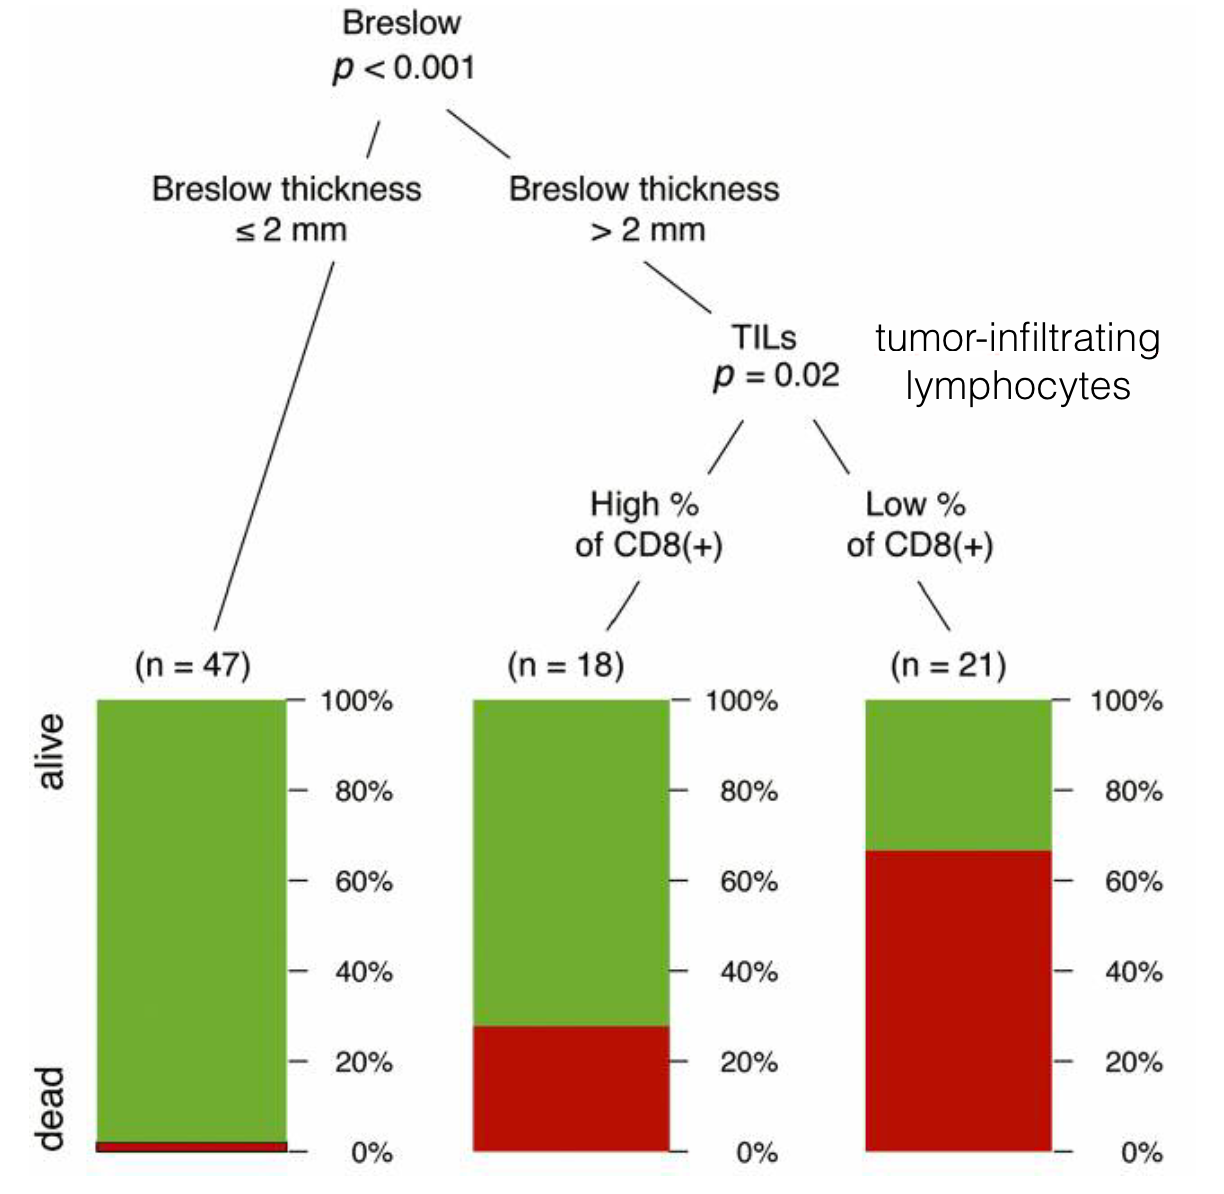
\includegraphics[width=0.5\linewidth]{figure/wbBILL8model} 

}

\caption{(fig:BILLCD8) Example tree model for melanoma risk}\label{fig:BILLCD8}
\end{figure}

\hypertarget{how-model-exploration-is-different-from-data-exploration}{%
\subsection{How model exploration is different from data
exploration?}\label{how-model-exploration-is-different-from-data-exploration}}

Exploration and visualization of models is not that known as exploration
and visualization of data.

In both data and model visualization we use a graphical representation
to deliver messages quicker in a form that is easier to digest. In fact,
we may use similar charts and similar way to express ideas. This is
because many people are already familiar with techniques for data
visualization and we may want to take advantage of this knowledge when
approaching model visualization.

Despite the similarites, we need to keep in mind a few key differences
between these two worlds.

First, with data exploration and visualization we want to understand
the, usually unknown, mechanism generating data. Models are created
based on the data, but in most cases we do not know how adequatly do
these models capture the unknown mechanism. So, we use model exploration
to check if the model is consistent with the data and, therefore, if it
may offer a description of the mechanism. However, in most cases we do
not check if data are ,,correct''. So, we are more skeptical about
models than about data.

Second, we usually treat data as a random sample coming from a
population or from a probability distribution. Hence, data inherit
randomness related to the sampling. On the other hand, models are just
functions. Most models are not stochastic (or at least some models are
not stochastic) and the randomness (if any) come from the fitting
procedure not from the sampling. {[}TOMASZ: NOT SURE WHAT DO WE WANT TO
SAY HERE?{]}

Finally, models may be inaccurate or biased. When we ask a question like
,,How does the model perform?'' we essentially ask, a t the same time,
,,is the model accurate? how much I can trust it?'`. With respect to
data, we often do not question their accuracy or ,,trustwothiness'', but
rather our understanding of the data. {[}TOMASZ: NOT SURE WHAT DO WE
WANT TO SAY HERE?{]}

Thus, in summary, we may use similar exploration and visualization
techniques for models and data. But the techniques are used to answer
different questions.

\hypertarget{model-agnostic-vs.model-specific-approach}{%
\subsection{Model-agnostic vs.~model-specific
approach}\label{model-agnostic-vs.model-specific-approach}}

Some classes of models attract higher interest or have been developed
for a longer period of time. Consequently, those classes of models are
equipped with very good tools for model exploration or visualisation.
For example:

\begin{itemize}
\tightlist
\item
  Linear models have got many tools for model diagnostics and
  evaluation. Model assumptions are formally defined (normality, linear
  structure, homogenous variance) and can be checked by using normality
  tests or plots (normal qq-plot), diagnostic plots, tests for model
  structure (RESET test), tools for identification of outliers, etc.
\item
  More complex models with an additive structure, like proportional
  hazards model, have also got many tools that can be used for checking
  model assumptions.
\item
  Random-forest model is equipped with out-of-bag method of evaluation
  of performance and several tools for measuring variable importance
  \citep{R-randomForest}. Methods have been developed to extract
  information from the model structure about possible interactions
  \citep{R-randomForestExplainer}. Similar tools are developed for other
  ensembles of trees, like xgboost models \citep{R-xgboostExplainer}.
\item
  Neural networks enjoy a large collection of dedicated explainers that
  use, for instance, the layer-wise relevance propagation technique
  \citep{BachLWRP}, or saliency maps technique \citep{SaliencyMaps}, or
  a mixed approach.
\end{itemize}

Of course, the list of model classes with dedicated collections of
model-explanation and/or diagnostics methods is much longer. This
variety of model-specific approaches does lead to issues, though. For
instance, one cannot easily compare explanations for two models with
different structures. Also, every time when a new architecture or a new
ensemble of models is proposed, one needs to look for new methods of
model exploration. Finally, for brand-new models no tools for model
explanation or diagnostics may be immedaitely available.

For these reasons, in our book we focus on model-agnostic techniques. In
particular, we prefer not to assume anything about the model structure,
as we may be dealing with a black-box model with an unclear structure.
In that case, the only operation that we may be able to perform is
evaluation of a model for a selected observation.

Hoever, while we do not assume anything about the structure of the
model, we will assume that the model operates on \(p\)-dimensional
vectors and, for a single vector, it returns a single value which is a
real number. This assumption holds for a broad range of models for data
such as tabular data, images, text data, videos, etc. It may not be
suitable for, e.g., models with memory in which the model output does
not depend only on the model input {[}TOMASZ: NOT SURE WHICH MODELS ARE
MEANT HERE{]}.

Note that the techniques considered in the book may not be sufficient to
fully understand models in case \(p\) is large.

\hypertarget{why-do-we-need-model-explainers}{%
\subsection{Why do we need model
explainers?}\label{why-do-we-need-model-explainers}}

Machine-learning models (MLMs) have a wide range of applications. Due to
the increasing computational power of computers and complexity of data
sources, MLMs are becoming more and more sophisticated. Models created
with the use of techniques such as boosting or bagging of neural
networks are parametrized by thousands of coefficients. They are
obscure; it is hard to trace the link between input variables and model
outcomes - in fact they are treated as black boxes. They are used
because of their elasticity and high performance, but their deficiency
in interpretability is one of their weakest sides.

In many applications we need to know, understand or prove how the input
variables are used in the model. We need to know the impact of
particular variables on the final model predictions. Thus we need tools
that extract useful information from thousands of model parameters.

Tools for model exploration and model understanding have many
applications. They may be useful during every phase of a model
lifecycle.

Below we summaries how such tools will be useful during the model
development, model deployment or model maintenance.

\begin{figure}

{\centering 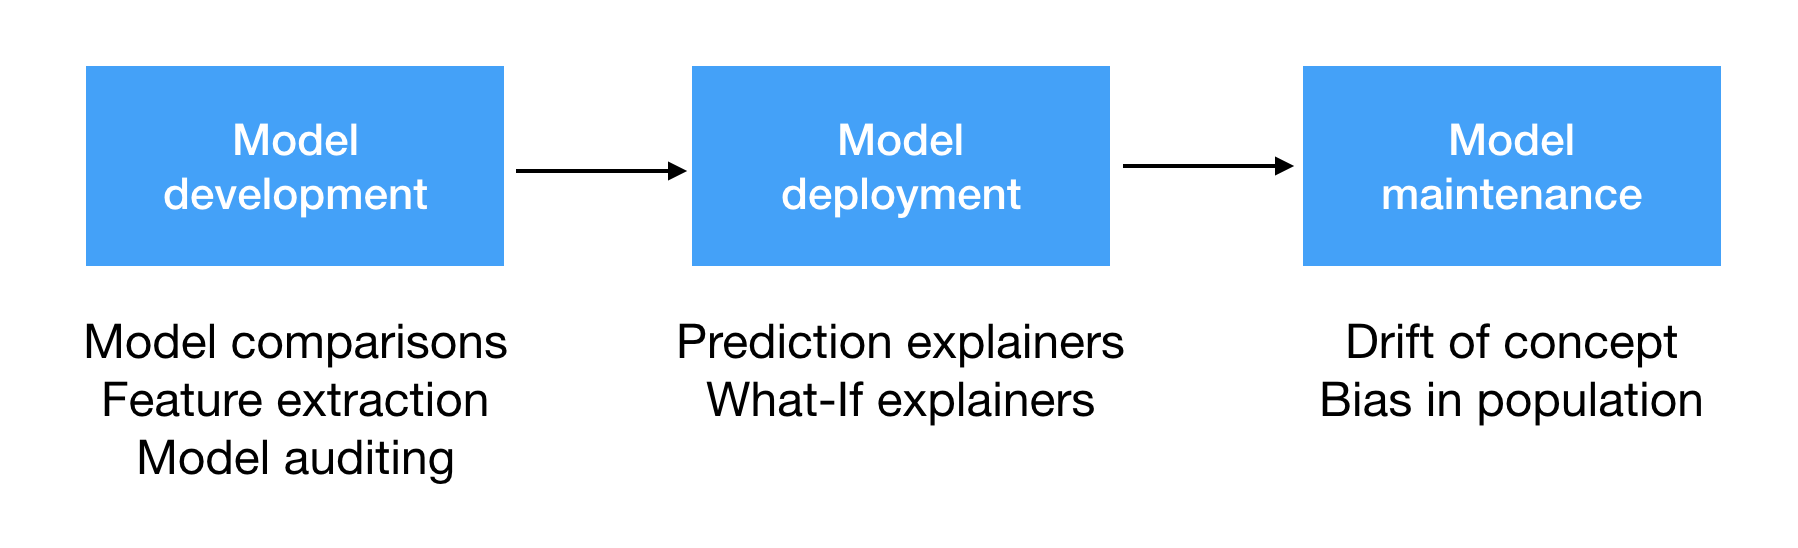
\includegraphics[width=0.9\linewidth]{figure/modelLifetime} 

}

\caption{(fig:modelLifetime) Example applications of explainers in different phases of model lifetime}\label{fig:modelLifetime}
\end{figure}

\textbf{Model development}

Model building or model development is a phase in which one is looking
for best available model.

In the Section \ref{partialDependence} we present tools for extraction
of relations between features and target variable. Such methods may be
used for feature engineering (assisted learning in which elastic black
box model is used to learn features for the white box model). Learning
from ML models may lead to model improvment.

In the Section \ref{modelComparisons} we present tools that helps to
compare models.

In the Section \ref{modelAuditing} we present tools that help to
validate model, audit model residuals, identify potential strange
behaviors.

If for some observations we observe lack of fit, then through tools
introduced in the Section \ref{variableAttributionMethods} we may verify
which variables do and which do not influence model decisions. This may
help to identify some problem in the model fit and in the end will help
to correct the model.

Since the AutoML methods are being more and more popular, model
explainers may actually help to understand how the model identified by
AutoML method is working.

If we identify cases on which model is not working properly, then model
explainers will help in model debugging. See an examples in the Section
TODO.

\textbf{Model deployment}

Model deployment is a phase in which one wants final use trust in model
decisions, understand these decisions and act accordingly. In some areas
complex models are not being adopted because people do not understand
nor trust them. Model explainers can change this and increase rate of
aquisition of new models

Since most people would not trust in recommendations, that they do not
understand, the key element here is to increase understanding related to
features that affect model decisions.

In the Section \ref{variableAttributionMethods} we introduce tools that
identify key features that drive model decisions.

In the Section \ref{ceterisParibus} we introduce tools for what-if
analysis of model decisions.

In some areas there may be leagal expectations or regulations that
requires that model predictions are explainable (see the right to
explanation). See \citep{2017arXiv171107076L} or
\citep{2017arXiv171006169T} for example methods that identify bias in
the data.

\textbf{Model maintenance}

Model maintenance is a phase in which one wants to make sure that model
is still valid and suited to the new data. Due to concept drift or
similar problems that may happen after some time, we need to monitor the
model performance.

In the section \ref{partialDependence} we present tools that may compare
how thw model response behaves on the new dataset. This helps to detect
flaws in model assumptions and biases in the data.

\hypertarget{model-lifecycle}{%
\subsection{Model lifecycle}\label{model-lifecycle}}

Figure \ref{fig:lifecycle} shows typical lifecycle of a predictive
model. Part of the lifecycle are activities that lead to the model
development. First, of course, we need to understand the domain of a
problem, then we need to select important features, prepare important
features, select the right model structure and viola! We have the model.

Once the model is created we still need to validate its performance. We
need to support its deployment and maintenance.

\begin{figure}

{\centering 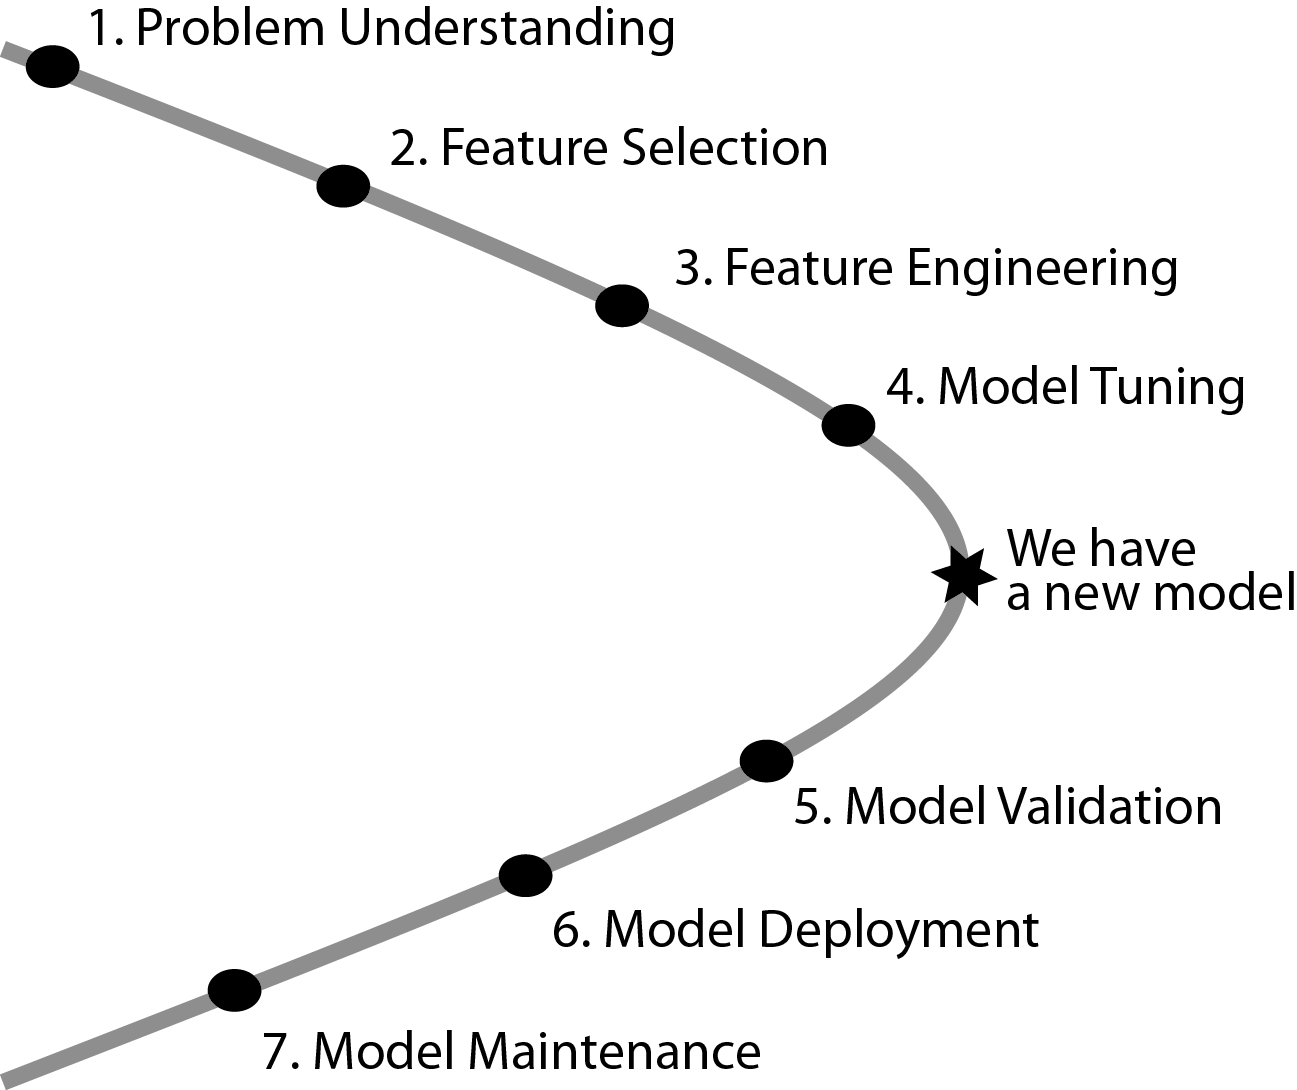
\includegraphics[width=0.5\linewidth]{figure/lifecycle} 

}

\caption{(fig:lifecycle) Model lifecycle}\label{fig:lifecycle2}
\end{figure}

As we will show, tools for model exploration, explanation and
visualization may be useful in every phase of model lifecycle.

\begin{itemize}
\tightlist
\item
  Tools presented in chapter \ref{variableImportance} helps to
  understand variable importance. They can be used in phase 2 - features
  selection.
\item
  Tools presented in chapter \ref{variableRelation} helps to understand
  variable effect. They can be used in phase 3 - features engineering.
\end{itemize}

Once the model is created, tools for model uderstanding have in general
two applications.

\begin{itemize}
\tightlist
\item
  We can use them to contrast model behavior with our domain knowledge.
  This way we can validate if model behavior is consistent with our
  expectations / some imposed requirements.
\item
  We can use them to extract some new knowledge about the domain. One
  possible application is to train a very elastic model to the dataset
  and then use model explainers to better understand relation between
  input variables and the target variable.
\end{itemize}

After model creation we may use model explainers to:

\begin{itemize}
\tightlist
\item
  Validate the model, some tools for that are presented in chapter
  \ldots{}.
\item
  Deploy the model. For deployed models we are interested in arguments
  agains particular decisions.
\item
  Maintain the model. Monitor concept drift for a model.
\end{itemize}

\hypertarget{code-snippets}{%
\subsection{Code snippets}\label{code-snippets}}

TODO: Here we should tell why we present examples for DALEX. And mention
that there are also other functions that can be used.

\hypertarget{glossary-notation}{%
\subsection{Glossary / Notation}\label{glossary-notation}}

Let \(f_{M}(x): \mathcal R^{d} \rightarrow \mathcal R\) denote a
predictive model, i.e.~function that takes \(d\) dimensional vector and
calculate numerical score. Dimenstions of the vector \(x\) refer to
different variables (aka features).

In sections in which we work with larger number of models we use
subscript \(M\) to index models. But to simplify notation, this
subscript is omitted if profiles for only one model are considered.

Symbol \(x \in \mathcal R^d\) refers to a point in the feature space. We
use subscript \(x_i\) to refer to a different data points and
superscript \(x^j\) to refer to specific dimensions. Additionally, let
\(x^{-j}\) denote all coordinates except \(j\)-th and let \(x|^j=z\)
denote a data point \(x^*\) with all coordinates equal to \(x\) except
coordinate \(j\) equal to value \(z\). I.e.
\(\forall_{i \neq {j}} x^i = x^{*,i}\) and \(x^j = z\). In other words
\(x|^j=z\) denote a \(x\) with \(j\)th coordinate changed to \(z\).

\begin{itemize}
\tightlist
\item
  \emph{Black-box model} is a model with structure that is hard to
  understand for humans. Usually it refers to the number of model
  parameters. As different humans may be better in understanding more or
  less complex models, there is no strict threshold that makes model a
  black-box. But in practice for most humans this threshold is closed to
  10 rather than 100.
\item
  \emph{White-box model}, opposite to Black-box model, is a model that
  is easy to understand to human. Maybe not for every human. Consider
  small linear models and small CAR trees as white box models.
\item
  \emph{Feature} or \emph{Variable}, part of the model input space.
  Without large loss of generality we can assume that one feature is a
  single dimension in the input space. There are exceptions (among them:
  polynomials, interactions between variables, nominal variables), but
  they do not change the intuition.
\item
  \emph{Continuous variable}, a variable that can be presented as a
  number and the ordering makes some sense (zip codes or phone numbers
  are not considered as continuous variables). It does not need to be
  continuous in a mathematical sense. Counting variables (number of
  floors, steps) counts here as well.
\item
  \emph{Nominal variable}, opposite to \emph{Continuous variables},
  finite set of values that will not the threated as a numeric
\item
  \emph{Model level explanations}, opposite to \emph{Instance level
  explanations}. Techniques that are designed to extract information
  related to a model behaviour for a selected dataset, usualy validation
  dataset. Other names \emph{Population level explanations} (when we
  thing about the validation dataset as a sample from some popualtion),
  \emph{global level explanations} (opposite to \emph{individual}).
\item
  \emph{Instance level explanations}, opposite to \emph{Model level
  explanations}. Techniques that are designed to extract information
  about model behaviour related to a specific observation or instance.
  Other names \emph{Individual level} (oposite to \emph{global}),
  \emph{Prediction level} (as this is related to a single model
  prediction).
\end{itemize}

\hypertarget{the-structure-of-the-book}{%
\subsection{The structure of the book}\label{the-structure-of-the-book}}

Our book is split in two parts. In the part \emph{Prediction level
explainers}, we present techniques for exploration and explanation of
model predictions for a single observation. On the other hand, in the
part \emph{Model level explainers}, we present techniques for
exploration and explanation of a model as a whole. In each part, every
method for model exploration is described in a separate section. The
method sections have got the same strucutre: * Subsection
\emph{Introduction} explains the goal of and the general idea behind the
method. * Subsection \emph{The Algorithm} shows mathematical or
computational details related to the method. This subsection can be
skipped if you are not interested in the details. * Subsection
\emph{Example} shows an exemplary application of the method with
discussion of results. * Subsection \emph{Pros and Cons} summarizes the
advantages and disadvantages of the method. It also provides some
guideance regarding when to use the method. * Subsection \emph{Code
snippets} shows the implementation of the method in R and Python. This
subsection can be skipped if you are not interested in the
implementation.

\textbf{In this book, we do show}

\begin{itemize}
\tightlist
\item
  how to determine features that affect model prediction for a single
  observation. In particular, we present the theory and examples of
  methods that can be used to explain prediction like break down plots,
  ceteris paribus profiles, local-model approximations, or Shapley
  values.
\item
  techniques to examine fully-trained machine-learning models as a
  whole. In particular, we review the theory and examples of methods
  that can be used to explain model performance globally, like
  partial-dependency plots, variable-importance plots, and others.
\item
  charts that can be used to present key information in a quick way.
\item
  tools and methods for model comparison.
\item
  code snippets for R and Python that explain how to use the described
  methods.
\end{itemize}

\textbf{In this book, we do not focus on}

\begin{itemize}
\tightlist
\item
  any specific model. The presented techniques are model agnostic and do
  not make any assumptions related to model structure.
\item
  data exploration. There are very good books on this topic, like R for
  Data Science \url{http://r4ds.had.co.nz/} or TODO
\item
  the process of model building. There are also very good books on this
  topic, see An Introduction to Statistical Learning by Gareth James,
  Daniela Witten, Trevor Hastie and Robert Tibshirani
  \url{http://www-bcf.usc.edu/~gareth/ISL/} or TODO
\item
  any particular tools for model building. These are discussed, for
  instance, in Applied Predictive Modeling By Max Kuhn and Kjell Johnson
  \url{http://appliedpredictivemodeling.com/}
\end{itemize}

It is worth noting that the same concepts have often been given
different names in statistics and in machine learning. Thus, before
embarking on the presentation of methods, in Section 1 we try to
,,translate'' the jargons used in these two worlds. In particular, we
introduce the notation and vocabulary that will be used throughout the
book. In this section, we also set expectations.

\hypertarget{thanksto}{%
\subsection{Acknowledgements}\label{thanksto}}

My work on interpretability has started during research trips within the
RENOIR project (691152 - H2020/2016-2019). So I would like to thank
prof. Janusz Holyst for the chance to take part in this project.

I would thank prof. Chris Drake for her hospitality. This book will
never been created without perfect conditions that I found at your house
in Woodland.

This book is prepared with the \textbf{bookdown} package
\citep{R-bookdown}, thanks to amazing work of Yihui Xie.

\hypertarget{model-lifecycle-1}{%
\subsection{Model lifecycle}\label{model-lifecycle-1}}

Figure \ref{fig:lifecycle} shows typical lifecycle of a predictive
model. Part of the lifecycle are activities that lead to the model
development. First, of course, we need to understand the domain of a
problem, then we need to select important features, prepare important
features, select the right model structure and viola! We have the model.

Once the model is created we still need to validate its performance. We
need to support its deployment and maintenance.

\begin{figure}

{\centering 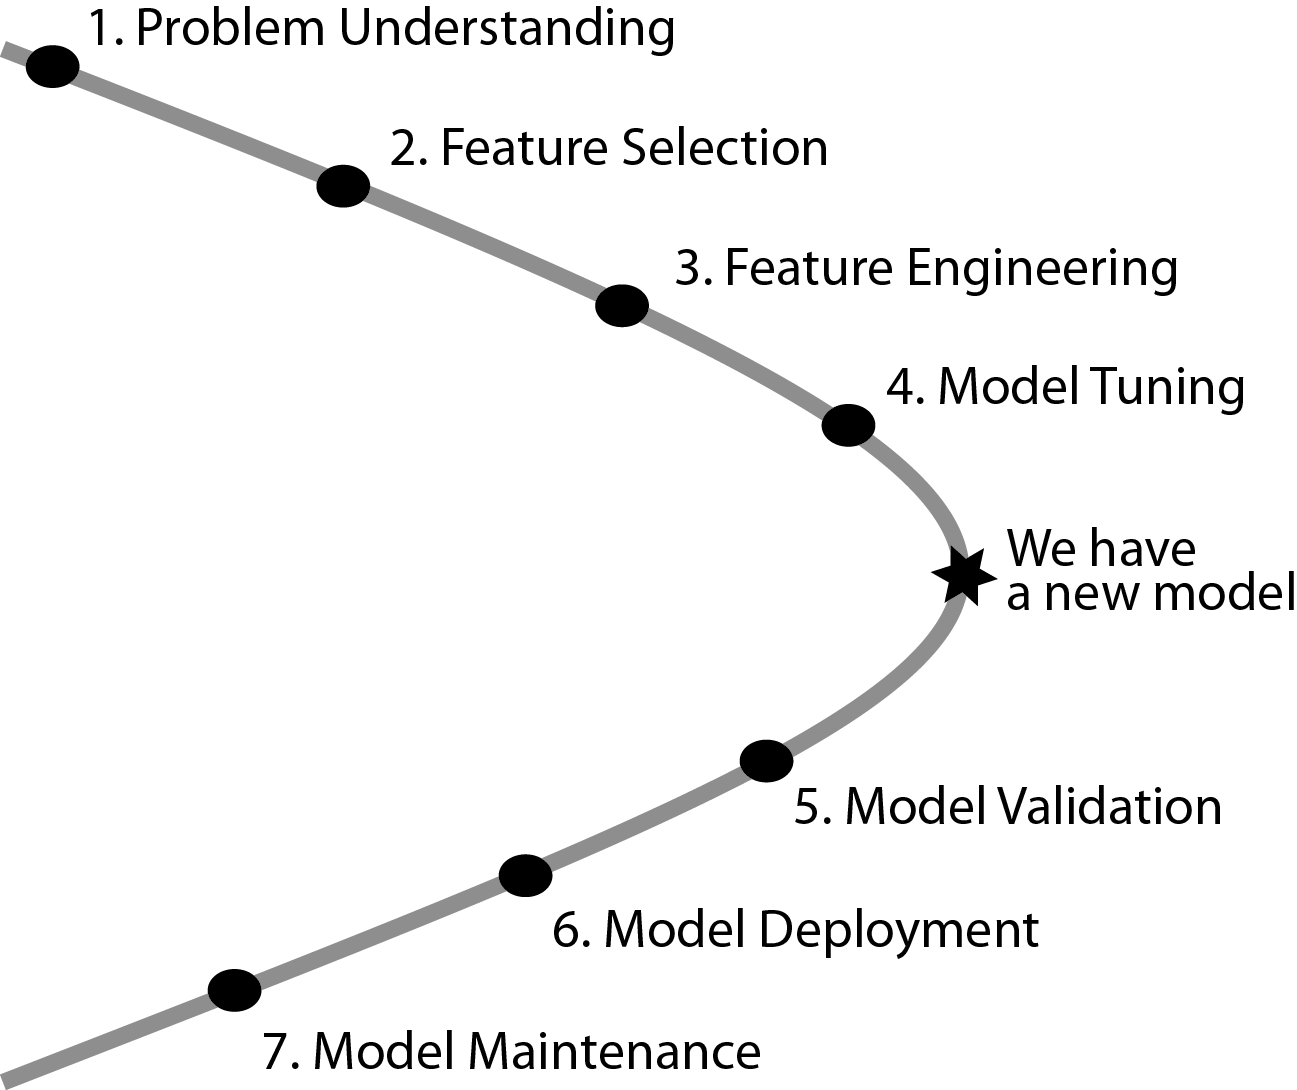
\includegraphics[width=0.5\linewidth]{figure/lifecycle} 

}

\caption{(fig:lifecycle) Model lifecycle}\label{fig:lifecycle}
\end{figure}

As we will show, tools for model exploration, explanation and
visualization may be useful in every phase of model lifecycle.

\begin{itemize}
\tightlist
\item
  Tools presented in chapter \ref{variableImportance} helps to
  understand variable importance. They can be used in phase 2 - features
  selection.
\item
  Tools presented in chapter \ref{variableRelation} helps to understand
  variable effect. They can be used in phase 3 - features engineering.
\end{itemize}

Once the model is created, tools for model uderstanding have in general
two applications.

\begin{itemize}
\tightlist
\item
  We can use them to contrast model behavior with our domain knowledge.
  This way we can validate if model behavior is consistent with our
  expectations / some imposed requirements.
\item
  We can use them to extract some new knowledge about the domain. One
  possible application is to train a very elastic model to the dataset
  and then use model explainers to better understand relation between
  input variables and the target variable.
\end{itemize}

After model creation we may use model explainers to:

\begin{itemize}
\tightlist
\item
  Validate the model, some tools for that are presented in chapter
  \ldots{}.
\item
  Deploy the model. For deployed models we are interested in arguments
  agains particular decisions.
\item
  Maintain the model. Monitor concept drift for a model.
\end{itemize}

\hypertarget{prediction-level-explanations}{%
\section*{Prediction level
explanations}\label{prediction-level-explanations}}
\addcontentsline{toc}{section}{Prediction level explanations}

\begin{figure}

{\centering 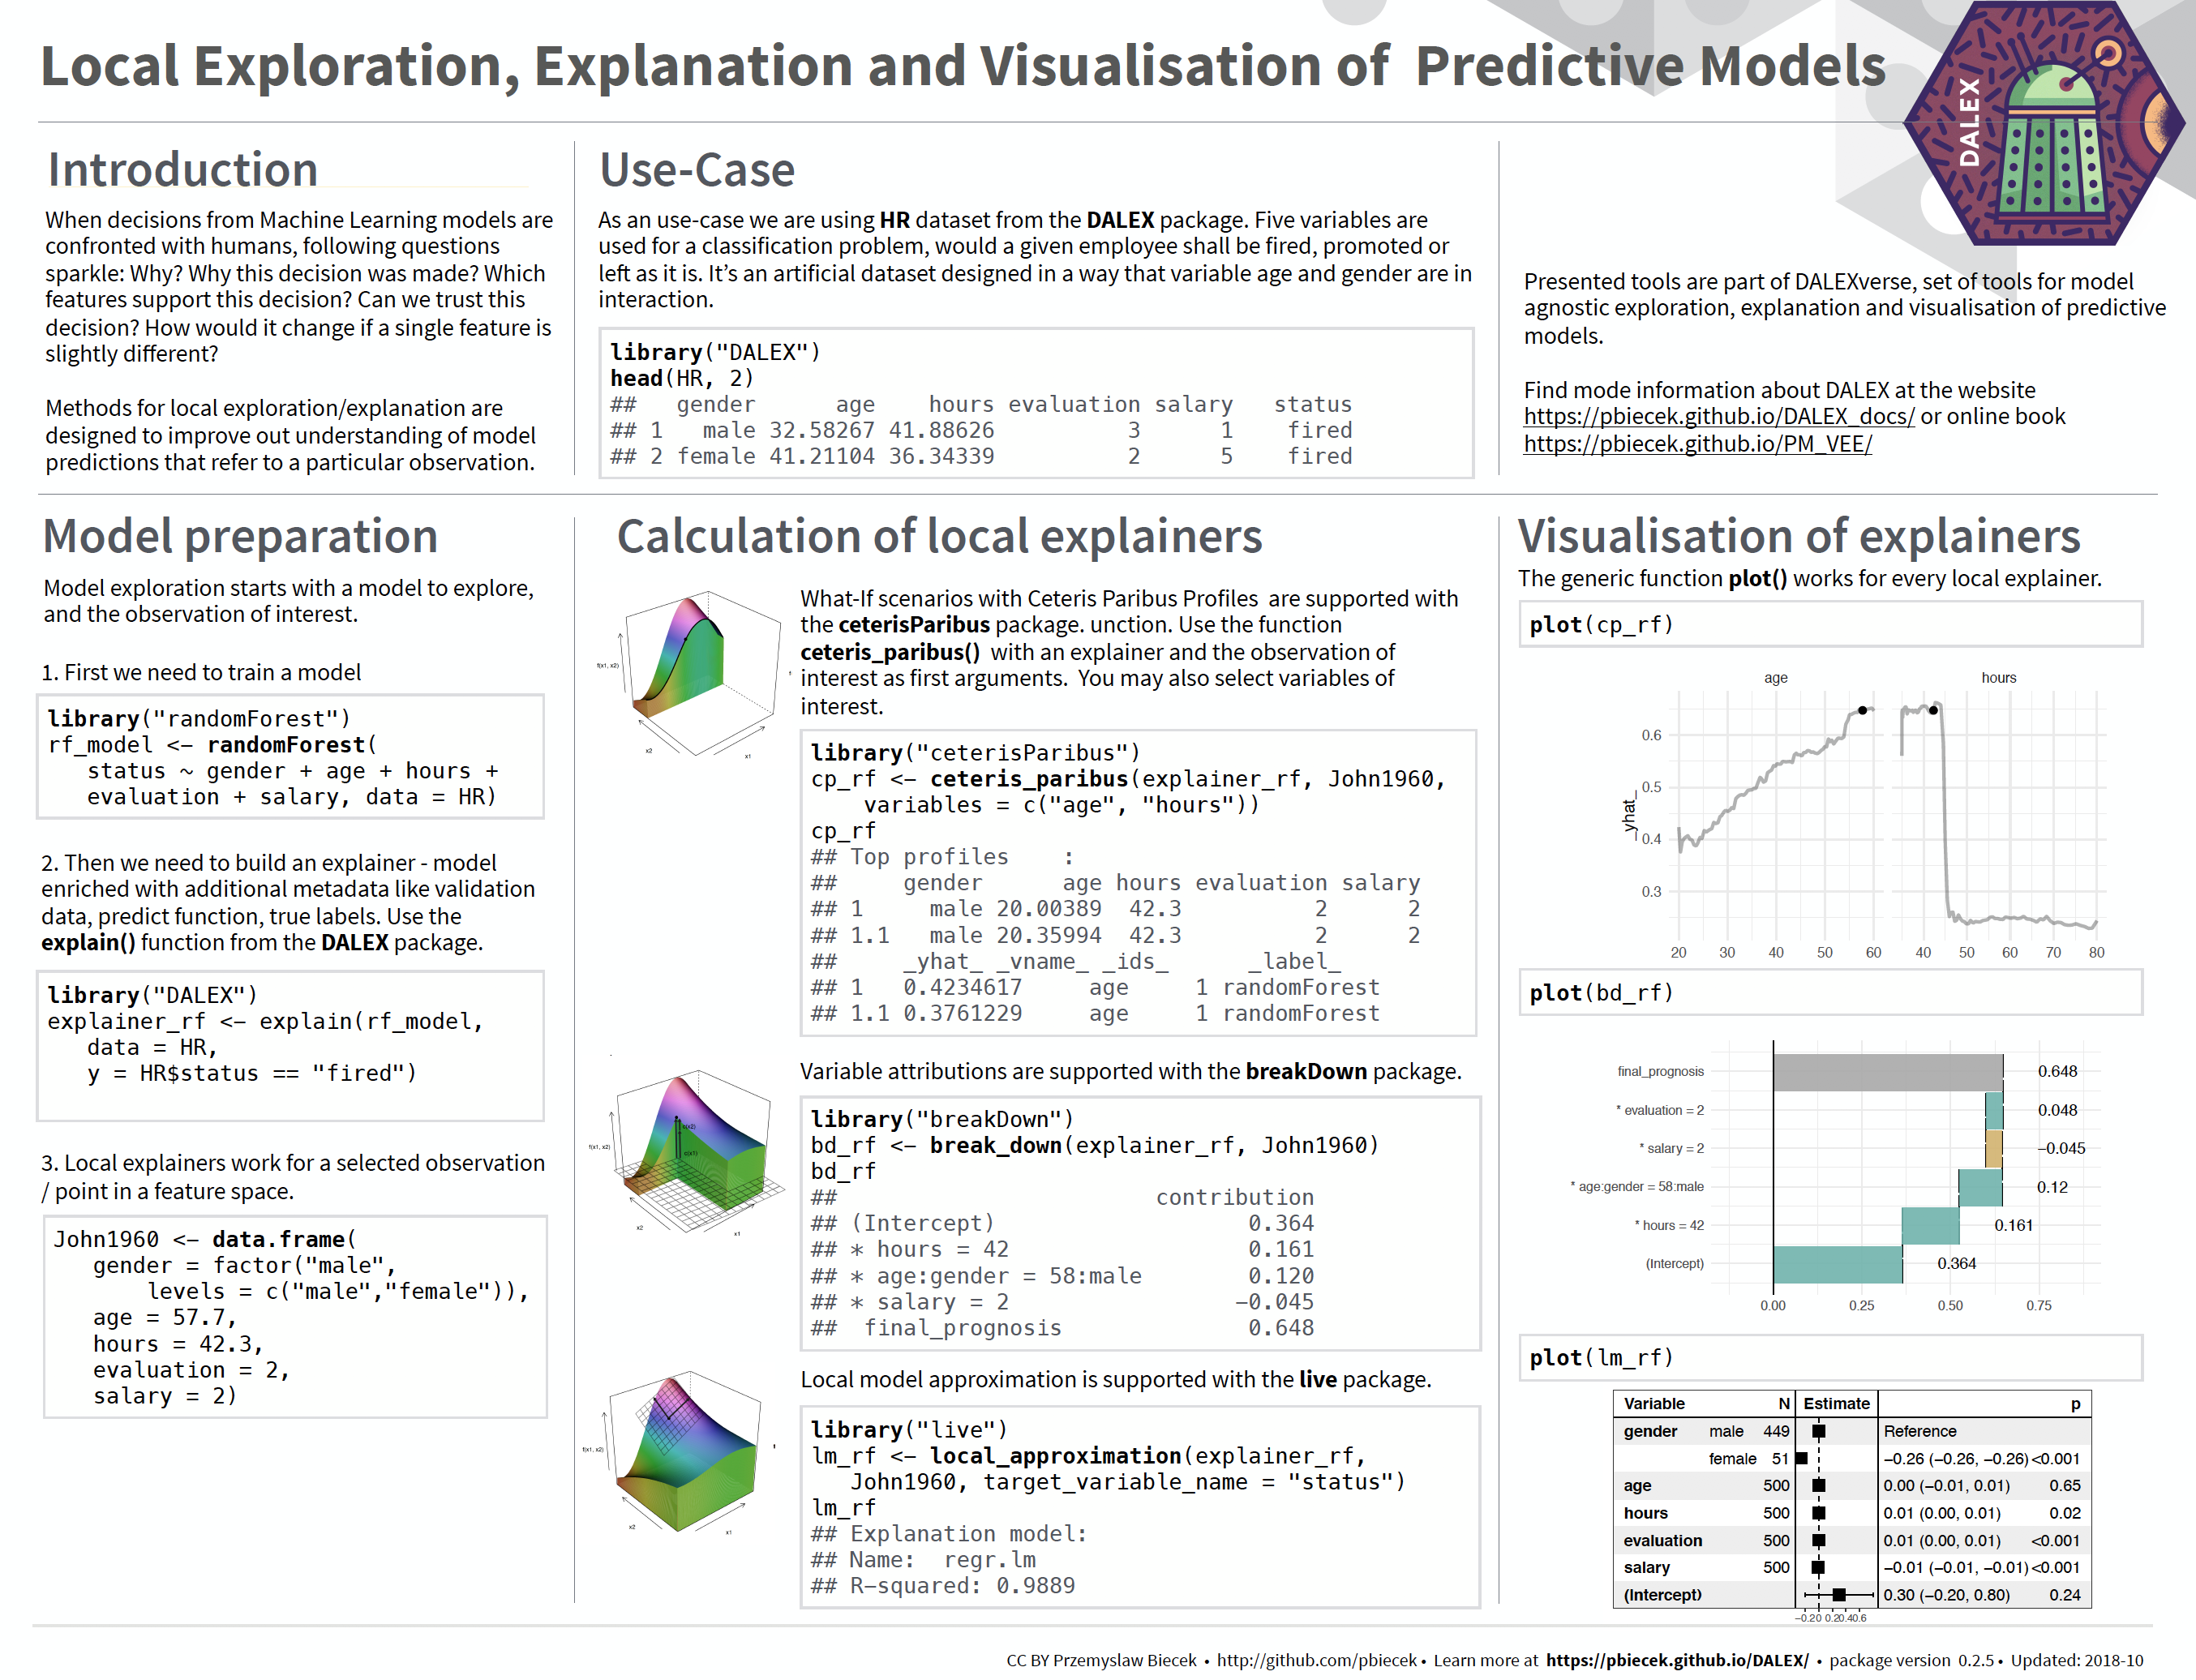
\includegraphics[width=0.99\linewidth]{figure/DALEX_local} 

}

\caption{(fig:localDALEXsummary) Summary of three approaches to local model exploration and explanation.}\label{fig:localDALEXsummary}
\end{figure}

\hypertarget{PredictionExplainers}{%
\section{Introduction}\label{PredictionExplainers}}

Prediction level explainers help to understand how the model works for a
single prediction. This is the main difference from the model level
explainers that were focused on the model as a whole and on model
population for whole population. Prediction level explainers work in the
context of single observations.

Think about following use-cases

\begin{itemize}
\tightlist
\item
  One wants to attribute effects of variables to a model predictions.
  Think about model for heart accident Having a final score for a
  particular patient one wants to understand how much of this score can
  be attributed to smoking or age or gender.
\item
  One wants to understand how the model response would change if some
  inputs are changed. Again, think about model for heart accident How
  the model response would change if a patient cuts the number of
  cigarettes per day by half. Or if he introduces a low-carbon diet.
\item
  Model is not working correctly for a particular point and one wants to
  understand why predictions for this point are wrong. Think about
  patient that had heart accident but his risk score is very low. One
  wants to understand which factors may be overlooked.
\end{itemize}

\hypertarget{approaches-to-prediction-explanations}{%
\subsection{Approaches to prediction
explanations}\label{approaches-to-prediction-explanations}}

There are many different tools that may be used to explore model around
a single point \(x^*\). Model is a function that takes \(p\) dimensional
vector as an input. Thus to plot this function we would need \(p+1\)
dimensions.

An toy example with \(p=2\) is presented in Figure
\ref{fig:cutsSurfaceReady}. We will use it as an illustration of key
ideas.

\begin{figure}

{\centering 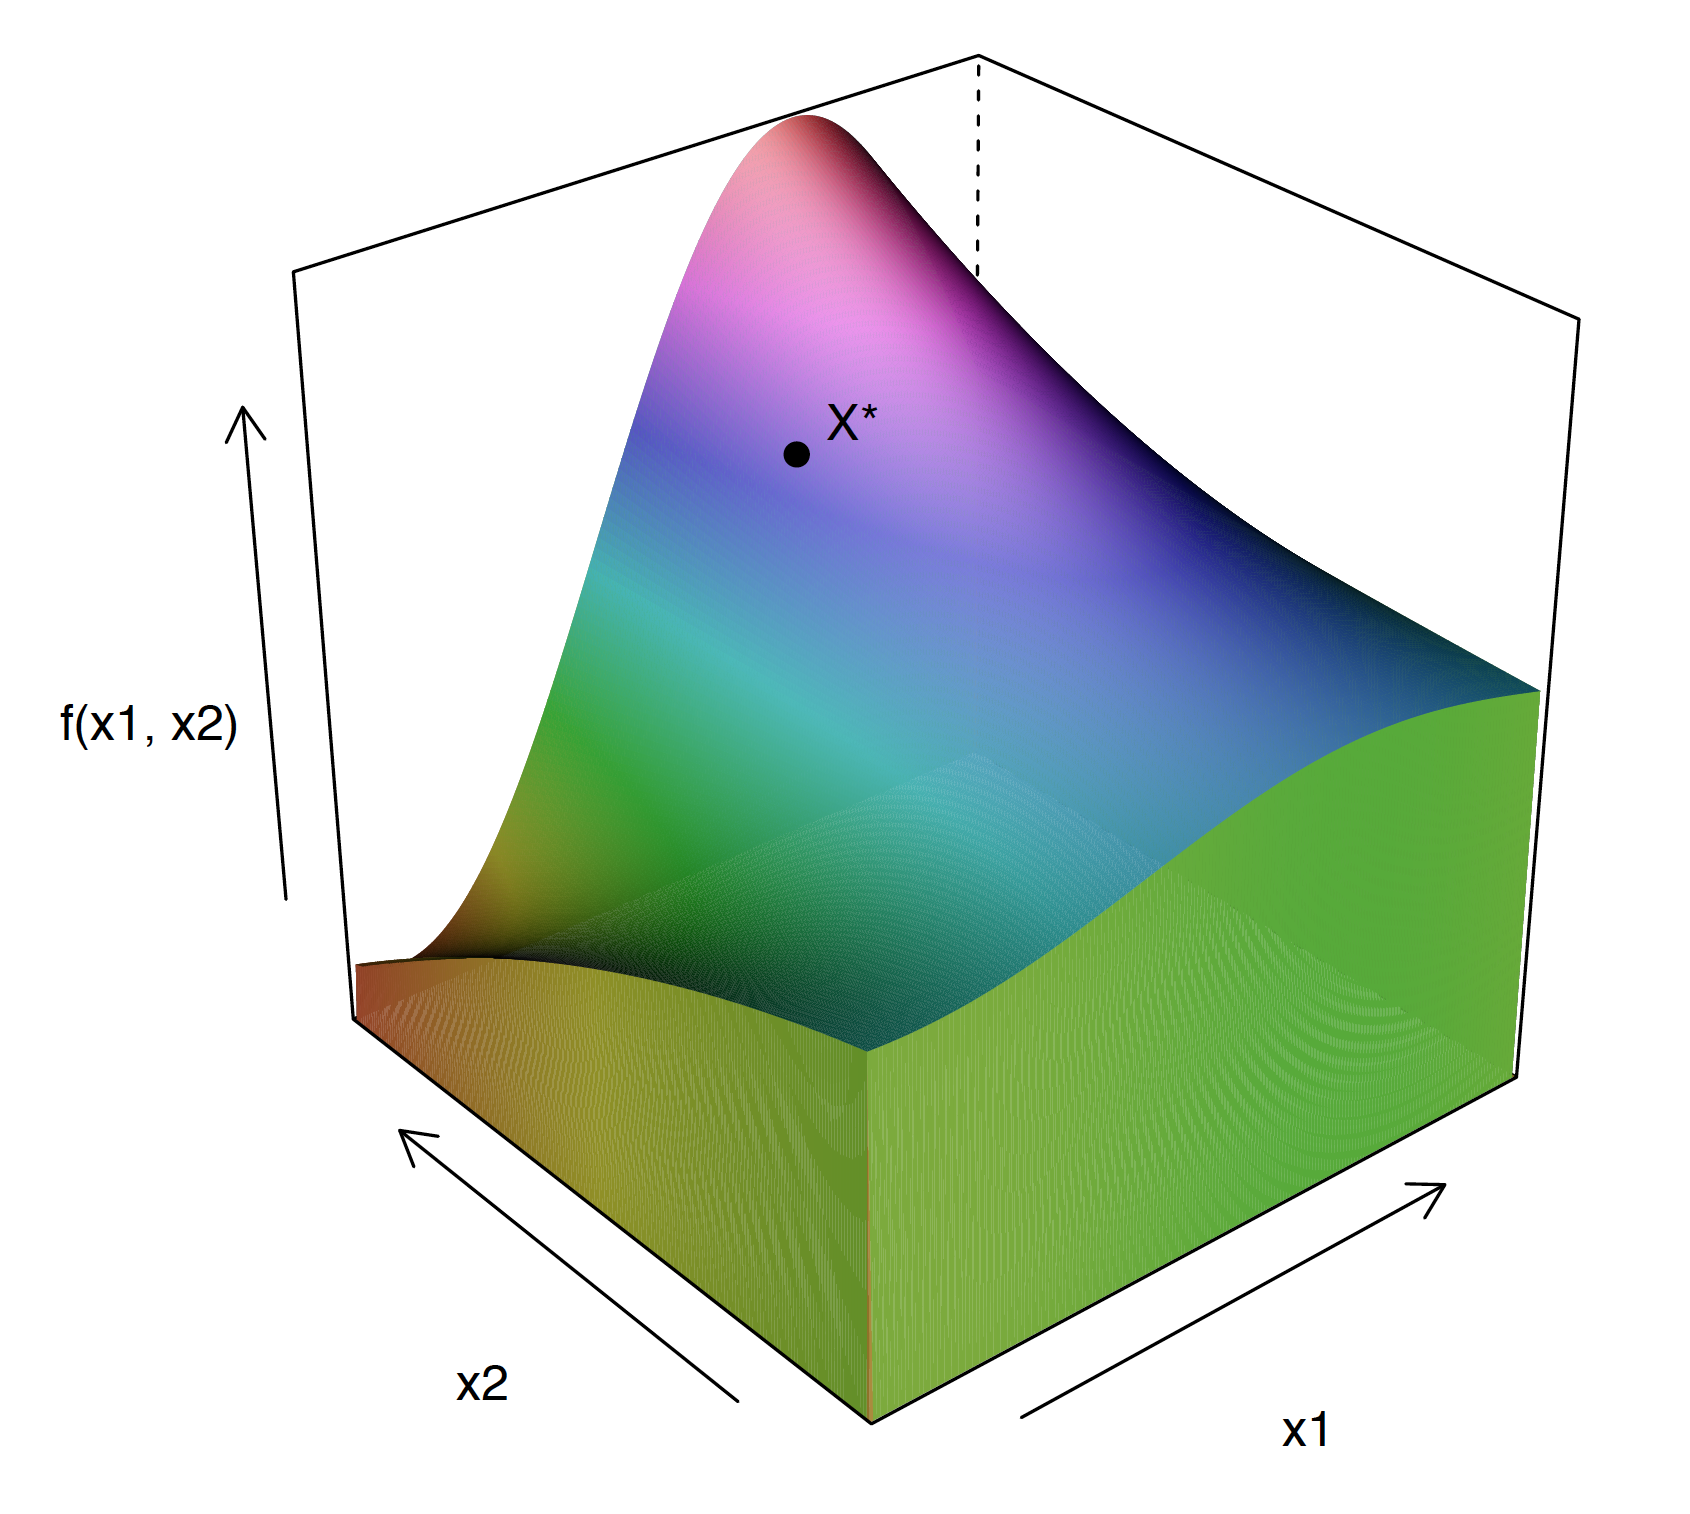
\includegraphics[width=0.6\linewidth]{figure/cuts_surface_ready_punkt} 

}

\caption{(fig:cutsSurfaceReady) Model response surface. Here the model is a function of two variables.  We are interested in understanding the response of a model in a single point x*}\label{fig:cutsSurfaceReady}
\end{figure}

In following sections we will describe the most popular approaches to
exploration of such function. They can be divided into three classes.

\begin{itemize}
\tightlist
\item
  One approach to exploration of model response is to investigate how
  the model response would change if single variable in the model input
  would change. This way we may observe profiles seen as a function of a
  single variable. Such profiles are usually called Ceteris Paribus
  Profiles. We will present them in detail in the Section
  \ref{ceterisParibus}. This is useful for What-If scenarios. See an
  example in Figure \ref{fig:cutsTechnikiReady} panel A.
\item
  Other approach is to analyze model curvature around point of interest.
  Again we treat the model as a function and we are interested in the
  local behavior of this function around the point of interest. We
  approximate the black-box model with a simpler white-box model around
  point \(x^*\). See an example in Figure \ref{fig:cutsTechnikiReady}
  panel B. In the Section \ref{LIME} we present the LIME method that
  exploits the concept of local model.
\item
  Yet another approach is to analyze how the model response in point
  \(x^*\) is different from the average model response. And how the
  difference can be distributed between model behavior along different
  dimensions. See an example in Figure \ref{fig:cutsTechnikiReady} panel
  C. In the Section \ref{variableAttributionMethods} we present two
  methods for variable contributions, sequential conditioning and
  average conditioning (called also Shapley values).
\end{itemize}

\begin{figure}

{\centering 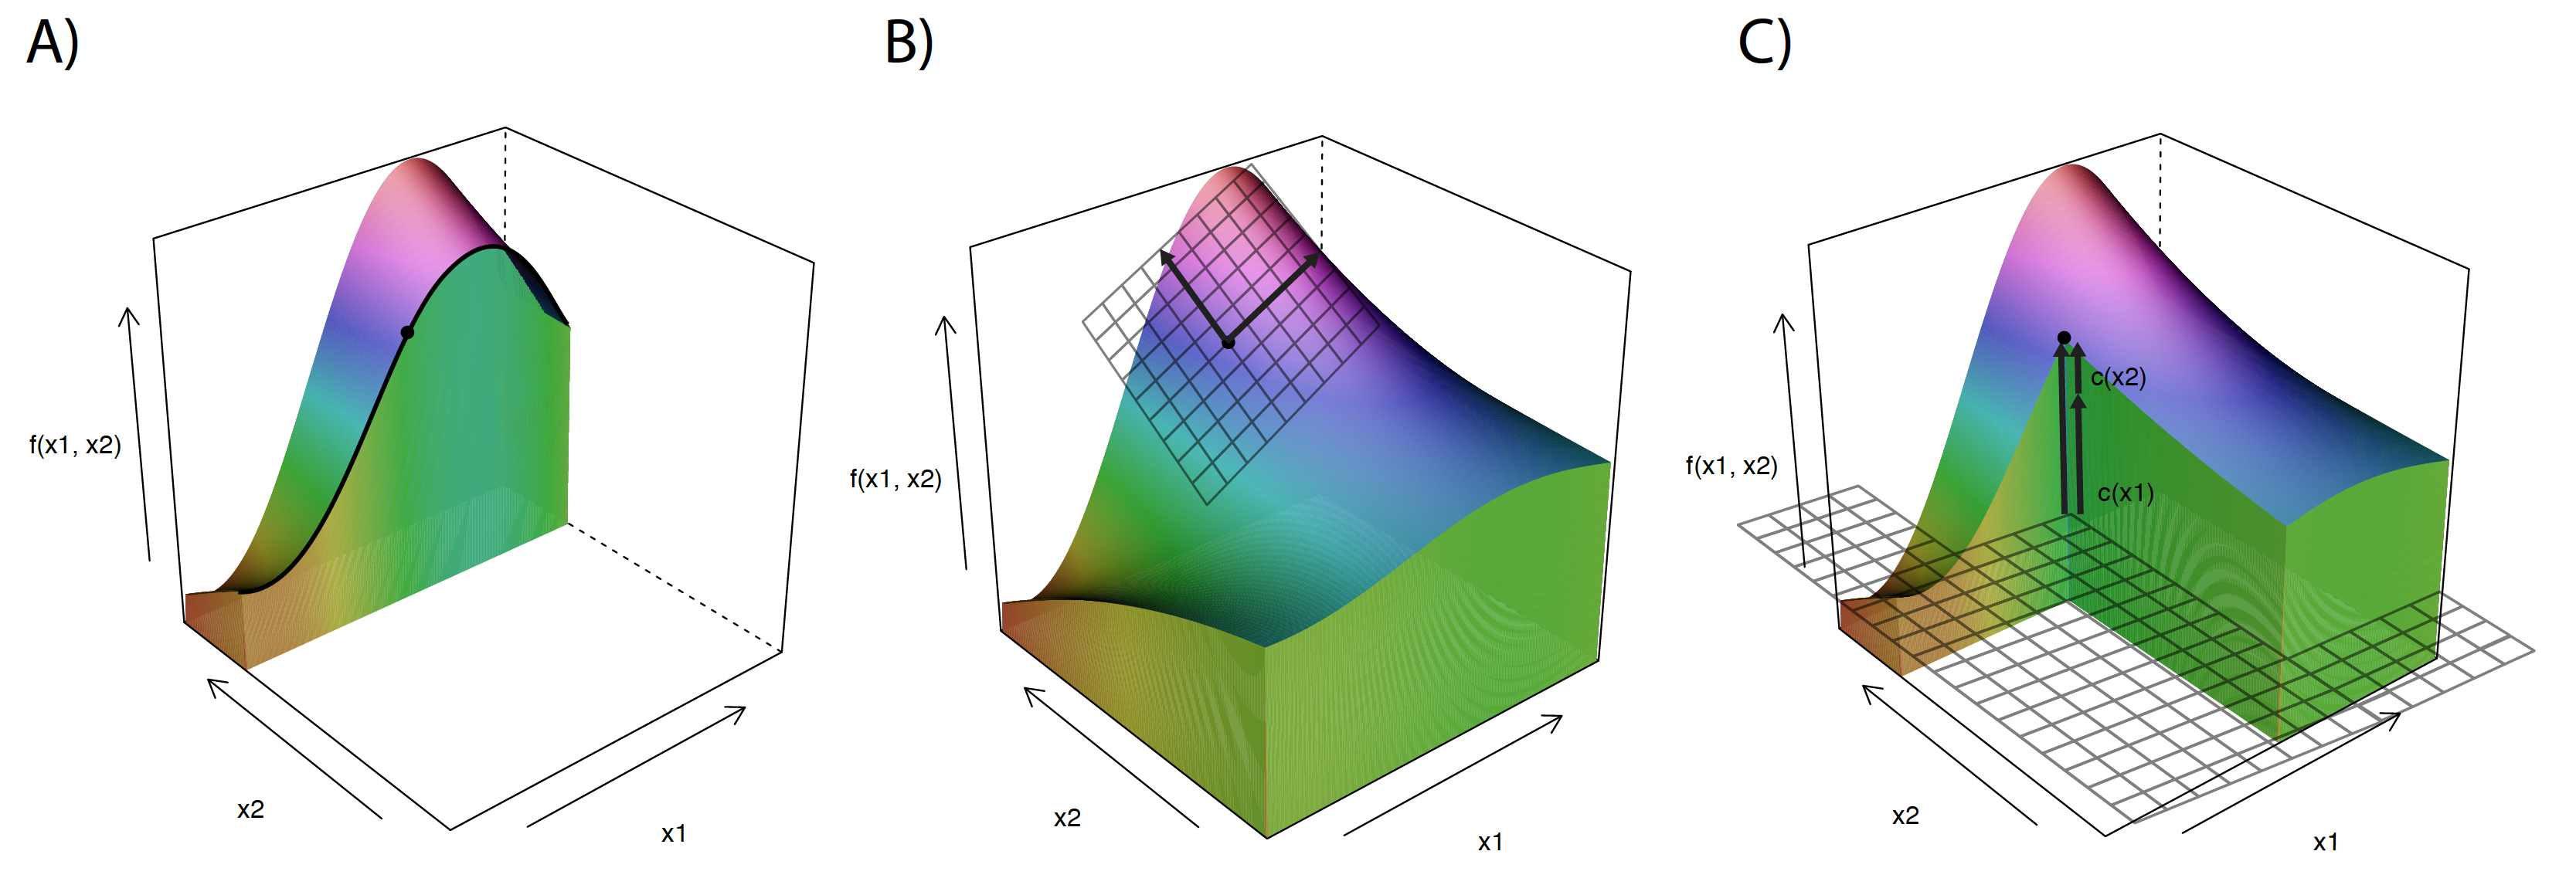
\includegraphics[width=0.99\linewidth]{figure/cuts_techniki_ready} 

}

\caption{(fig:cutsTechnikiReady) Intuitions behind different approached to prediction level explainers. Panel A presents an idea behind What-If analysis with Ceteris Paribus profiles. Keeping all other variables unchanged we trace model response along changes in a single variable. Panel B presents an idea behind local models like LIME. A simpler white-box model is fitted around the point of interest. It describes the local behaviour of the complex model. Panel C presents an idea behind variable attributions. Additive effects of each variable show how the model response differs from population average.}\label{fig:cutsTechnikiReady}
\end{figure}

\hypertarget{three-single-laws}{%
\subsection{A bit of philosophy: Three Laws for Prediction Level
Explanations}\label{three-single-laws}}

76 years ago Isaac Asimov devised
\href{https://en.wikipedia.org/wiki/Three_Laws_of_Robotics}{Three Laws
of Robotics}: 1) a robot may not injure a human being, 2) a robot must
obey the orders given it by human beings and 3) A robot must protect its
own existence. These laws impact discussion around
\href{https://en.wikipedia.org/wiki/Ethics_of_artificial_intelligence}{Ethics
of AI}. Today's robots, like cleaning robots, robotic pets or autonomous
cars are far from being conscious enough to be under Asimov's ethics.

Today we are surrounded by complex predictive algorithms used for
decision making. Machine learning models are used in health care,
politics, education, judiciary and many other areas. Black box
predictive models have far larger influence on our lives than physical
robots. Yet, applications of such models are left unregulated despite
many examples of their potential harmfulness. See \emph{Weapons of Math
Destruction} by Cathy O'Neil \citep{ONeil} for an excellent overview of
selected problems.

It's clear that we need to control algorithms that may affect us. Such
control is in our civic rights. Here we propose three requirements that
any predictive model should fulfill.

\begin{itemize}
\tightlist
\item
  \textbf{Prediction's justifications}. For every prediction of a model
  one should be able to understand which variables affect the prediction
  and how strongly. Variable attribution to final prediction.
\item
  \textbf{Prediction's speculations}. For every prediction of a model
  one should be able to understand how the model prediction would change
  if input variables were changed. Hypothesizing about what-if
  scenarios.
\item
  \textbf{Prediction's validations} For every prediction of a model one
  should be able to verify how strong are evidences that confirm this
  particular prediction.
\end{itemize}

There are two ways to comply with these requirements. One is to use only
models that fulfill these conditions by design. White-box models like
linear regression or decision trees. In many cases the price for
transparency is lower performance. The other way is to use approximated
explainers -- techniques that find only approximated answers, but work
for any black box model. Here we present such techniques.

\hypertarget{variableAttributionMethods}{%
\section{Variable attribution for linear
models}\label{variableAttributionMethods}}

In this section we introduce the concept and the intuition behind
additive decompositions of model predictions. The main goal for these
tools is to help to understand how model output may be decomposed into
parts, that can be attributed to input features.

Presented explainers are linked with the first law introduced in Section
\ref{three-single-laws}, i.e.~law for prediction's justifications. Note
that there is a collection of tools for variable attribution. In this
section we are focused on the general idea and examples for linear
models. Model agnostic approaches will be presented in sections
\ref{breakDown} and \ref{shapley}.

Think of following use cases:

\begin{itemize}
\tightlist
\item
  Think about a model for heart attack. A patient wants to know which
  factors have highest impact on the final heart risk score.
\item
  Think about a model for apartment prices. An investor wants to know
  how much of the final price may be attributed to the location of an
  apartment.
\item
  Think about a model for credit scoring. A customer wants to know if
  factors like gender, age or number of kids influence model decisions.
\end{itemize}

In every usecase one needs to attribute part of the model response to a
single variable. This can be done directly for linear models, so in the
section \ref{VAlinMod} we show how to do this for linar models and may
be easily extended to additive models and generalized linear models. For
other models it is not trivial how to do so, some approaches are be
presented in next sections.

\hypertarget{intuition}{%
\subsection{Intuition}\label{intuition}}

Fiited linear model with coefficients
\(\beta = (\beta_0, \beta_1, .., \beta_p)\) has following form.

\[
f(x) = \beta_0 + x_1 \beta_1 + \ldots + x_p \beta_p.
\] In other words, model response is the sum of weighted elements of
\(x = (x_1, x_2, \ldots, x_p)\).

From a global perspective of a model, we are usually interested in
questions like, how good is the model (questions about \(R^2\)), which
variables are significant (tests for significance of \(\beta_i \neq 0\))
or how accurate are model predictions (confidence intervals for
predictions).

But in this chapter we are focued on a local perspective, i.e.~for a
single observation \(x^*\) how to measure the contribution of a variable
\(x_i\) on model prediction \(f(x^*)\).

The contribution of a variable \(x_i\) shall be related to
\(x^*_i\beta_i\) as variable \(x_i\) occur only in this term. As we will
see below, it is easier to interpret variable contribution if the
\(x_i\) is centered.

This lead for a intuitive formula for variable attribution for model
\(f\), variable \(x_i\) in the point \(x^*\) \[
v(f, x^*, i) = \beta_i (x_i^* - \hat x_i).
\]

\hypertarget{method}{%
\subsection{Method}\label{method}}

We want to calculate \(v(f, x^*, i)\), which is the contribution of
variable \(x_i\) on prediction of model \(f()\) in point \(x^*\).

Geneal approach for calculation of variable attributions would be to
measure how much the expected model response would change after
conditioning on \(x_i = x_i^*\).

\[
v(f, x^*, i) = E[f(x) | x_i = x_i^*] - E[f(x)]
\]

For linear models, if coordinates of \(x\) are independent, this is
equivalent of

\[
v(f, x^*, i) = f(x^*) - E[f(x)|x_{-i} = x^*_{-i}] = \beta_i x^*_i  - E \beta_i X_i.
\] Expected value can be estimated as averages, and this leads to\\
\[
v(f, x^*, i) = \beta_i x^*_i - \beta_i \bar x_i = \beta_i (x^*_i - \bar x_i)
\]

The logic behind the attribution is the following. Contribution of
variable \(x_i\) is the difference between model response for value
\(x_i^*\) minus the average model response.

Note that the linear model ma be rewritten in a following way

\[
f(x) = baseline + (x_1 - \bar x_1) \beta_1 + ... + (x_p - \bar x_p) \beta_p
\]

where \[
baseline = \mu + \bar x_1 \beta_1 + ... + \bar x_p \beta_p.
\]

Here \(baseline\) is an average model response and variable
contributions show how prediction for particular \(x^*\) is different
from the average response.

** NOTE for careful readers **

There is a gap between expected value of \(X_i\) and average calculated
on some dataset \(\bar x_i\). The latter depends on the data used for
calculation of averages. For the sake of simplicity we do not emphasize
these differences. To live with this just assume that we have access to
a very large validation data that allows us to calculate \(\bar x_i\)
very accurately.

Also we assumed that coordinated of \(x\) are independent, which may not
be the case. We will return to this problem later, during the discussion
related to interactions.

\hypertarget{example-wine-quality}{%
\subsection{Example: Wine quality}\label{example-wine-quality}}

It may be a surprise, that the attribution for variable \(x_i\) is not
the \(\beta_i x_i\). To understand this, consider following example.

\begin{figure}

{\centering 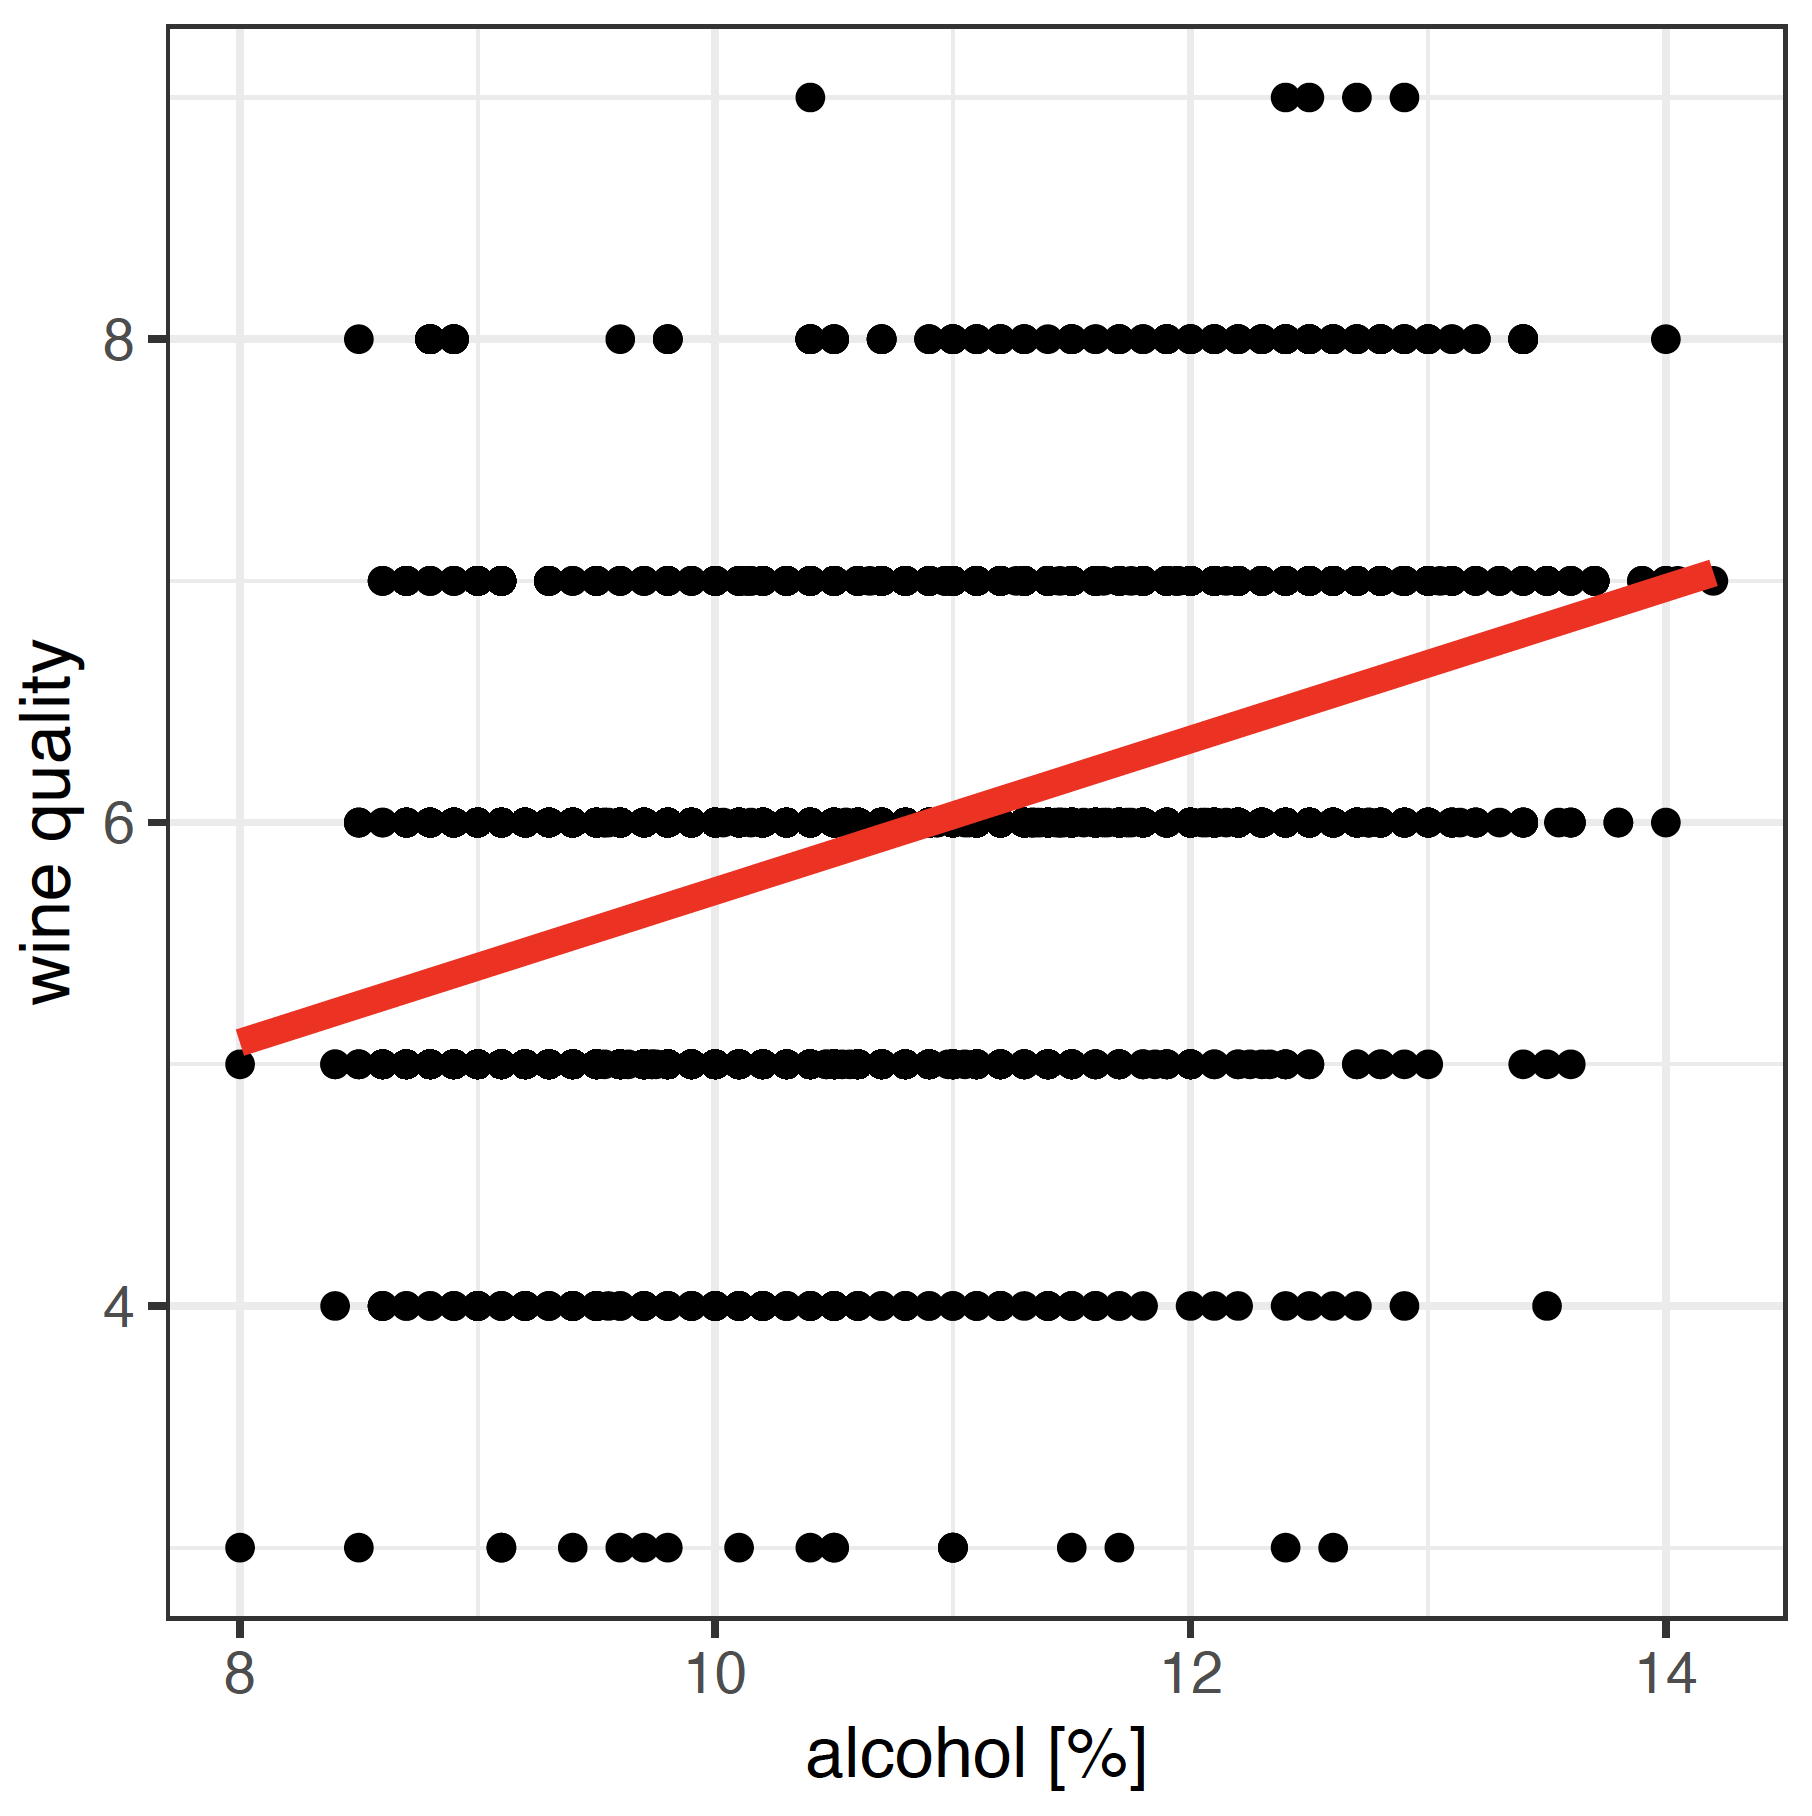
\includegraphics[width=0.5\linewidth]{figure/attribution_1} 

}

\caption{(fig:attribution1)Relation between wine quality and concentration of alcohol assessed with linear model}\label{fig:attribution1}
\end{figure}

Figure \ref{fig:attribution1} shows the relation between alcohol and
wine quality, based on the wine dataset \citep{wine2009}. The
corresponding linear model is

\[
quality(alcohol) = 2.5820 + 0.3135 * alcohol
\]

The weakest wine in this dataset has 8\% of alcohol, average alcohol
concentration is 10.51, so the contribution of alcohol to the model
prediction is \(0.3135 *(8-10.51) = -0.786885\). It means that low value
of alcohol for this wine (8\%) lower the prediction of quality by
\(-0.786885\).

Note, that it would be confusing to use \(x_i\beta_i\) as alcohol
contribution on quality would be \(0.3135*8 = 2.508\). This would not
reflect the intuition that for positive relation, the smaller is the
alcohol concentration the lower should be the quality of wine.

\hypertarget{pros-and-cons}{%
\subsection{Pros and Cons}\label{pros-and-cons}}

Here we summarise pros and cons of this approach.

\textbf{Pros}

\begin{itemize}
\tightlist
\item
  Presented variable attribution for linear model is not an
  approximation, it is directly linked with the structure of a model.
\item
  It is easier to understand attributions that are not linked with scale
  nor location of \(x_i\) as the standard \(\beta_i\) are.
\end{itemize}

\textbf{Cons}

\begin{itemize}
\tightlist
\item
  It works only for linear models.
\item
  This do not reduce model complexity. Just present model coefficients
  in a different way.
\end{itemize}

\hypertarget{code-snippets-1}{%
\subsection{Code snippets}\label{code-snippets-1}}

Variable attributions for linear models may be directly extracted from
the \texttt{predict()} function for linear models.

In this section we will present an example for logistic regression based
on the \texttt{HR} dataset. See the Section \ref{HRdataset} for more
details.

First we build a logistic regression model for binary variable
\texttt{status\ ==\ "fired"}. Here are fitted model coefficients.

\begin{Shaded}
\begin{Highlighting}[]
\KeywordTok{library}\NormalTok{(}\StringTok{"DALEX"}\NormalTok{)}
\NormalTok{model_fired <-}\StringTok{ }\KeywordTok{glm}\NormalTok{(status }\OperatorTok{==}\StringTok{ "fired"} \OperatorTok{~}\StringTok{ }\NormalTok{., }\DataTypeTok{data =}\NormalTok{ HR, }\DataTypeTok{family =} \StringTok{"binomial"}\NormalTok{)}
\KeywordTok{coef}\NormalTok{(model_fired)}
\end{Highlighting}
\end{Shaded}

\begin{verbatim}
##  (Intercept)   gendermale          age        hours   evaluation 
##  5.737945729 -0.066803609 -0.001503314 -0.102021120 -0.425793369 
##       salary 
## -0.015740080
\end{verbatim}

We want to calculate variable attributions for a particular point. Here
we define this point.

\begin{Shaded}
\begin{Highlighting}[]
\NormalTok{new_observation <-}\StringTok{ }\KeywordTok{data.frame}\NormalTok{(}\DataTypeTok{gender =} \KeywordTok{factor}\NormalTok{(}\StringTok{"male"}\NormalTok{, }\DataTypeTok{levels =} \KeywordTok{c}\NormalTok{(}\StringTok{"male"}\NormalTok{, }\StringTok{"female"}\NormalTok{)),}
                      \DataTypeTok{age =} \FloatTok{57.7}\NormalTok{,}
                      \DataTypeTok{hours =} \FloatTok{42.3}\NormalTok{,}
                      \DataTypeTok{evaluation =} \DecValTok{2}\NormalTok{,}
                      \DataTypeTok{salary =} \DecValTok{2}\NormalTok{)}
\end{Highlighting}
\end{Shaded}

For linear and generalized linear models we may specify argument
\texttt{type\ =\ "terms"} that extracts variable contributions.

\begin{Shaded}
\begin{Highlighting}[]
\KeywordTok{predict}\NormalTok{(model_fired, new_observation, }\DataTypeTok{type =} \StringTok{"terms"}\NormalTok{)}
\end{Highlighting}
\end{Shaded}

\begin{verbatim}
##        gender         age     hours evaluation      salary
## 1 -0.03361889 -0.02660691 0.7555555  0.5547197 0.007287334
## attr(,"constant")
## [1] -0.8714962
\end{verbatim}

Below we show how to do this with the \texttt{DALEX} package.
Additionaly we may easily plot contributions.

\begin{Shaded}
\begin{Highlighting}[]
\KeywordTok{library}\NormalTok{(}\StringTok{"DALEX"}\NormalTok{)}

\NormalTok{explainer_fired <-}\StringTok{ }\KeywordTok{explain}\NormalTok{(model_fired,}
                 \DataTypeTok{data =}\NormalTok{ HR,}
                 \DataTypeTok{y =}\NormalTok{ HR}\OperatorTok{$}\NormalTok{status }\OperatorTok{==}\StringTok{ "fired"}\NormalTok{,}
                 \DataTypeTok{label =} \StringTok{"fired"}\NormalTok{)}

\NormalTok{attribution <-}\StringTok{ }\KeywordTok{single_prediction}\NormalTok{(explainer_fired, new_observation)}
\NormalTok{attribution}
\end{Highlighting}
\end{Shaded}

\begin{verbatim}
##                    variable contribution variable_name variable_value
## 1               (Intercept) -0.871496150     Intercept              1
## hours        + hours = 42.3  0.755555494         hours           42.3
## evaluation + evaluation = 2  0.554719716    evaluation              2
## salary         + salary = 2  0.007287334        salary              2
## age            + age = 57.7 -0.026606908           age           57.7
## gender      + gender = male -0.033618893        gender           male
## 11          final_prognosis  0.385840593                             
##            cummulative sign position label
## 1           -0.8714962   -1        1 fired
## hours       -0.1159407    1        2 fired
## evaluation   0.4387791    1        3 fired
## salary       0.4460664    1        4 fired
## age          0.4194595   -1        5 fired
## gender       0.3858406   -1        6 fired
## 11           0.3858406    X        7 fired
\end{verbatim}

\begin{Shaded}
\begin{Highlighting}[]
\KeywordTok{plot}\NormalTok{(attribution)}
\end{Highlighting}
\end{Shaded}

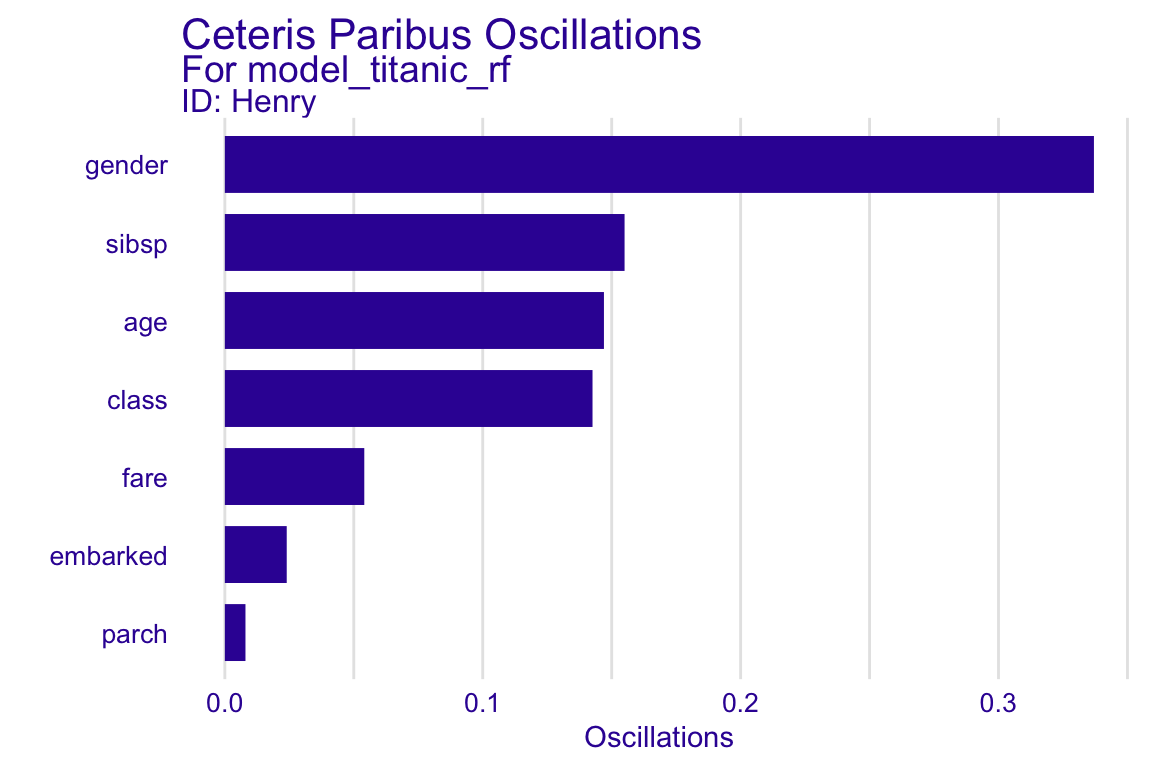
\includegraphics{PM_VEE_files/figure-latex/unnamed-chunk-5-1.pdf}

\hypertarget{breakDown}{%
\section{Variable attributions}\label{breakDown}}

In the Section \ref{variableAttributionMethods} we introduced a method
for calculation of variable attributions for linear models. This method
is accurate, based directly on the structure of the model. But for most
popular machine learning models we cannot assume that they are linear
nor even additive.

\hypertarget{intuition-1}{%
\subsection{Intuition}\label{intuition-1}}

For any model we may repeat the intuition presented in Section
\ref{variableAttributionMethods} to calculate variable contribution as
shifts in expected model response after conditioning over consecutive
variables. This intuition is presented in Figure \ref{BDPrice4}.

Panel A shows distribution of model responses. The row
\texttt{all\ data} shows the model response of the original dataset. The
red dot stands for average is is an estimate of expencted model response
\(E [f(x)]\).

Since we want to calculate effects of particular values of selected
variables we then condition over these variables in a sequential manner.
The next row in panel A corresponds to average model prediction for
observations with variable \texttt{surface} fixed to value \texttt{35}.
The next for corresponds to average model prediction with variables
\texttt{surface} set to \texttt{35} and \texttt{floor} set to
\texttt{1}, and so on. The top row corresponds to model response for
\(x^*\).

Black lines in the panel A show how prediction for a single point
changes after coordinate \(i\) is repaced by the \(x^*_i\). But finaly
we are not interestes in particular changes, not even in distributions
but only in averages - expected model responses.

The most minimal form that shows important information is presented in
the panel C. Positive values are presented with green bars while
negative differences are marked with yellow bar. They sum up to final
model prediction, which is denoted by a grey bar in this example.

\begin{figure}

{\centering 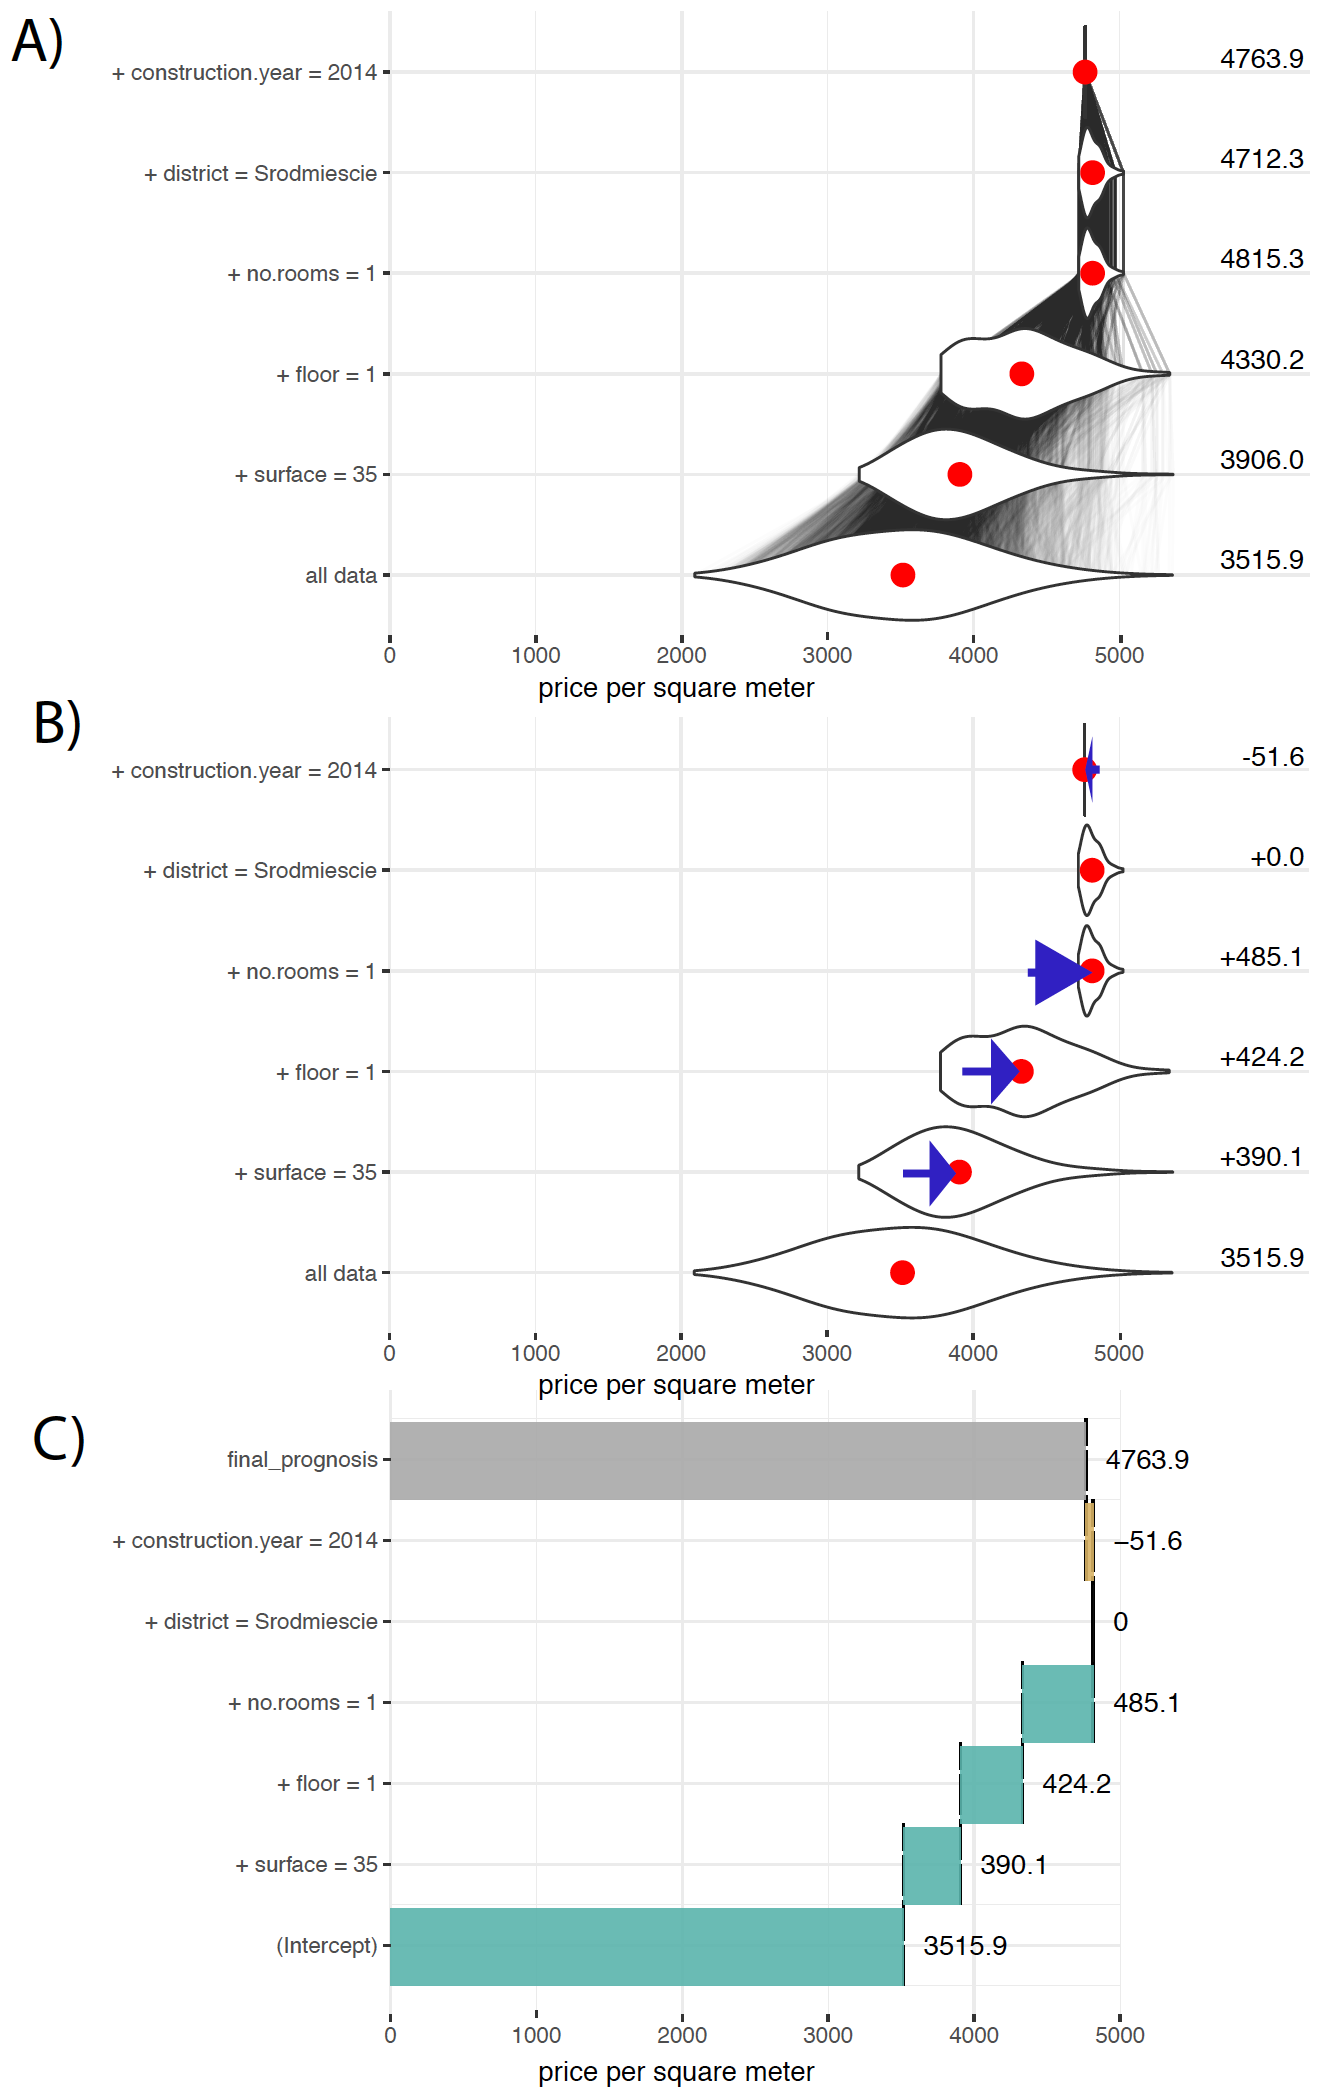
\includegraphics[width=0.7\linewidth]{figure/bd_price_4} 

}

\caption{(fig:BDPrice4) Break Down Plots show how variables move the model prediction from population average to the model prognosis for a single observation. A) The last row shows distribution of model predictions. Next rows show conditional distributions, every row a new variable is added to conditioning. The first row shows model prediction for a single point. Red dots stand for averages. B) Blue arrows shows how the average conditional response change, these values are variables contributions. C) Only variable contributions are presented. }\label{fig:BDPrice4}
\end{figure}

\hypertarget{method-1}{%
\subsection{Method}\label{method-1}}

Again, let \(v(f, x^*, i)\) stands for the contribution of variable
\(x_i\) on prediction of model \(f()\) in point \(x^*\).

We expect that such contribution will sum up to the model prediction in
a given point (property called \emph{local accuracy}), so \[
f(x^*) = baseline + \sum_{i=1}^p v(f, x^*, i)
\] where \(baseline\) stands for average model response.

Note that the equation above may be rewritten as

\[
E [f(X)|X_1 = x_1^*, \ldots, X+p = x_p^*] = E[f(X)] + \sum_{i=1}^p v(f, x^*, i)
\] what leads to quite natural proposition for \(v(f, x^*_i, i)\), such
as

\[
v(f, x^*_i, i) = E [f(X) | X_1 = x_1^*, \ldots, X_i = x_i^*] - E [f(X) | X_1 = x_1^*, \ldots, X_{i-1} = x_{i-1}^*] 
\] In other words the contribution of variable \(i\) is the difference
between expected model response conditioned on first \(i\) variables
minus the model response conditioned on first \(i-1\) variables.

Such proposition fulfills the \emph{local accuracy} condition, but
unfortunatelly variable contributions depends on the ordering of
variables.

\begin{figure}

{\centering 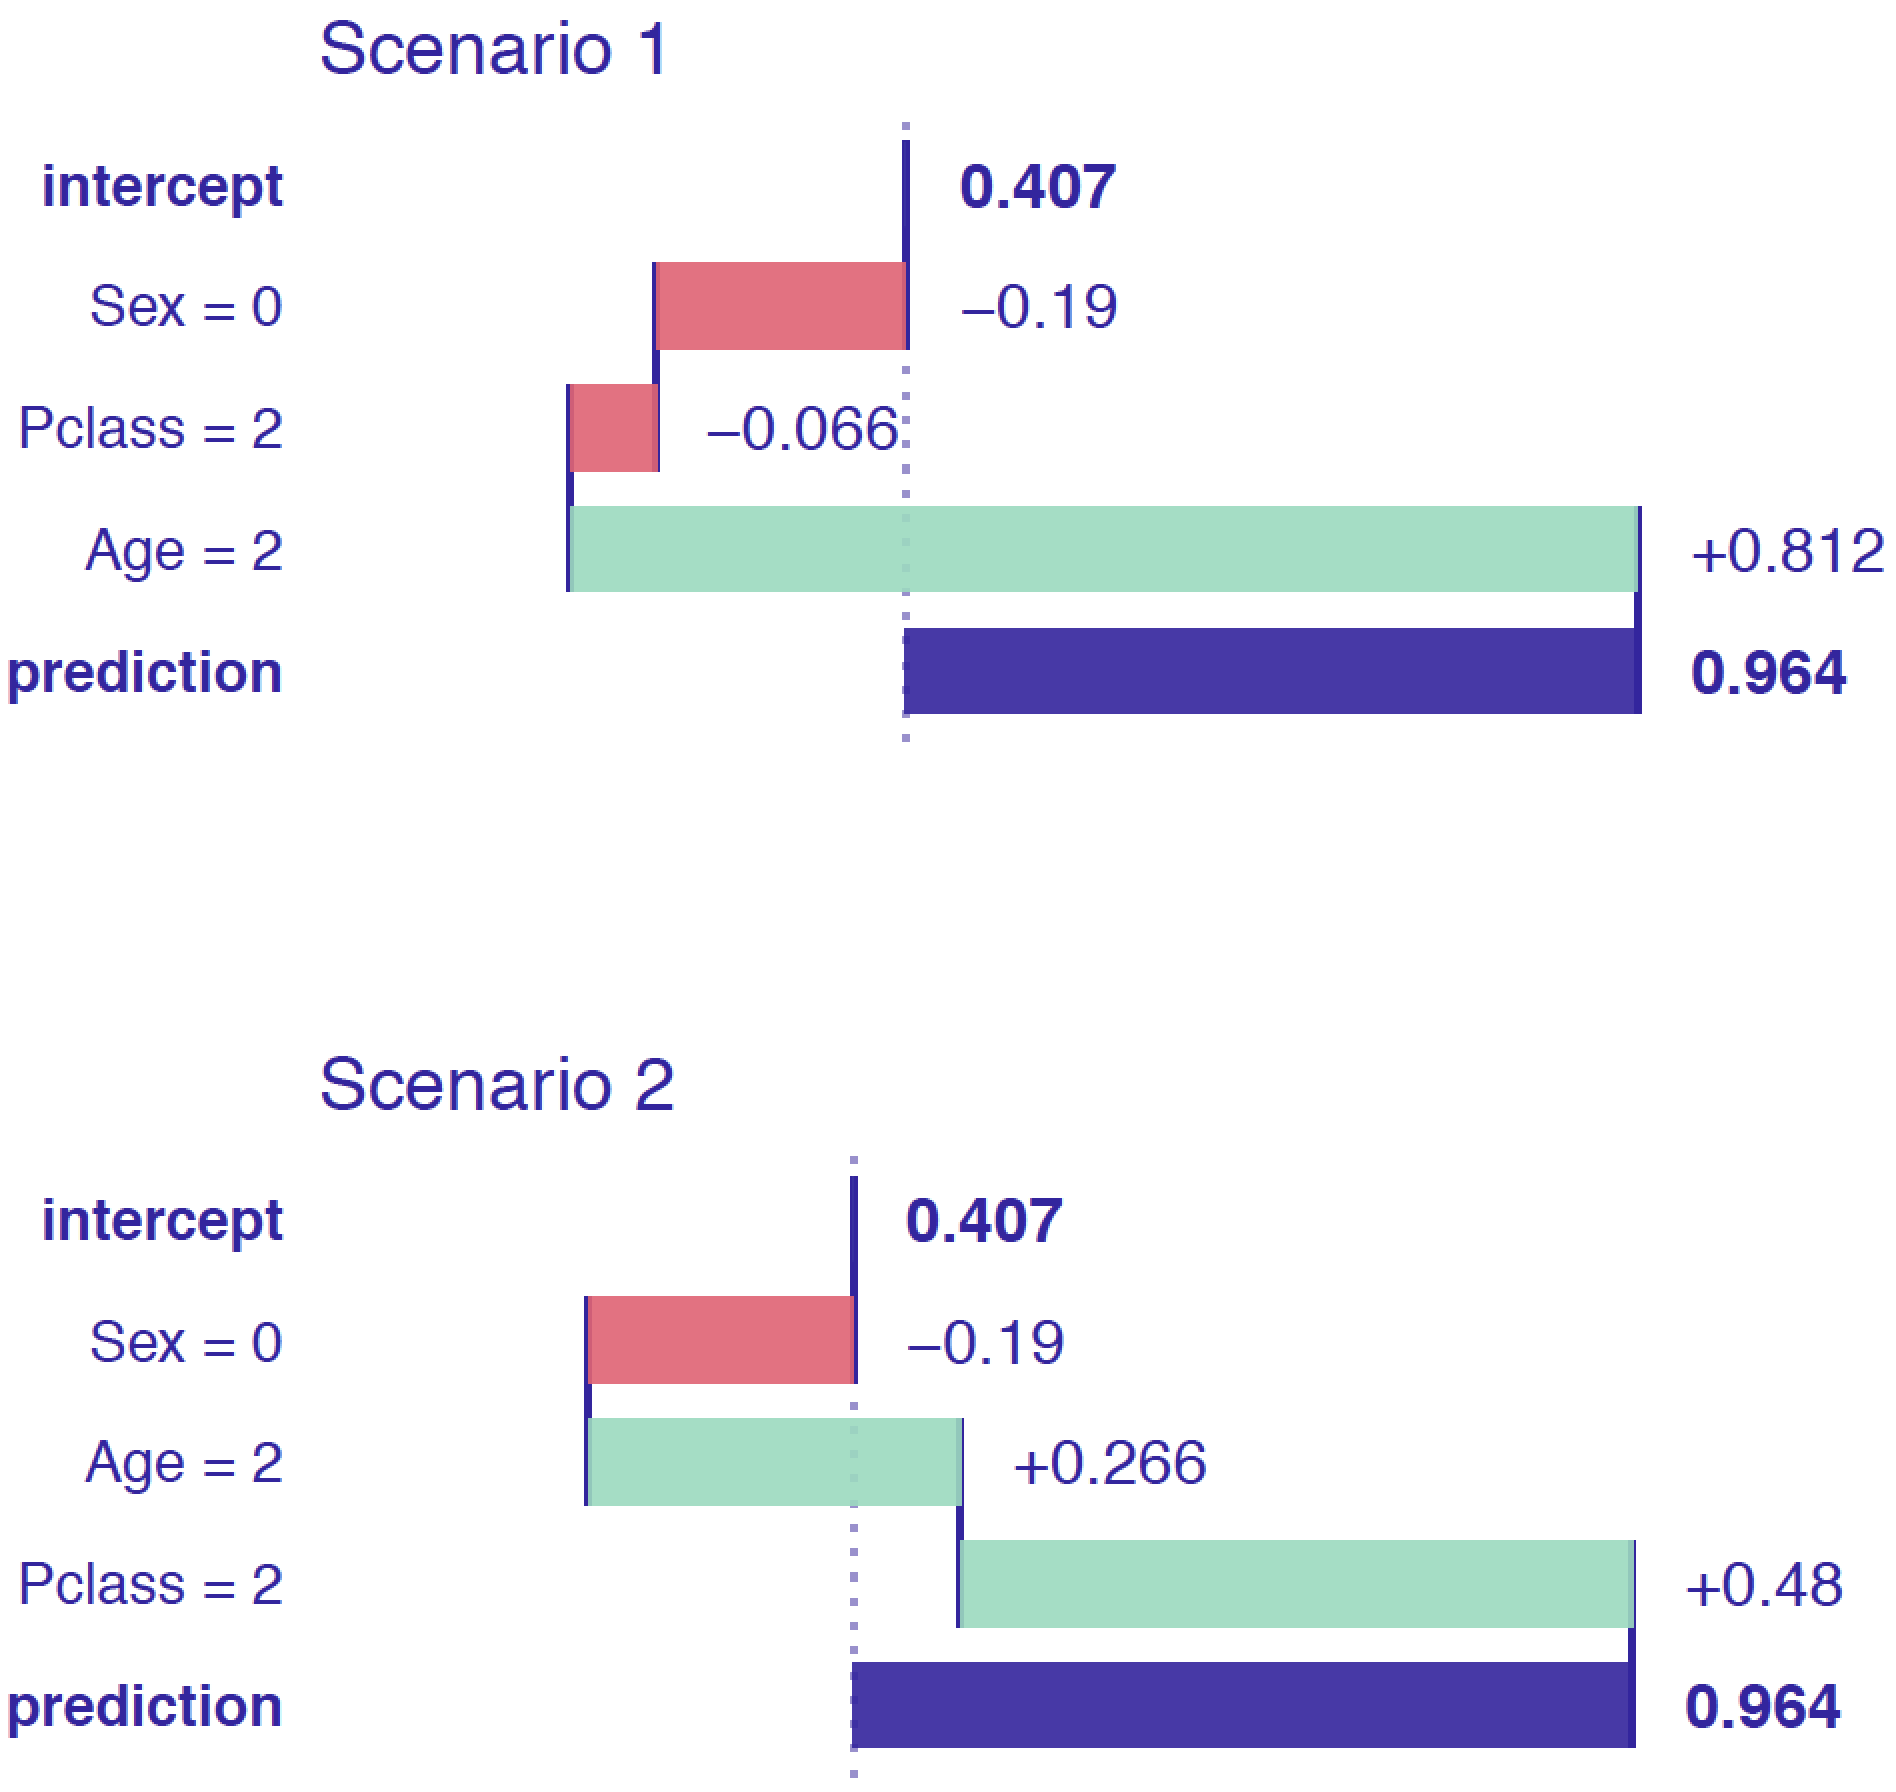
\includegraphics[width=1\linewidth]{figure/ordering} 

}

\caption{(fig:ordering) Two different paths between average model prediction and the model prediction for a selected observation. Black dots stand for conditional average, red arrows stands for changes between conditional averages.}\label{fig:ordering}
\end{figure}

See for example Figure \ref{fig:ordering}. In the first ordering the
contribution of variable \texttt{age} is calculated as 0.01, while in
the second the contribution is calculated as 0.13. Such differences are
related to the lack of additivness of the model \(f()\). Propositions
presented in next two sections present different solutions for this
problem.

The approach for variable attribution presented in the Section
\ref{modelAgnosticAttribution} has the property of \emph{local
accuracy}, but variable contributions depends on the variable ordering.

The easiest way to solve this problem is to use two-step procedure. In
the first step variables are ordered and in the second step the
consecutive conditioning is applied to ordered variables.

First step of this algorithm is to determine the order of variables for
conditioning. It seems to be reasonable to include first variables that
are likely to be most important, leaving the noise variables at the end.
This leads to order based on following scores

\[
score(f, x^*, i) = \left| E [f(X)] - E [f(X)|X_i = x^*_i] \right|
\] Note, that the absolute value is needed as variable contributions can
be both positive and negative.

Once the ordering is determined in the second step variable
contributions are calculated as

\[
v(f, x^*_i, i) = E [f(X) | X_{I \cup \{i\}} = x_{I \cup \{i\}}^*] - E [f(X) | X_{I} = x_{I}^*] 
\] where \(I\) is the set of variables that have scores smaller than
score for variable \(i\).

\[
I = \{j: score(f, x^*, j) < score(f, x^*, i)\}
\]

The time complexity of the first step id \(O(p)\) where \(p\) is the
number of variables and the time complexity of the second step is also
\(O(p)\).

\hypertarget{example-hire-or-fire}{%
\subsection{Example: Hire or Fire?}\label{example-hire-or-fire}}

Let us consider a random forest model created for HR data. The average
model response is \(\bar f(x) = 0.385586\). For a selected observation
\(x^*\) the table below presents scores for particular variables.

\begin{longtable}[]{@{}lrr@{}}
\toprule
& Ei f(X) & scorei\tabularnewline
\midrule
\endhead
hours & 0.616200 & 0.230614\tabularnewline
salary & 0.225528 & 0.160058\tabularnewline
evaluation & 0.430994 & 0.045408\tabularnewline
age & 0.364258 & 0.021328\tabularnewline
gender & 0.391060 & 0.005474\tabularnewline
\bottomrule
\end{longtable}

Once we determine the order we can calculate sequential contributions

\begin{longtable}[]{@{}lrr@{}}
\toprule
variable & cumulative & contribution\tabularnewline
\midrule
\endhead
(Intercept) & 0.385586 & 0.385586\tabularnewline
* hours = 42 & 0.616200 & 0.230614\tabularnewline
* salary = 2 & 0.400206 & -0.215994\tabularnewline
* evaluation = 2 & 0.405776 & 0.005570\tabularnewline
* age = 58 & 0.497314 & 0.091538\tabularnewline
* gender = male & 0.778000 & 0.280686\tabularnewline
final\_prognosis & 0.778000 & 0.778000\tabularnewline
\bottomrule
\end{longtable}

\hypertarget{pros-and-cons-1}{%
\subsection{Pros and cons}\label{pros-and-cons-1}}

Break Down approach is model agnostic, can be applied to any predictive
model that returns a single number. It leads to additive variable
attribution. Below we summarize key strengths and weaknesses of this
approach.

\textbf{Pros}

\begin{itemize}
\tightlist
\item
  Break Down Plots are easy to understand and decipher.
\item
  Break Down Plots are compact; many variables may be presented in a
  small space.
\item
  Break Down Plots are model agnostic yet they reduce to intuitive
  interpretation for linear Gaussian and generalized models.
\item
  Complexity of Break Down Algorithm is linear in respect to the number
  of variables.
\end{itemize}

\textbf{Cons}

\begin{itemize}
\tightlist
\item
  If the model is non-additive then showing only additive contributions
  may be misleading.
\item
  Selection of the ordering based on scores is subjective. Different
  orderings may lead to different contributions.
\item
  For large number of variables the Break Down Plot may be messy with
  many variables having small contributions.
\end{itemize}

\hypertarget{code-snippets-for-r}{%
\subsection{Code snippets for R}\label{code-snippets-for-r}}

In this section we present key features of the \texttt{breakDown2}
package for R \citep{R-breakDown}. This package covers all features
presented in this chapter. It is available on CRAN and GitHub. Find more
examples at the website of this package
\texttt{https://pbiecek.github.io/breakDown2/}.

\textbf{Model preparation}

In this section we will present an example based on the \texttt{HR}
dataset and Random Forest model \citep{R-randomForest}. See the Section
\ref{HRdataset} for more details.

\begin{Shaded}
\begin{Highlighting}[]
\KeywordTok{library}\NormalTok{(}\StringTok{"DALEX2"}\NormalTok{)}
\KeywordTok{library}\NormalTok{(}\StringTok{"randomForest"}\NormalTok{)}
\NormalTok{model <-}\StringTok{ }\KeywordTok{randomForest}\NormalTok{(status }\OperatorTok{~}\StringTok{ }\NormalTok{gender }\OperatorTok{+}\StringTok{ }\NormalTok{age }\OperatorTok{+}\StringTok{ }\NormalTok{hours }\OperatorTok{+}\StringTok{ }\NormalTok{evaluation }\OperatorTok{+}\StringTok{ }\NormalTok{salary, }\DataTypeTok{data =}\NormalTok{ HR)}
\NormalTok{model}
\end{Highlighting}
\end{Shaded}

\begin{verbatim}
## 
## Call:
##  randomForest(formula = status ~ gender + age + hours + evaluation +      salary, data = HR) 
##                Type of random forest: classification
##                      Number of trees: 500
## No. of variables tried at each split: 2
## 
##         OOB estimate of  error rate: 27.4%
## Confusion matrix:
##          fired   ok promoted class.error
## fired     2276  378      201   0.2028021
## ok         534 1243      444   0.4403422
## promoted   202  391     2178   0.2140022
\end{verbatim}

Model exploration with the \texttt{breakDown2} package is performed in
three steps.

\textbf{1. Create an explainer - wrapper around model and validation
data.}

Since all other functions work in a model agnostic fashion, first we
need to define a wrapper around the model. Here we are using the
\texttt{explain()} function from \texttt{DALEX2} package
\citep{R-DALEX}.

\begin{Shaded}
\begin{Highlighting}[]
\NormalTok{explainer_rf <-}\StringTok{ }\KeywordTok{explain}\NormalTok{(model,}
                 \DataTypeTok{data =}\NormalTok{ HR,}
                 \DataTypeTok{y =}\NormalTok{ HR}\OperatorTok{$}\NormalTok{status)}
\end{Highlighting}
\end{Shaded}

\textbf{2. Select an observation of interest.}

Break Down Plots decompose model prediction around a single observation.
Let's construct a data frame with corresponding values.

\begin{Shaded}
\begin{Highlighting}[]
\NormalTok{new_observation <-}\StringTok{ }\KeywordTok{data.frame}\NormalTok{(}\DataTypeTok{gender =} \KeywordTok{factor}\NormalTok{(}\StringTok{"male"}\NormalTok{, }\DataTypeTok{levels =} \KeywordTok{c}\NormalTok{(}\StringTok{"male"}\NormalTok{, }\StringTok{"female"}\NormalTok{)),}
                      \DataTypeTok{age =} \FloatTok{57.7}\NormalTok{,}
                      \DataTypeTok{hours =} \FloatTok{42.3}\NormalTok{,}
                      \DataTypeTok{evaluation =} \DecValTok{2}\NormalTok{,}
                      \DataTypeTok{salary =} \DecValTok{2}\NormalTok{)}

\KeywordTok{predict}\NormalTok{(model, new_observation, }\DataTypeTok{type =} \StringTok{"prob"}\NormalTok{)}
\end{Highlighting}
\end{Shaded}

\begin{verbatim}
##   fired    ok promoted
## 1 0.762 0.238        0
## attr(,"class")
## [1] "matrix" "votes"
\end{verbatim}

\textbf{3. Calculate Break Down decomposition}

The \texttt{local\_attributions()} function calculates Break Down
contributions for a selected model around a selected observation.

The result from \texttt{local\_attributions()} function is a data frame
with variable attributions.

\begin{Shaded}
\begin{Highlighting}[]
\KeywordTok{library}\NormalTok{(}\StringTok{"breakDown2"}\NormalTok{)}
\NormalTok{bd_rf <-}\StringTok{ }\KeywordTok{local_attributions}\NormalTok{(explainer_rf,}
\NormalTok{                 new_observation,}
                 \DataTypeTok{keep_distributions =} \OtherTok{TRUE}\NormalTok{)}

\NormalTok{bd_rf}
\end{Highlighting}
\end{Shaded}

\begin{verbatim}
##                                         contribution
## randomForest.fired: baseline                   0.375
## randomForest.fired: * hours = 42               0.236
## randomForest.fired: * evaluation = 2           0.060
## randomForest.fired: * salary = 2              -0.258
## randomForest.fired: * age = 58                 0.083
## randomForest.fired: * gender = male            0.266
## randomForest.fired: prediction                 0.762
## randomForest.ok: baseline                      0.274
## randomForest.ok: * hours = 42                 -0.047
## randomForest.ok: * evaluation = 2              0.095
## randomForest.ok: * salary = 2                  0.257
## randomForest.ok: * age = 58                   -0.078
## randomForest.ok: * gender = male              -0.264
## randomForest.ok: prediction                    0.238
## randomForest.promoted: baseline                0.350
## randomForest.promoted: * hours = 42           -0.189
## randomForest.promoted: * evaluation = 2       -0.156
## randomForest.promoted: * salary = 2            0.001
## randomForest.promoted: * age = 58             -0.005
## randomForest.promoted: * gender = male        -0.002
## randomForest.promoted: prediction              0.000
## baseline:  0
\end{verbatim}

The generic \texttt{plot()} function creates a Break Down plots.

\begin{Shaded}
\begin{Highlighting}[]
\KeywordTok{plot}\NormalTok{(bd_rf) }
\end{Highlighting}
\end{Shaded}

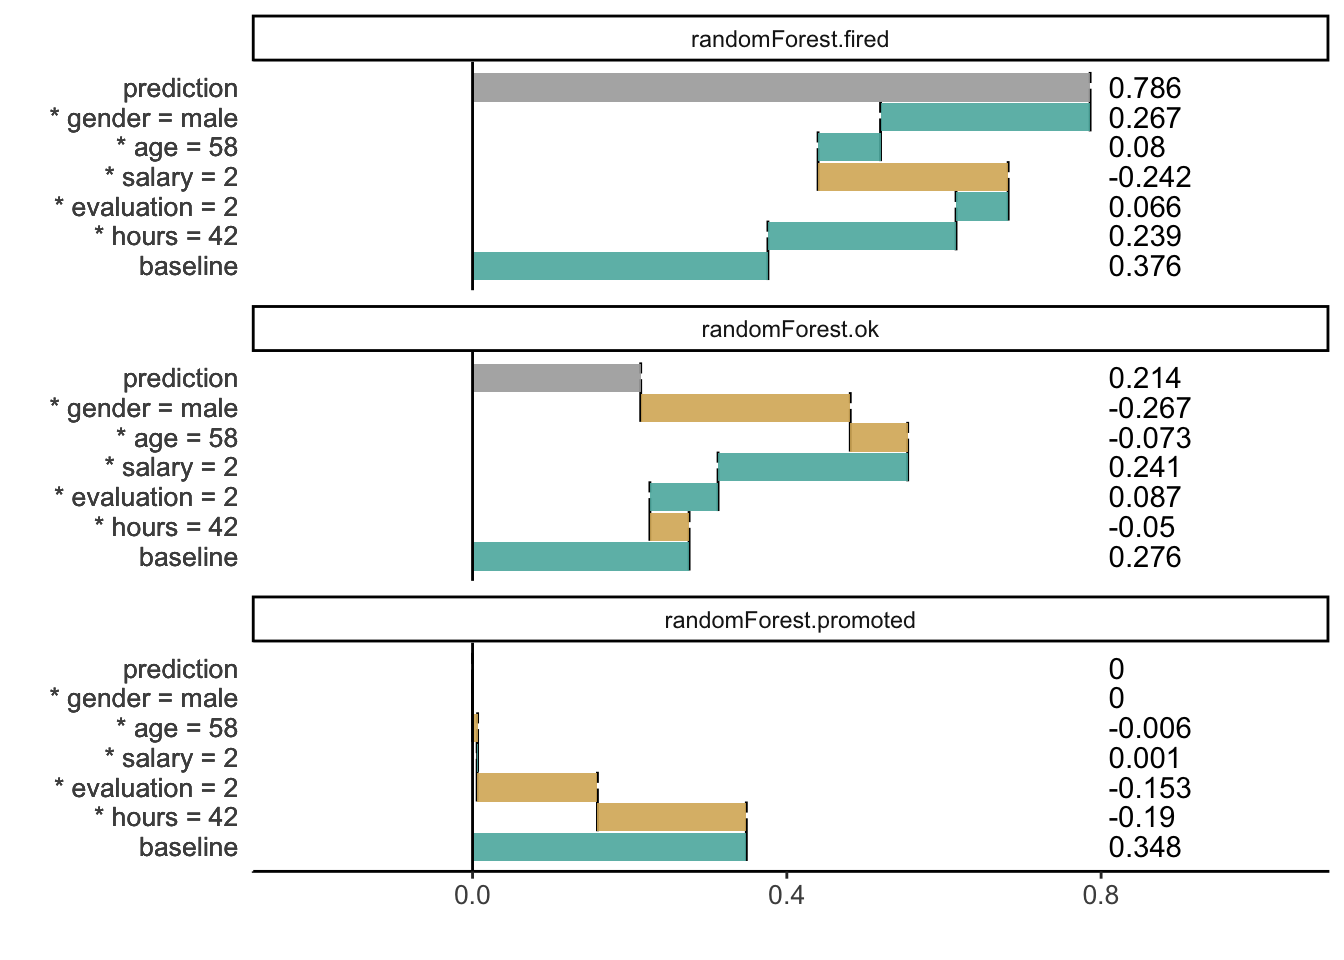
\includegraphics{PM_VEE_files/figure-latex/unnamed-chunk-10-1.pdf}

Add the \texttt{plot\_distributions\ =\ TRUE} argument to enrich model
response with additional information.

\begin{Shaded}
\begin{Highlighting}[]
\KeywordTok{plot}\NormalTok{(bd_rf, }\DataTypeTok{plot_distributions =} \OtherTok{TRUE}\NormalTok{) }
\end{Highlighting}
\end{Shaded}

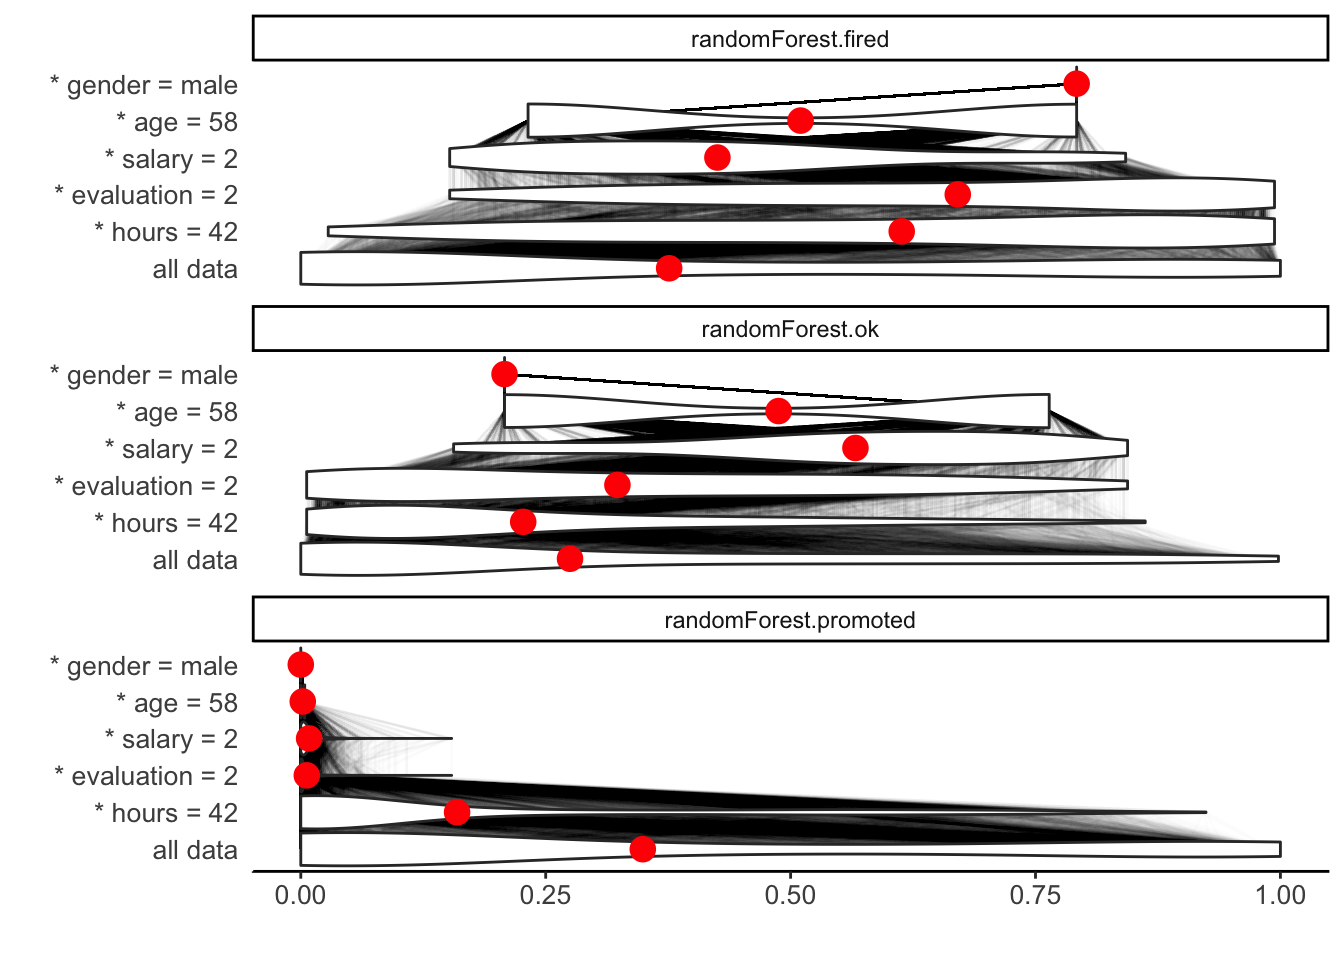
\includegraphics{PM_VEE_files/figure-latex/unnamed-chunk-11-1.pdf}

\hypertarget{variable-attribution-with-interactions}{%
\section{Variable attribution with
interactions}\label{variable-attribution-with-interactions}}

In the Section \ref{breakDown} we presented model agnostic approach for
additive decomposition of a model prediction for a single observation.

For non-additive models the variables contributions depend on values of
other variables.

In this section we present an algorithm that identifies interactions
between pairs of variables and include such interactions in variable
decomposition plots. Here we present an algorithm for pairs of
variables, but it can be easily generalized to larger number of
variables.

\hypertarget{intuition-2}{%
\subsection{Intuition}\label{intuition-2}}

The key idea here is to identify interactions between variables. This
can be done in two steps.

\begin{enumerate}
\def\labelenumi{\arabic{enumi}.}
\tightlist
\item
  First we determine variable contributions for each variable
  independently.
\item
  Second, we calculate effect for pair of variables. If this effect is
  different than the sum of consecutive variables then it may be an
  interaction.
\end{enumerate}

TODO: easy example for interaction

\hypertarget{method-2}{%
\subsection{Method}\label{method-2}}

This algorithm is also composed out of two steps. In the first step
variables and pairs of variables are ordered in terms of their
importance, while in the second step the consecutive conditioning is
applied to ordered variables.

To determine an importance of variables and pairs of variables following
scores are being calculated.

For a single variable

\[
score_1(f, x^*, i) = \left| E [f(X)|X_i = x^*_i]  - E [f(X)]\right|
\] For pairs of variables

\[
score_2(f, x^*, (i,j)) = \left| E [f(X)|X_i = x^*_i, X_j = x^*_j] - E [f(X)|X_i = x^*_i] - E [f(X)| X_j = x^*_j]+ E [f(X)] \right|
\] Note that this is equivalent to

\[
score_2(f, x^*, (i,j)) = \left| E [f(X)|X_i = x^*_i, X_j = x^*_j] - score_1 (f, x^*, i) - score_1 (f, x^*, j) + baseline \right|
\] In other words the \(score_1(f, x^*, i)\) measures how much the
average model response changes if variable \(x_i\) is set to \(x_i^*\),
which is some index of local variable importance. On the other hand the
\(score_2(f, x^*, (i,j))\) measures how much the change is different
than additive composition of changes for \(x_i\) and \(x_j\), which is
some index of local interaction importance.

Note, that for additive models \(score_2(f, x^*, (i,j))\) shall be close
to zero. So the larger is this value the larger deviation from
additivness.

The second step of the algorithm is the sequential conditioning. In this
version in every new step we condition on a single variable of pair of
variables in an order determined by \(score_1\) and \(score_2\).

The complexity of the first step id \(O(p^2)\) where \(p\) stands for
the number of variables. The complexity of the second step is \(O(p)\).

\hypertarget{example-hire-or-fire-1}{%
\subsection{Example: Hire or Fire?}\label{example-hire-or-fire-1}}

Again, let us consider a HR dataset. The table below shows \(score_1\)
and \(score_2\) calculated for consecutive variables.

\begin{longtable}[]{@{}lrrr@{}}
\toprule
& Ei f(X) & score1 & score2\tabularnewline
\midrule
\endhead
hours & 0.616200 & 0.230614 &\tabularnewline
salary & 0.225528 & -0.160058 &\tabularnewline
age:gender & 0.516392 & & 0.146660\tabularnewline
salary:age & 0.266226 & & 0.062026\tabularnewline
salary:hours & 0.400206 & & -0.055936\tabularnewline
evaluation & 0.430994 & 0.045408 &\tabularnewline
hours:age & 0.635662 & & 0.040790\tabularnewline
salary:evaluation & 0.238126 & & -0.032810\tabularnewline
age & 0.364258 & -0.021328 &\tabularnewline
evaluation:hours & 0.677798 & & 0.016190\tabularnewline
salary:gender & 0.223292 & & -0.007710\tabularnewline
evaluation:age & 0.415688 & & 0.006022\tabularnewline
gender & 0.391060 & 0.005474 &\tabularnewline
hours:gender & 0.626478 & & 0.004804\tabularnewline
evaluation:gender & 0.433814 & & -0.002654\tabularnewline
\bottomrule
\end{longtable}

Once we determined the order, we can calculate sequential conditionings.
In the first step we condition over variable \texttt{hours}, then over
\texttt{salary}. The third position is occupied by interaction between
\texttt{age:gender} thus we add both variables to the conditioning

\begin{longtable}[]{@{}lrr@{}}
\toprule
variable & cumulative & contribution\tabularnewline
\midrule
\endhead
(Intercept) & 0.385586 & 0.385586\tabularnewline
* hours = 42 & 0.616200 & 0.230614\tabularnewline
* salary = 2 & 0.400206 & -0.215994\tabularnewline
* age:gender = 58:male & 0.796856 & 0.396650\tabularnewline
* evaluation = 2 & 0.778000 & -0.018856\tabularnewline
final\_prognosis & 0.778000 & 0.778000\tabularnewline
\bottomrule
\end{longtable}

\hypertarget{break-down-plots}{%
\subsection{Break Down Plots}\label{break-down-plots}}

Break Down Plots for interactions are similar in structure as plots for
single variables. The only difference is that in some rows pair of
variable is listed in a single row. See an example in Figure
\ref{BDPrice4}.

\begin{figure}

{\centering 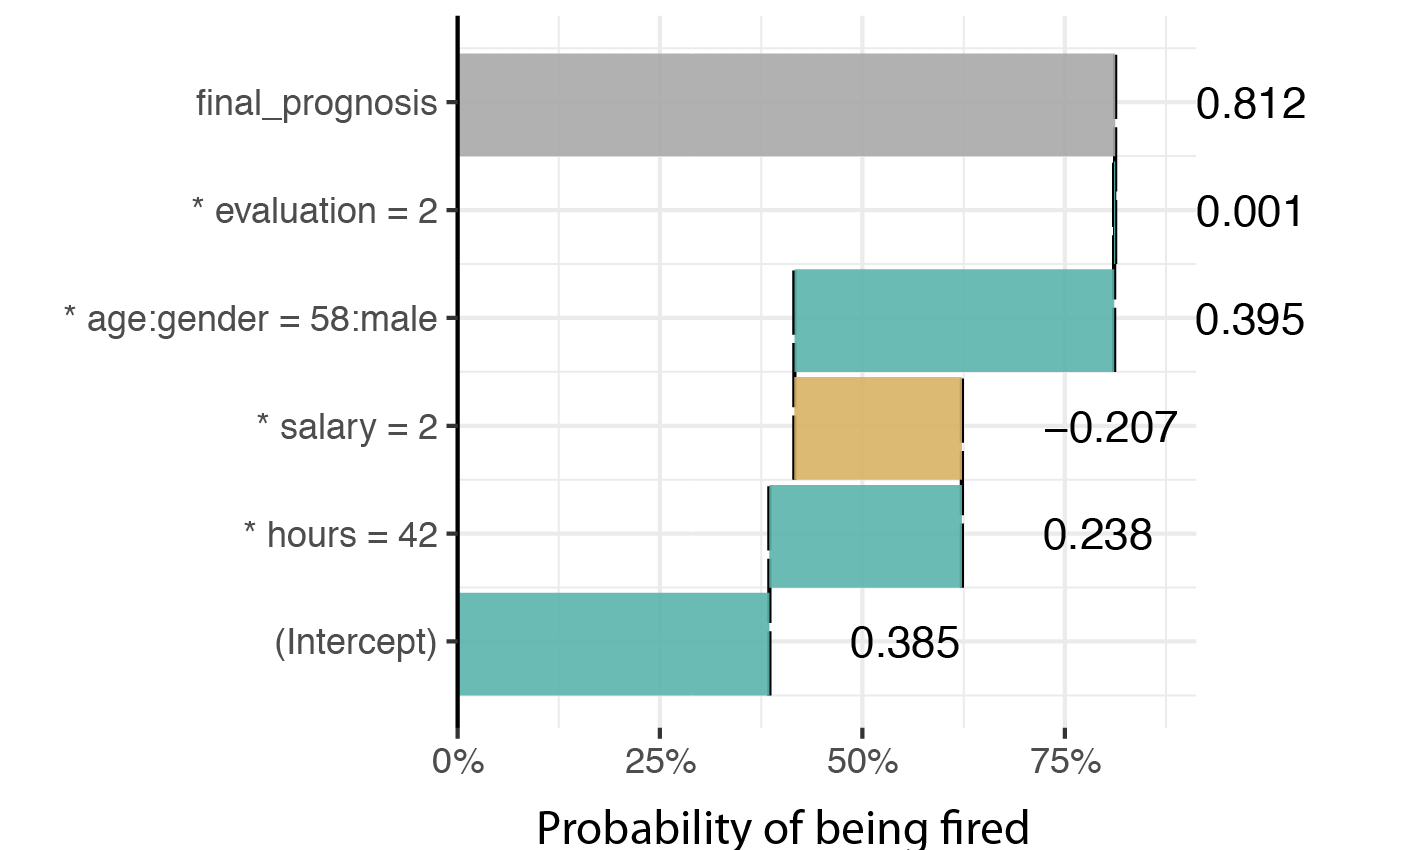
\includegraphics[width=0.7\linewidth]{figure/bd_inter_1} 

}

\caption{(fig:bdInter1) Break Down Plot for variable attrbution with interactions }\label{fig:bdInter1}
\end{figure}

\hypertarget{pros-and-cons-2}{%
\subsection{Pros and cons}\label{pros-and-cons-2}}

Break Down for interactions shares many features of Break Down for
single variables. Below we summarize unique strengths and weaknesses of
this approach.

\textbf{Pros}

\begin{itemize}
\tightlist
\item
  If interactions are present in the model, then additive contributions
  may be misleading. In such case the identification of interactions
  leads to better explanations.
\item
  Complexity of Break Down Algorithm is quadratic, what is not that bad
  if number of features is small or moderate.
\end{itemize}

\textbf{Cons}

\begin{itemize}
\tightlist
\item
  For large number of variables, the consideration of all interactions
  is both time consuming and sensitive to noise as the number of
  \(score_2\) scores grow faster than number of \(score_1\).
\end{itemize}

\hypertarget{code-snippets-for-r-1}{%
\subsection{Code snippets for R}\label{code-snippets-for-r-1}}

The algorithm for Break Down for Interactions is also implemented in the
\texttt{local\_interactions} function from \texttt{breakDown2} package.

\textbf{Model preparation}

First a model needs to be trained.

\begin{Shaded}
\begin{Highlighting}[]
\KeywordTok{library}\NormalTok{(}\StringTok{"DALEX2"}\NormalTok{)}
\KeywordTok{library}\NormalTok{(}\StringTok{"randomForest"}\NormalTok{)}
\NormalTok{model <-}\StringTok{ }\KeywordTok{randomForest}\NormalTok{(status }\OperatorTok{~}\StringTok{ }\NormalTok{gender }\OperatorTok{+}\StringTok{ }\NormalTok{age }\OperatorTok{+}\StringTok{ }\NormalTok{hours }\OperatorTok{+}\StringTok{ }\NormalTok{evaluation }\OperatorTok{+}\StringTok{ }\NormalTok{salary, }\DataTypeTok{data =}\NormalTok{ HR)}
\NormalTok{model}
\end{Highlighting}
\end{Shaded}

\begin{verbatim}
## 
## Call:
##  randomForest(formula = status ~ gender + age + hours + evaluation +      salary, data = HR) 
##                Type of random forest: classification
##                      Number of trees: 500
## No. of variables tried at each split: 2
## 
##         OOB estimate of  error rate: 27.39%
## Confusion matrix:
##          fired   ok promoted class.error
## fired     2269  399      187   0.2052539
## ok         535 1250      436   0.4371905
## promoted   211  381     2179   0.2136413
\end{verbatim}

Model exploration with the \texttt{breakDown2} package is performed in
three steps.

\textbf{1. Create an explainer - wrapper around model and validation
data.}

Since all other functions work in a model agnostic fashion, first we
need to define a wrapper around the model. Here we are using the
\texttt{explain()} function from \texttt{DALEX} package.

\begin{Shaded}
\begin{Highlighting}[]
\NormalTok{explainer_rf <-}\StringTok{ }\KeywordTok{explain}\NormalTok{(model,}
                 \DataTypeTok{data =}\NormalTok{ HR,}
                 \DataTypeTok{y =}\NormalTok{ HR}\OperatorTok{$}\NormalTok{status)}
\end{Highlighting}
\end{Shaded}

\textbf{2. Select an observation of interest.}

Break Down Plots decompose model prediction around a single observation.
Let's construct a data frame with corresponding values.

\begin{Shaded}
\begin{Highlighting}[]
\NormalTok{new_observation <-}\StringTok{ }\KeywordTok{data.frame}\NormalTok{(}\DataTypeTok{gender =} \KeywordTok{factor}\NormalTok{(}\StringTok{"male"}\NormalTok{, }\DataTypeTok{levels =} \KeywordTok{c}\NormalTok{(}\StringTok{"male"}\NormalTok{, }\StringTok{"female"}\NormalTok{)),}
                      \DataTypeTok{age =} \FloatTok{57.7}\NormalTok{,}
                      \DataTypeTok{hours =} \FloatTok{42.3}\NormalTok{,}
                      \DataTypeTok{evaluation =} \DecValTok{2}\NormalTok{,}
                      \DataTypeTok{salary =} \DecValTok{2}\NormalTok{)}

\KeywordTok{predict}\NormalTok{(model, new_observation, }\DataTypeTok{type =} \StringTok{"prob"}\NormalTok{)}
\end{Highlighting}
\end{Shaded}

\begin{verbatim}
##   fired   ok promoted
## 1 0.788 0.21    0.002
## attr(,"class")
## [1] "matrix" "votes"
\end{verbatim}

\textbf{3. Calculate Break Down decomposition}

The \texttt{local\_interactions()} function calculates Break Down
contributions for a selected model around a selected observation.

The result from \texttt{local\_interactions()} function is a data frame
with variable attributions.

\begin{Shaded}
\begin{Highlighting}[]
\KeywordTok{library}\NormalTok{(}\StringTok{"breakDown2"}\NormalTok{)}
\NormalTok{bd_rf <-}\StringTok{ }\KeywordTok{local_interactions}\NormalTok{(explainer_rf,}
\NormalTok{                 new_observation)}

\NormalTok{bd_rf}
\end{Highlighting}
\end{Shaded}

\begin{verbatim}
##                                               contribution
## randomForest.fired: baseline                         0.377
## randomForest.fired: * hours = 42                     0.238
## randomForest.fired: * salary = 2                    -0.212
## randomForest.fired: * age:gender = 58:male           0.382
## randomForest.fired: * evaluation = 2                 0.004
## randomForest.fired: prediction                       0.788
## randomForest.ok: baseline                            0.275
## randomForest.ok: * evaluation = 2                    0.137
## randomForest.ok: * salary = 2                        0.154
## randomForest.ok: * age:gender = 58:male             -0.279
## randomForest.ok: * hours = 42                       -0.076
## randomForest.ok: prediction                          0.210
## randomForest.promoted: baseline                      0.349
## randomForest.promoted: * hours = 42                 -0.190
## randomForest.promoted: * evaluation = 2             -0.152
## randomForest.promoted: * age:gender = 58:male       -0.005
## randomForest.promoted: * salary = 2                  0.001
## randomForest.promoted: prediction                    0.002
## baseline:  0
\end{verbatim}

The generic \texttt{plot()} function creates a Break Down plots.

\begin{Shaded}
\begin{Highlighting}[]
\KeywordTok{plot}\NormalTok{(bd_rf) }
\end{Highlighting}
\end{Shaded}

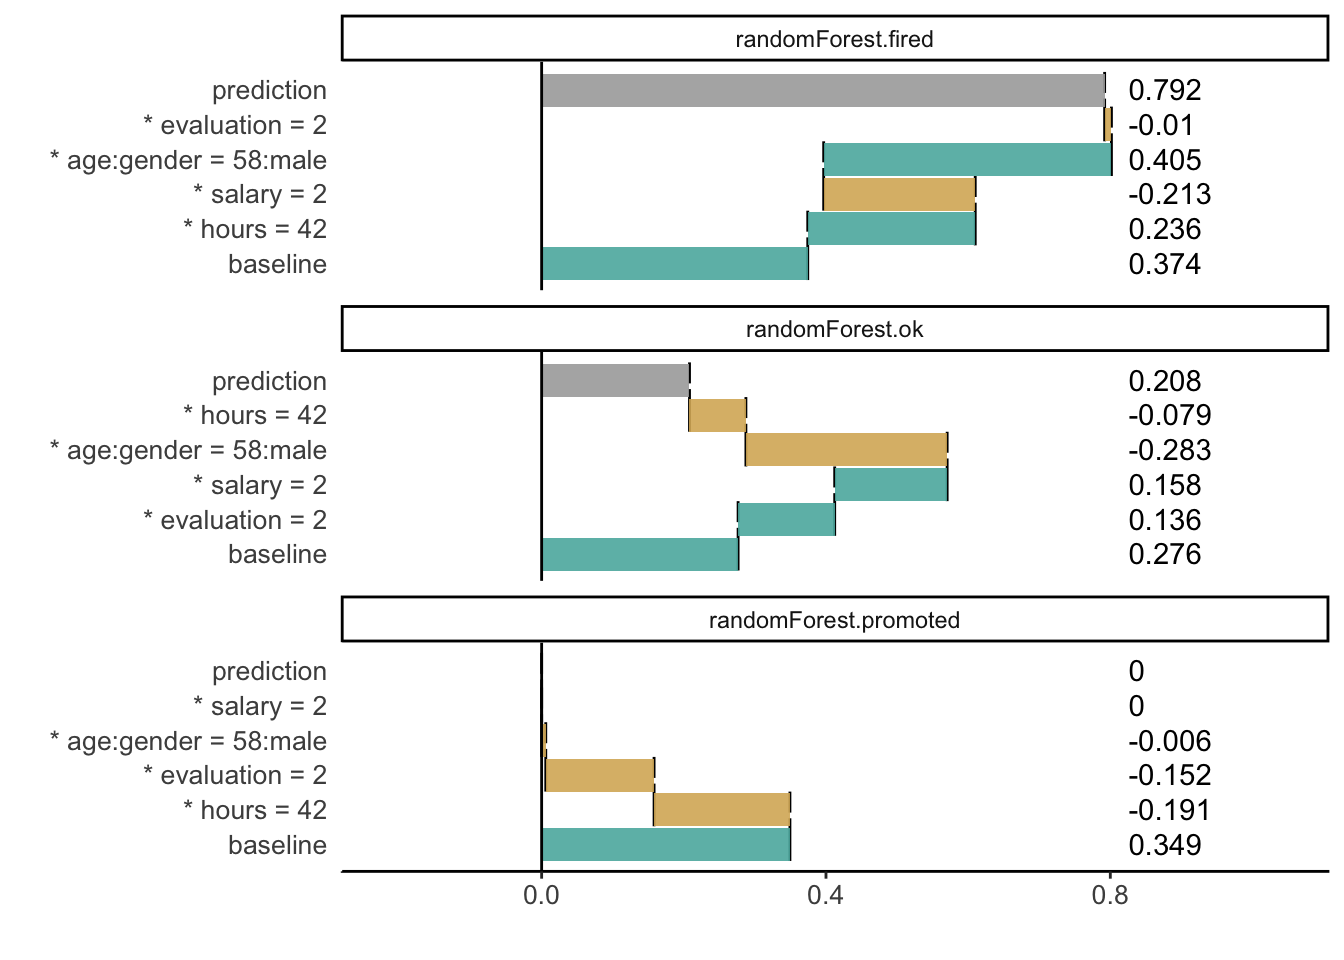
\includegraphics{PM_VEE_files/figure-latex/unnamed-chunk-16-1.pdf}

\hypertarget{shapley}{%
\section{Average variable attributions}\label{shapley}}

In the Section \ref{modelAgnosticAttribution} we show the problem
related to the ordering of variables. In the Section \ref{breakDown} we
show an approach in which the ordering was determined based on single
step assessment of variable importance.

In this section we introduce other, very popular approach for additive
variable attribution. The problem of contributions that depends on the
variable ordering is solved by averaging over all possible orderings.

This method is motivated with results in cooperative game theory and was
first introduced in \citep{Strumbelj2014}. Wide adoption of this method
comes with a NIPS 2017 paper \citep{SHAP} and python library SHAP
\texttt{https://github.com/slundberg/shap}. Authors of the SHAP method
introduced also efficient algorithm for tree-based models, see
\citep{TreeSHAP}.

\hypertarget{intuition-3}{%
\subsection{Intuition}\label{intuition-3}}

Since in sequential attribution effect depends on the ordering. Here the
idea is to average across all possible orderings.

TODO: a nice example

\hypertarget{method-3}{%
\subsection{Method}\label{method-3}}

The name \emph{Shapley Values} comes from the solution in cooperative
game theory attributed to Lloyd Shapley. The original problem was to
assess how important is each player to the overall cooperation, and what
payoff can he or she reasonably expect from the coalition?
\citep{shapleybook1952}

In the context of model interpretability the payoff is the average model
response while the players are the variables in the conditioning. Then
Formula for variable contributions is following.

\[
v(f, x^*, i) = \frac 1{|P|}\sum_{S \subseteq P\setminus \{i\}}  {{|P|-1}\choose{|S|}}^{-1} \left(E [f(X) | X_{S \cup \{i\}} = x^*_{S \cup \{i\}}] - E [f(X) | X_{S} = x^*_{S}]\right)
\] where \(P = \{1, \ldots, p\}\) is the set of all variables. The
intuition beyond this contribution is following. We consider all
possible orderings of variables (yes, there is \(2^p\) of them) and
calculate the contribution of variable \(i\) as an average from
contributions calculated in particular orderings.

The part
\(E[f(X) | X_{S \cup \{i\}} = x^*_{S \cup \{i\}}] - E [f(X) | X_{S} = x^*_{S}]\)
is the contribution of variable \(i\) which is introduces after
variables from \(S\).

Time complexity of this method is \(O(2^p)\) where \(p\) stands for the
number of variables. Such complexity makes this method impractical for
most cases. Fortunately it is enough to assess this value.
\citep{Strumbelj2014} proposed to use sampling. \citep{TreeSHAP}
proposed fast implementations for tree based ensembles.

\textbf{Properties}

Shaply values have (as a single unique solution) following properties

\begin{itemize}
\tightlist
\item
  Local accuracy. Sum of attributions is equal to the model response. \[
  f(x^*) = \sum_{i}   v(f, x^*, i) 
  \]
\item
  Missingness, if simplified (add to notation) input is 0, then it's
  impact is also 0 \[
  x_i^* = 0 implies   v(f, x^*, i) = 0
  \]
\item
  Consistency, if a new model \(g\) is larger for model \(f\) then it's
  attributions are larger than attributions for \(f\).
\end{itemize}

\hypertarget{example-hire-or-fire-2}{%
\subsection{Example: Hire or Fire?}\label{example-hire-or-fire-2}}

\hypertarget{pros-and-cons-3}{%
\subsection{Pros and cons}\label{pros-and-cons-3}}

Shapley Values give a uniform approach to decompose model prediction
into parts that can be attributed additively to variables. Below we
summarize key strengths and weaknesses of this approach.

\textbf{Pros}

\begin{itemize}
\tightlist
\item
  There is a nice theory based on cooperative games.
\item
  \citep{SHAP} shows that this method unifies different approaches to
  additive features attribution, like DeepLIFT, Layer-Wise Relevance
  Propagation, LIME.
\item
  There is efficient implementation available for Python.
\item
  \citep{SHAP} shows more desired properties of this method, like
  symmetry or additivity.
\end{itemize}

\textbf{Cons}

\begin{itemize}
\tightlist
\item
  The exact calculation of Shapley values is time consuming.
\item
  If the model is not additive, then the Shaply scores may be
  misleading. And there is no way to determine if model is far from
  additiveness.
\end{itemize}

Note that fully additive model solutions presented in sections
\ref{modelAgnosticAttribution}, \ref{breakDown} and \ref{shapley} lead
to same variable contributions.

\hypertarget{code-snippets-for-r-2}{%
\subsection{Code snippets for R}\label{code-snippets-for-r-2}}

In this section we will present an example based on the \texttt{HR}
dataset and Random Forest model \citep{R-randomForest}. See the Section
\ref{HRdataset} for more details.

\begin{Shaded}
\begin{Highlighting}[]
\KeywordTok{library}\NormalTok{(}\StringTok{"DALEX"}\NormalTok{)}
\KeywordTok{library}\NormalTok{(}\StringTok{"randomForest"}\NormalTok{)}
\KeywordTok{set.seed}\NormalTok{(}\DecValTok{123}\NormalTok{)}
\NormalTok{model_rf <-}\StringTok{ }\KeywordTok{randomForest}\NormalTok{(status }\OperatorTok{~}\StringTok{ }\NormalTok{gender }\OperatorTok{+}\StringTok{ }\NormalTok{age }\OperatorTok{+}\StringTok{ }\NormalTok{hours }\OperatorTok{+}\StringTok{ }\NormalTok{evaluation }\OperatorTok{+}\StringTok{ }\NormalTok{salary, }\DataTypeTok{data =}\NormalTok{ HR)}
\end{Highlighting}
\end{Shaded}

First, we use a \texttt{shapper} package - a wrapper over SHAP python
package.

\begin{Shaded}
\begin{Highlighting}[]
\KeywordTok{library}\NormalTok{(}\StringTok{"shapper"}\NormalTok{)}
\NormalTok{Y_train <-}\StringTok{ }\NormalTok{HR}\OperatorTok{$}\NormalTok{status}
\NormalTok{x_train <-}\StringTok{ }\NormalTok{HR[ , }\DecValTok{-6}\NormalTok{]}
\NormalTok{x_train}\OperatorTok{$}\NormalTok{gender <-}\StringTok{ }\KeywordTok{as.numeric}\NormalTok{(x_train}\OperatorTok{$}\NormalTok{gender)}
\NormalTok{model_rfs <-}\StringTok{ }\KeywordTok{randomForest}\NormalTok{(}\DataTypeTok{x =}\NormalTok{ x_train, }\DataTypeTok{y =}\NormalTok{ Y_train)}

\NormalTok{p_fun <-}\StringTok{ }\ControlFlowTok{function}\NormalTok{(x, data)\{}
  \KeywordTok{predict}\NormalTok{(x, }\DataTypeTok{newdata =}\NormalTok{ data, }\DataTypeTok{type =} \StringTok{"prob"}\NormalTok{)}
\NormalTok{\}}

\NormalTok{new_observation <-}\StringTok{ }\KeywordTok{data.frame}\NormalTok{(}\DataTypeTok{gender =} \DecValTok{1}\NormalTok{,}
                      \DataTypeTok{age =} \FloatTok{57.7}\NormalTok{,}
                      \DataTypeTok{hours =} \FloatTok{42.3}\NormalTok{,}
                      \DataTypeTok{evaluation =} \DecValTok{2}\NormalTok{,}
                      \DataTypeTok{salary =} \DecValTok{2}\NormalTok{)}

\NormalTok{x <-}\StringTok{ }\KeywordTok{individual_variable_effect}\NormalTok{(}\DataTypeTok{x =}\NormalTok{ model_rfs, }\DataTypeTok{data =}\NormalTok{ x_train, }\DataTypeTok{predict_function =}\NormalTok{ p_fun,}
                               \DataTypeTok{new_observation =}\NormalTok{ new_observation)}

\CommentTok{#plot(x)}
\KeywordTok{library}\NormalTok{(}\StringTok{"ggplot2"}\NormalTok{)}

\NormalTok{x}\OperatorTok{$}\StringTok{`}\DataTypeTok{_vname_}\StringTok{`}\NormalTok{ <-}\StringTok{ }\KeywordTok{reorder}\NormalTok{(x}\OperatorTok{$}\StringTok{`}\DataTypeTok{_vname_}\StringTok{`}\NormalTok{, x}\OperatorTok{$}\StringTok{`}\DataTypeTok{_attribution_}\StringTok{`}\NormalTok{, }\ControlFlowTok{function}\NormalTok{(z) }\OperatorTok{-}\KeywordTok{sum}\NormalTok{(}\KeywordTok{abs}\NormalTok{(z)))}
\KeywordTok{levels}\NormalTok{(x}\OperatorTok{$}\StringTok{`}\DataTypeTok{_vname_}\StringTok{`}\NormalTok{) <-}\StringTok{ }\KeywordTok{paste}\NormalTok{(}\KeywordTok{sapply}\NormalTok{(}\DecValTok{1}\OperatorTok{:}\DecValTok{6}\NormalTok{, substr, }\DataTypeTok{x=}\StringTok{"        "}\NormalTok{, }\DataTypeTok{start=}\DecValTok{1}\NormalTok{), }\KeywordTok{levels}\NormalTok{(x}\OperatorTok{$}\StringTok{`}\DataTypeTok{_vname_}\StringTok{`}\NormalTok{))}

\KeywordTok{ggplot}\NormalTok{(x, }\KeywordTok{aes}\NormalTok{(}\DataTypeTok{x=}\StringTok{`}\DataTypeTok{_vname_}\StringTok{`}\NormalTok{, }\DataTypeTok{xend=}\StringTok{`}\DataTypeTok{_vname_}\StringTok{`}\NormalTok{, }
              \DataTypeTok{yend =} \StringTok{`}\DataTypeTok{_yhat_mean_}\StringTok{`}\NormalTok{, }\DataTypeTok{y =} \StringTok{`}\DataTypeTok{_yhat_mean_}\StringTok{`} \OperatorTok{+}\StringTok{ `}\DataTypeTok{_attribution_}\StringTok{`}\NormalTok{, }
              \DataTypeTok{color=}\StringTok{`}\DataTypeTok{_sign_}\StringTok{`}\NormalTok{)) }\OperatorTok{+}
\StringTok{  }\KeywordTok{geom_segment}\NormalTok{(}\DataTypeTok{arrow =} \KeywordTok{arrow}\NormalTok{(}\DataTypeTok{length=}\KeywordTok{unit}\NormalTok{(}\FloatTok{0.30}\NormalTok{,}\StringTok{"cm"}\NormalTok{), }\DataTypeTok{ends=}\StringTok{"first"}\NormalTok{, }\DataTypeTok{type =} \StringTok{"closed"}\NormalTok{)) }\OperatorTok{+}\StringTok{ }
\StringTok{  }\KeywordTok{geom_text}\NormalTok{(}\KeywordTok{aes}\NormalTok{(}\DataTypeTok{label =} \KeywordTok{round}\NormalTok{(}\StringTok{`}\DataTypeTok{_attribution_}\StringTok{`}\NormalTok{, }\DecValTok{2}\NormalTok{)), }\DataTypeTok{nudge_x =} \FloatTok{0.45}\NormalTok{) }\OperatorTok{+}
\StringTok{  }\KeywordTok{geom_segment}\NormalTok{(}\KeywordTok{aes}\NormalTok{(}\DataTypeTok{x =} \StringTok{"_predicted_"}\NormalTok{,}\DataTypeTok{xend =} \StringTok{"_predicted_"}\NormalTok{,}
                   \DataTypeTok{y =} \StringTok{`}\DataTypeTok{_yhat_}\StringTok{`}\NormalTok{, }\DataTypeTok{yend =} \StringTok{`}\DataTypeTok{_yhat_mean_}\StringTok{`}\NormalTok{), }\DataTypeTok{size =} \DecValTok{2}\NormalTok{, }\DataTypeTok{color=}\StringTok{"black"}\NormalTok{,}
               \DataTypeTok{arrow =} \KeywordTok{arrow}\NormalTok{(}\DataTypeTok{length=}\KeywordTok{unit}\NormalTok{(}\FloatTok{0.30}\NormalTok{,}\StringTok{"cm"}\NormalTok{), }\DataTypeTok{ends=}\StringTok{"first"}\NormalTok{, }\DataTypeTok{type =} \StringTok{"closed"}\NormalTok{)) }\OperatorTok{+}\StringTok{ }
\StringTok{  }\KeywordTok{geom_text}\NormalTok{(}\KeywordTok{aes}\NormalTok{(}\DataTypeTok{x =} \StringTok{"_predicted_"}\NormalTok{, }
                \DataTypeTok{y =} \StringTok{`}\DataTypeTok{_yhat_}\StringTok{`}\NormalTok{, }\DataTypeTok{label =} \KeywordTok{round}\NormalTok{(}\StringTok{`}\DataTypeTok{_yhat_}\StringTok{`}\NormalTok{, }\DecValTok{2}\NormalTok{)), }\DataTypeTok{nudge_x =} \FloatTok{0.45}\NormalTok{, }\DataTypeTok{color=}\StringTok{"black"}\NormalTok{) }\OperatorTok{+}
\StringTok{  }\KeywordTok{geom_hline}\NormalTok{(}\KeywordTok{aes}\NormalTok{(}\DataTypeTok{yintercept =} \StringTok{`}\DataTypeTok{_yhat_mean_}\StringTok{`}\NormalTok{)) }\OperatorTok{+}\StringTok{ }
\StringTok{  }\KeywordTok{facet_grid}\NormalTok{(}\StringTok{`}\DataTypeTok{_label_}\StringTok{`}\OperatorTok{~}\StringTok{`}\DataTypeTok{_ylevel_}\StringTok{`}\NormalTok{) }\OperatorTok{+}
\StringTok{  }\KeywordTok{scale_color_manual}\NormalTok{(}\DataTypeTok{values =}  \KeywordTok{c}\NormalTok{(}\StringTok{`}\DataTypeTok{-}\StringTok{`}\NormalTok{ =}\StringTok{ "#d8b365"}\NormalTok{, }\StringTok{`}\DataTypeTok{0}\StringTok{`}\NormalTok{ =}\StringTok{ "#f5f5f5"}\NormalTok{, }\StringTok{`}\DataTypeTok{+}\StringTok{`}\NormalTok{ =}\StringTok{ "#5ab4ac"}\NormalTok{, }
                                \DataTypeTok{X =} \StringTok{"darkgrey"}\NormalTok{)) }\OperatorTok{+}
\StringTok{  }\KeywordTok{coord_flip}\NormalTok{() }\OperatorTok{+}\StringTok{ }\KeywordTok{theme_minimal}\NormalTok{() }\OperatorTok{+}\StringTok{ }\KeywordTok{theme}\NormalTok{(}\DataTypeTok{legend.position=}\StringTok{"none"}\NormalTok{) }\OperatorTok{+}\StringTok{ }\KeywordTok{xlab}\NormalTok{(}\StringTok{""}\NormalTok{) }\OperatorTok{+}\StringTok{ }\KeywordTok{ylab}\NormalTok{(}\StringTok{""}\NormalTok{)}
\end{Highlighting}
\end{Shaded}

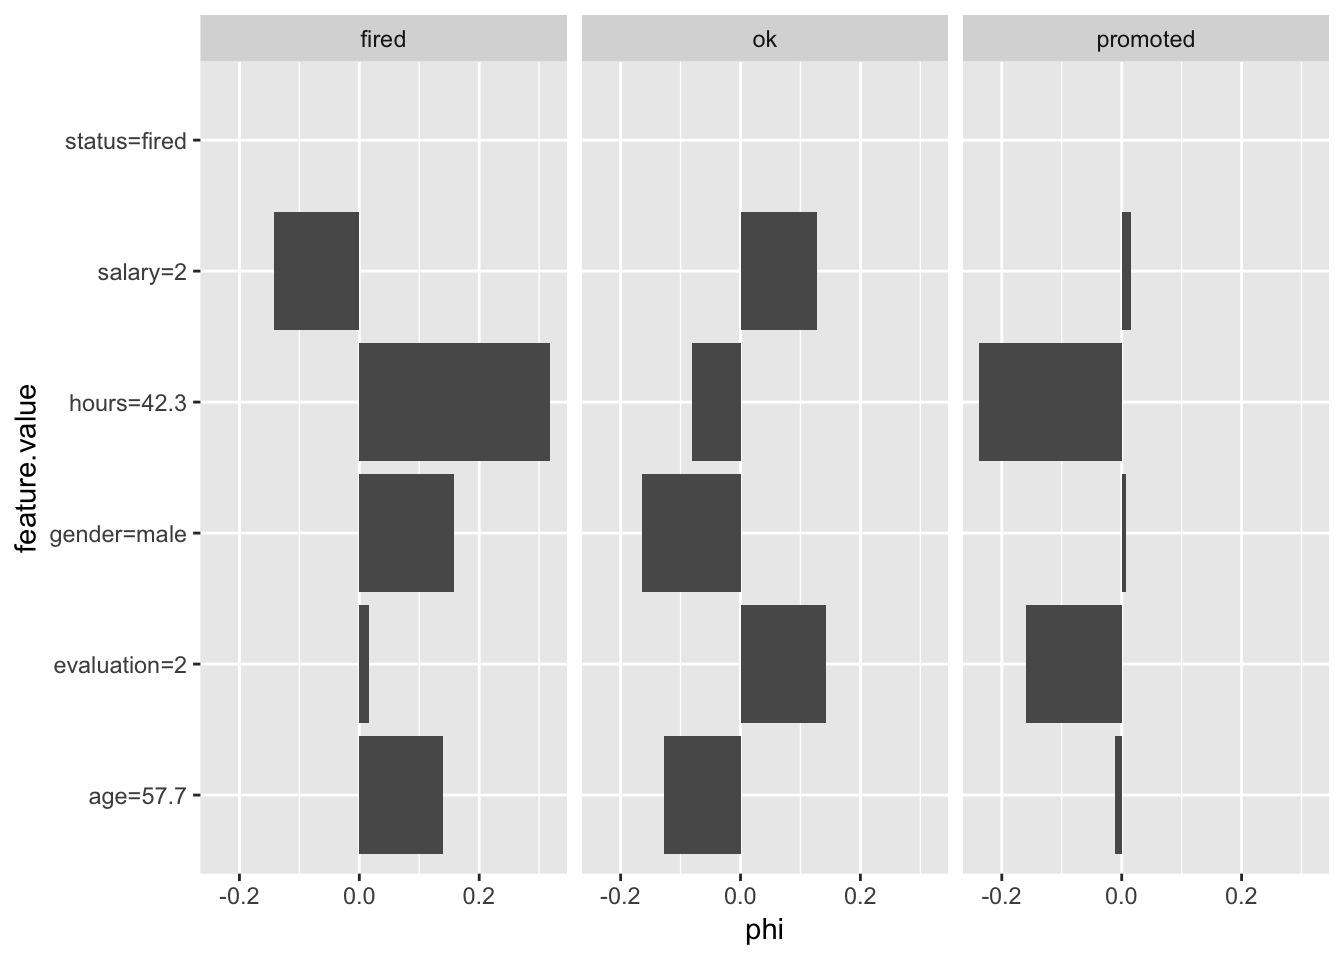
\includegraphics{PM_VEE_files/figure-latex/unnamed-chunk-18-1.pdf}

Here we use the \texttt{iml} package, see more examples in
\citep{imlPackage}.

\begin{Shaded}
\begin{Highlighting}[]
\KeywordTok{library}\NormalTok{(}\StringTok{"iml"}\NormalTok{)}
\NormalTok{explainer_rf =}\StringTok{ }\NormalTok{Predictor}\OperatorTok{$}\KeywordTok{new}\NormalTok{(model_rf, }\DataTypeTok{data =}\NormalTok{ HR, }\DataTypeTok{type=}\StringTok{"prob"}\NormalTok{)}
\end{Highlighting}
\end{Shaded}

Explanations for a new observation.

\begin{Shaded}
\begin{Highlighting}[]
\NormalTok{new_observation <-}\StringTok{ }\KeywordTok{data.frame}\NormalTok{(}\DataTypeTok{gender =} \KeywordTok{factor}\NormalTok{(}\StringTok{"male"}\NormalTok{, }\DataTypeTok{levels =} \KeywordTok{c}\NormalTok{(}\StringTok{"male"}\NormalTok{, }\StringTok{"female"}\NormalTok{)),}
                      \DataTypeTok{age =} \FloatTok{57.7}\NormalTok{,}
                      \DataTypeTok{hours =} \FloatTok{42.3}\NormalTok{,}
                      \DataTypeTok{evaluation =} \DecValTok{2}\NormalTok{,}
                      \DataTypeTok{salary =} \DecValTok{2}\NormalTok{,}
                      \DataTypeTok{status =} \KeywordTok{factor}\NormalTok{(}\StringTok{"fired"}\NormalTok{))}

\NormalTok{shapley =}\StringTok{ }\NormalTok{Shapley}\OperatorTok{$}\KeywordTok{new}\NormalTok{(explainer_rf, }\DataTypeTok{x.interest =}\NormalTok{ new_observation)}
\NormalTok{shapley}
\end{Highlighting}
\end{Shaded}

\begin{verbatim}
## Interpretation method:  Shapley 
## Predicted value: 0.768000, Average prediction: 0.375522 (diff = 0.392478) Predicted value: 0.232000, Average prediction: 0.275811 (diff = -0.043811) Predicted value: 0.000000, Average prediction: 0.348667 (diff = -0.348667)
## 
## Analysed predictor: 
## Prediction task: unknown 
## 
## 
## Analysed data:
## Sampling from data.frame with 7847 rows and 6 columns.
## 
## Head of results:
##      feature class      phi    phi.var feature.value
## 1     gender fired  0.15184 0.06525201   gender=male
## 2        age fired  0.10980 0.07939374      age=57.7
## 3      hours fired  0.23736 0.11281486    hours=42.3
## 4 evaluation fired  0.03640 0.01645164  evaluation=2
## 5     salary fired -0.17504 0.04931632      salary=2
## 6     status fired  0.00000 0.00000000  status=fired
\end{verbatim}

And the plot with Shapley attributions.

\begin{Shaded}
\begin{Highlighting}[]
\KeywordTok{plot}\NormalTok{(shapley)}
\end{Highlighting}
\end{Shaded}

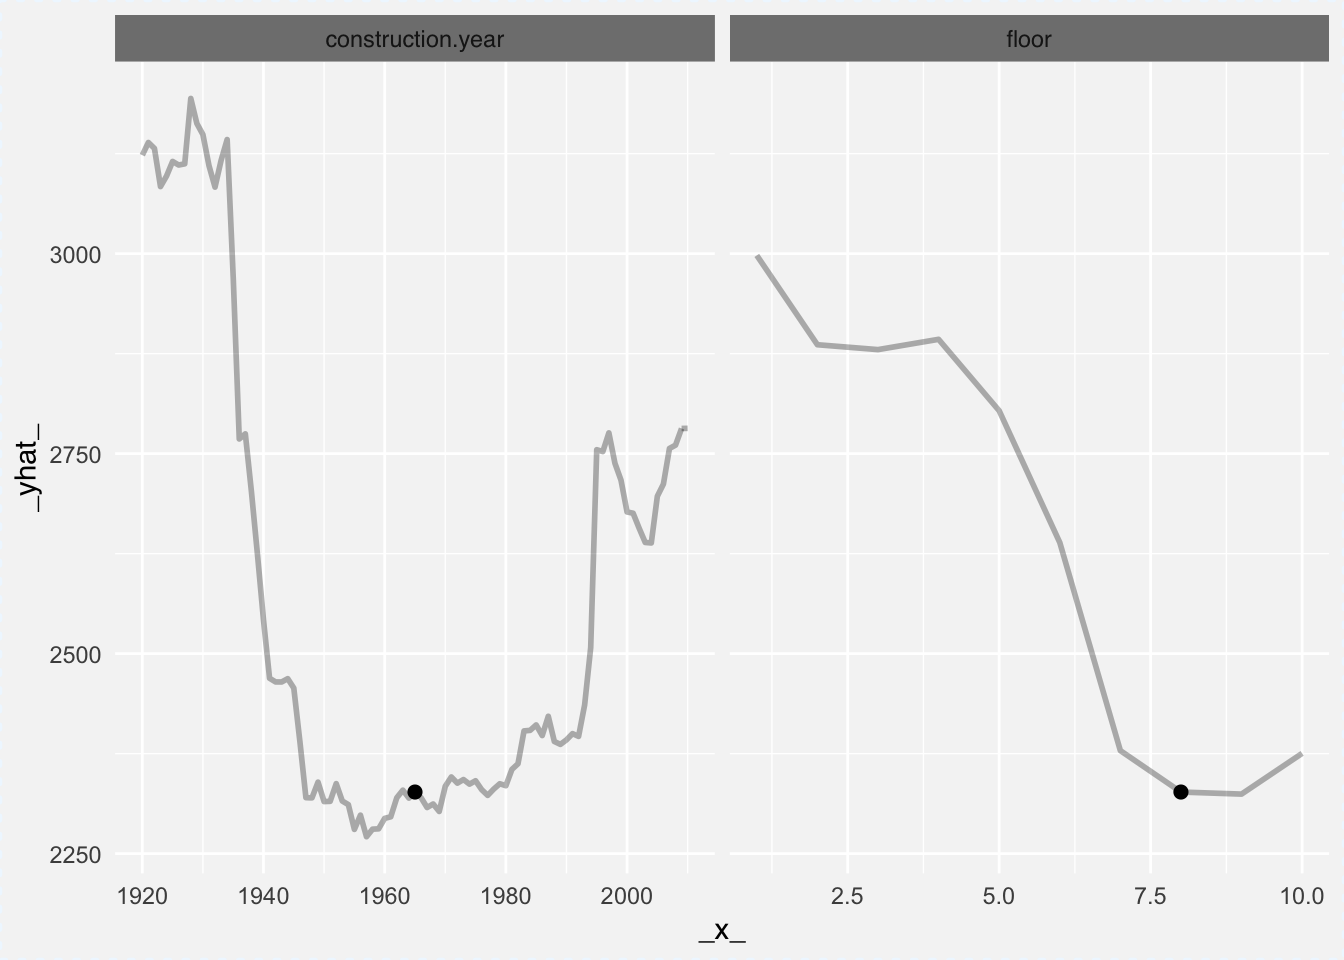
\includegraphics{PM_VEE_files/figure-latex/unnamed-chunk-21-1.pdf}

See more examples for \texttt{iml} package in the \citep{molnar} book.

\hypertarget{LIME}{%
\section{Local approximations with white-box model}\label{LIME}}

A different approach to explanations of a single observations is through
surrogate models. Models that easy to understand and are similar to
black box model around the point of interest.

Variable attribution methods, that were presented in the Section
\ref{breakDown} are not interested in the local curvature of the model.
They rather compare model prediction against average model prediction
and they use probability structure of the dataset.

The complementary approach would be to directly explore information
about model curvature around point of interest. In the section
\ref{ceterisParibus} we introduced Ceteris Paribus tool for such what-if
analysis. But the limitation of ceteris Paribus pltos is that they
explore changes along single dimension or pairs of dimensions.

In this section we describe an another approach based on local
approximations with white-box models. This approach will also
investigate local curvature of the model but indirectly, through
surrogate white-box models.

The most known method from this class if LIME (Local Interpretable
Model-Agnostic Explanations), introduced in the paper \emph{Why Should I
Trust You?: Explaining the Predictions of Any Classifier} \citep{lime}.
This methods and it's clones are now implemented in various R and python
packages, see for example \citep{R-lime}, \citep{R-live} or
\citep{R-iml}.

\hypertarget{intuition-4}{%
\subsection{Intuition}\label{intuition-4}}

\hypertarget{method-4}{%
\subsection{Method}\label{method-4}}

The LIME method, and its clones, has following properties:

\begin{itemize}
\tightlist
\item
  \emph{model-agnostic}, they do not imply any assumptions on model
  structure,
\item
  \emph{interpretable representation}, model input is transformed into a
  feature space that is easier to understand. One of applications comes
  from image data, single pixels are not easy to interpret, thus the
  LIME method decompose image into a series of super pixels, that are
  easier to interpret to humans,
\item
  \emph{local fidelity} means that the explanations shall be locally
  well fitted to the black-box model.
\end{itemize}

Therefore the objective is to find a local model \(M^L\) that
approximates the black box model \(f\) in the point \(x^*\). As a
solution the penalized loss function is used. The white-box model that
is used for explanations satisfies following condition.

\[
M^*(x^*) = \arg \min_{g \in G} L(f, g, \Pi_{x^*}) + \Omega (g) 
\] where \(G\) is a family of white box models (e.g.~linear models),
\(\Pi_{x^*}\) is neighbourhood of \(x^*\) and \(\Omega\) stands for
model complexity.

\begin{figure}

{\centering 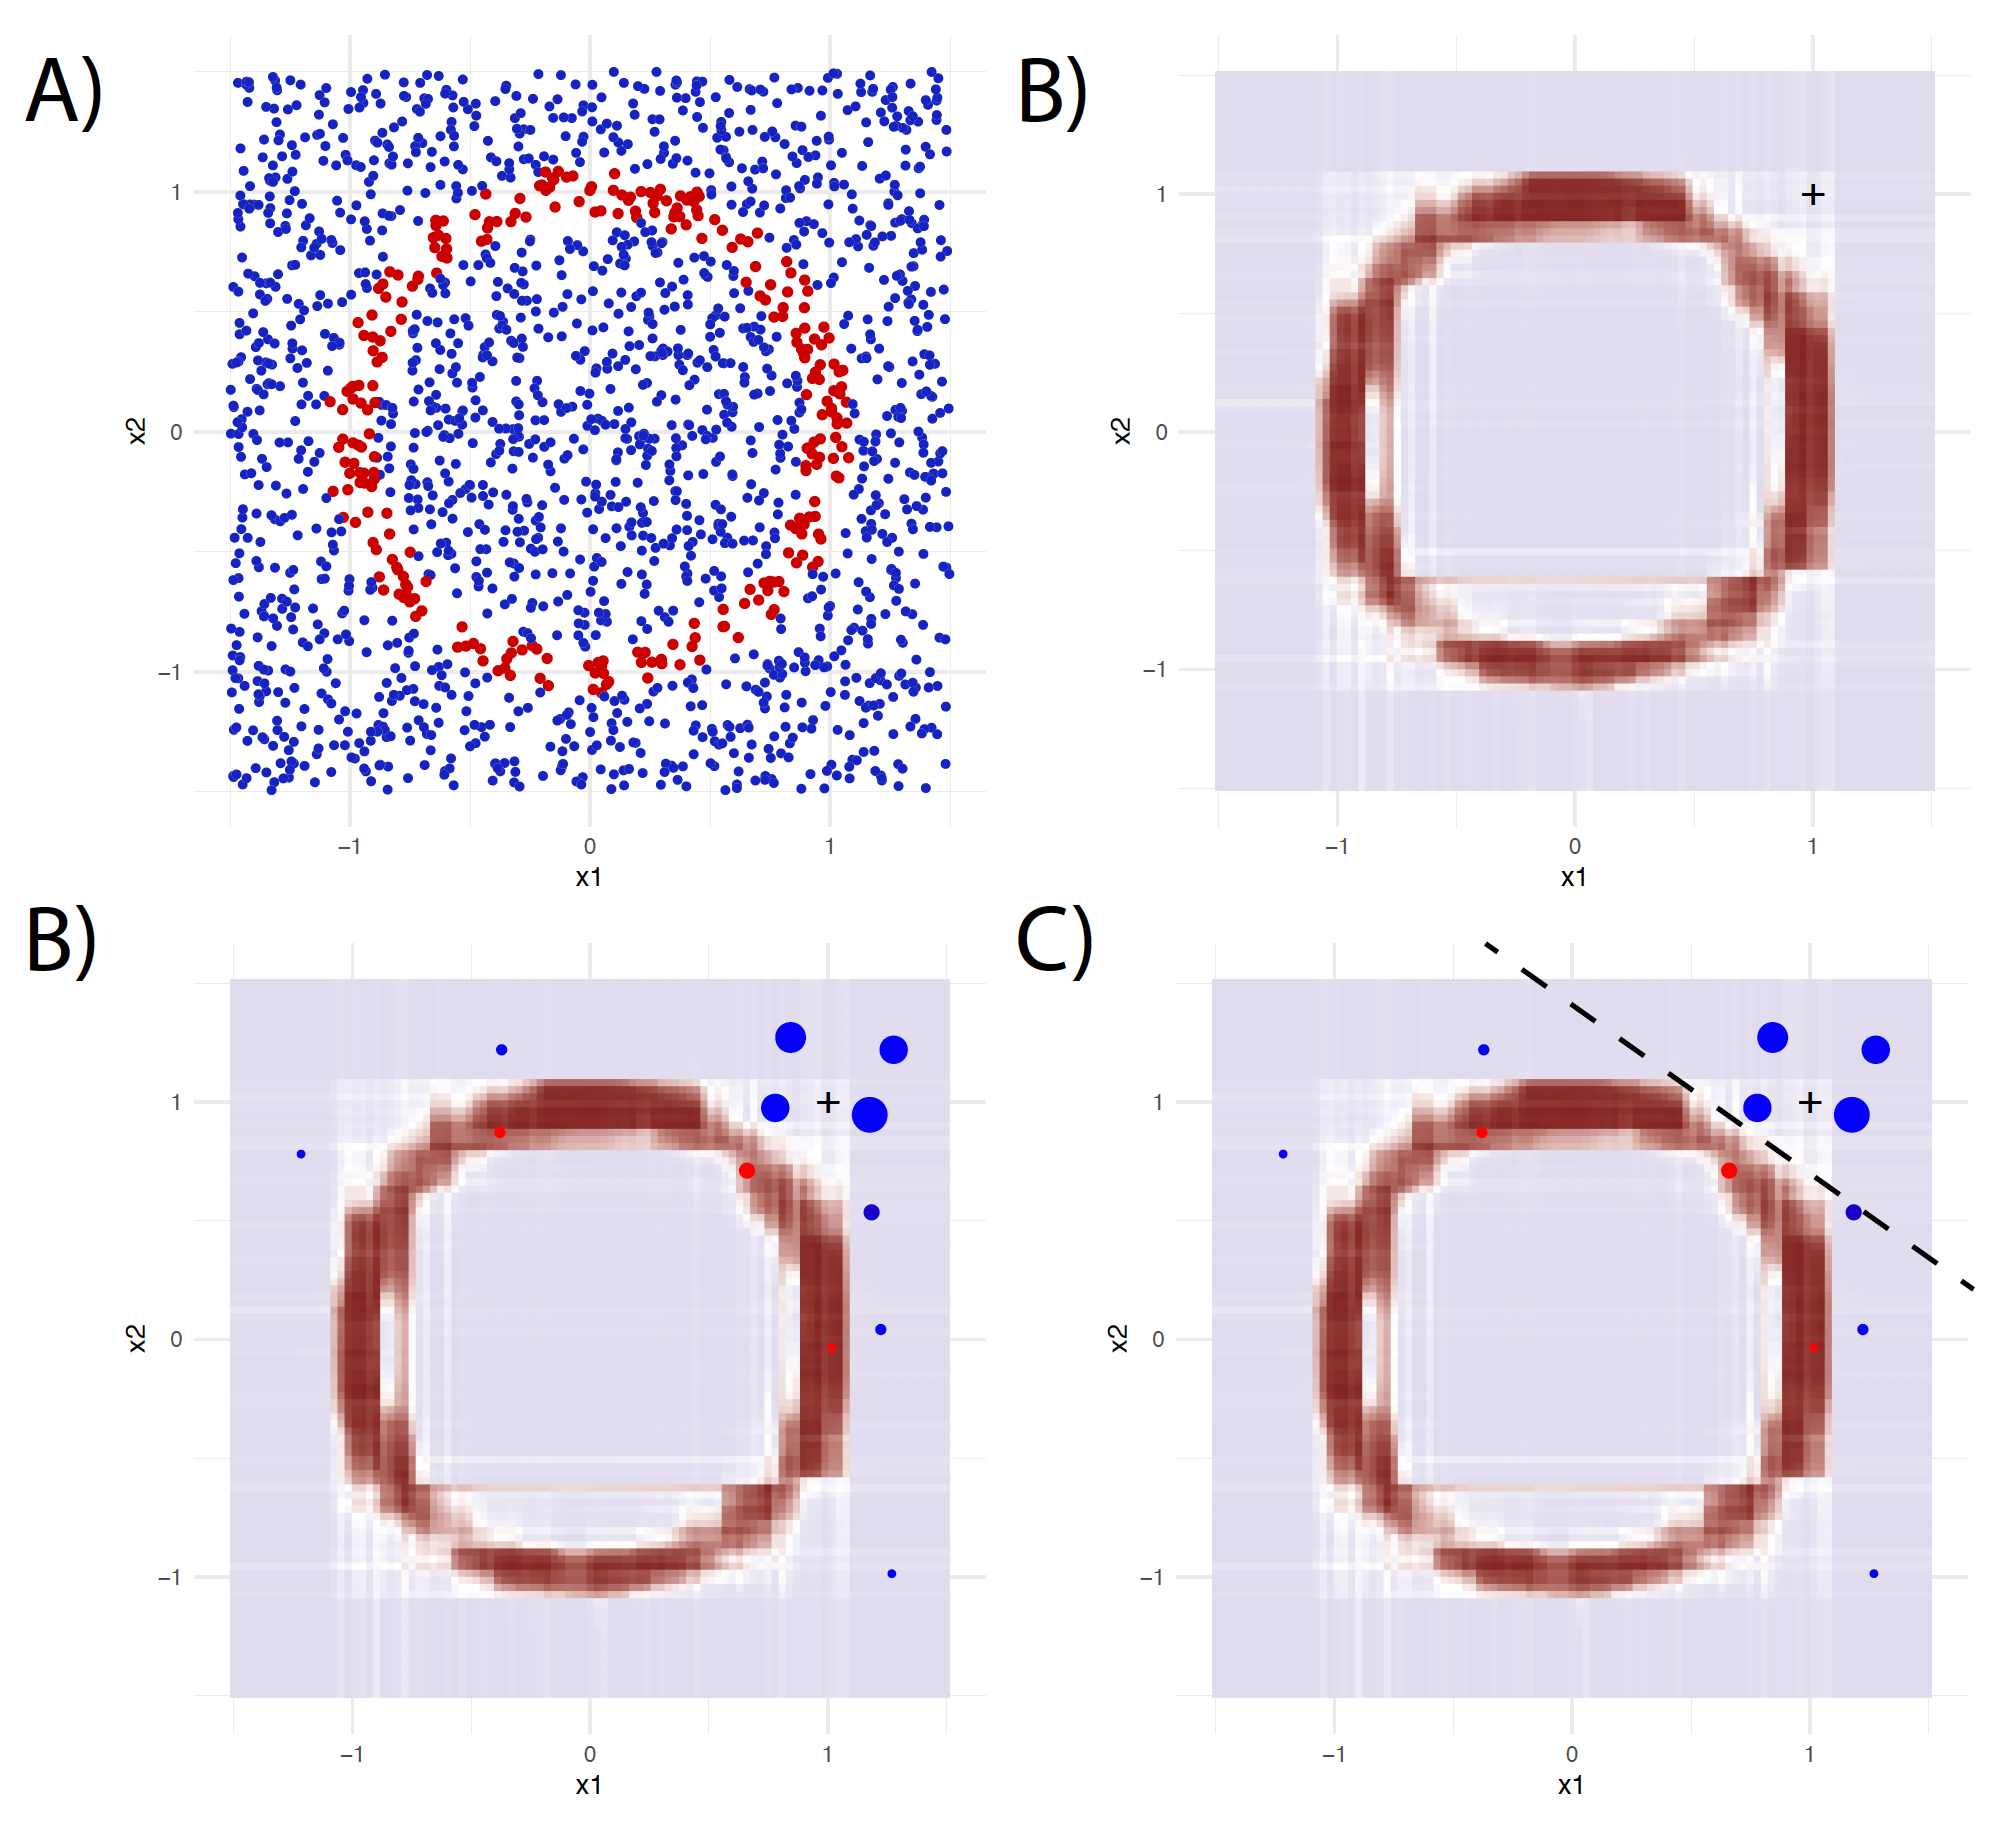
\includegraphics[width=0.7\linewidth]{figure/circle_4panels} 

}

\caption{(fig:LIME1) A schematic idea behind local model approximations. Panel A shows training data, colors correspond to classess. Panel B showhs results fom the Random Forest model, whis is where the algorithm starts. Panel C shows new data sampled around the point of interest. Their color correspond to model response. Panel D shows fitted linear model that approximated the random forest model around point of interest}\label{fig:LIME1}
\end{figure}

The algorithm is composed from three steps:

\begin{itemize}
\tightlist
\item
  Identification of interpretable data representations,
\item
  Local sampling around the point of interest,
\item
  Fitting a white box model in this neighbouhood
\end{itemize}

\textbf{Identification of interpretable data representations}

For image data, single pixel is not an interpretable feature. In this
step the input space of the model is transformed to input space that is
easier to understand for human. The image may be decomposed into parts
and represented as presence/absence of some part of an image.

\textbf{Local sampling around the point of interest}

Once the interpretable data representation is identified, then the
neighbourhood around point of interest needs to be explored.

\textbf{Fitting a white box model in this neighbouhood}

Any model that is easy to interpret may be fitted to this data, like
decision tree or rule based system. However in practice the most common
family of models are linear models.

\hypertarget{example-hire-or-fire-3}{%
\subsection{Example: Hire or Fire?}\label{example-hire-or-fire-3}}

\hypertarget{pros-and-cons-4}{%
\subsection{Pros and cons}\label{pros-and-cons-4}}

Local approximations are model agnostic, can be applied to any
predictive model. Below we summarize key strengths and weaknesses of
this approach.

\textbf{Pros}

\begin{itemize}
\tightlist
\item
  This method is highly adopted in text analysis and image analysis, in
  part thanks to the interpretable data representations.
\item
  The intuition behind the model is straightforward
\item
  Model explanations are sparse, thus only small number of features is
  used
\end{itemize}

\textbf{Cons}

\begin{itemize}
\tightlist
\item
  For continuous variables and tabular data it is not that easy to find
  interpretable representations
\item
  The black-box model approximated the data and the white box model
  approximates the black box model. We do not have control over the
  quality of local fit of the white box model, thus the surrogate model
  may be misleading.
\item
  Due to the \emph{curse of dimensionality}, for high dimensional space
  points are sparse.
\end{itemize}

\hypertarget{code-snippets-for-r-3}{%
\subsection{Code snippets for R}\label{code-snippets-for-r-3}}

In this section we present example application of \texttt{lime}
\citep{R-lime} and \texttt{live} \citep{R-live} packages. Note that this
method is also implemented in \texttt{iml} \citep{R-iml} and other
packages. These pacakages differ in some details and also results in
different explanations.

\textbf{Model preparation}

In this section we will present examples based on the \texttt{HR}
dataset. See the Section \ref{HRdataset} for more details.

\begin{Shaded}
\begin{Highlighting}[]
\KeywordTok{library}\NormalTok{(}\StringTok{"DALEX"}\NormalTok{)}
\KeywordTok{head}\NormalTok{(HR)}
\end{Highlighting}
\end{Shaded}

\begin{verbatim}
##   gender      age    hours evaluation salary   status
## 1   male 32.58267 41.88626          3      1    fired
## 2 female 41.21104 36.34339          2      5    fired
## 3   male 37.70516 36.81718          3      0    fired
## 4 female 30.06051 38.96032          3      2    fired
## 5   male 21.10283 62.15464          5      3 promoted
## 6   male 40.11812 69.53973          2      0    fired
\end{verbatim}

The problem here is to predict average price for square meter for an
apartment. Let's build a random forest model with \texttt{randomForest}
package \citep{R-randomForest}.

\begin{Shaded}
\begin{Highlighting}[]
\KeywordTok{library}\NormalTok{(}\StringTok{"randomForest"}\NormalTok{)}
\NormalTok{rf_model <-}\StringTok{ }\KeywordTok{randomForest}\NormalTok{(status }\OperatorTok{~}\StringTok{ }\NormalTok{gender }\OperatorTok{+}\StringTok{ }\NormalTok{age }\OperatorTok{+}\StringTok{ }\NormalTok{hours }\OperatorTok{+}\StringTok{ }\NormalTok{evaluation }\OperatorTok{+}\StringTok{ }\NormalTok{salary, }\DataTypeTok{data =}\NormalTok{ HR)}
\NormalTok{rf_model}
\end{Highlighting}
\end{Shaded}

\begin{verbatim}
## 
## Call:
##  randomForest(formula = status ~ gender + age + hours + evaluation +      salary, data = HR) 
##                Type of random forest: classification
##                      Number of trees: 500
## No. of variables tried at each split: 2
## 
##         OOB estimate of  error rate: 27.4%
## Confusion matrix:
##          fired   ok promoted class.error
## fired     2274  380      201   0.2035026
## ok         539 1235      447   0.4439442
## promoted   199  384     2188   0.2103934
\end{verbatim}

\begin{Shaded}
\begin{Highlighting}[]
\NormalTok{new_observation <-}\StringTok{ }\KeywordTok{data.frame}\NormalTok{(}\DataTypeTok{gender =} \KeywordTok{factor}\NormalTok{(}\StringTok{"male"}\NormalTok{, }\DataTypeTok{levels =} \KeywordTok{c}\NormalTok{(}\StringTok{"male"}\NormalTok{, }\StringTok{"female"}\NormalTok{)),}
                      \DataTypeTok{age =} \FloatTok{57.7}\NormalTok{,}
                      \DataTypeTok{hours =} \FloatTok{42.3}\NormalTok{,}
                      \DataTypeTok{evaluation =} \DecValTok{2}\NormalTok{,}
                      \DataTypeTok{salary =} \DecValTok{2}\NormalTok{)}

\KeywordTok{predict}\NormalTok{(rf_model, new_observation, }\DataTypeTok{type =} \StringTok{"prob"}\NormalTok{)}
\end{Highlighting}
\end{Shaded}

\begin{verbatim}
##   fired    ok promoted
## 1 0.806 0.192    0.002
## attr(,"class")
## [1] "matrix" "votes"
\end{verbatim}

\hypertarget{the-lime-pacakge}{%
\subsubsection{\texorpdfstring{\textbf{The lime
pacakge}}{The lime pacakge}}\label{the-lime-pacakge}}

\begin{Shaded}
\begin{Highlighting}[]
\KeywordTok{library}\NormalTok{(}\StringTok{"lime"}\NormalTok{)}
\NormalTok{model_type.randomForest <-}\StringTok{ }\ControlFlowTok{function}\NormalTok{(x, ...) }\StringTok{"classification"}
\NormalTok{lime_rf <-}\StringTok{ }\KeywordTok{lime}\NormalTok{(HR[,}\DecValTok{1}\OperatorTok{:}\DecValTok{5}\NormalTok{], rf_model)}
\NormalTok{explanations <-}\StringTok{ }\NormalTok{lime}\OperatorTok{::}\KeywordTok{explain}\NormalTok{(new_observation[,}\DecValTok{1}\OperatorTok{:}\DecValTok{5}\NormalTok{], lime_rf, }\DataTypeTok{n_labels =} \DecValTok{3}\NormalTok{, }\DataTypeTok{n_features =} \DecValTok{3}\NormalTok{)}
\NormalTok{explanations}
\end{Highlighting}
\end{Shaded}

\begin{verbatim}
##       model_type case    label label_prob  model_r2 model_intercept
## 1 classification    1    fired      0.806 0.1300379       0.2535829
## 2 classification    1    fired      0.806 0.1300379       0.2535829
## 3 classification    1    fired      0.806 0.1300379       0.2535829
## 4 classification    1       ok      0.192 0.1251273       0.1892168
## 5 classification    1       ok      0.192 0.1251273       0.1892168
## 6 classification    1       ok      0.192 0.1251273       0.1892168
## 7 classification    1 promoted      0.002 0.2917896       0.5234322
## 8 classification    1 promoted      0.002 0.2917896       0.5234322
## 9 classification    1 promoted      0.002 0.2917896       0.5234322
##   model_prediction    feature feature_value feature_weight
## 1       0.63245342     gender           2.0    0.005909490
## 2       0.63245342      hours          42.3    0.255709364
## 3       0.63245342 evaluation           2.0    0.117251637
## 4       0.45914034        age          57.7   -0.001159746
## 5       0.45914034 evaluation           2.0    0.199215613
## 6       0.45914034     salary           2.0    0.071867712
## 7       0.01471303        age          57.7    0.011368221
## 8       0.01471303 evaluation           2.0   -0.317045218
## 9       0.01471303      hours          42.3   -0.203042163
##           feature_desc                      data          prediction
## 1        gender = male 2.0, 57.7, 42.3, 2.0, 2.0 0.806, 0.192, 0.002
## 2 37.6 < hours <= 46.3 2.0, 57.7, 42.3, 2.0, 2.0 0.806, 0.192, 0.002
## 3      evaluation <= 3 2.0, 57.7, 42.3, 2.0, 2.0 0.806, 0.192, 0.002
## 4           50.0 < age 2.0, 57.7, 42.3, 2.0, 2.0 0.806, 0.192, 0.002
## 5      evaluation <= 3 2.0, 57.7, 42.3, 2.0, 2.0 0.806, 0.192, 0.002
## 6      1 < salary <= 2 2.0, 57.7, 42.3, 2.0, 2.0 0.806, 0.192, 0.002
## 7           50.0 < age 2.0, 57.7, 42.3, 2.0, 2.0 0.806, 0.192, 0.002
## 8      evaluation <= 3 2.0, 57.7, 42.3, 2.0, 2.0 0.806, 0.192, 0.002
## 9 37.6 < hours <= 46.3 2.0, 57.7, 42.3, 2.0, 2.0 0.806, 0.192, 0.002
\end{verbatim}

\begin{Shaded}
\begin{Highlighting}[]
\KeywordTok{plot_features}\NormalTok{(explanations)}
\end{Highlighting}
\end{Shaded}

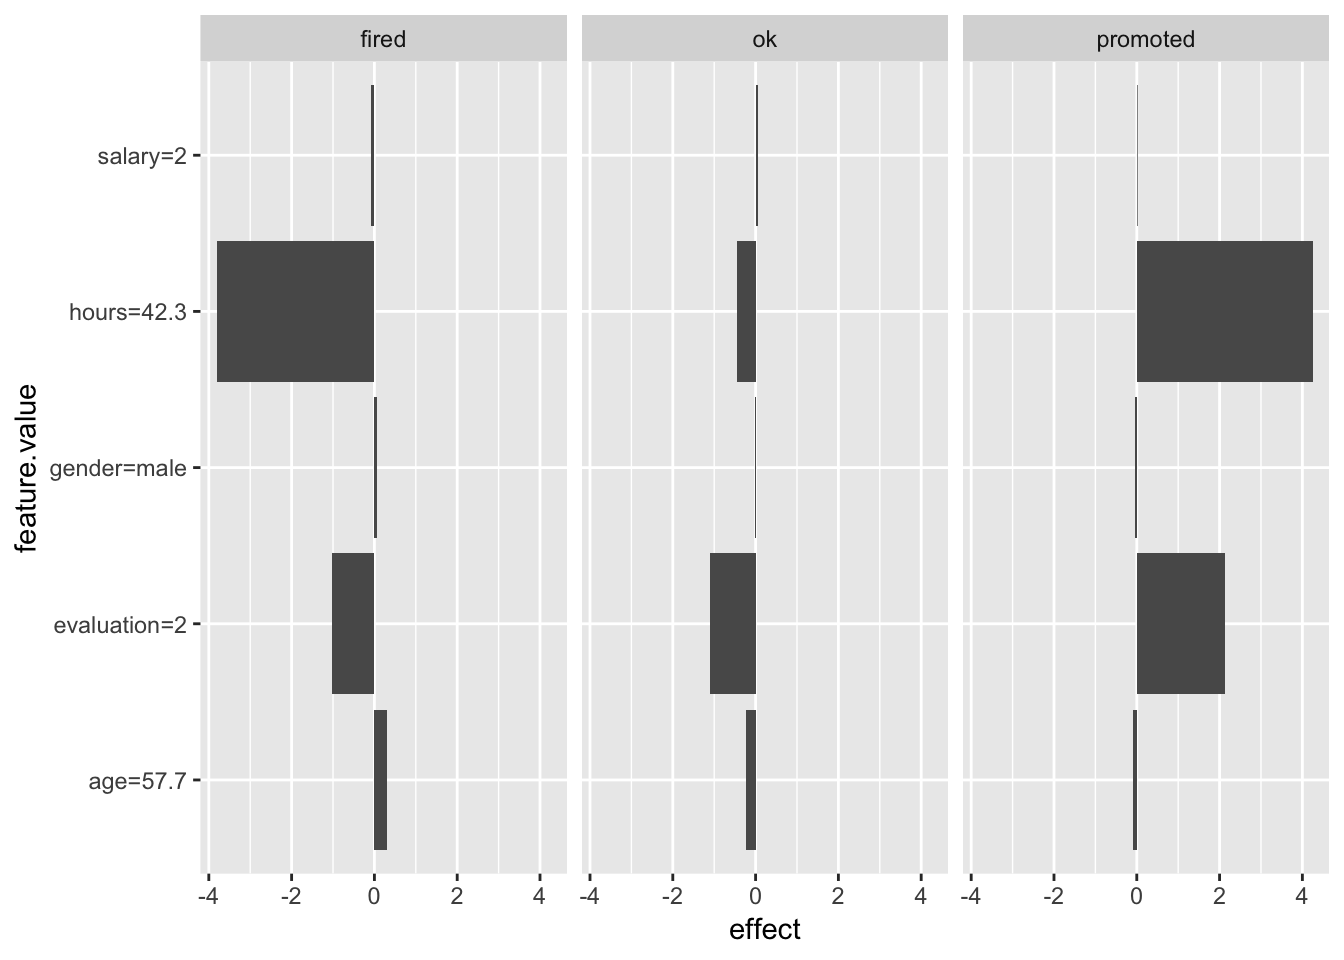
\includegraphics{PM_VEE_files/figure-latex/unnamed-chunk-26-1.pdf}

\hypertarget{the-live-package}{%
\subsubsection{\texorpdfstring{\textbf{The live
package}}{The live package}}\label{the-live-package}}

\begin{Shaded}
\begin{Highlighting}[]
\KeywordTok{library}\NormalTok{(}\StringTok{"live"}\NormalTok{)}

\NormalTok{new_observation}\OperatorTok{$}\NormalTok{status <-}\StringTok{ "fired"}
\NormalTok{explainer_rf_fired <-}\StringTok{ }\KeywordTok{explain}\NormalTok{(rf_model,}
                 \DataTypeTok{data =}\NormalTok{ HR,}
                 \DataTypeTok{y =}\NormalTok{ HR}\OperatorTok{$}\NormalTok{status }\OperatorTok{==}\StringTok{ "fired"}\NormalTok{,}
                 \DataTypeTok{predict_function =} \ControlFlowTok{function}\NormalTok{(m,x) }\KeywordTok{predict}\NormalTok{(m,x, }\DataTypeTok{type =} \StringTok{"prob"}\NormalTok{)[,}\DecValTok{1}\NormalTok{],}
                 \DataTypeTok{label =} \StringTok{"fired"}\NormalTok{)}

\NormalTok{local_model <-}\StringTok{ }\KeywordTok{local_approximation}\NormalTok{(explainer_rf_fired, new_observation, }
                    \DataTypeTok{target_variable_name =} \StringTok{"status"}\NormalTok{, }\DataTypeTok{n_new_obs =} \DecValTok{500}\NormalTok{)}

\NormalTok{local_model}
\end{Highlighting}
\end{Shaded}

\begin{verbatim}
## Dataset: 
##  Observations:  500 
##  Variables:  6 
##  Response variable:  status 
## Explanation model: 
##  Name:  regr.lm 
##  Variable selection wasn't performed 
##  Weights present in the explanation model 
##  R-squared: 0.7339
\end{verbatim}

\begin{Shaded}
\begin{Highlighting}[]
\KeywordTok{plot}\NormalTok{(local_model)}
\end{Highlighting}
\end{Shaded}

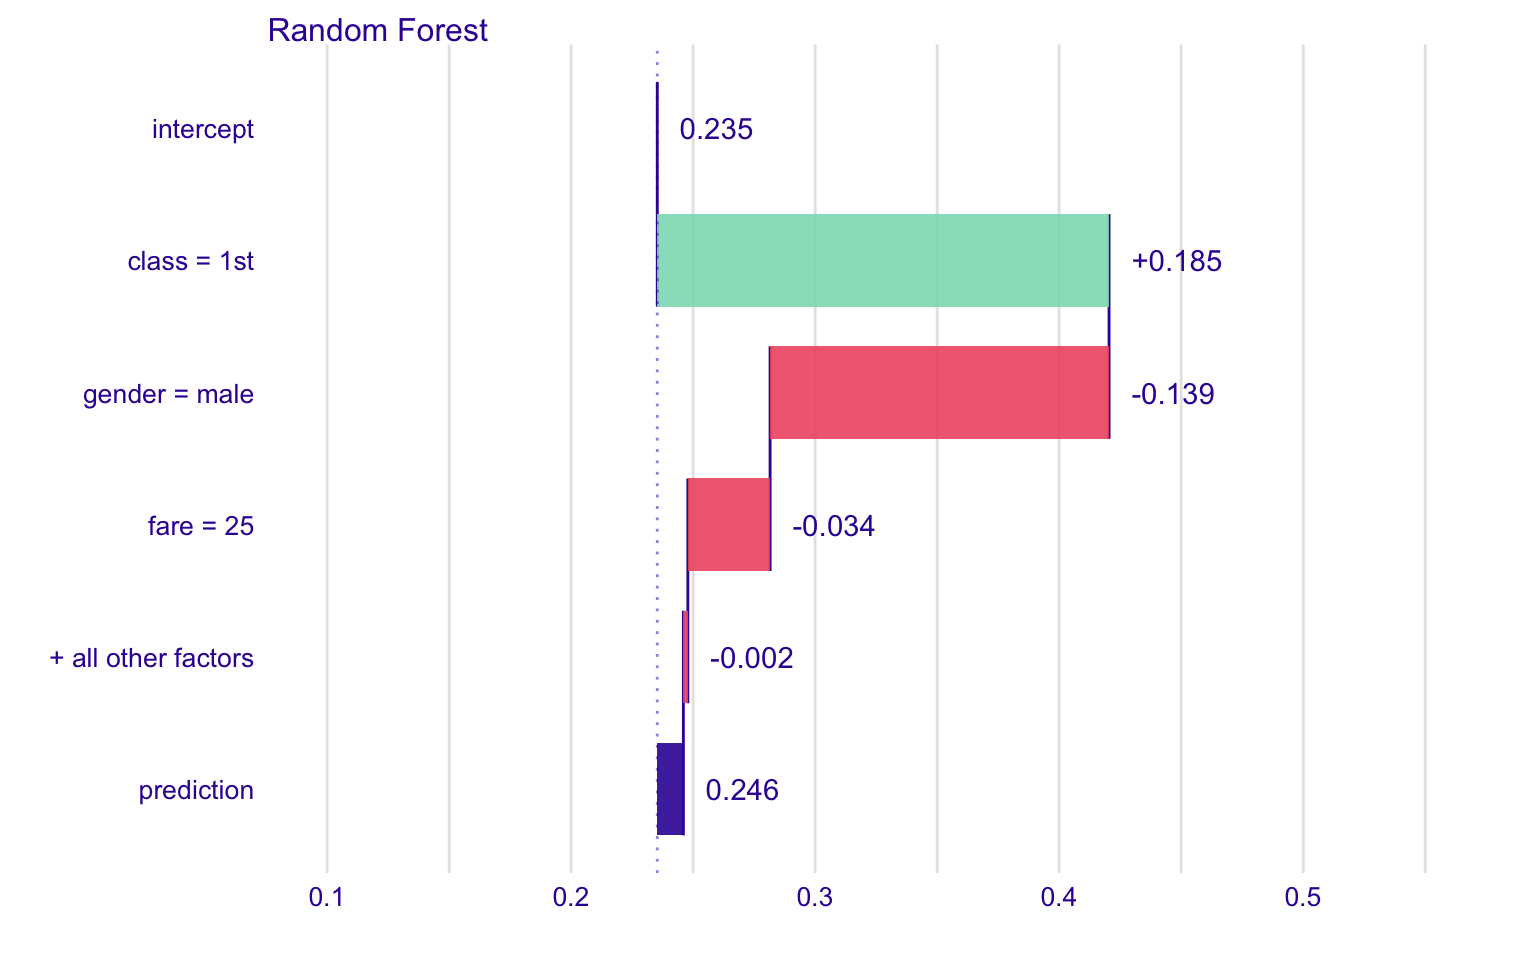
\includegraphics{PM_VEE_files/figure-latex/unnamed-chunk-27-1.pdf}

\begin{Shaded}
\begin{Highlighting}[]
\KeywordTok{plot}\NormalTok{(local_model, }\DataTypeTok{type =} \StringTok{"forest"}\NormalTok{)}
\end{Highlighting}
\end{Shaded}

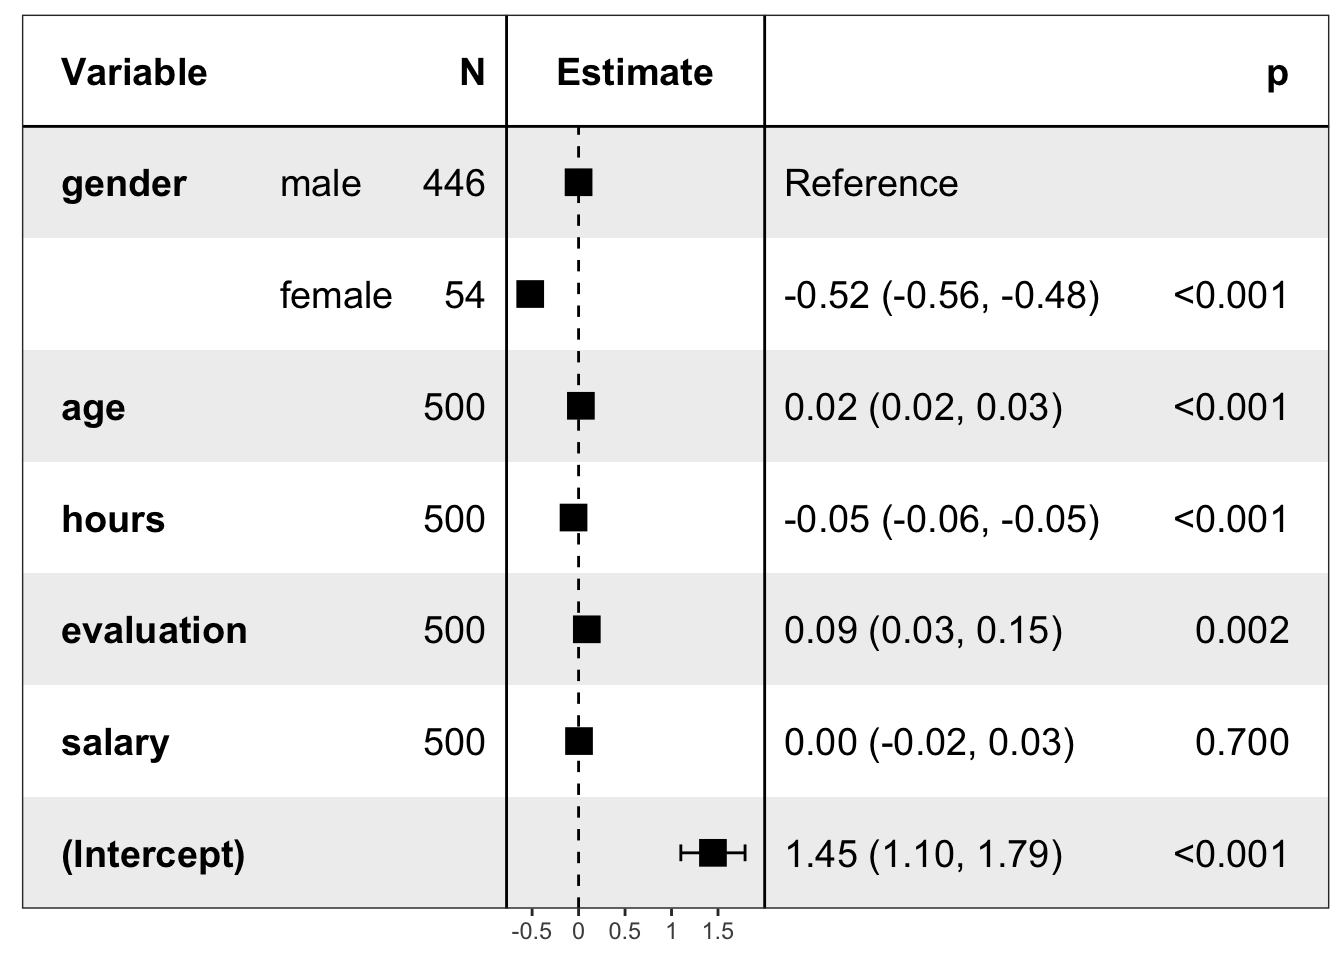
\includegraphics{PM_VEE_files/figure-latex/unnamed-chunk-27-2.pdf}

\hypertarget{the-iml-package}{%
\subsubsection{\texorpdfstring{\textbf{The iml
package}}{The iml package}}\label{the-iml-package}}

\begin{Shaded}
\begin{Highlighting}[]
\KeywordTok{library}\NormalTok{(}\StringTok{"iml"}\NormalTok{)}

\NormalTok{explainer_rf =}\StringTok{ }\NormalTok{Predictor}\OperatorTok{$}\KeywordTok{new}\NormalTok{(rf_model, }\DataTypeTok{data =}\NormalTok{ HR[,}\DecValTok{1}\OperatorTok{:}\DecValTok{5}\NormalTok{])}
\NormalTok{white_box =}\StringTok{ }\NormalTok{LocalModel}\OperatorTok{$}\KeywordTok{new}\NormalTok{(explainer_rf, }\DataTypeTok{x.interest =}\NormalTok{ new_observation[,}\DecValTok{1}\OperatorTok{:}\DecValTok{5}\NormalTok{], }\DataTypeTok{k =} \DecValTok{5}\NormalTok{)}
\NormalTok{white_box}
\end{Highlighting}
\end{Shaded}

\begin{verbatim}
## Interpretation method:  LocalModel 
## 
## 
## Analysed predictor: 
## Prediction task: unknown 
## 
## 
## Analysed data:
## Sampling from data.frame with 7847 rows and 5 columns.
## 
## Head of results:
##           beta x.recoded      effect x.original     feature feature.value
## 1  0.070451023       1.0  0.07045102       male gender=male   gender=male
## 2  0.005839379      57.7  0.33693215       57.7         age      age=57.7
## 3 -0.090103309      42.3 -3.81136995       42.3       hours    hours=42.3
## 4 -0.508252954       2.0 -1.01650591          2  evaluation  evaluation=2
## 5 -0.032191570       2.0 -0.06438314          2      salary      salary=2
## 6 -0.018323731       1.0 -0.01832373       male gender=male   gender=male
##   .class
## 1  fired
## 2  fired
## 3  fired
## 4  fired
## 5  fired
## 6     ok
\end{verbatim}

\begin{Shaded}
\begin{Highlighting}[]
\KeywordTok{plot}\NormalTok{(white_box)}
\end{Highlighting}
\end{Shaded}

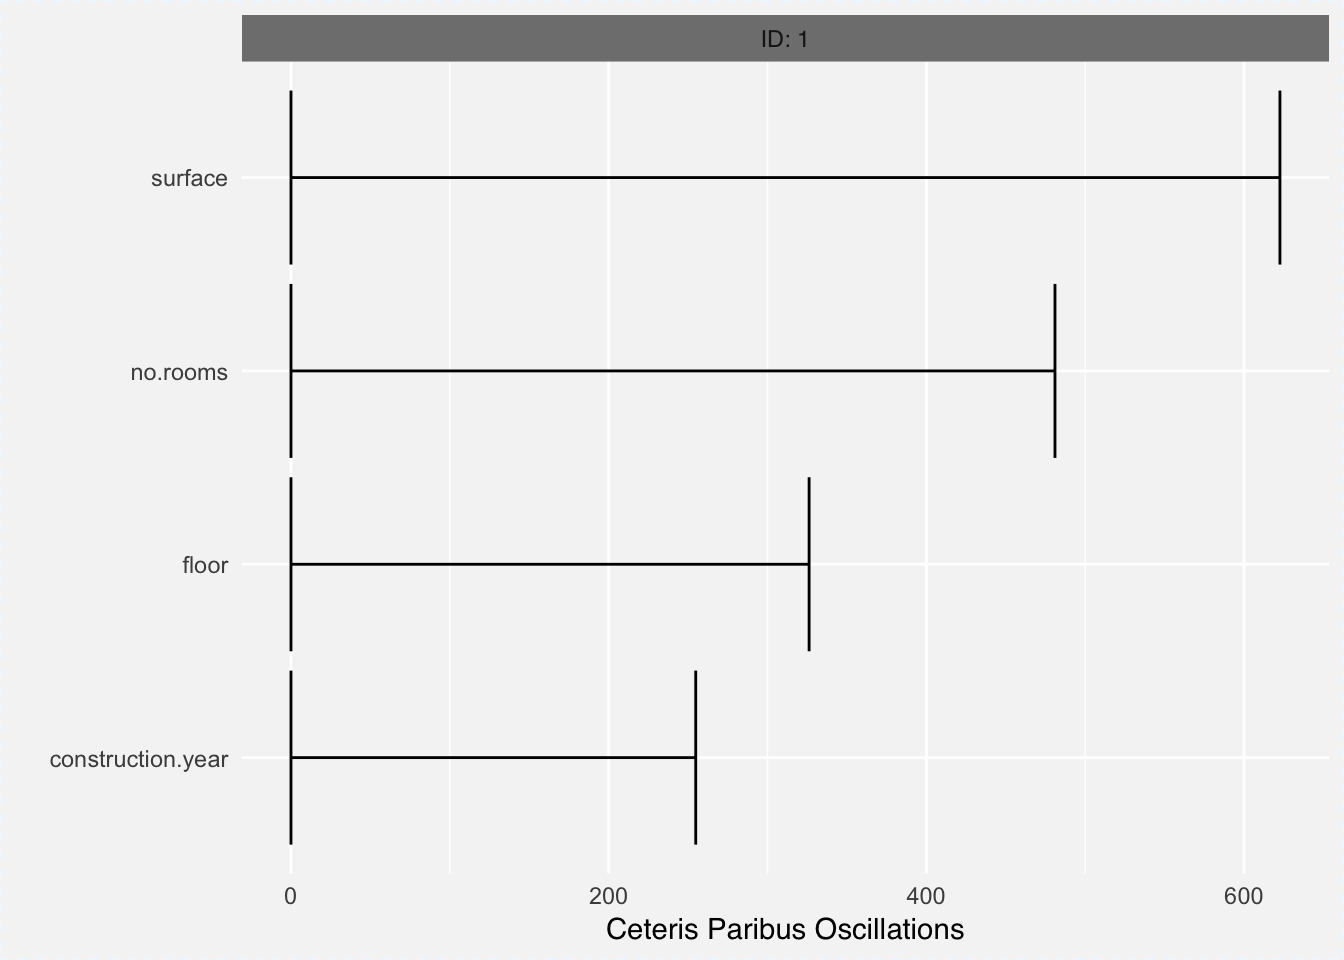
\includegraphics{PM_VEE_files/figure-latex/unnamed-chunk-28-1.pdf}

\hypertarget{ceterisParibus}{%
\section{What-If analysis with the Ceteris Paribus
Principle}\label{ceterisParibus}}

In this section we introduce tools based on Ceteris Paribus principle.
The main goal for these tools is to help understand how changes in model
input affect changes in model output.

Presented explainers are linked with the second law introduced in
Section \ref{three-single-laws}, i.e.~law for prediction's speculations.
This is why these explainers are also known as \emph{What-If model
analysis} or \emph{Individual Conditional EXpectations} \citep{ICEbox}.
It turns out that it is easier to understand how blacx-box model is
working if we can play with it by changing variable by variable.

\hypertarget{introduction-1}{%
\subsection{Introduction}\label{introduction-1}}

\emph{Ceteris paribus} is a Latin phrase meaning ``other things held
constant'' or ``all else unchanged''. Using this principle we examine
input variable per variable separatly, asumming that effects of all
other variables are unchanged. See Figure
\ref{fig:modelResponseCurveLine}

\begin{figure}

{\centering 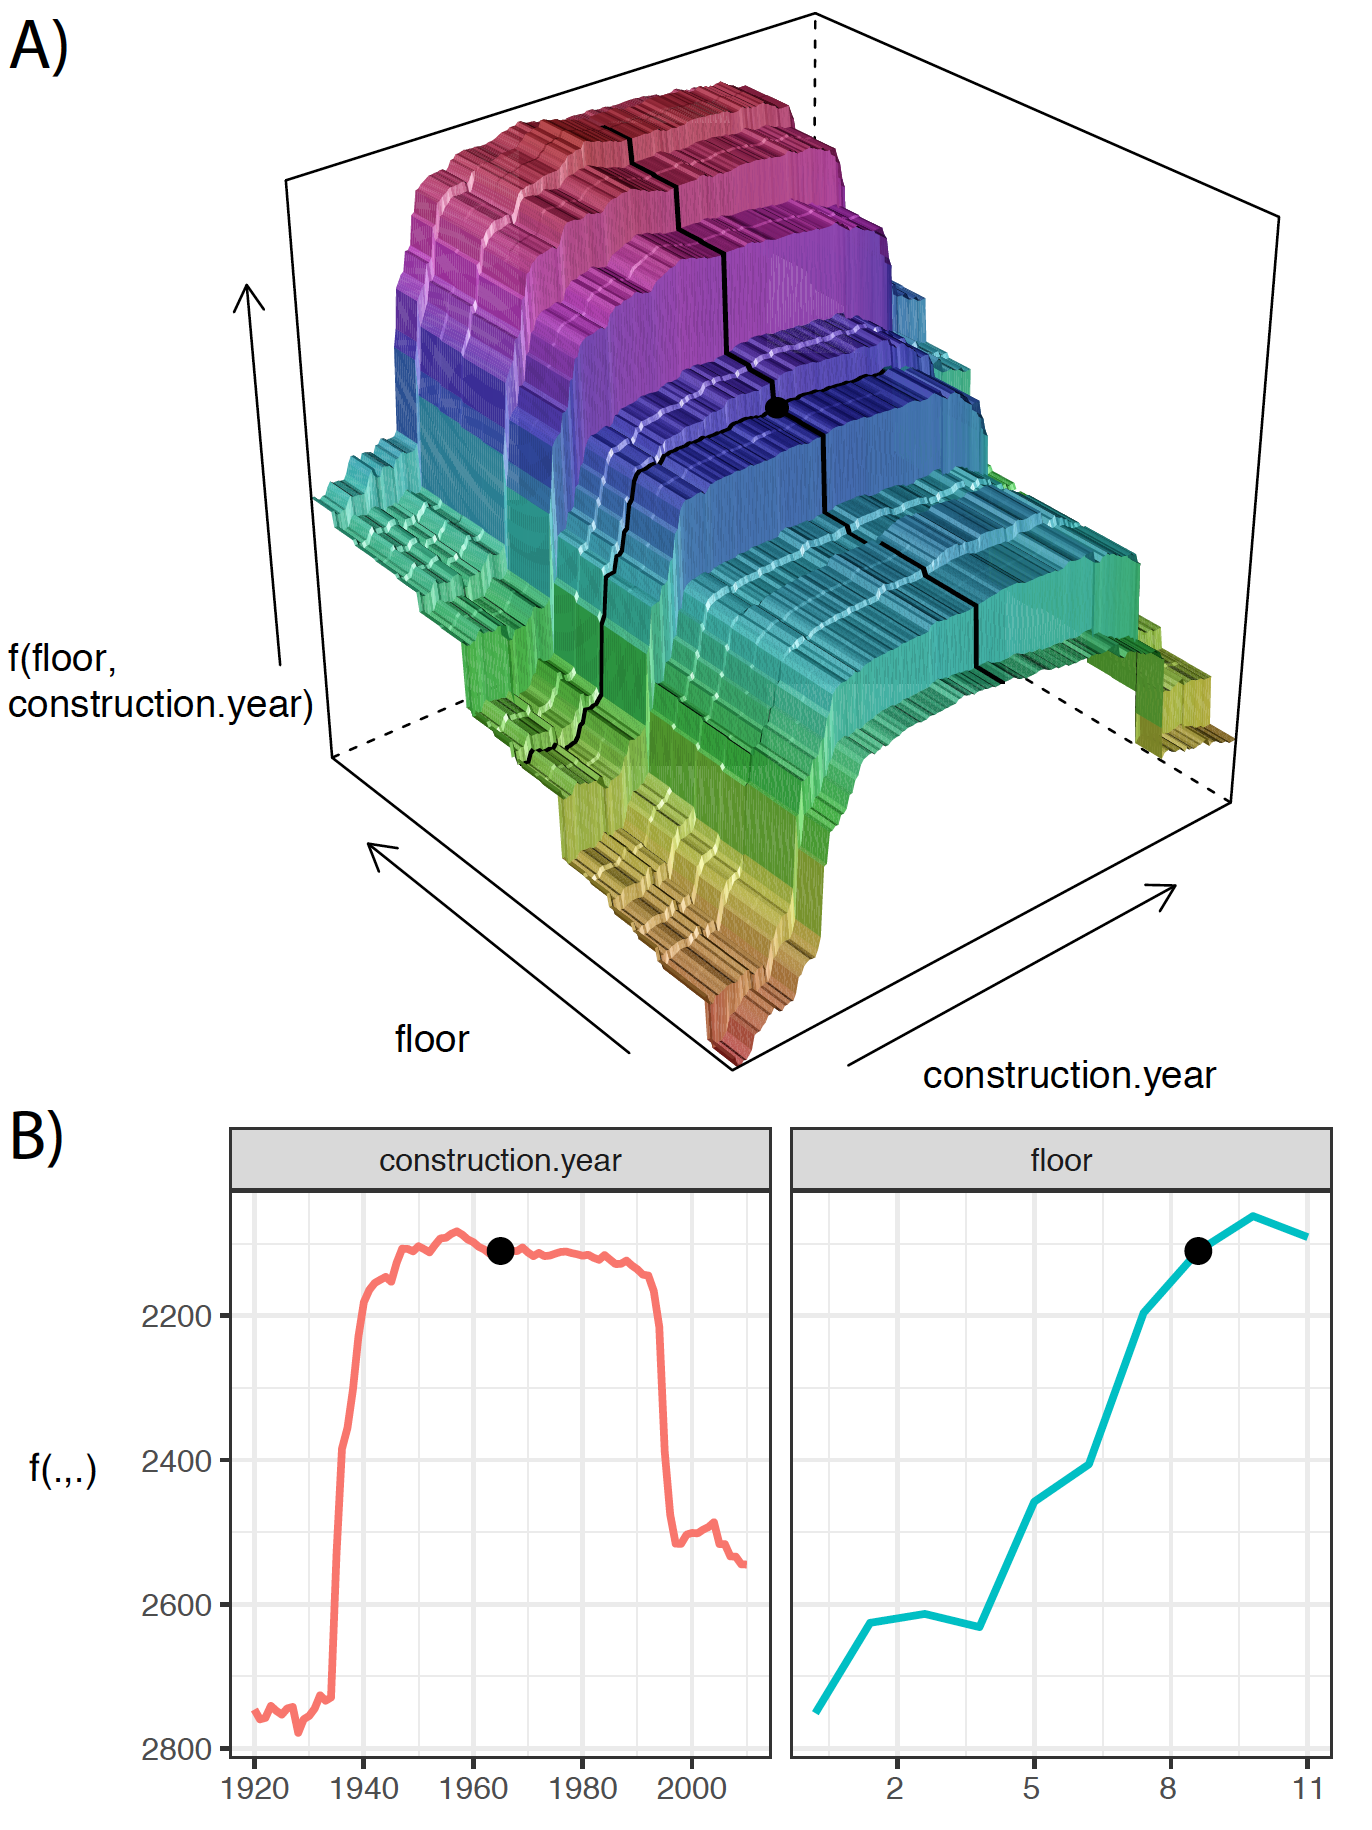
\includegraphics[width=0.7\linewidth]{figure/model_response_line} 

}

\caption{(fig:modelResponseCurveLine) A) Model response surface. Ceteris Paribus profiles marked with black curves helps to understand the curvature of the model response by updating only a single variable. B) CP profiles are individual conditional model responses}\label{fig:modelResponseCurveLine}
\end{figure}

Similar to the LIME method introduced in the section \ref{LIME}, Ceteris
Paribus profiles examine curvature of a model response function. The
difference between these two methods that LIME approximates the model
curvature with a simpler white-box model that is easier to present.
Usually the LIME model is sparse, thus our attention may be limited to
smaller number of dimensions. In contrary, the CP plots show conditional
model response for every variable. In the last subsection we discuss
pros and cons of this approach.

\hypertarget{intuition-5}{%
\subsection{Intuition}\label{intuition-5}}

\hypertarget{method-5}{%
\subsection{Method}\label{method-5}}

\hypertarget{ceterisParibus1d}{%
\subsubsection{1D profiles}\label{ceterisParibus1d}}

Let \(f_{M}(x): \mathcal R^{d} \rightarrow \mathcal R\) denote a
predictive model, i.e.~function that takes \(d\) dimensional vector and
calculate numerical score. Symbol \(x \in \mathcal R^d\) refers to a
point in the feature space. We use subscript \(x_i\) to refer to a
different data points and superscript \(x^j\) to refer to specific
dimensions. Additionally, let \(x^{-j}\) denote all coordinates except
\(j\)-th and let \(x|^j=z\) denote a data point \(x^*\) with all
coordinates equal to \(x\) except coordinate \(j\) equal to value \(z\).
I.e. \(\forall_{i \neq {j}} x^i = x^{*,i}\) and \(x^j = z\). In other
words \(x|^j=z\) denote a \(x\) with \(j\)th coordinate changed to
\(z\).

Now we can define uni-dimensional Ceteris Paribus Profile for model
\(f\), variable \(j\) and point \(x\) as

\[
CP^{f, j, x}(z) := f(x|^j = z).
\] I.e. CP profile is a model response obtained for observations created
based on \(x\) with coordinate \(j\) changed and all other coordinates
kept unchanged.

A natural way to visualise CP profiles is to use a profile plot as in
Figure \ref{fig:HRCPFiredHours}.

Figure \ref{fig:HRCPFiredHours} shows an example of Ceteris Paribus
profile. The black dot stands for prediction for a single observation.
Grey line show how the model response would change if in this single
observation coordinate \texttt{hours} will be changed to selected value.
One thing that we can read is that the model response is not smooth and
there is some variability along the profile. Second thing is that for
this particular observation the model response would drop significantly
if the variable \texttt{hours} will be higher than 45.

\begin{figure}

{\centering 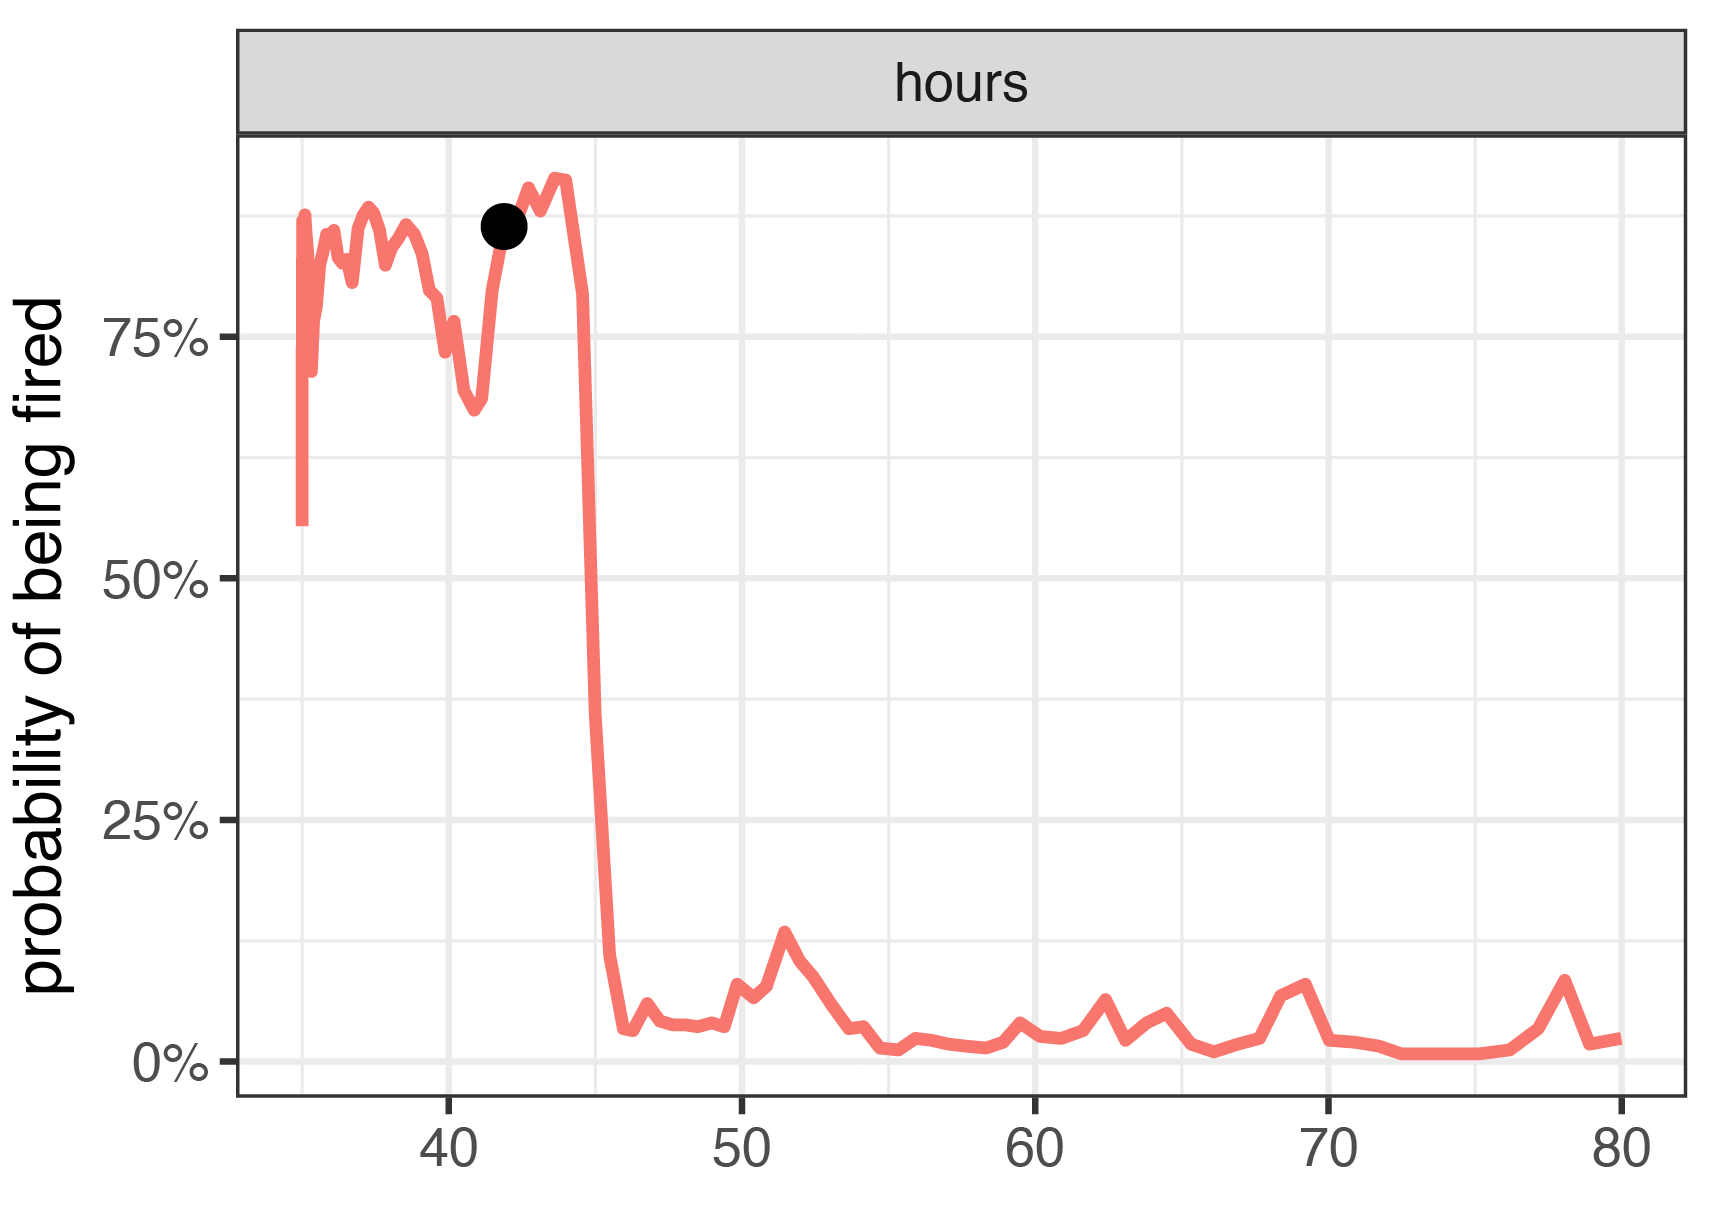
\includegraphics[width=0.5\linewidth]{figure/HR_cp_fired_hours} 

}

\caption{(fig:HRCPHiredHours) Ceteris Paribus profile for Random Forest model that assess the probability of being fired in call center as a function of average number of working hours}\label{fig:HRCPFiredHours}
\end{figure}

Since in the example dataset we are struggling with model for three
classes, one can plot CP profiles for each class in the same panel. See
an example in the Figure \ref{fig:HRCPAllHours}.

\begin{figure}

{\centering 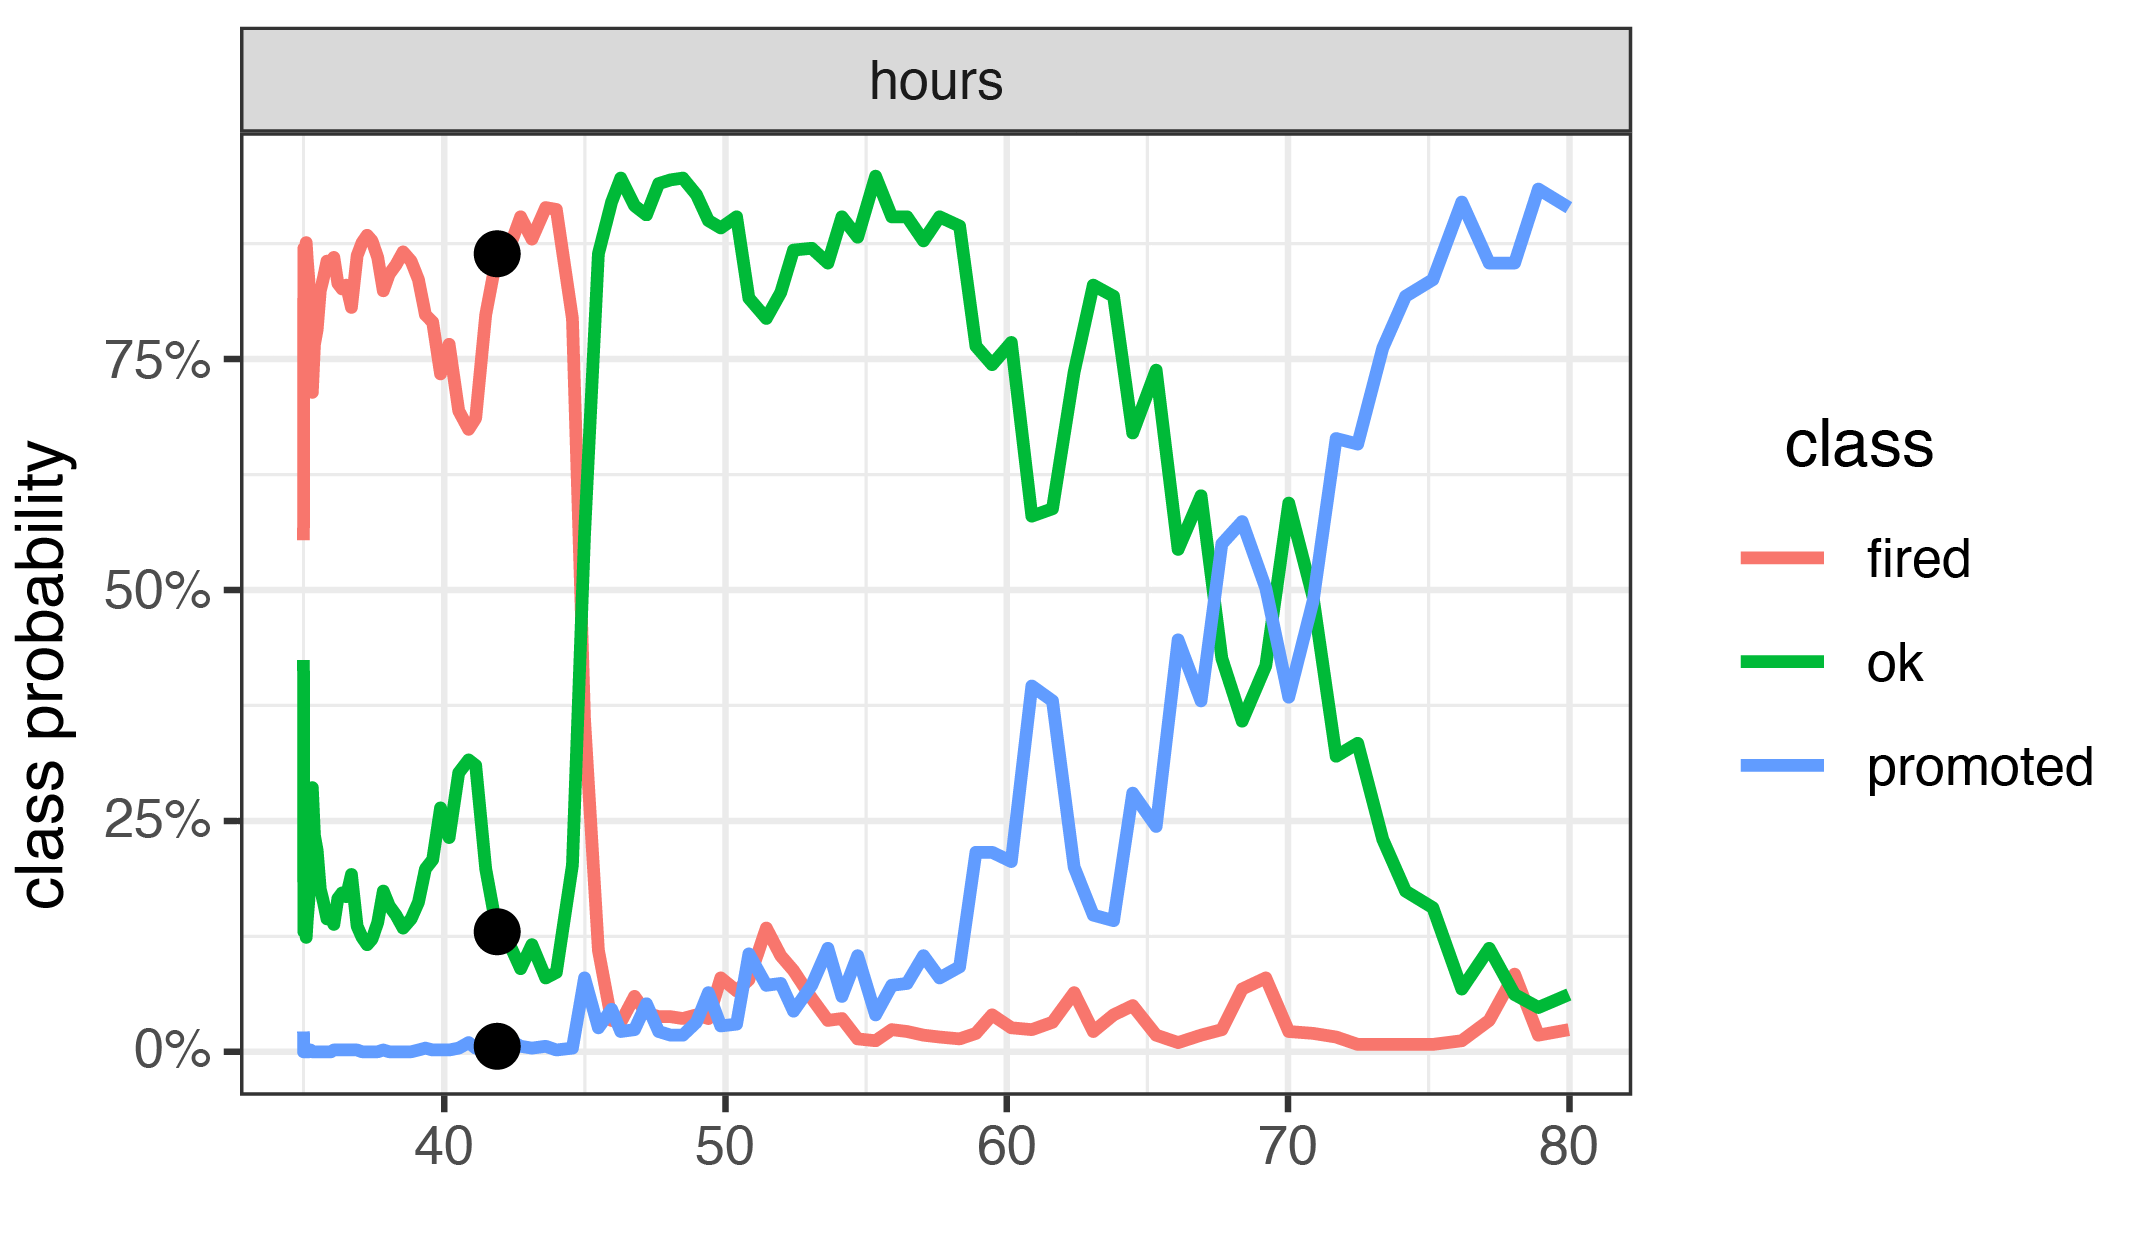
\includegraphics[width=0.6\linewidth]{figure/HR_cp_all_hours} 

}

\caption{(fig:HRCPAllHours) Ceteris Paribus profiles for three classess predicted by the Random Forest model as a function of average number of working hours}\label{fig:HRCPAllHours}
\end{figure}

Usually model input consist many variables, then it is beneficial to
show more variables at the same time. The easiest way to do so is to
plot consecutive variables on separate panels. See an example in Figure
\ref{fig:HRCPFiredAll}.

\begin{figure}

{\centering 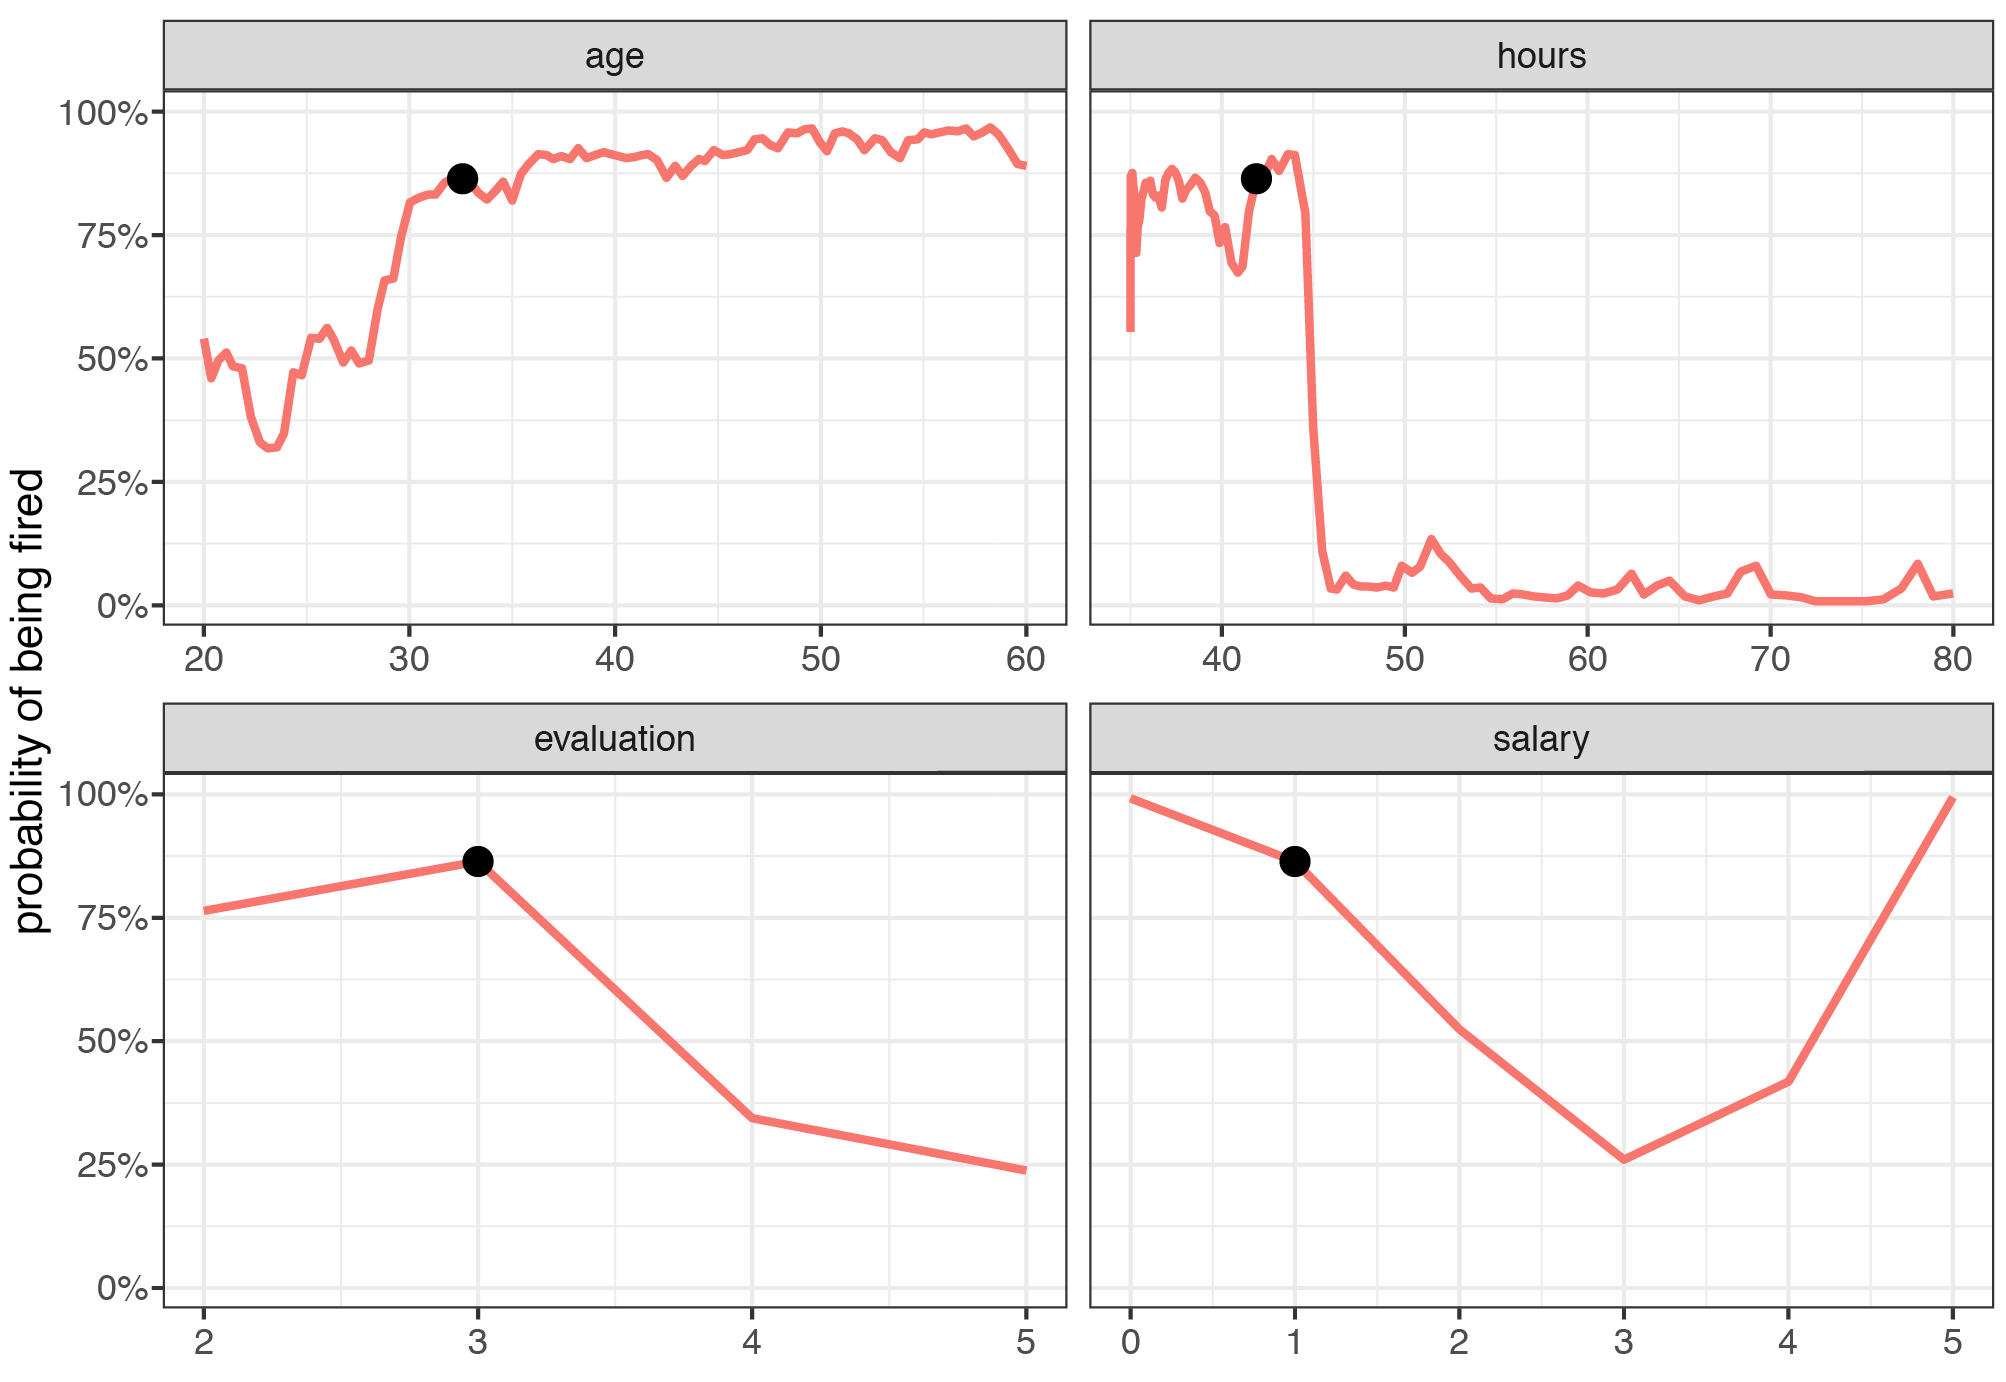
\includegraphics[width=0.7\linewidth]{figure/HR_cp_fired_all} 

}

\caption{(fig:HRCPFiredAll) Ceteris Paribus profiles for all continuous variables}\label{fig:HRCPFiredAll}
\end{figure}

\hypertarget{oscillations}{%
\subsubsection{Profile oscillations}\label{oscillations}}

Visual examination of variables is insightful, but for large number of
variables we end up with large number of panels, most of which are flat.
This is why we want to asses variable importance and show only profiles
for important variables. The advantage of CP profiles is that they lead
to a very natural and intuitive way of assessing the variable importance
for a single prediction. The intuition is: the more important variable
the larger are changes along the CP profile. If variable is not
important then model response will barely change. If variable is
important the CP profile change a lot for different values of a
variable.

Let's write it down in a more formal way.

Let \(vip^{CP}_j(x)\) denotes variable importance calculated based on CP
profiles in point \(x\) for variable \(j\).

\[
vip^{CP}_j(x) = \int_{-\inf}^{inf} |CP^{f,j,x}(z) - f(x)| dz
\]

So it's an absolute deviation from \(f(x)\). Note that one can consider
different modification of this coefficient:

\begin{enumerate}
\def\labelenumi{\arabic{enumi}.}
\tightlist
\item
  Deviations can be calculated not as a distance from \(f(x)\) but from
  average \(\bar CP^{f,j,x}(z)\).
\item
  The integral may be weighted based on the density of variable \(x^j\).
\item
  Instead of absolute deviations one may use root from average squares.
\end{enumerate}

TODO: we need to verify which approach is better. Anna Kozak is working
on this

The straightforward estimator for \(vip^{CP}_j(x)\) is

\[
\widehat{ vip^{CP}_j(x)} = \frac 1n \sum_{i=1}^n |CP^{f,j,x}(x_i) - f(x)|.
\]

Figure \ref{fig:CPVIPprofiles} shows the idea behind measuring
oscillations. The larger the highlighted area the more important is the
variable.

\begin{figure}

{\centering 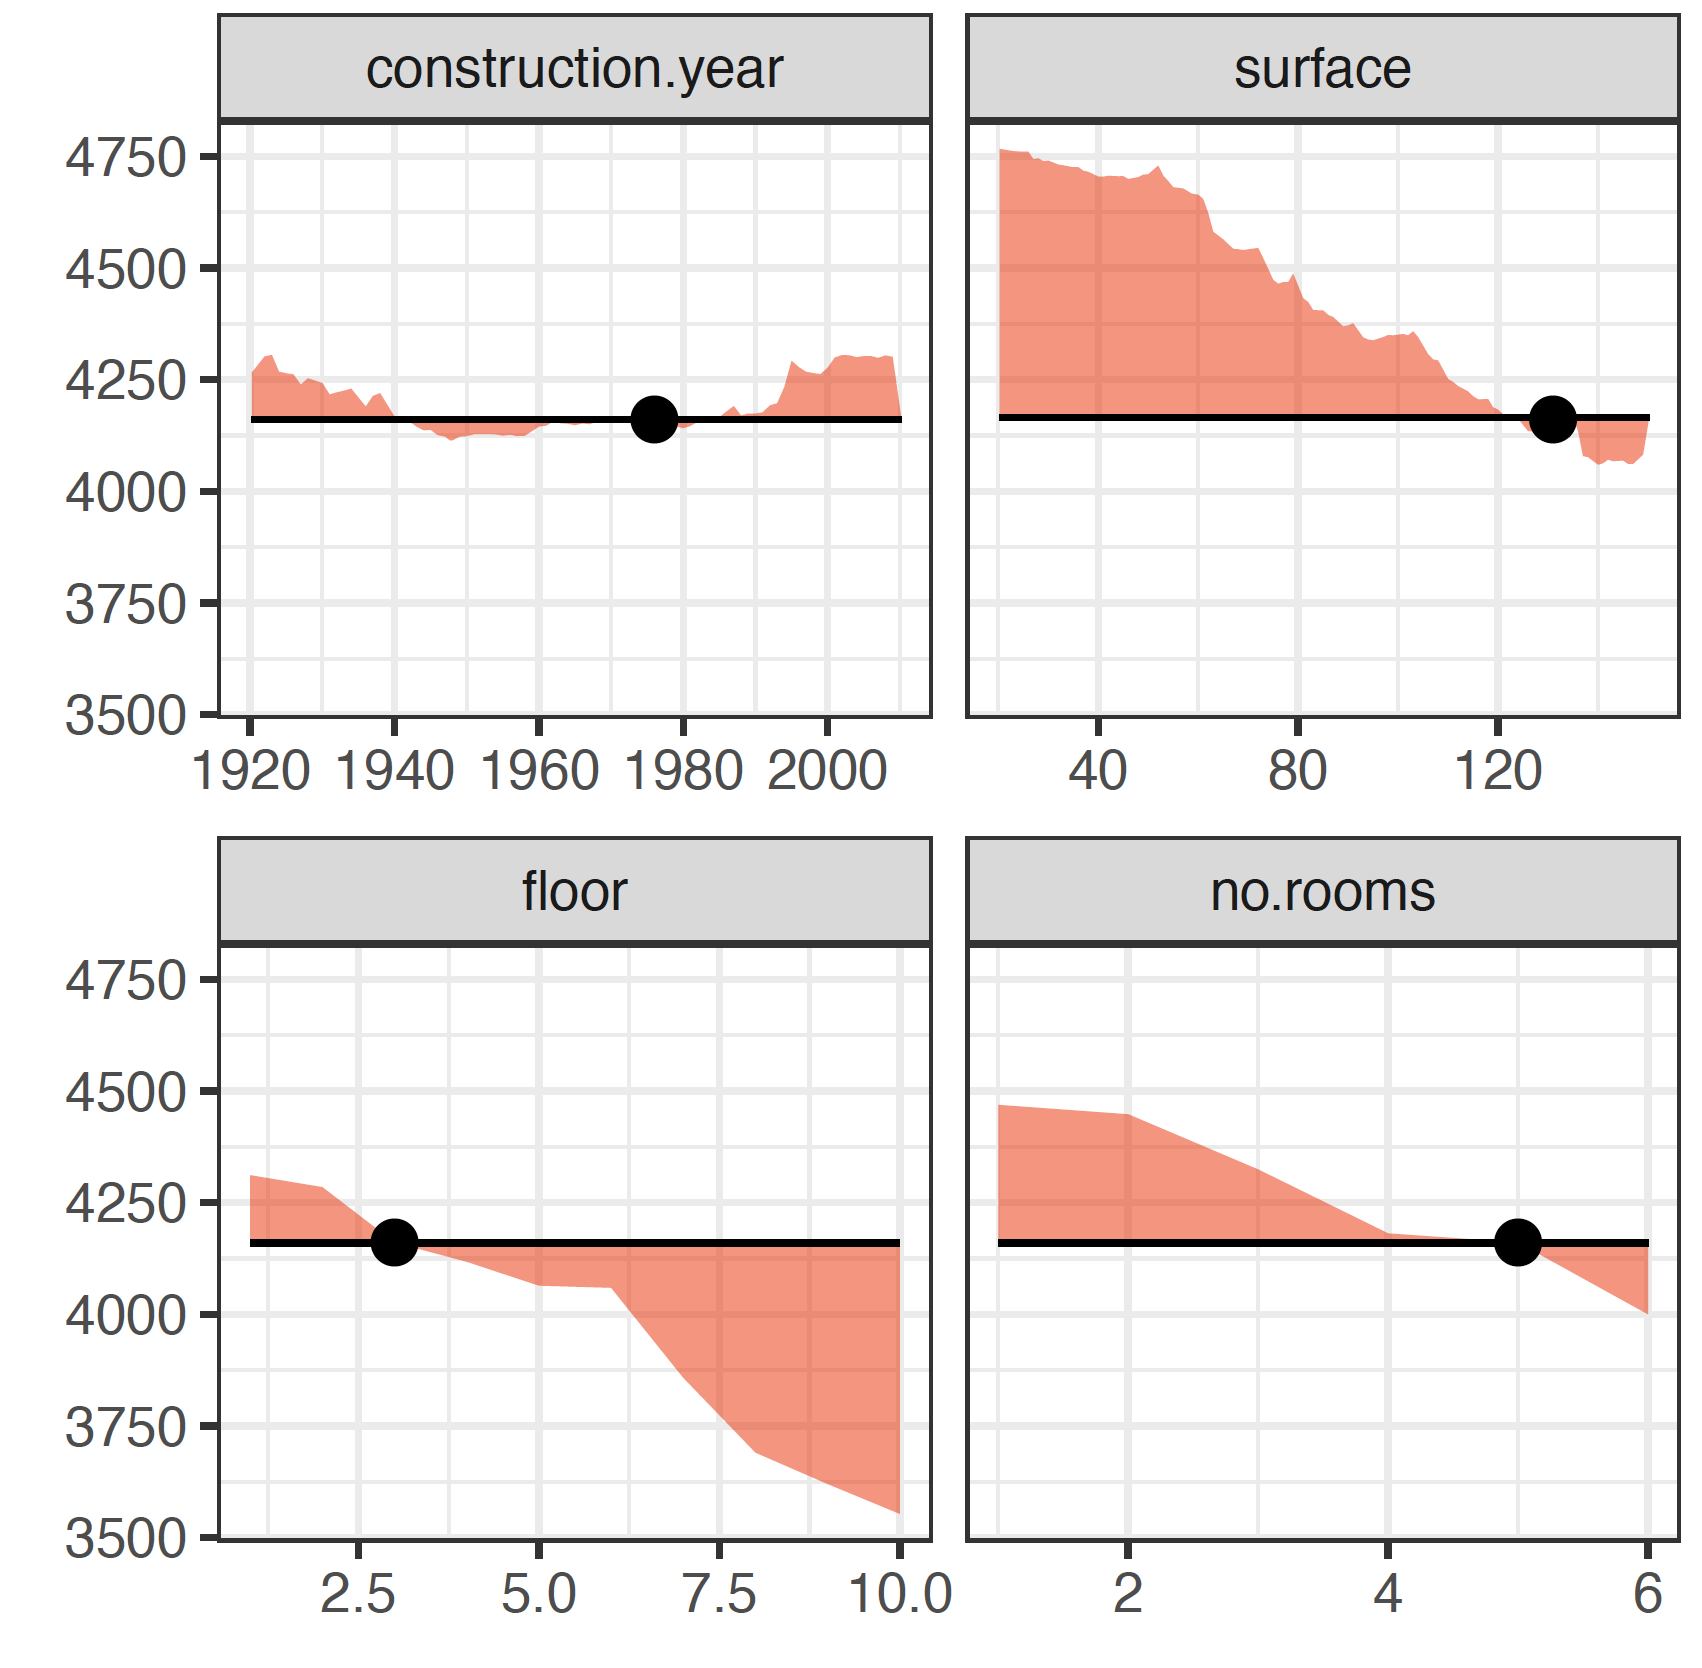
\includegraphics[width=0.5\linewidth]{figure/CP_VIP_profiles} 

}

\caption{(fig:CPVIPprofiles) CP oscillations are average deviations between CP profiles and the model response}\label{fig:CPVIPprofiles}
\end{figure}

Figure \ref{fig:CPVIP1} summarizes variable oscillations. Such visuals
help to quickly grasp how large are model oscillations around a specific
point.

\begin{figure}

{\centering 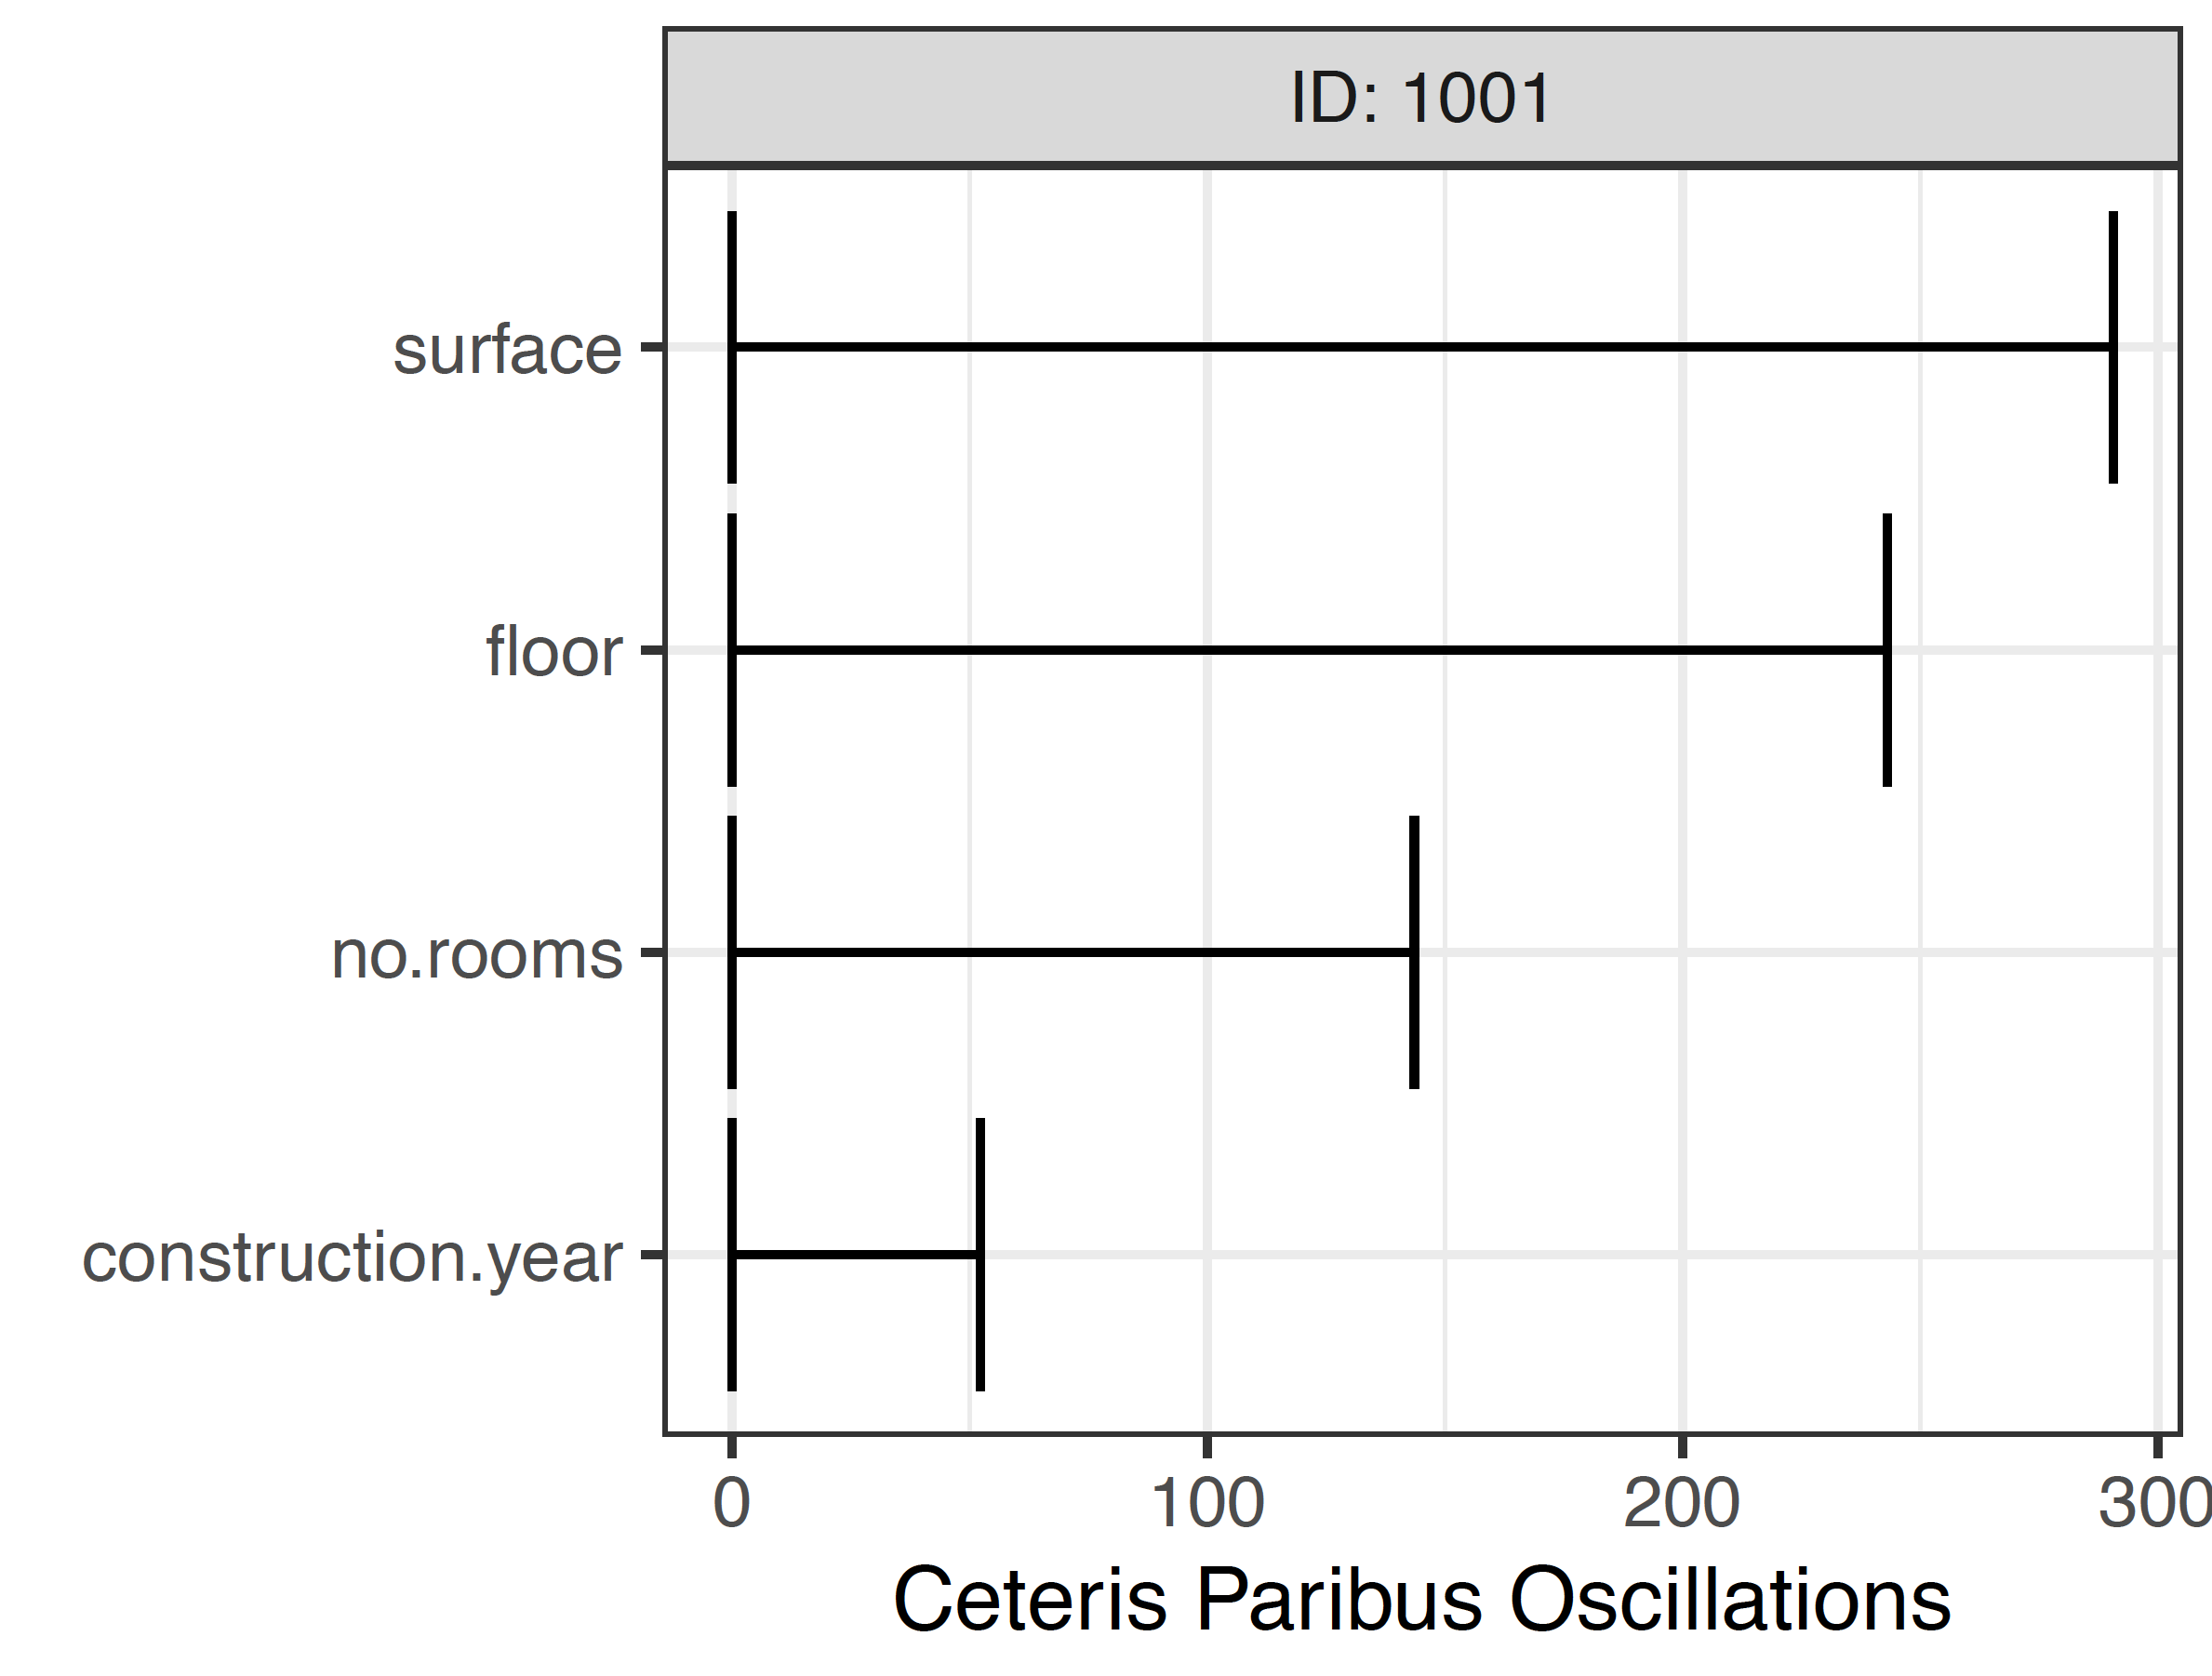
\includegraphics[width=0.4\linewidth]{figure/cp_vip_1} 

}

\caption{(fig:CPVIP1) Variable importance plots calculated for Ceteris Paribus profiles for observation ID: 1001}\label{fig:CPVIP1}
\end{figure}

\textbf{NOTE}

Variable importance for single prediction may be very different than
variable importance for the full model.

For example, consider a model \[
f(x_1, x_2) = x_1 * x_2
\] where variables \(x_1\) and \(x_2\) takes values in \([0,1]\).

From the global perspective both variables are equally important.

But local variable importance is very different. Around point
\(x = (0, 1)\) the importance of \(x_1\) is much larger than \(x_2\).
This is because profile for \(f(z, 1)\) have larger oscillations than
\(f(0, z)\).

\hypertarget{d-profiles}{%
\subsubsection{2D profiles}\label{d-profiles}}

The definition of ceteris paribus profiles given in section
\ref{ceterisParibus1d} may be easily extended to two and more variables.
Also definition of CP oscillations \ref{oscillations} have straight
forward generalization for larger number of dimensions. Such
generalisations are usefull when model is non additive. Presence of
pairwise interactions may be detected with 2D Ceteris Paribus plots.

Let's define two-dimensional Ceteris Paribus Profile for model \(f\),
variables \(j\) and \(k\) and point \(x\) as

\[
CP^{f, (j,k), x}(z_1, z_2) := f(x|^{(j,k)} = (z_1,z_2)).
\] I.e. CP profile is a model response obtained for observations created
based on \(x\) with \(j\) and \(k\) coordinates changed to
\((z_1, z_2)\) and all other coordinates kept unchanged.

A natural way to visualise 2D CP profiles is to use a level plot as in
Figure \ref{fig:CP2Dsurflor}.

\begin{figure}

{\centering 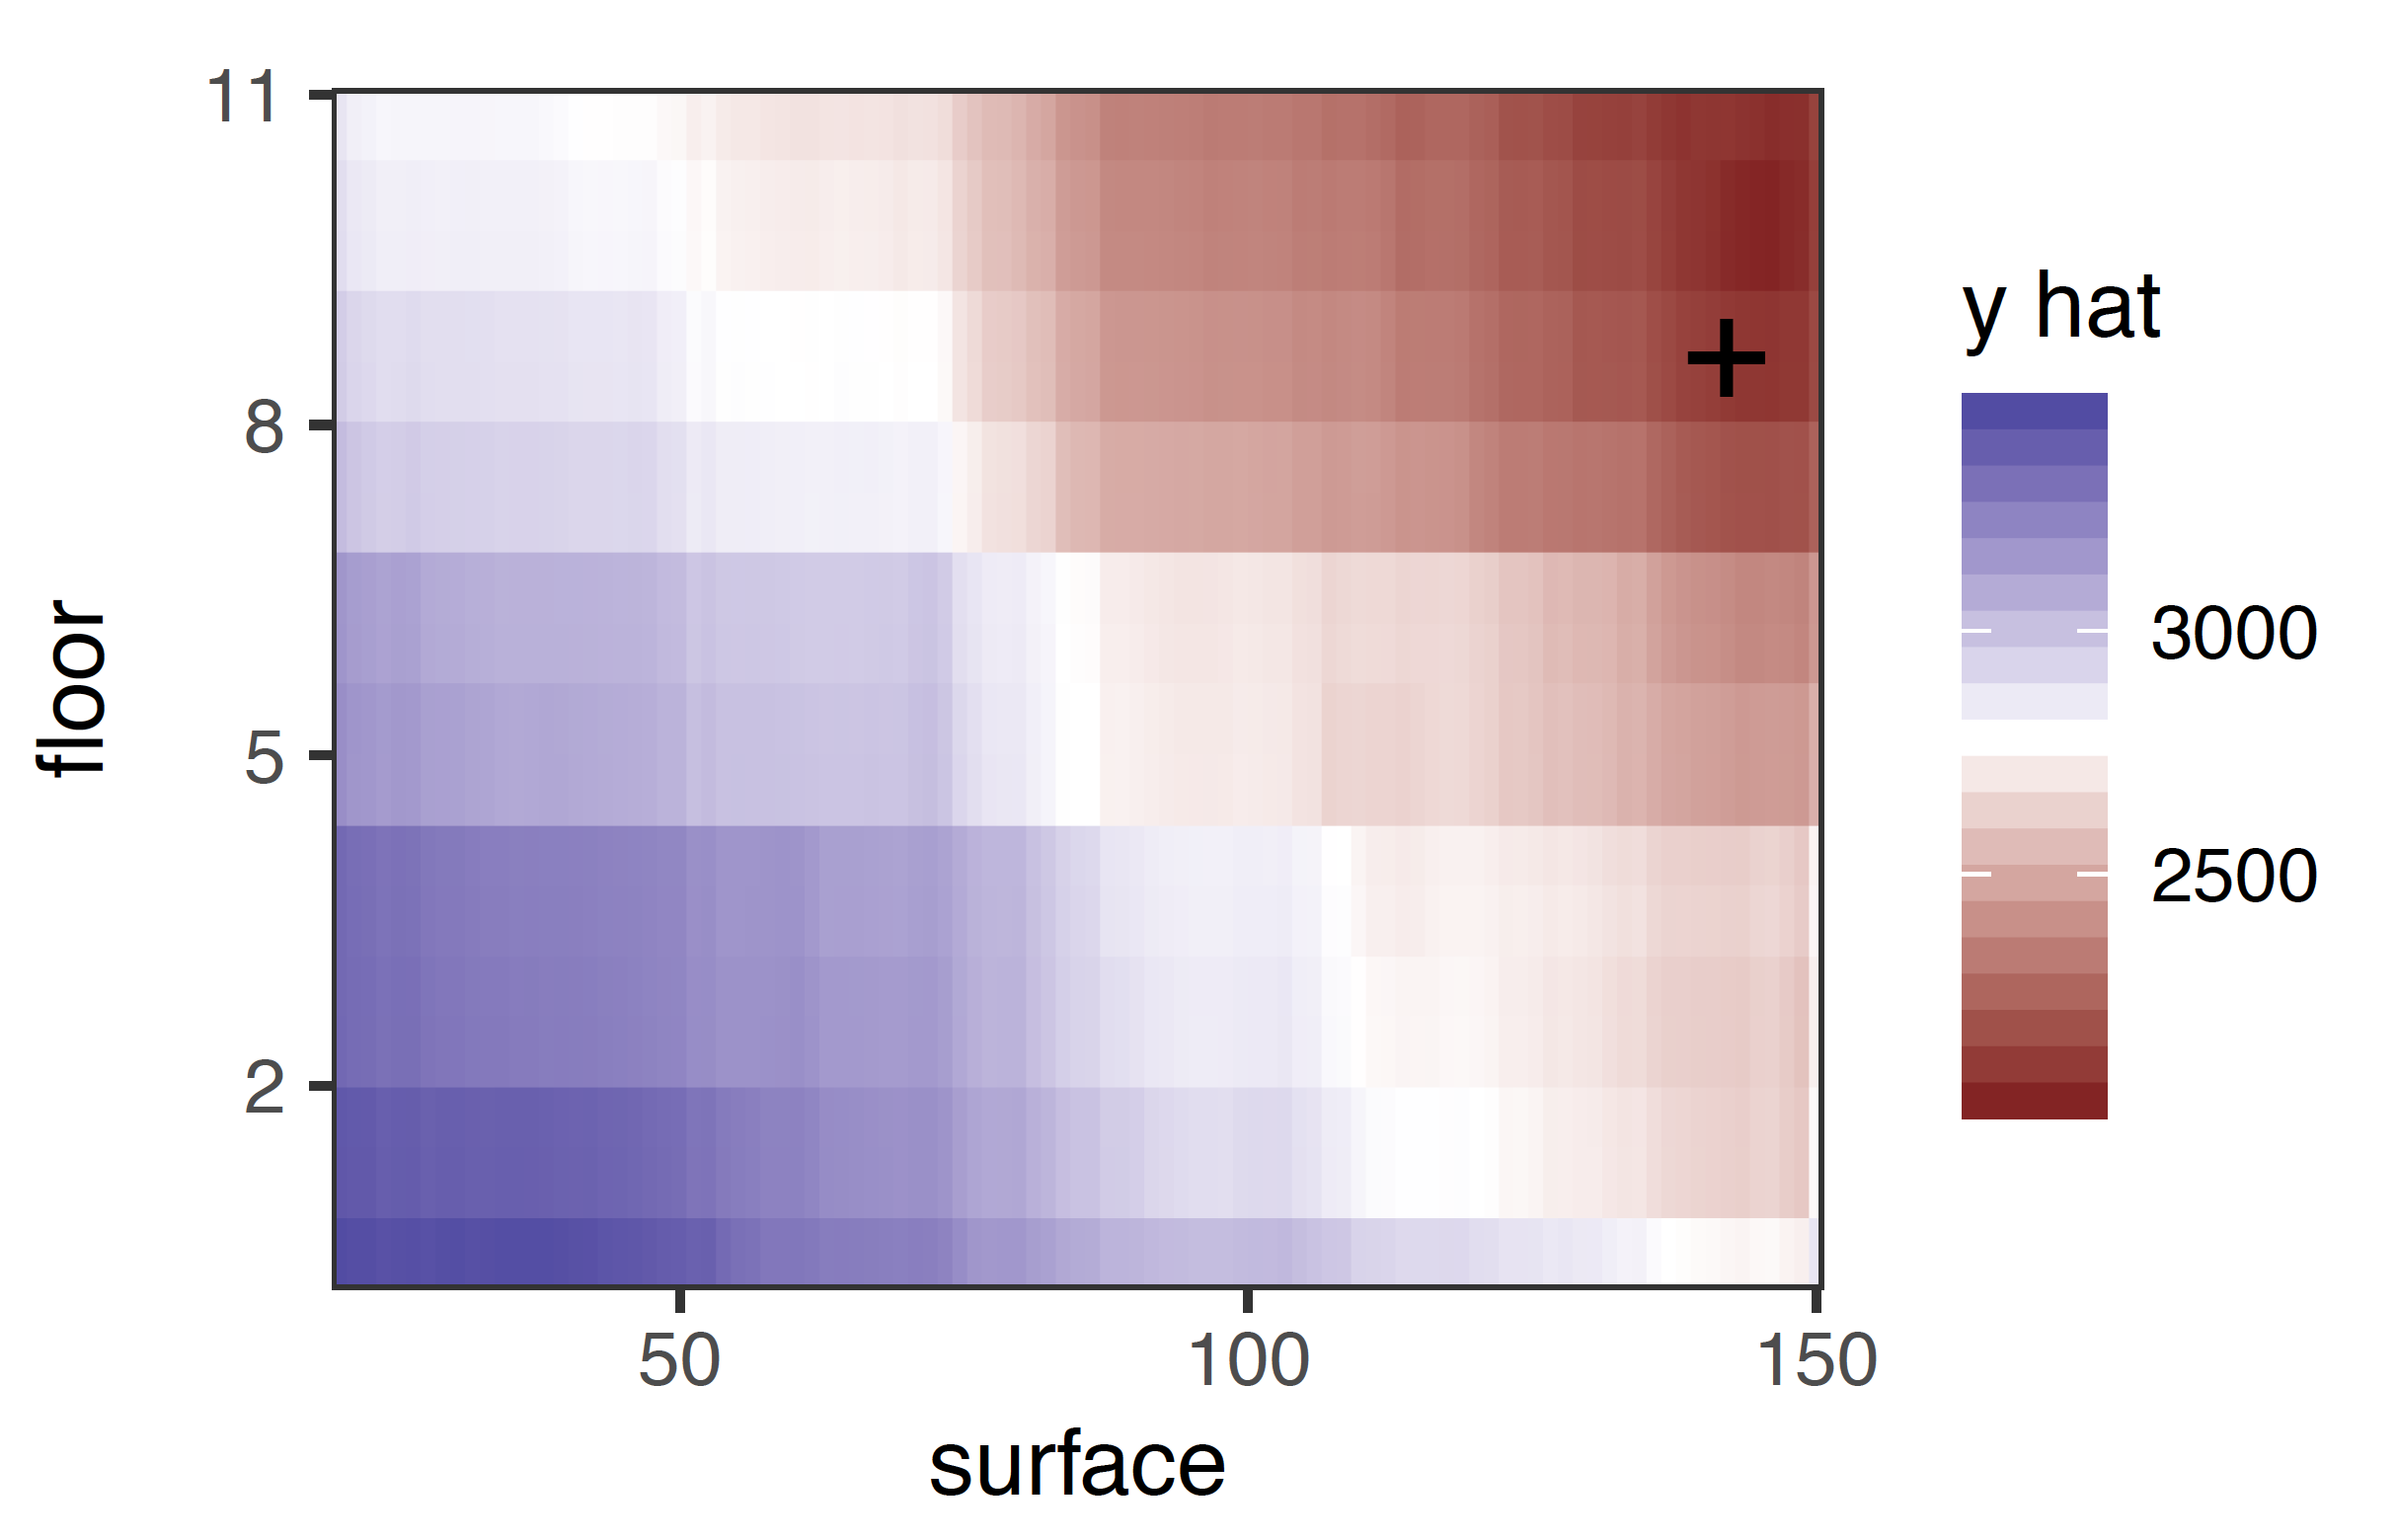
\includegraphics[width=0.6\linewidth]{figure/cp_2d_surf_floor} 

}

\caption{(fig:CP2Dsurflor) Ceteris Paribus plot for a pair of variales. Black cross marks coordinated for the observation of interest. Presented model estimates price of an appartment}\label{fig:CP2Dsurflor}
\end{figure}

If number of variables is small or moderate thein it is possible to
present all pairs of variables. See an example in Figure
\ref{fig:CP2Dall}.

\begin{figure}

{\centering 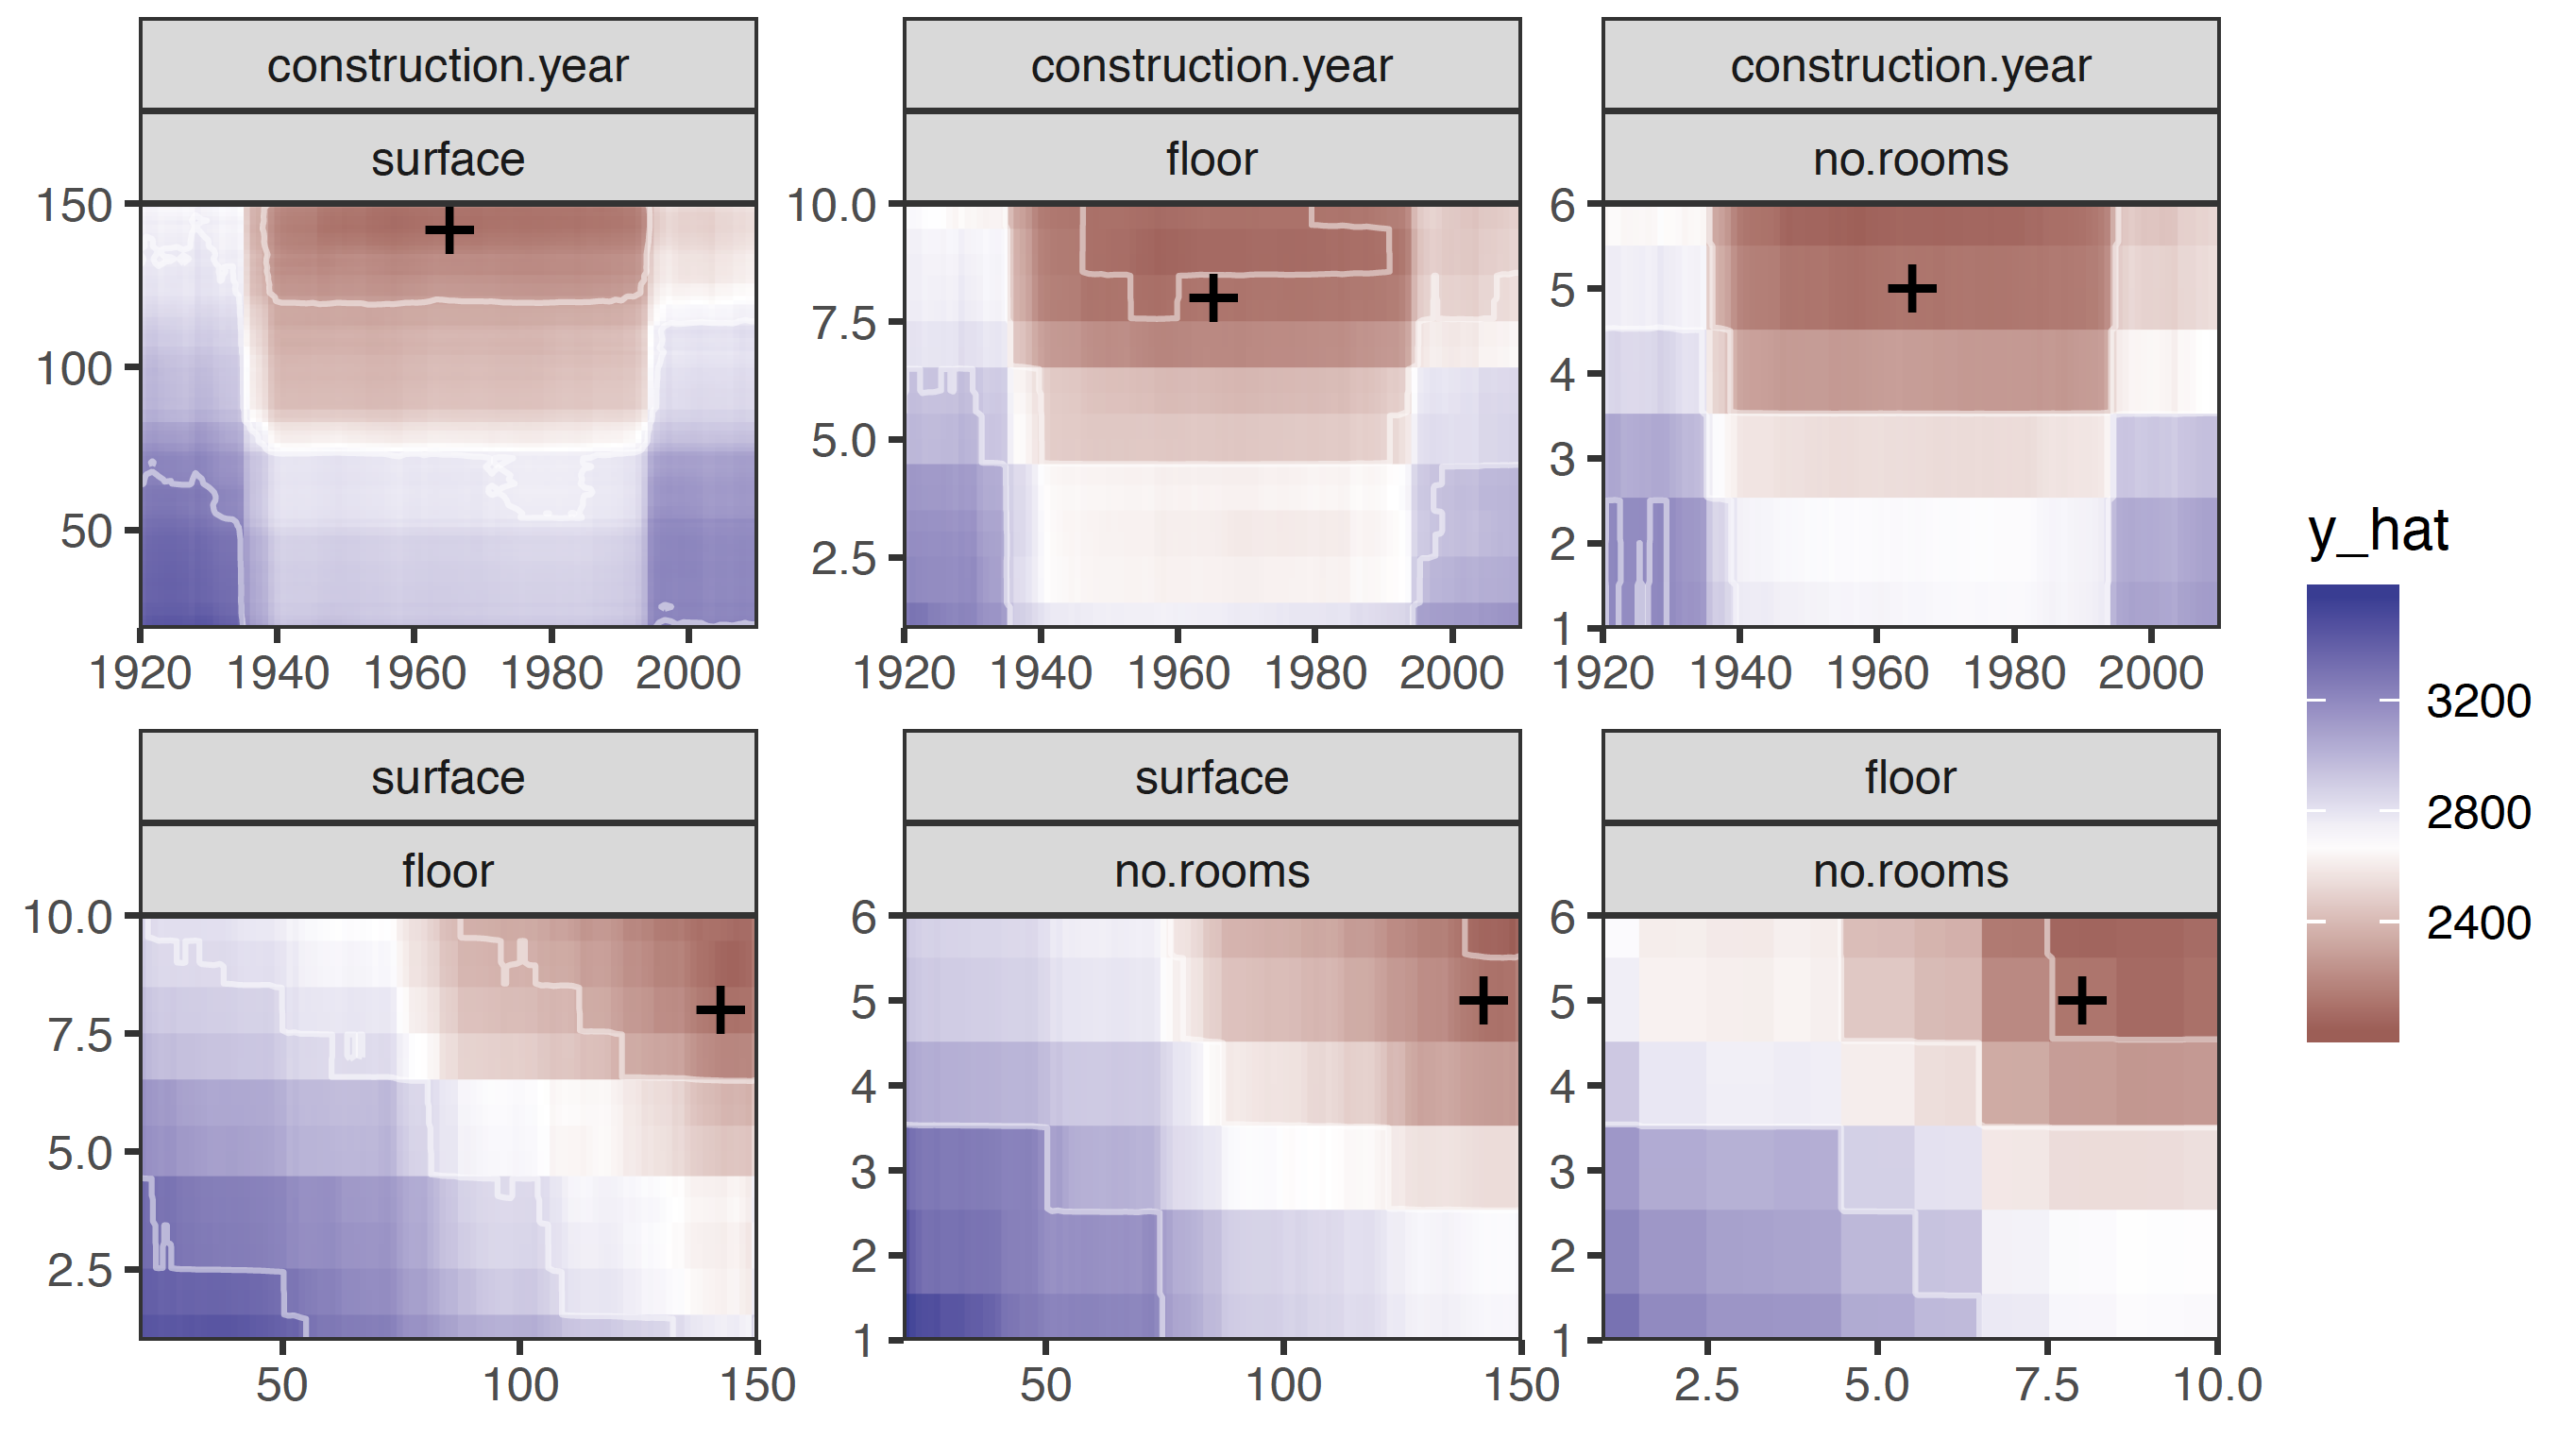
\includegraphics[width=0.9\linewidth]{figure/cp_2d_all} 

}

\caption{(fig:CP2Dall) Ceteris Paribus plot for all pairs of variales.}\label{fig:CP2Dall}
\end{figure}

\hypertarget{local-model-fidelity}{%
\subsection{Local model fidelity}\label{local-model-fidelity}}

Ceteris Paribus profiles are also a useful tool to validate local model
fidelity. It may happen that global performance of the model is good,
while for some points the local fit is very bad. Local fidelity helps to
understand how good is the model fit around point of interest.

How does it work?

The idea behind fidelity plots is to select some number of points from
the validation dataset that are closes to the point of interest. It's a
similar approach as in k nearest neighbours. Then for these neighbours
we may plot Ceteris Paribus Profiles and check how stable they are.

Also, if we know true taget values for points from the validation
dataset we may plot residuals to show how large are residuals.

An example fidelity plot is presented in Figure \ref{fig:CPfidelity1}.
Black line shows the CP profiles for the point of interest, while grey
lines show CP profiles for neihgbors. Red intervals stand for residuals
and in this example it looks like residuals for neighbours are all
negative. Thus maybe model is biased around the point of interest.

\begin{figure}

{\centering 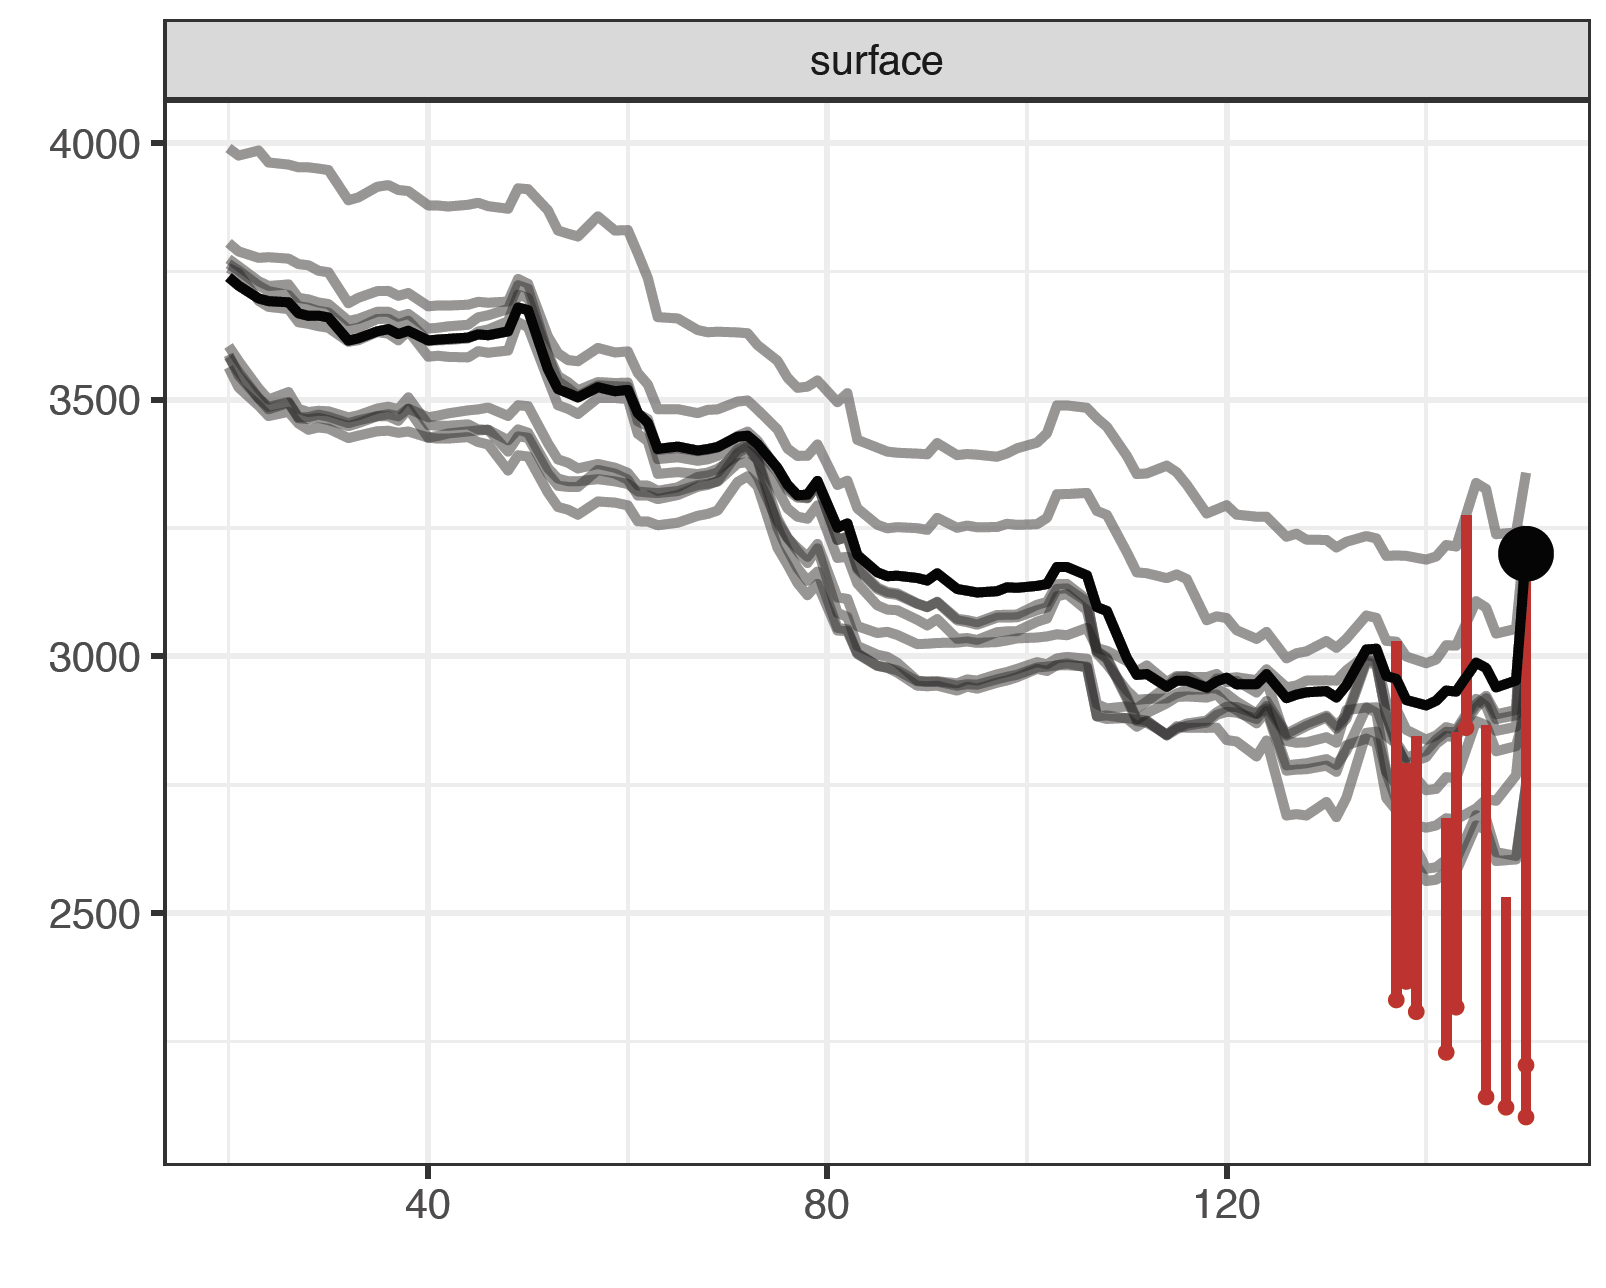
\includegraphics[width=0.7\linewidth]{figure/cp_fidelity_1} 

}

\caption{(fig:CPfidelity1) Local fidelity plots. Black line shows the CP profile for the point of interest. Grey lines show CP profiles for nearest neighbors. Red intervals correspond to residuals. Each red interval starts in a model prediction for a selected neighbor and ends in its true value of target variable.}\label{fig:CPfidelity1}
\end{figure}

This observation may be confirmed by plots that compare distribution of
all residuals against distribution of residuals for neighbors.

See Figure \ref{fig:CPfidelityBoxplot} for an example. Here residuals
for neighbors are shifted towards highest values. This suggests that the
model response is biased around the observation of interest.

TODO: diagnostic score: average quantaile of neighbours.

\begin{figure}

{\centering 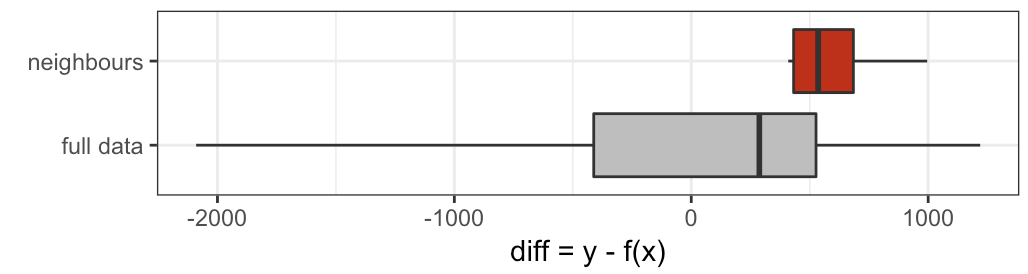
\includegraphics[width=0.7\linewidth]{figure/cp_fidelity_boxplot} 

}

\caption{(fig:CPfidelityBoxplot) Distribution of residuals for whole validation data (grey boxplot) and for selected closes 15 neighbors (red boxplot).}\label{fig:CPfidelityBoxplot}
\end{figure}

\hypertarget{example}{%
\subsection{Example}\label{example}}

\hypertarget{pros-and-cons-5}{%
\subsection{Pros and cons}\label{pros-and-cons-5}}

Ceteris Paribus principle gives a uniform and extendable approach to
model exploration. Below we summarize key strengths and weaknesses of
this approach.

\textbf{Pros}

\begin{itemize}
\tightlist
\item
  Graphical representation of Ceteris Paribus profile is easy to
  understand.
\item
  Ceteris Paribus profiles are compact and it is easy to fit many models
  or many variables in a small space.
\item
  Ceteris Paribus profiles helps to understand how model response would
  change and how stable it is
\item
  Oscillations calculated for CP profiles helps to select the most
  important variables.
\item
  2D Ceteris Paribus profiles help to identify pairwise interactions
  between variables.
\end{itemize}

\textbf{Cons}

\begin{itemize}
\tightlist
\item
  If variables are correlated (like surface and number of rooms) then
  the `\emph{everything else kept unchanged}' approach leads to
  unrealistic settings.
\item
  Interactions between variables are not visible in 1D plots.
\item
  This tool is not suited for very wide data, like hundreds or thousands
  of variables.
\item
  Visualization of categorical variables is non trivial.
\end{itemize}

\hypertarget{code-snippets-for-r-4}{%
\subsection{Code snippets for R}\label{code-snippets-for-r-4}}

In this section we present key features of the \texttt{ceterisParibus}
package for R \citep{R-ceterisParibus}. This package covers all features
presented in this chapter. It is available on CRAN and GitHub. Find more
examples at the website of this package
\texttt{https://pbiecek.github.io/ceterisParibus/}.

A very interesting tool for moedl explorartion with similar principle is
implemented in the \texttt{condvis} package \citep{JSSv081i05}.

\textbf{Model preparation}

In this section we will present examples based on the
\texttt{apartments} dataset. See section TODO for more details.

\begin{Shaded}
\begin{Highlighting}[]
\KeywordTok{library}\NormalTok{(}\StringTok{"DALEX"}\NormalTok{)}
\KeywordTok{head}\NormalTok{(apartments)}
\end{Highlighting}
\end{Shaded}

\begin{verbatim}
##   m2.price construction.year surface floor no.rooms    district
## 1     5897              1953      25     3        1 Srodmiescie
## 2     1818              1992     143     9        5     Bielany
## 3     3643              1937      56     1        2       Praga
## 4     3517              1995      93     7        3      Ochota
## 5     3013              1992     144     6        5     Mokotow
## 6     5795              1926      61     6        2 Srodmiescie
\end{verbatim}

The problem here is to predict average price for square meter for an
apartment. Let's build a random forest model with \texttt{randomForest}
package \citep{R-randomForest}.

\begin{Shaded}
\begin{Highlighting}[]
\KeywordTok{library}\NormalTok{(}\StringTok{"randomForest"}\NormalTok{)}
\NormalTok{rf_model <-}\StringTok{ }\KeywordTok{randomForest}\NormalTok{(m2.price }\OperatorTok{~}\StringTok{ }\NormalTok{construction.year }\OperatorTok{+}\StringTok{ }\NormalTok{surface }\OperatorTok{+}\StringTok{ }\NormalTok{floor }\OperatorTok{+}
\StringTok{      }\NormalTok{no.rooms, }\DataTypeTok{data =}\NormalTok{ apartments)}
\NormalTok{rf_model}
\end{Highlighting}
\end{Shaded}

\begin{verbatim}
## 
## Call:
##  randomForest(formula = m2.price ~ construction.year + surface +      floor + no.rooms, data = apartments) 
##                Type of random forest: regression
##                      Number of trees: 500
## No. of variables tried at each split: 1
## 
##           Mean of squared residuals: 485330.8
##                     % Var explained: 40.9
\end{verbatim}

Model exploration with \texttt{ceterisParibus} package is performed in
four steps.

\textbf{1. Create an explainer - wrapper around model and validation
data.}

Since all other functions work in a model agnostic fashion, first we
need to define a wrapper around the model. Here we are using the
\texttt{explain()} function from \texttt{DALEX} package \citep{R-DALEX}.

\begin{Shaded}
\begin{Highlighting}[]
\KeywordTok{library}\NormalTok{(}\StringTok{"DALEX"}\NormalTok{)}
\NormalTok{explainer_rf <-}\StringTok{ }\KeywordTok{explain}\NormalTok{(rf_model,}
      \DataTypeTok{data =}\NormalTok{ apartmentsTest, }\DataTypeTok{y =}\NormalTok{ apartmentsTest}\OperatorTok{$}\NormalTok{m2.price)}
\NormalTok{explainer_rf}
\end{Highlighting}
\end{Shaded}

\begin{verbatim}
## Model label:  randomForest 
## Model class:  randomForest.formula,randomForest 
## Data head  :
##      m2.price construction.year surface floor no.rooms    district
## 1001     4644              1976     131     3        5 Srodmiescie
## 1002     3082              1978     112     9        4     Mokotow
\end{verbatim}

\textbf{2. Define point of interest.}

Certeris Paribus profiles explore model around a single point.

\begin{Shaded}
\begin{Highlighting}[]
\NormalTok{new_apartment <-}\StringTok{ }\KeywordTok{data.frame}\NormalTok{(}\DataTypeTok{construction.year =} \DecValTok{1965}\NormalTok{, }\DataTypeTok{no.rooms =} \DecValTok{5}\NormalTok{, }\DataTypeTok{surface =} \DecValTok{142}\NormalTok{, }\DataTypeTok{floor =} \DecValTok{8}\NormalTok{)}
\NormalTok{new_apartment}
\end{Highlighting}
\end{Shaded}

\begin{verbatim}
##   construction.year no.rooms surface floor
## 1              1965        5     142     8
\end{verbatim}

\begin{Shaded}
\begin{Highlighting}[]
\KeywordTok{predict}\NormalTok{(rf_model, new_apartment)}
\end{Highlighting}
\end{Shaded}

\begin{verbatim}
##        1 
## 2341.367
\end{verbatim}

\textbf{3. Calculate CP profiles}

The \texttt{ceteris\_paribus()} function calculates CP profiles for
selected model around selected observation.

By default CP profiles are calculated for all numerical variables. Use
the \texttt{variables} argument to select subset of interesting
variables. The result from \texttt{ceteris\_paribus()}function is a data
frame with model predictions for modified points around the point of
interest.

\begin{Shaded}
\begin{Highlighting}[]
\KeywordTok{library}\NormalTok{(}\StringTok{"ceterisParibus"}\NormalTok{)}
\NormalTok{cp_rf <-}\StringTok{ }\KeywordTok{ceteris_paribus}\NormalTok{(explainer_rf, new_apartment, }
                            \DataTypeTok{variables =} \KeywordTok{c}\NormalTok{(}\StringTok{"construction.year"}\NormalTok{, }\StringTok{"floor"}\NormalTok{))}
\NormalTok{cp_rf}
\end{Highlighting}
\end{Shaded}

\begin{verbatim}
## Top profiles    : 
##     construction.year no.rooms surface floor   _yhat_           _vname_
## 1                1920        5     142     8 3102.043 construction.year
## 1.1              1921        5     142     8 3132.637 construction.year
## 1.2              1922        5     142     8 3118.195 construction.year
## 1.3              1923        5     142     8 3090.137 construction.year
## 1.4              1924        5     142     8 3101.309 construction.year
## 1.5              1925        5     142     8 3115.526 construction.year
##     _ids_      _label_
## 1       1 randomForest
## 1.1     1 randomForest
## 1.2     1 randomForest
## 1.3     1 randomForest
## 1.4     1 randomForest
## 1.5     1 randomForest
## 
## 
## Top observations:
##   construction.year no.rooms surface floor   _yhat_      _label_ _ids_
## 1              1965        5     142     8 2341.367 randomForest     1
\end{verbatim}

\textbf{4. Plot CP profiles.}

Generic \texttt{plot()} function plot CP profiles. It returns a
\texttt{ggplot2} object that can be polished if needed. Use additional
arguments of this function to select colors and sizes for elements
visible in the plot.

\begin{Shaded}
\begin{Highlighting}[]
\KeywordTok{plot}\NormalTok{(cp_rf) }
\end{Highlighting}
\end{Shaded}

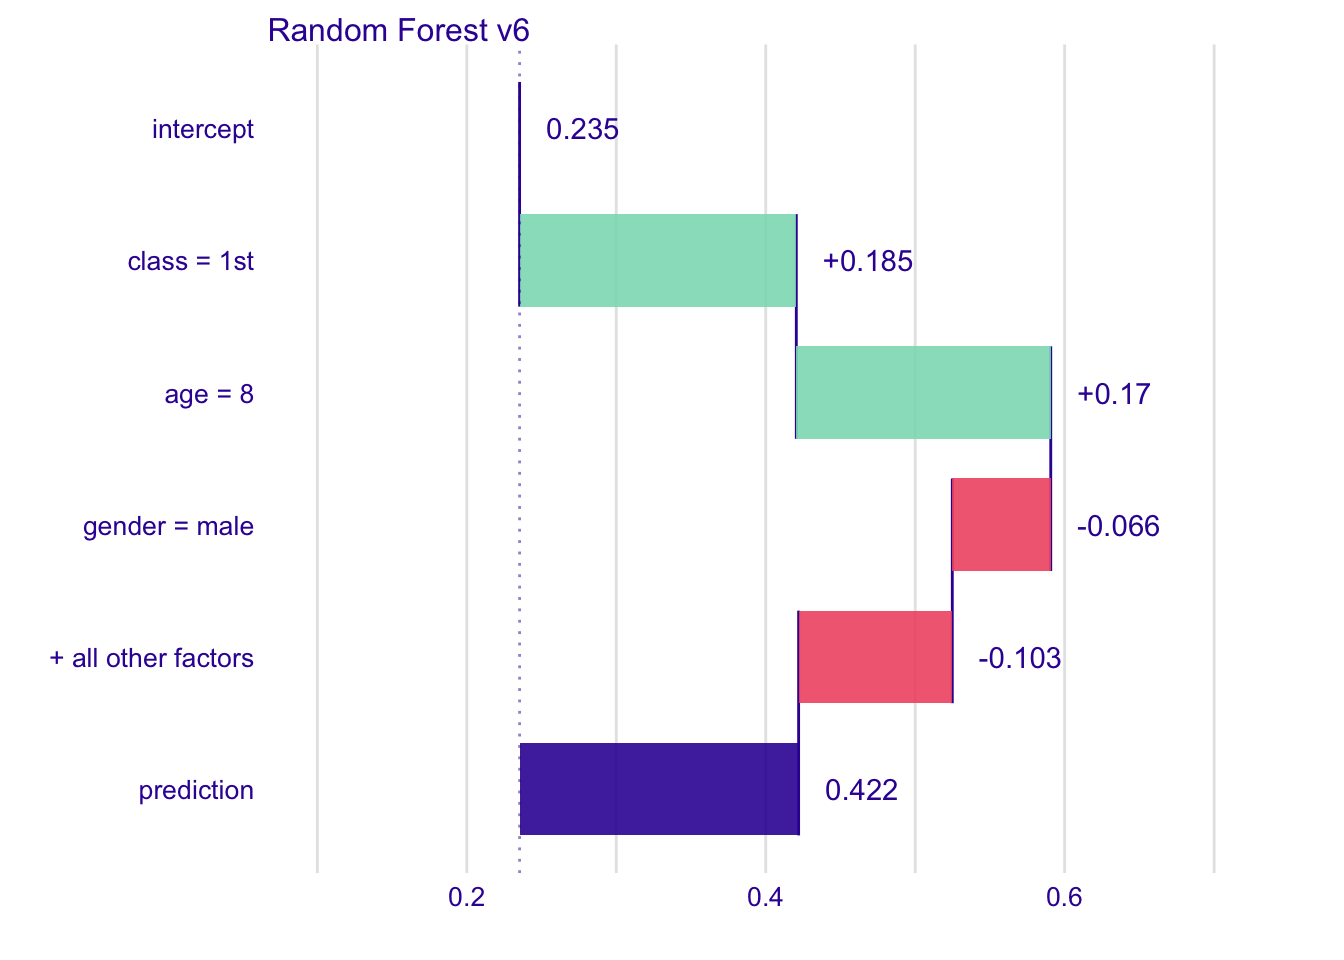
\includegraphics{PM_VEE_files/figure-latex/unnamed-chunk-34-1.pdf}

One of very useful features of \texttt{ceterisParibus} explainers is
that profiles for two or more models may be superimposed in a single
plot. This helps in model comparisons.

Let's create a linear model for this dataset and repeat steps 1-3 for
the lm model.

\begin{Shaded}
\begin{Highlighting}[]
\NormalTok{lm_model <-}\StringTok{ }\KeywordTok{lm}\NormalTok{(m2.price }\OperatorTok{~}\StringTok{ }\NormalTok{construction.year }\OperatorTok{+}\StringTok{ }\NormalTok{surface }\OperatorTok{+}\StringTok{ }\NormalTok{floor }\OperatorTok{+}
\StringTok{      }\NormalTok{no.rooms, }\DataTypeTok{data =}\NormalTok{ apartments)}
\NormalTok{explainer_lm <-}\StringTok{ }\KeywordTok{explain}\NormalTok{(lm_model,}
      \DataTypeTok{data =}\NormalTok{ apartmentsTest, }\DataTypeTok{y =}\NormalTok{ apartmentsTest}\OperatorTok{$}\NormalTok{m2.price)}
\NormalTok{cp_lm <-}\StringTok{ }\KeywordTok{ceteris_paribus}\NormalTok{(explainer_lm, new_apartment, }
                            \DataTypeTok{variables =} \KeywordTok{c}\NormalTok{(}\StringTok{"construction.year"}\NormalTok{, }\StringTok{"floor"}\NormalTok{))}
\end{Highlighting}
\end{Shaded}

Now we can use function \texttt{plot()} to compare both models in a
single chart. Additional argument \texttt{color\ =\ "\_label\_"} set
color as a key for model.

\begin{Shaded}
\begin{Highlighting}[]
\KeywordTok{plot}\NormalTok{(cp_rf, cp_lm, }\DataTypeTok{color =} \StringTok{"_label_"}\NormalTok{)}
\end{Highlighting}
\end{Shaded}

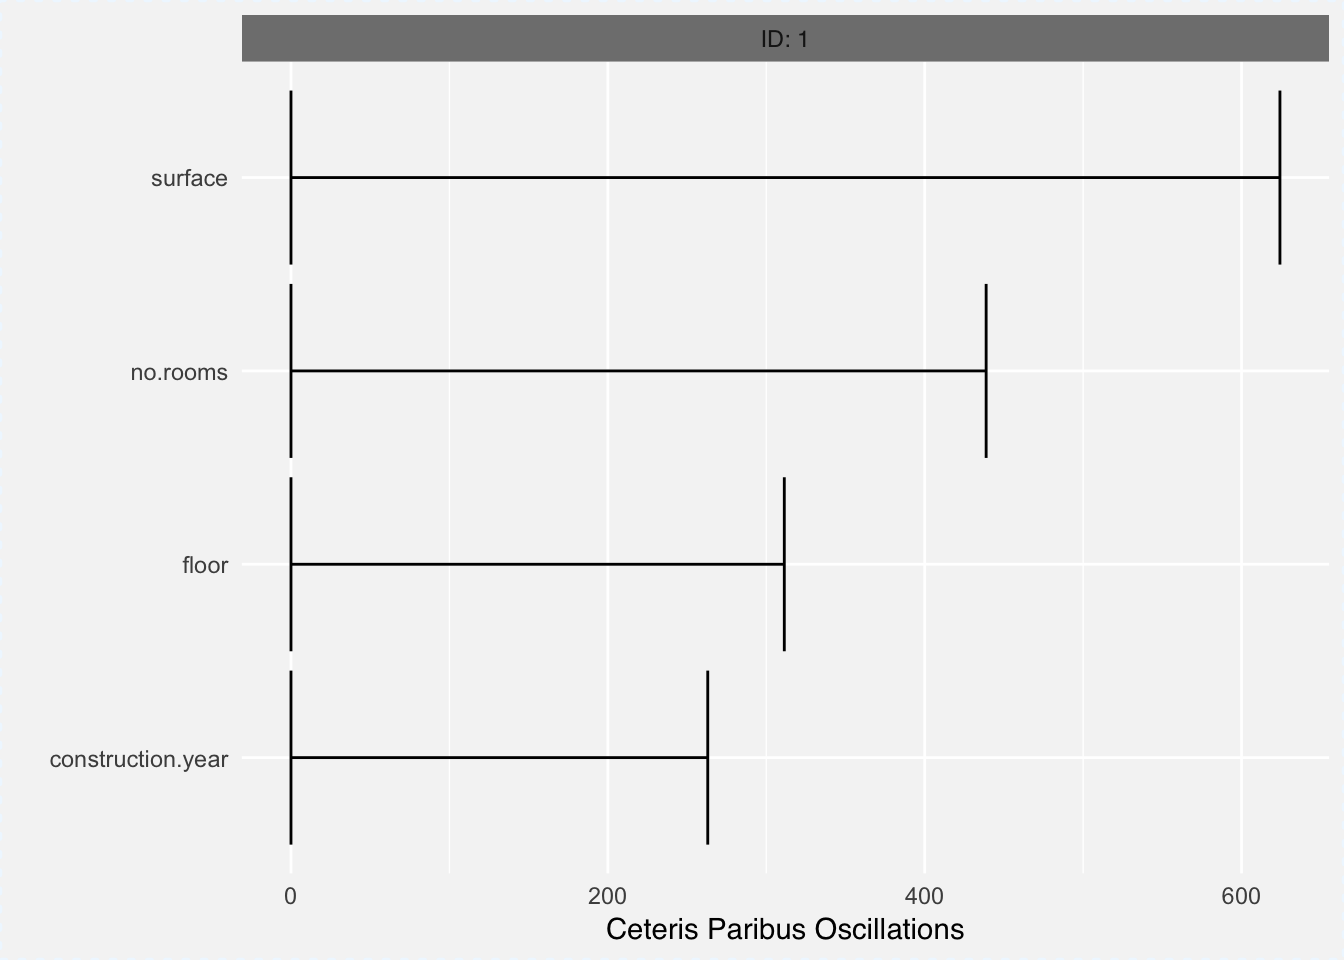
\includegraphics{PM_VEE_files/figure-latex/unnamed-chunk-36-1.pdf}

\textbf{Oscillations}

The \texttt{calculate\_oscillations()} function calculates oscillations
for CP profiles.

\begin{Shaded}
\begin{Highlighting}[]
\NormalTok{cp_rf_all <-}\StringTok{ }\KeywordTok{ceteris_paribus}\NormalTok{(explainer_rf, new_apartment)}
\NormalTok{co_rf_all <-}\StringTok{ }\KeywordTok{calculate_oscillations}\NormalTok{(cp_rf_all)}
\NormalTok{co_rf_all}
\end{Highlighting}
\end{Shaded}

\begin{verbatim}
##             _vname_ _ids_ oscillations
## 3           surface     1     608.0858
## 2          no.rooms     1     415.7131
## 4             floor     1     316.5819
## 1 construction.year     1     241.1452
\end{verbatim}

\begin{Shaded}
\begin{Highlighting}[]
\KeywordTok{plot}\NormalTok{(co_rf_all)}
\end{Highlighting}
\end{Shaded}

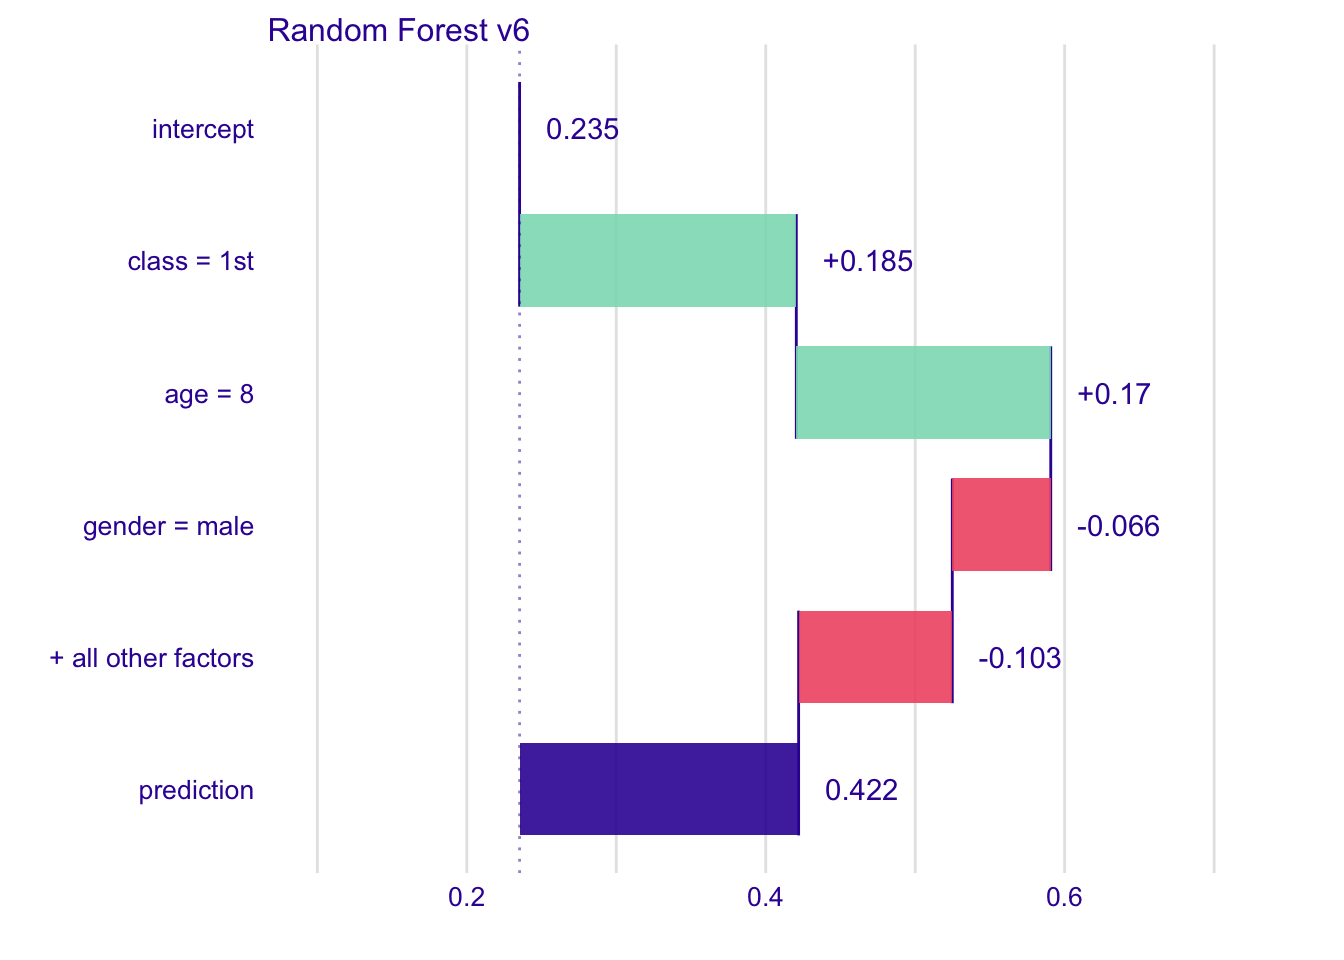
\includegraphics{PM_VEE_files/figure-latex/unnamed-chunk-37-1.pdf}

\textbf{2D Ceteris Paribus profiles}

And the \texttt{what\_if\_2d()} function calculates 2D CP profiles.

\begin{Shaded}
\begin{Highlighting}[]
\NormalTok{wi_rf_2d <-}\StringTok{ }\KeywordTok{what_if_2d}\NormalTok{(explainer_rf, }\DataTypeTok{observation =}\NormalTok{ new_apartment, }
                 \DataTypeTok{selected_variables =} \KeywordTok{c}\NormalTok{(}\StringTok{"surface"}\NormalTok{,}\StringTok{"floor"}\NormalTok{, }\StringTok{"construction.year"}\NormalTok{))}
\KeywordTok{plot}\NormalTok{(wi_rf_2d, }\DataTypeTok{split_ncol =} \DecValTok{2}\NormalTok{)}
\end{Highlighting}
\end{Shaded}

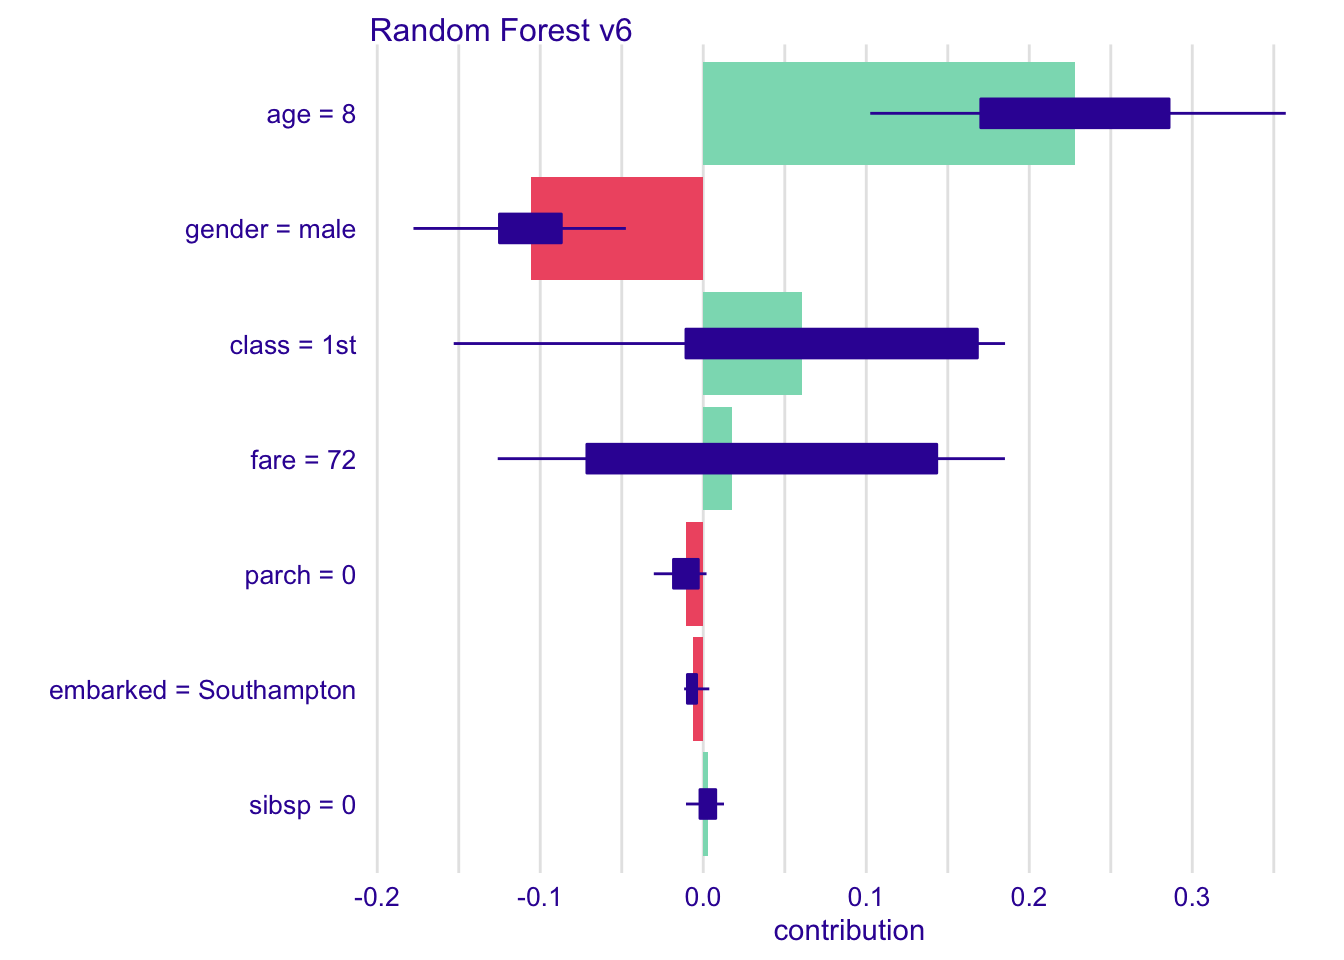
\includegraphics{PM_VEE_files/figure-latex/unnamed-chunk-38-1.pdf}

\hypertarget{comparision-of-prediction-level-explainers}{%
\section{Comparision of prediction level
explainers}\label{comparision-of-prediction-level-explainers}}

TODO

compare pros and cons of different techniques

\hypertarget{when-to-use}{%
\subsection{When to use?}\label{when-to-use}}

There are several use-cases for such explainers. Think about following.

\begin{itemize}
\tightlist
\item
  Model improvement. If model works particular bad for a selected
  observation (the residual is very high) then investigation of model
  responses for miss fitted points may give some hints how to improve
  the model. For individual predictions it is easier to notice that
  selected variable should have different a effect.
\item
  Additional domain specific validation. Understanding which factors are
  important for model predictions helps to be critical about model
  response. If model contributions are against domain knowledge then we
  may be more skeptical and willing to try another model. On the other
  hand, if the model response is aligned with domain knowledge we may
  trust more in these responses. Such trust is important in decisions
  that may lead to serious consequences like predictive models in
  medicine.
\item
  Model selection. Having multiple candidate models one may select the
  final response based on model explanations. Even if one model is
  better in terms of global model performance it may happen that locally
  other model is better fitted. This moves us towards model
  consultations that identify different options and allow human to
  select one of them.
\end{itemize}

Enslaving the Algorithm: From a `Right to an Explanation' to a `Right to
Better Decisions'? \citep{Edwards_Veale_2018}

TODO: Sparse model approximation / variable selection / feature ranking

\hypertarget{model-level-explanations}{%
\section*{Model level explanations}\label{model-level-explanations}}
\addcontentsline{toc}{section}{Model level explanations}

\hypertarget{introduction-2}{%
\section{Introduction}\label{introduction-2}}

Model level explainers help to understand how the model works in
general, for some population of interest. This is the main difference
from the instance level explainers that were focused on a model
behaviour around a single observation. Model level explainers work in
the context of a population or subpopulation.

Think about following use-cases

\begin{itemize}
\tightlist
\item
  One wants to know which variables are important in the model. Think
  about model for heart accident in which features come from additional
  medical examinations. Knowing which examinations are not important one
  can reduce a model by removing unnecessary variables.
\item
  One wants to understand how a selected variable affects the model
  response. Think about a model for prediction of apartment prices. You
  know that apartment location is an important factor, but which
  locations are better and how much a given location is worth? Model
  explainers help to understand how values of a selected variable affect
  the model response.
\item
  One wants to know if there are any unusual observations that do not
  fit to the model. Observations with unusually large residuals. Think
  about a model for survival after some very risky treatment. You would
  like to know if for some patients the model predictions are extremely
  incorrect.
\end{itemize}

All cases mentioned above are linked with either model diagnostic
(checking if model behaves alog our expectations) or knowledge
extraction (model was trained to extract some knowledge about the
discipline).

\hypertarget{approaches-to-model-explanations}{%
\subsection{Approaches to model
explanations}\label{approaches-to-model-explanations}}

Model level explanations are focused on four main aspects of a model.

\begin{itemize}
\tightlist
\item
  Model performance. Here the question is how good is the model, is it
  good enough (better than some predefined threshold), is a model A
  better than model B?
\item
  Variable importance. How important are variables, which are the most
  important and which are not important at all?
\item
  Variable effects. What is the relation between a variable and model
  response, can the variable be transformed to create a better model?
\item
  Model residuals. Is there any unusual pattern related to residuals,
  are they biased, are they correlated with some additional variable?
\end{itemize}

\hypertarget{a-bit-of-philosophy-three-laws-for-model-level-explanations}{%
\subsection{A bit of philosophy: Three Laws for Model Level
Explanations}\label{a-bit-of-philosophy-three-laws-for-model-level-explanations}}

In the spirit of three laws introduces in the chapter
\ref{three-single-laws} here we propose three laws for model level
explanations.

\begin{itemize}
\tightlist
\item
  \textbf{Variable importance.} For every model we shall be able to
  understand which variables are important and which are not.
\item
  \textbf{Model audit.} For every model we shall be able to verify basic
  check like if residuals are correlated with variables and if there are
  unusual observations.
\item
  \textbf{Second opinion.} For every model we shall be able to compare
  it against other models to verify if they capture different stories
  about the data.
\end{itemize}

\hypertarget{variableImportance}{%
\section{Feature Importance}\label{variableImportance}}

Methods presented in this chapter are useful for assessment of feature
importance. There are many possible applications of such methods, for
example:

\begin{itemize}
\tightlist
\item
  Feature importance scores may be used for feature filtering. Features
  that are not important may be removed from the model training
  procedure. Removal of the noise shall lead to better models.
\item
  Identification of the most important features may be used as a
  validation of a model against domain knowledge. Just to make sure that
  it's not like a single random feature dominates model predictions.
\item
  Identification of the most important features may leads to new domain
  knowledge. Well, we have identified important features.
\item
  Comparison of feature importance between different models helps to
  understand how different models handle particular features.
\item
  Ranking of feature importance helps to decide in what order we shall
  perform further model exploration, in what order we shall examine
  particular feature effects.
\end{itemize}

There are many methods for assessment of feature importance. In general
we may divide them into two groups, methods that are model specific and
methods that are model agnostic.

Some models like random forest, gradient boosting, linear models and
many others have their own ways to assess feature importance. Such
method are linked with the particular structure of the model. In terms
of linear models such specific measures are linked with normalized
regression coefficients of p-values. For tree based ensembles such
measures may be based on utilization of particular features in
particular trees, see \citep{xgboostExplainer} for gradient boosting or
\citep{randomForestExplainer} for random forest.

But in this book we are focused on methods that are model agnostic. The
may reason for that is

\begin{itemize}
\tightlist
\item
  First, be able to apply this method to any predictive model or
  ensemble of models.
\item
  Second, (which is maybe even more important) to be able to compare
  feature importance between models despite differences in their
  structure.
\end{itemize}

Model agnostic methods cannot assume anything about the model structure
and we do not want to refit a model. The method that is presented below
is described in details in the \citep{variableImportancePermutations}.
The main idea is to measure how much the model fit will decrease if a
selected feature or group of features will be cancelled out. Here
cancellation means perturbations like resampling from empirical
distribution of just permutation.

The method can be used to measure importance of single features, pairs
of features or larger tuples For the simplicity below we describe
algorithm for single features, but it is straight forward to use it for
larger subsets of features.

\hypertarget{permutation-based-feature-importance}{%
\subsection{Permutation Based Feature
Importance}\label{permutation-based-feature-importance}}

The idea behind is easy and in some sense borrowed from Random Forest
\citep{R-randomForest}. If a feature is important then after permutation
model performance shall drop. The larger drop the more important is the
feature.

Let's describe this idea in a bit more formal way. Let
\(\mathcal L(f(x), y)\) be a loss function that assess goodness of fit
for a model \(f(x)\) while let \(\mathcal X\) be a set of features.

\begin{enumerate}
\def\labelenumi{\arabic{enumi}.}
\tightlist
\item
  For each feature \(x_i \in \mathcal X\) do steps 2-5
\item
  Create a new data \(x^{*,-i}\) with feature \(x_i\) resampled (or
  permutated).
\item
  Calculate model predictions for the new data \(x^{*,-i}\), they will
  be denoted as \(f(x^{*,-i})\).
\item
  Calculate loss function for models predictions on perturbed data \[
  L^{*,-i} = \mathcal L(f(x^{*,-i}), y)
  \]
\item
  Feature importance may be calculated as difference or ratio of the
  original loss and loss on perturbed data, i.e.
  \(vip(x_i) = L^{*,-i} - L\) or \(vip(x_i) = L^{*,-i} / L\).
\end{enumerate}

Note that ranking of feature importance will be the same for the
difference and the ratio since the loss \(L\) is the same.

Note also, that the main advantage of the step 5 is that feature
importance is kind of normalized. But in many cases such normalization
is not needed and in fact it makes more sense to present raw
\(L^{*,-i}\) values.

\hypertarget{example-titanic}{%
\subsection{Example: Titanic}\label{example-titanic}}

\begin{verbatim}
## Distribution not specified, assuming bernoulli ...
\end{verbatim}

Let's use this approach to a random forest model created for the Titanic
dataset. The goal is to predict passenger survival probability based on
their sex, age, class, fare and some other features available in the
\texttt{titanic} dataset.

\begin{Shaded}
\begin{Highlighting}[]
\KeywordTok{head}\NormalTok{(titanic_small)}
\end{Highlighting}
\end{Shaded}

\begin{verbatim}
##   Survived Pclass    Sex Age SibSp Parch    Fare Embarked
## 1        0      3   male  22     1     0  7.2500        S
## 2        1      1 female  38     1     0 71.2833        C
## 3        1      3 female  26     0     0  7.9250        S
## 4        1      1 female  35     1     0 53.1000        S
## 5        0      3   male  35     0     0  8.0500        S
## 7        0      1   male  54     0     0 51.8625        S
\end{verbatim}

Permutation based feature importance can be calculated with the
\texttt{feature\_importance\{ingredients\}}. By default it permutes
values feature by feature.

Instead of showing normalized feature importance we plot both original
\(L\) and loss after permutation \(L^{*,-i}\). This way we can read also
how good was the model, and as we will see in next subsection it will be
useful for model comparison.

\begin{Shaded}
\begin{Highlighting}[]
\KeywordTok{library}\NormalTok{(}\StringTok{"ingredients"}\NormalTok{)}
\NormalTok{fi_rf <-}\StringTok{ }\KeywordTok{feature_importance}\NormalTok{(explainer_rf) }
\KeywordTok{plot}\NormalTok{(fi_rf) }\OperatorTok{+}\StringTok{ }\KeywordTok{ggtitle}\NormalTok{(}\StringTok{"Permutation based feature importance"}\NormalTok{, }\StringTok{"For Random Forest model and Titanic data"}\NormalTok{)}
\end{Highlighting}
\end{Shaded}

\begin{figure}
\centering
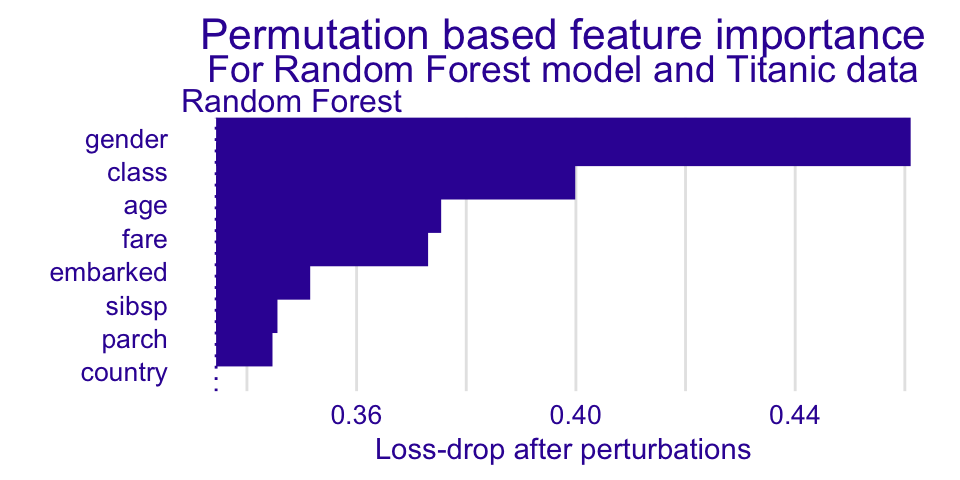
\includegraphics{PM_VEE_files/figure-latex/titanic3-1.pdf}
\caption{\label{fig:titanic3}Feature importance. Each interval presents the
difference between original model performance (left end) and the
performance on a dataset with a single feature perturbed}
\end{figure}

It's interesting that the most important variable for Titanic data is
the Sex. So it have been ,,women first'' after all. Then the three
features of similar importance are passenger class (first class has
higher survival), age (kids have higher survival) and fare (owners of
more pricy tickets have higher survival).

Note that drawing permutations evolves some randomness. Thus to have
higher repeatability of results you may either set a seed for random
number generator or replicate the procedure few times. The second
approach has additional advantage, that you will learn the uncertainty
behind feature importance assessment.

Here we present scores for 10 repetition of the process.

\begin{Shaded}
\begin{Highlighting}[]
\NormalTok{fi_rf10 <-}\StringTok{ }\KeywordTok{replicate}\NormalTok{(}\DecValTok{10}\NormalTok{, }\KeywordTok{feature_importance}\NormalTok{(explainer_rf), }\DataTypeTok{simplify =} \OtherTok{FALSE}\NormalTok{)}
\KeywordTok{do.call}\NormalTok{(plot, fi_rf10) }\OperatorTok{+}\StringTok{ }\KeywordTok{ggtitle}\NormalTok{(}\StringTok{"Permutation based feature importance"}\NormalTok{, }\StringTok{"For Random Forest model and Titanic data"}\NormalTok{)}
\end{Highlighting}
\end{Shaded}

\begin{figure}
\centering
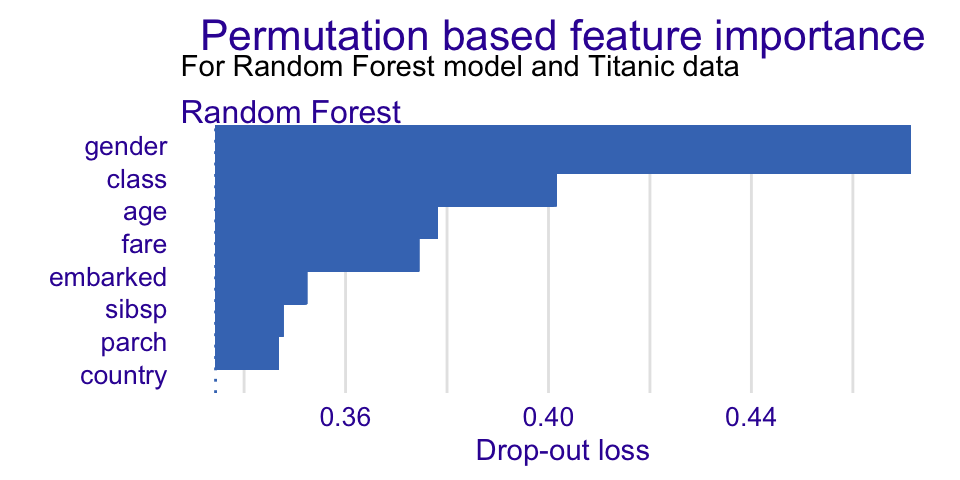
\includegraphics{PM_VEE_files/figure-latex/titanic4-1.pdf}
\caption{\label{fig:titanic4}Feature importance for 10 replication of
feature importance assessment}
\end{figure}

It is much easier to assess feature importance if they come with some
assessment of the uncertainty. We can read from the plot that Age and
passenger class are close to each other.

Note that intervals are useful for model comparisons. In the Figure
@ref\{titanic5\} we can read feature importance for random forest,
gradient boosting and logistic regression models. Best results are
achieved by the random forest model and also this method consume more
features than others. A good example is the \emph{Fare} variable, not
used in gradient boosting not logistic regression (as a feature highly
correlated with passenger class) but consumed in the random forest
model.

\begin{Shaded}
\begin{Highlighting}[]
\NormalTok{fi_rf <-}\StringTok{ }\KeywordTok{feature_importance}\NormalTok{(explainer_rf)}
\NormalTok{fi_gbm <-}\StringTok{ }\KeywordTok{feature_importance}\NormalTok{(explainer_gbm)}
\NormalTok{fi_glm <-}\StringTok{ }\KeywordTok{feature_importance}\NormalTok{(explainer_glm)}

\KeywordTok{plot}\NormalTok{(fi_rf, fi_gbm, fi_glm)}
\end{Highlighting}
\end{Shaded}

\begin{figure}
\centering
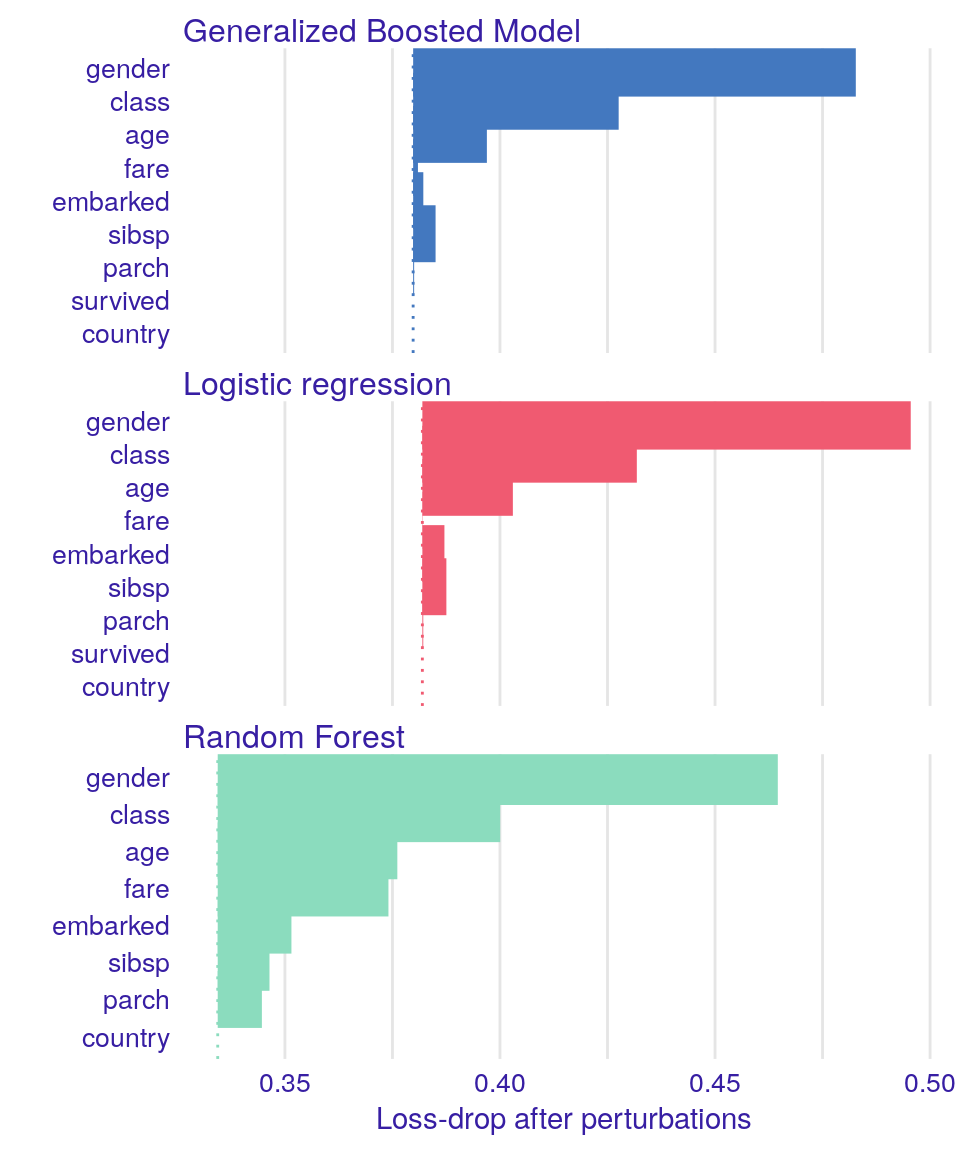
\includegraphics{PM_VEE_files/figure-latex/titanic5-1.pdf}
\caption{\label{fig:titanic5}Feature importance for random forest, gradient
boosting and logistic regression models}
\end{figure}

\hypertarget{example-price-prediction}{%
\subsection{Example: Price prediction}\label{example-price-prediction}}

Let's create a regression model for prediction of apartment prices.

\begin{Shaded}
\begin{Highlighting}[]
\KeywordTok{library}\NormalTok{(}\StringTok{"DALEX"}\NormalTok{)}
\KeywordTok{library}\NormalTok{(}\StringTok{"randomForest"}\NormalTok{)}
\KeywordTok{set.seed}\NormalTok{(}\DecValTok{59}\NormalTok{)}
\NormalTok{model_rf <-}\StringTok{ }\KeywordTok{randomForest}\NormalTok{(m2.price }\OperatorTok{~}\StringTok{ }\NormalTok{construction.year }\OperatorTok{+}\StringTok{ }\NormalTok{surface }\OperatorTok{+}\StringTok{ }\NormalTok{floor }\OperatorTok{+}\StringTok{ }
\StringTok{                           }\NormalTok{no.rooms }\OperatorTok{+}\StringTok{ }\NormalTok{district, }\DataTypeTok{data =}\NormalTok{ apartments)}
\end{Highlighting}
\end{Shaded}

A popular loss function for regression model is the root mean square
loss \[
  L(x, y) = \sqrt{\frac1n \sum_{i=1}^n (x_i - y_i)^2}
\]

\begin{Shaded}
\begin{Highlighting}[]
\KeywordTok{loss_root_mean_square}\NormalTok{(}
  \KeywordTok{predict}\NormalTok{(model_rf, apartments), }
\NormalTok{  apartments}\OperatorTok{$}\NormalTok{m2.price}
\NormalTok{)}
\end{Highlighting}
\end{Shaded}

\begin{verbatim}
## [1] 193.8477
\end{verbatim}

Let's calculate feature importance

\begin{Shaded}
\begin{Highlighting}[]
\NormalTok{explainer_rf <-}\StringTok{ }\KeywordTok{explain}\NormalTok{(model_rf, }
            \DataTypeTok{data =}\NormalTok{ apartmentsTest[,}\DecValTok{2}\OperatorTok{:}\DecValTok{6}\NormalTok{], }\DataTypeTok{y =}\NormalTok{ apartmentsTest}\OperatorTok{$}\NormalTok{m2.price)}
\NormalTok{vip <-}\StringTok{ }\KeywordTok{variable_importance}\NormalTok{(explainer_rf, }
            \DataTypeTok{loss_function =}\NormalTok{ loss_root_mean_square)}
\NormalTok{vip}
\end{Highlighting}
\end{Shaded}

\begin{verbatim}
##            variable dropout_loss        label
## 1      _full_model_     285.1355 randomForest
## 2          no.rooms     391.0710 randomForest
## 3 construction.year     410.5866 randomForest
## 4             floor     445.2164 randomForest
## 5           surface     480.1431 randomForest
## 6          district     843.6519 randomForest
## 7        _baseline_    1081.3710 randomForest
\end{verbatim}

On a diagnostic plot is useful to present feature importance as an
interval that start in a loss and ends in a loss of perturbed data.

\begin{Shaded}
\begin{Highlighting}[]
\KeywordTok{plot}\NormalTok{(vip)}
\end{Highlighting}
\end{Shaded}

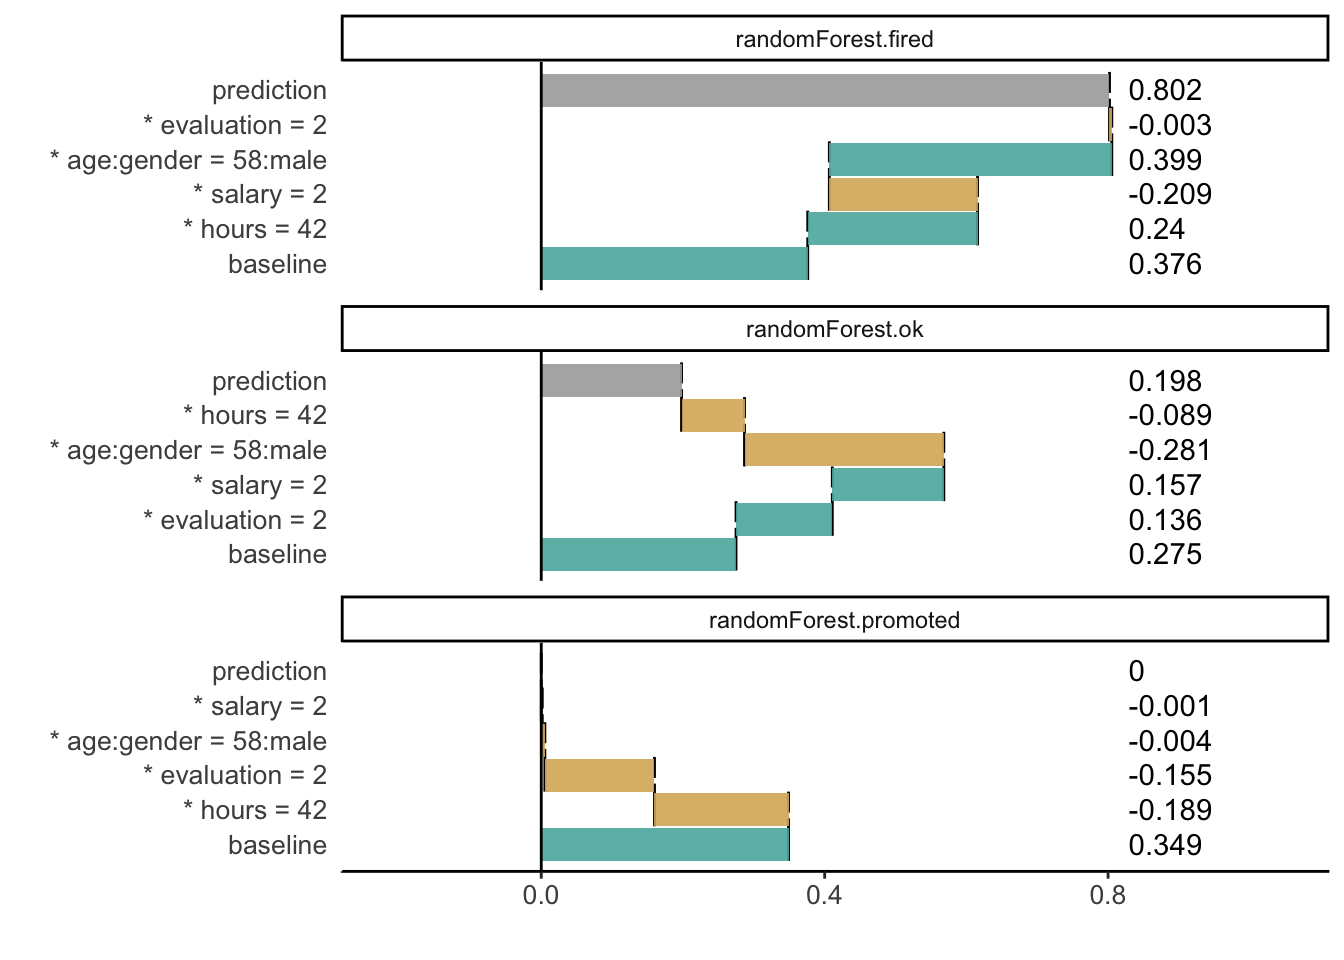
\includegraphics{PM_VEE_files/figure-latex/unnamed-chunk-43-1.pdf}

\hypertarget{more-models}{%
\subsection{More models}\label{more-models}}

Much more can be read from feature importance plots if we compare models
of a different structure. Let's train three predictive models trained on
\texttt{apartments} dataset from the \texttt{DALEX} package. Random
Forest model \citep{R-randomForest} (elastic but biased), Support Vector
Machines model \citep{R-e1071} (large variance on boundaries) and Linear
Model (stable but not very elastic). Presented examples are for
regression (prediction of square meter price), but the CP profiles may
be used in the same way for classification.

Let's fit these three models.

\begin{Shaded}
\begin{Highlighting}[]
\KeywordTok{library}\NormalTok{(}\StringTok{"DALEX"}\NormalTok{)}
\NormalTok{model_lm <-}\StringTok{ }\KeywordTok{lm}\NormalTok{(m2.price }\OperatorTok{~}\StringTok{ }\NormalTok{construction.year }\OperatorTok{+}\StringTok{ }\NormalTok{surface }\OperatorTok{+}\StringTok{ }\NormalTok{floor }\OperatorTok{+}\StringTok{ }
\StringTok{                      }\NormalTok{no.rooms }\OperatorTok{+}\StringTok{ }\NormalTok{district, }\DataTypeTok{data =}\NormalTok{ apartments)}

\KeywordTok{library}\NormalTok{(}\StringTok{"randomForest"}\NormalTok{)}
\KeywordTok{set.seed}\NormalTok{(}\DecValTok{59}\NormalTok{)}
\NormalTok{model_rf <-}\StringTok{ }\KeywordTok{randomForest}\NormalTok{(m2.price }\OperatorTok{~}\StringTok{ }\NormalTok{construction.year }\OperatorTok{+}\StringTok{ }\NormalTok{surface }\OperatorTok{+}\StringTok{ }\NormalTok{floor }\OperatorTok{+}\StringTok{ }
\StringTok{                      }\NormalTok{no.rooms }\OperatorTok{+}\StringTok{ }\NormalTok{district, }\DataTypeTok{data =}\NormalTok{ apartments)}

\KeywordTok{library}\NormalTok{(}\StringTok{"e1071"}\NormalTok{)}
\NormalTok{model_svm <-}\StringTok{ }\KeywordTok{svm}\NormalTok{(m2.price }\OperatorTok{~}\StringTok{ }\NormalTok{construction.year }\OperatorTok{+}\StringTok{ }\NormalTok{surface }\OperatorTok{+}\StringTok{ }\NormalTok{floor }\OperatorTok{+}\StringTok{ }
\StringTok{                         }\NormalTok{no.rooms }\OperatorTok{+}\StringTok{ }\NormalTok{district, }\DataTypeTok{data =}\NormalTok{ apartments)}
\end{Highlighting}
\end{Shaded}

For these models we use \texttt{DALEX} explainers created with
\texttt{explain()} function. These explainers wrap models, predict
functions and validation data.

\begin{Shaded}
\begin{Highlighting}[]
\NormalTok{explainer_lm <-}\StringTok{ }\KeywordTok{explain}\NormalTok{(model_lm, }
                       \DataTypeTok{data =}\NormalTok{ apartmentsTest[,}\DecValTok{2}\OperatorTok{:}\DecValTok{6}\NormalTok{], }\DataTypeTok{y =}\NormalTok{ apartmentsTest}\OperatorTok{$}\NormalTok{m2.price)}
\NormalTok{vip_lm <-}\StringTok{ }\KeywordTok{variable_importance}\NormalTok{(explainer_lm, }
            \DataTypeTok{loss_function =}\NormalTok{ loss_root_mean_square)}
\NormalTok{vip_lm}
\end{Highlighting}
\end{Shaded}

\begin{verbatim}
##            variable dropout_loss label
## 1      _full_model_     282.0062    lm
## 2 construction.year     281.9007    lm
## 3          no.rooms     292.8398    lm
## 4             floor     492.0857    lm
## 5           surface     614.9198    lm
## 6          district    1002.3487    lm
## 7        _baseline_    1193.6209    lm
\end{verbatim}

\begin{Shaded}
\begin{Highlighting}[]
\NormalTok{explainer_rf <-}\StringTok{ }\KeywordTok{explain}\NormalTok{(model_rf, }
                       \DataTypeTok{data =}\NormalTok{ apartmentsTest[,}\DecValTok{2}\OperatorTok{:}\DecValTok{6}\NormalTok{], }\DataTypeTok{y =}\NormalTok{ apartmentsTest}\OperatorTok{$}\NormalTok{m2.price)}
\NormalTok{vip_rf <-}\StringTok{ }\KeywordTok{variable_importance}\NormalTok{(explainer_rf, }
            \DataTypeTok{loss_function =}\NormalTok{ loss_root_mean_square)}
\NormalTok{vip_rf}
\end{Highlighting}
\end{Shaded}

\begin{verbatim}
##            variable dropout_loss        label
## 1      _full_model_     293.2729 randomForest
## 2          no.rooms     389.4526 randomForest
## 3 construction.year     416.1154 randomForest
## 4             floor     453.9195 randomForest
## 5           surface     480.4062 randomForest
## 6          district     867.7050 randomForest
## 7        _baseline_    1116.2616 randomForest
\end{verbatim}

\begin{Shaded}
\begin{Highlighting}[]
\NormalTok{explainer_svm <-}\StringTok{ }\KeywordTok{explain}\NormalTok{(model_svm, }
                       \DataTypeTok{data =}\NormalTok{ apartmentsTest[,}\DecValTok{2}\OperatorTok{:}\DecValTok{6}\NormalTok{], }\DataTypeTok{y =}\NormalTok{ apartmentsTest}\OperatorTok{$}\NormalTok{m2.price)}
\NormalTok{vip_svm <-}\StringTok{ }\KeywordTok{variable_importance}\NormalTok{(explainer_svm, }
            \DataTypeTok{loss_function =}\NormalTok{ loss_root_mean_square)}
\NormalTok{vip_svm}
\end{Highlighting}
\end{Shaded}

\begin{verbatim}
##            variable dropout_loss label
## 1      _full_model_     157.7938   svm
## 2          no.rooms     221.4595   svm
## 3 construction.year     365.2600   svm
## 4             floor     439.8724   svm
## 5           surface     527.2598   svm
## 6          district     942.8512   svm
## 7        _baseline_    1203.7571   svm
\end{verbatim}

Let's plot feature importance for all three models on a single plot.

Intervals start in a different values, thus we can read that loss for
SVM model is the lowest.

When we compare other features it looks like in all models the
\texttt{district} is the most important feature followed by
\texttt{surface} and \texttt{floor}.

\begin{Shaded}
\begin{Highlighting}[]
\KeywordTok{plot}\NormalTok{(vip_rf, vip_svm, vip_lm)}
\end{Highlighting}
\end{Shaded}

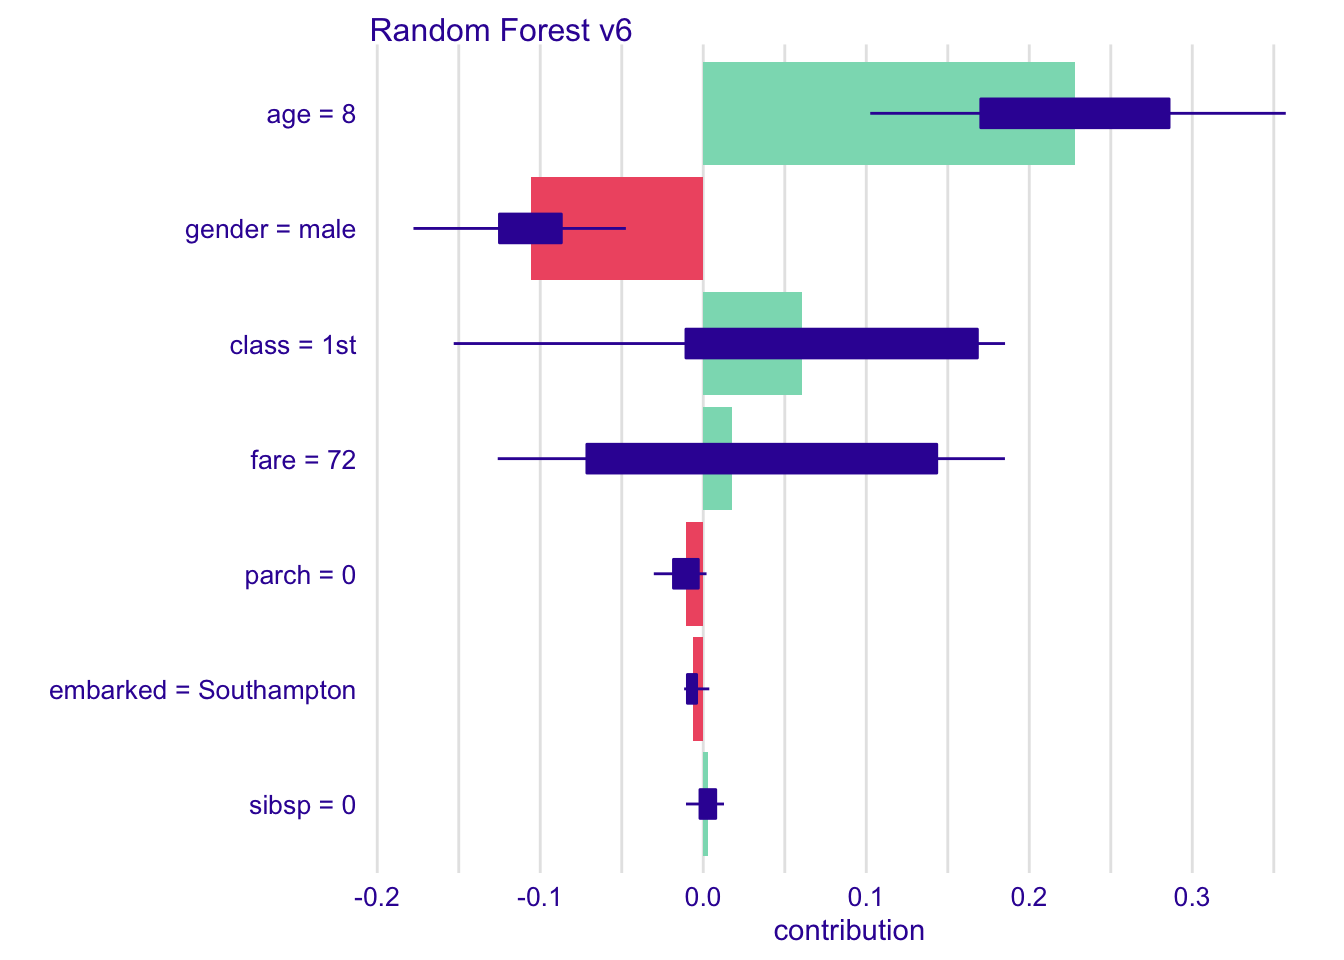
\includegraphics{PM_VEE_files/figure-latex/unnamed-chunk-46-1.pdf}

There is interesting difference between linear model and others in the
way how important is the \texttt{construction.year}. For linear model
this variable is not importance, while for remaining two models there is
some importance.

In the next chapter we will see how this is possible.

\hypertarget{level-frequency}{%
\subsection{Level frequency}\label{level-frequency}}

What does the feature importance mean? How it is linked with a data
distribution.

\hypertarget{variableEngeneering}{%
\section{Feature effects}\label{variableEngeneering}}

Methods presented in this chapter are useful for extraction information
of feature effect, i.e.~how a feature is linked with model response.
There are many possible applications of such methods, for example:

\begin{itemize}
\tightlist
\item
  Feature effect may be used for feature engineering. Surrogate training
  is a procedure in which an elastic model is trained to learn about
  link between a feature and the target. Then a new feature is created
  in a way to better utilized the feature in a simpler model.
\item
  Understanding how the model utilize a feature may be used as a
  validation of a model against domain knowledge. For example if we
  expect monotonic relation or linear relation then such assumptions may
  be testes
\item
  Understanding of a link between target and the feature may increase
  our domain knowledge.
\item
  Comparison of feature effects between different models may help us to
  understand how different models handle particular features.
\end{itemize}

\begin{verbatim}
## Distribution not specified, assuming bernoulli ...
\end{verbatim}

\hypertarget{partialDependence}{%
\subsection{Partial Dependency Plots}\label{partialDependence}}

One of the first and the most popular tools for model understanding are
Partial Dependence Plots (sometimes named Partial Dependence Profiles)
\citep{Friedman00greedyfunction}.

PDP was introduced by Friedman in 2000 in the paper devoted to Gradient
Boosting Machines (GBM) - new type of complex yet effective models. For
many years PDP as sleeping beauties stay in the shadow of the boosting.
It has changed in recent years.

General idea is to show how the expected model response behaves as a
function of a selected feature. Here the word ,,expected'' means
averaged over the population. We can think about them as about an
average from Ceteris Paribus Profiles introduced in
@ref\{ceterisParibus\}.

Let's see how they are constructed step by step. Here we will use a
\emph{random forest model} created for the \emph{titanic} dataset.
Examples are related to a single variable \emph{Age}.

\begin{enumerate}
\def\labelenumi{\arabic{enumi}.}
\tightlist
\item
  Calculate Ceteris Paribus profiles for observations from the dataset
\end{enumerate}

As it was introduced in @ref\{ceterisParibus\} Ceteris Paribus profiles
are calculated for observations. They show how model response change is
a selected variable in this observation is modified.

\[
CP^{f, j, x}(z) := f(x|^j = z).
\]

Such profiles can be calculated for example with the
\texttt{ceteris\_paribus\{ingredients\}} function.

\begin{Shaded}
\begin{Highlighting}[]
\KeywordTok{library}\NormalTok{(}\StringTok{"ingredients"}\NormalTok{)}
\NormalTok{selected_passangers <-}\StringTok{ }\KeywordTok{select_sample}\NormalTok{(titanic_small, }\DataTypeTok{n =} \DecValTok{100}\NormalTok{)}
\NormalTok{cp_rf <-}\StringTok{ }\KeywordTok{ceteris_paribus}\NormalTok{(explainer_rf, selected_passangers)}
\end{Highlighting}
\end{Shaded}

So for a single model and a single variable we get a bunch of
\emph{what-if} profiles. In the figure @ref\{pdp\_part\_1\} we show an
example for 100 observations. Despite some variation (random forest are
not as stable as we would hope) we see that most profiles are
decreasing. So the older the passengers is the lower is the survival
probability.

\begin{figure}
\centering
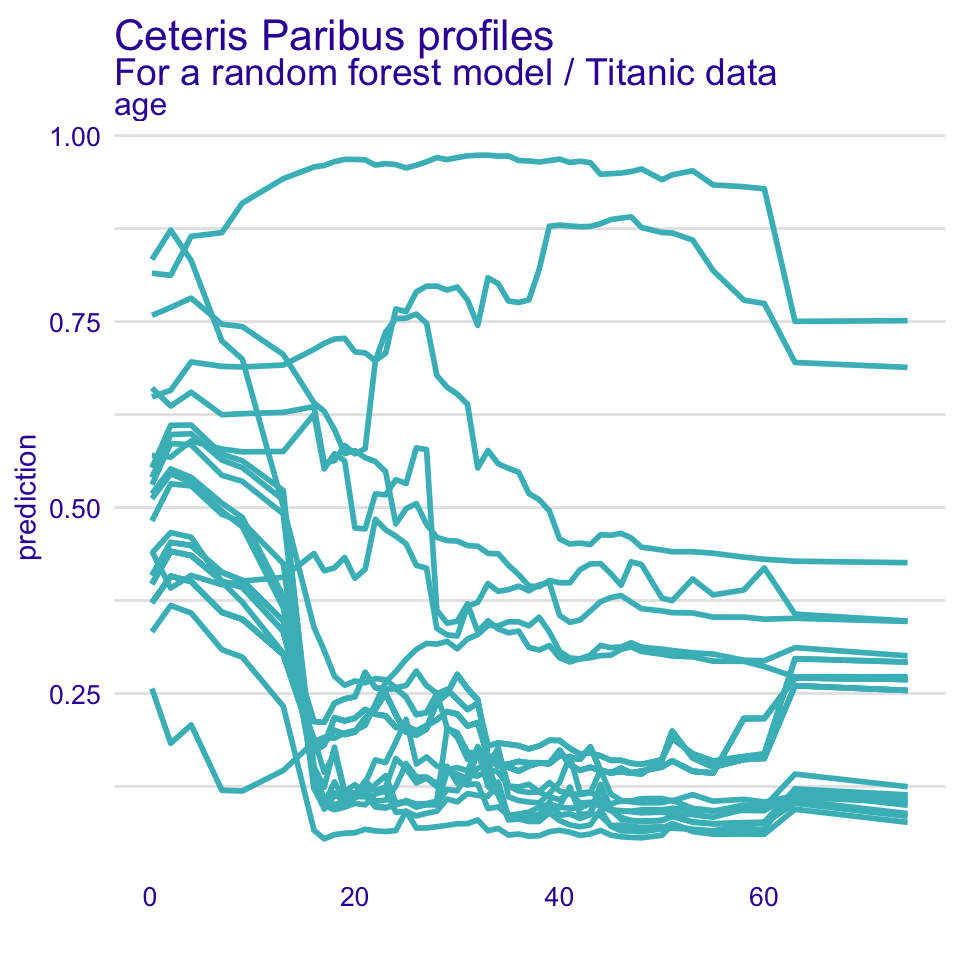
\includegraphics{PM_VEE_files/figure-latex/pdp_part_1-1.pdf}
\caption{(\#fig:pdp\_part\_1)Ceteris Paribus profiles for 100
observations, the Age variable and the random forest model}
\end{figure}

\begin{enumerate}
\def\labelenumi{\arabic{enumi}.}
\setcounter{enumi}{1}
\tightlist
\item
  Aggregate Ceteris Paribus into a single Partial Dependency Profile
\end{enumerate}

In the most common formulation Partial Dependency Plots are expected
values for CP profiles (see \texttt{pdp} package \citep{pdp}).

\[
g_i(z) = E_{x_{-i}}[ f(x|^i = z, x^{-i}) ].
\]

Of course, this expectation cannot be calculated directly as we do not
know fully neither the distribution of \(x_{-i}\) nor the \(f()\). Yet
this value may be estimated by

\[
\hat g_i(z) = \frac{1}{n} \sum_{j=1}^{n} f(x|^i = z, x_j^{-i}).
\]

Such average can be calculated with the
\texttt{aggregate\_profiles\{ingredients\}} function.

\begin{Shaded}
\begin{Highlighting}[]
\KeywordTok{library}\NormalTok{(}\StringTok{"ingredients"}\NormalTok{)}
\NormalTok{selected_passangers <-}\StringTok{ }\KeywordTok{select_sample}\NormalTok{(titanic_small, }\DataTypeTok{n =} \DecValTok{100}\NormalTok{)}
\NormalTok{cp_rf <-}\StringTok{ }\KeywordTok{ceteris_paribus}\NormalTok{(explainer_rf, selected_passangers)}
\NormalTok{pdp_rf <-}\StringTok{ }\KeywordTok{aggregate_profiles}\NormalTok{(cp_rf, }\DataTypeTok{selected_variables =} \StringTok{"Age"}\NormalTok{)}
\end{Highlighting}
\end{Shaded}

So for a single model and a single variable we get a profile. See an
example in figure @ref\{pdp\_part\_2\}. It is much easier than following
100 separate curves, and in cases in which Ceteris Paribus are more or
less parallel, the Partial Dependency is a good summary of them.

The average response is of course more stable (as it's an average) and
in this case is more or less a decreasing curve. It's much easier to
notice that the older the passenger is the lower the survival
probability. Moreover it is easier to notice that the largest drop in
survival changes happen for teenagers. On average the survival for
adults is 30 percent points smaller than for kids.

\begin{figure}
\centering
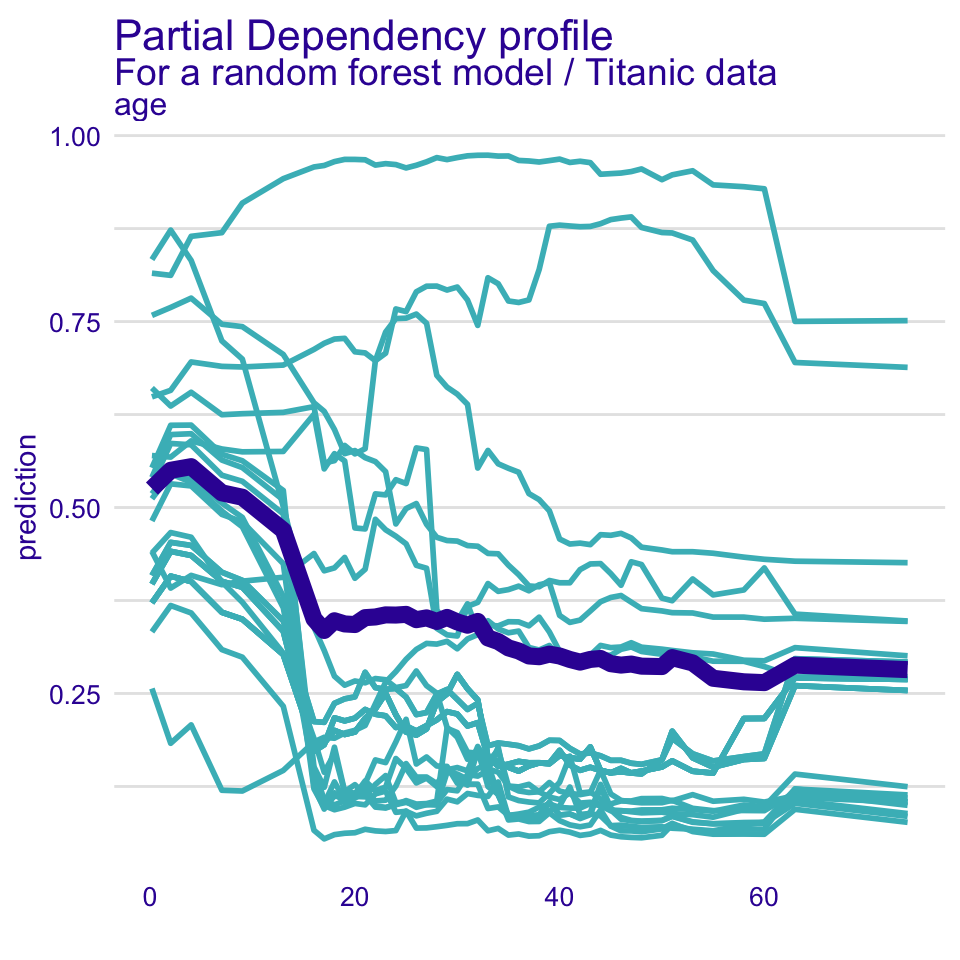
\includegraphics{PM_VEE_files/figure-latex/pdp_part_2-1.pdf}
\caption{(\#fig:pdp\_part\_2)Partial Dependency profile as an average
for 100 observations}
\end{figure}

\hypertarget{interactions-and-partial-dependency-profiles}{%
\subsubsection{Interactions and Partial Dependency
profiles}\label{interactions-and-partial-dependency-profiles}}

As we said in the previous section, Partial Dependency is a good summary
if Ceteris Paribus profiles are similar, i.e.~parallel. But it may
happen that the variable of interest is in interaction with some other
variable. Then profiles are not parallel because the effect of variable
of interest depends on some other variables.

So on one hand it would be good to summaries all this Ceteris Paribus
profiles with smaller number of profiles. But on another hand a single
aggregate may not be enough. To deal with this problem we propose to
cluster Ceteris Paribus profiles and check how homogenous are these
profiles.

The most straightforward approach would be to use a method for
clustering, like k-means algorithm or hierarchical clustering, and see
how these cluster of profiles behave. Once clusters are established we
can aggregate within clusters in the same way as in case of Partial
Dependency Plots.

Such clusters can be calculated with the
\texttt{cluster\_profiles\{ingredients\}} function. We choose the
hierarchical clustering with Ward linkage as it gives most stable
results.

\begin{Shaded}
\begin{Highlighting}[]
\KeywordTok{library}\NormalTok{(}\StringTok{"ingredients"}\NormalTok{)}
\NormalTok{selected_passangers <-}\StringTok{ }\KeywordTok{select_sample}\NormalTok{(titanic_small, }\DataTypeTok{n =} \DecValTok{100}\NormalTok{)}
\NormalTok{cp_rf <-}\StringTok{ }\KeywordTok{ceteris_paribus}\NormalTok{(explainer_rf, selected_passangers)}
\NormalTok{clust_rf <-}\StringTok{ }\KeywordTok{cluster_profiles}\NormalTok{(cp_rf, }\DataTypeTok{k =} \DecValTok{3}\NormalTok{, }\DataTypeTok{selected_variables =} \StringTok{"Age"}\NormalTok{)}
\end{Highlighting}
\end{Shaded}

So for a single model and a single variable we get \(k\) profiles. The
common problem in clustering is the selection of \(k\). However in our
case, as it's an exploration, the problem is simpler, as we are
interesting if \(k=1\) (Partial Dependency is a good summary) or not
(there are some interactions).

See an example in Figure @ref\{pdp\_part\_4\}. It is easier to notice
that Ceteris Paribus profiles can be groups in three clusters. Group of
passengers with a very large drop in the survival (cluster 1), moderate
drop (cluster 2) and almost no drop in survival (cluster 3). Here we do
not know what other factors are linked with these clusters, but some
additional exploratory analysis can be done to identify these factors.

\begin{figure}
\centering
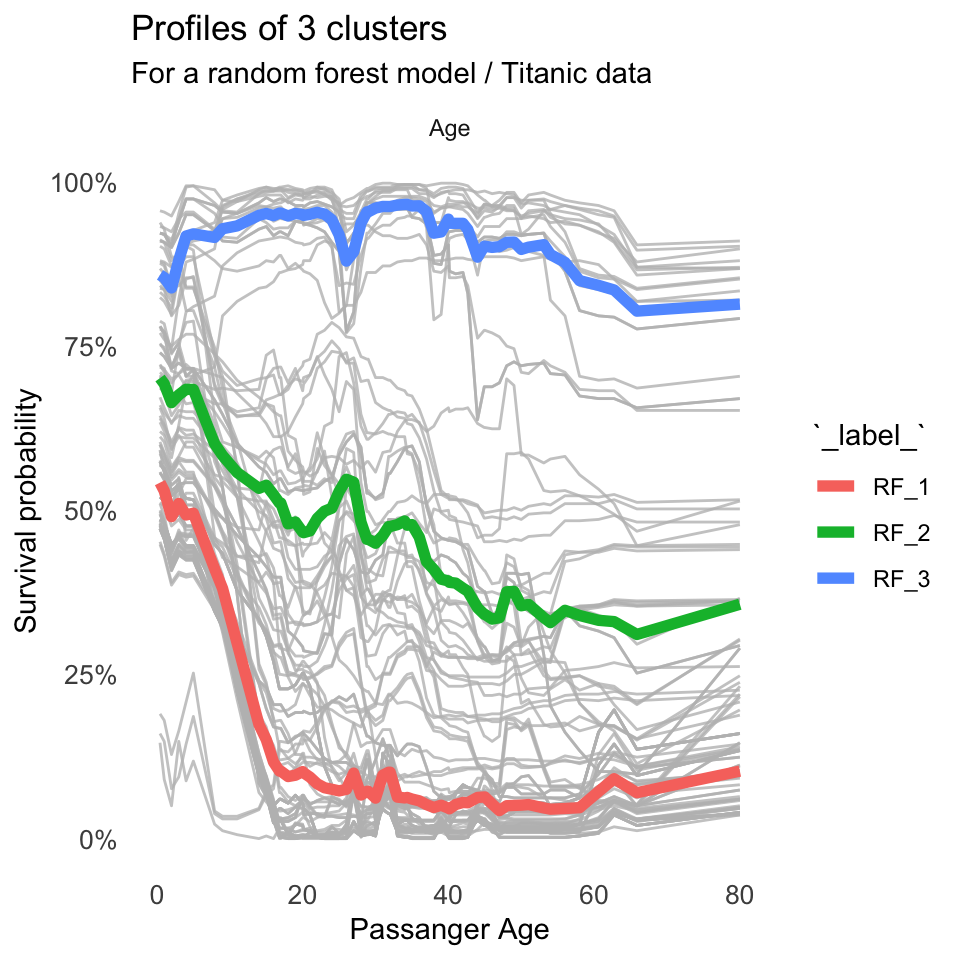
\includegraphics{PM_VEE_files/figure-latex/pdp_part_4-1.pdf}
\caption{(\#fig:pdp\_part\_4)Cluster profiles for 3 clusters over 100
Ceteris Paribus profiles}
\end{figure}

\hypertarget{groups-of-partial-dependency-profiles}{%
\subsubsection{Groups of Partial Dependency
profiles}\label{groups-of-partial-dependency-profiles}}

Once we see that variable of interest may be in interaction with some
other variable, it is tempting to look for the factor that distinguish
clusters.

The most straightforward approach is to use some other variable as a
grouping variable. This can be done by setting the \texttt{groups}
argument in the \texttt{aggregate\_profiles\{ingredients\}} function.

\begin{Shaded}
\begin{Highlighting}[]
\KeywordTok{library}\NormalTok{(}\StringTok{"ingredients"}\NormalTok{)}
\NormalTok{selected_passangers <-}\StringTok{ }\KeywordTok{select_sample}\NormalTok{(titanic_small, }\DataTypeTok{n =} \DecValTok{100}\NormalTok{)}
\NormalTok{cp_rf <-}\StringTok{ }\KeywordTok{ceteris_paribus}\NormalTok{(explainer_rf, selected_passangers)}
\NormalTok{pdp_Sex_rf <-}\StringTok{ }\KeywordTok{aggregate_profiles}\NormalTok{(cp_rf, }\DataTypeTok{selected_variables =} \StringTok{"Age"}\NormalTok{,}
                \DataTypeTok{groups =} \StringTok{"Sex"}\NormalTok{)}
\end{Highlighting}
\end{Shaded}

See an example in Figure @ref\{pdp\_part\_5\}. Clearly there is an
interaction between Age and Sex. The survival for woman is more stable,
while for man there is more sudden drop in Survival for older
passengers. Check how the interaction for \texttt{Pclass} (passenger
class) looks like.

\begin{figure}
\centering
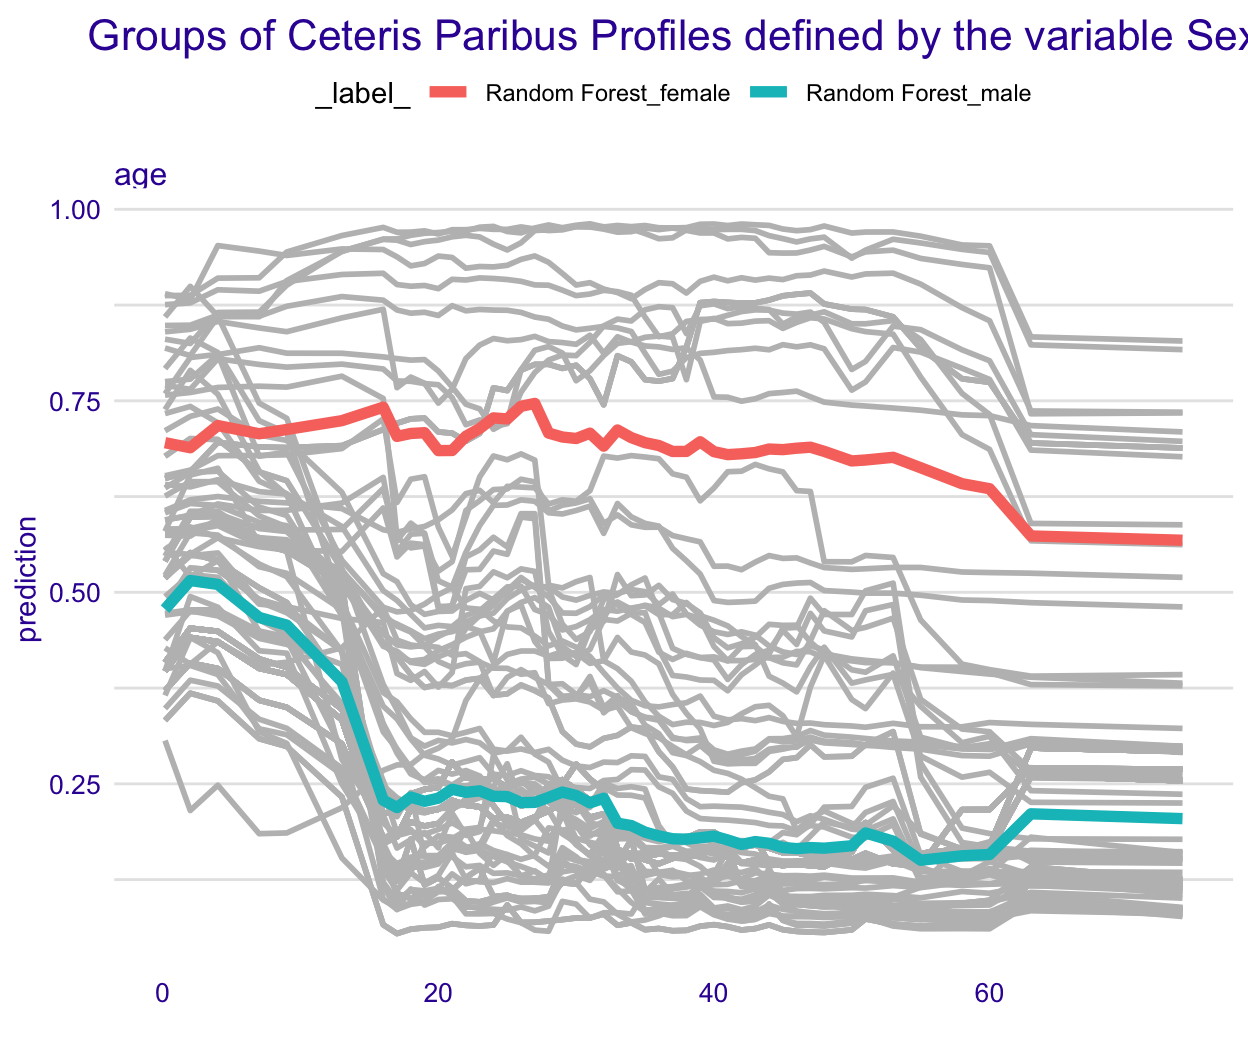
\includegraphics{PM_VEE_files/figure-latex/pdp_part_5-1.pdf}
\caption{(\#fig:pdp\_part\_5)Grouped profiles with respect to the Sex
variable}
\end{figure}

\hypertarget{model-comparisons-with-partial-dependency-plots}{%
\subsubsection{Model comparisons with Partial Dependency
Plots}\label{model-comparisons-with-partial-dependency-plots}}

Contrastive comparisons of Partial Dependency Plots are useful not only
for subgroups of observations but also for model comparisons.

Why one would like to compare models? There are at least three reasons
for it.

\begin{itemize}
\tightlist
\item
  \emph{Agreement of models will calm us.} Some models are known to be
  more stable other to be more elastic. If profiles for models from
  these two classes are not far from each other we can be more convinced
  that elastic model is not over-fitted.
\item
  \emph{Disagreement of models helps to improve.} If simpler
  interpretable model disagree with an elastic model, this may suggest a
  feature transformation that can be used to improve the interpretable
  model. For example if random forest learned non linear relation then
  it can be captures by a linear model after suitable transformation.
\item
  \emph{Validation of boundary conditions.} Some models are know to have
  different behavior on the boundary, for largest or lowest values.
  Random forest is known to shrink predictions towards the average,
  while support vector machines are known to have larger variance at
  edges. Contrastive comparisons may help to understand differences in
  boundary behavior.
\end{itemize}

Generic \texttt{plot\{ingredients\}} function handles multiple models as
consecutive arguments.

\begin{Shaded}
\begin{Highlighting}[]
\KeywordTok{library}\NormalTok{(}\StringTok{"ingredients"}\NormalTok{)}
\KeywordTok{plot}\NormalTok{(pdp_rf, pdp_glm, pdp_gbm, }\DataTypeTok{selected_variables =} \StringTok{"Age"}\NormalTok{, }\DataTypeTok{color =} \StringTok{"_label_"}\NormalTok{)}
\end{Highlighting}
\end{Shaded}

See an example in Figure @ref\{pdp\_part\_7\}. Random forest is compared
with gradient boosting model and generalized linear model (logistic
regression). All three models agree when it comes to a general relation
between Age and Survival. Logistic regression is of course the most
smooth. Gradient boosting has on average higher predictions than random
forest.

\begin{figure}
\centering
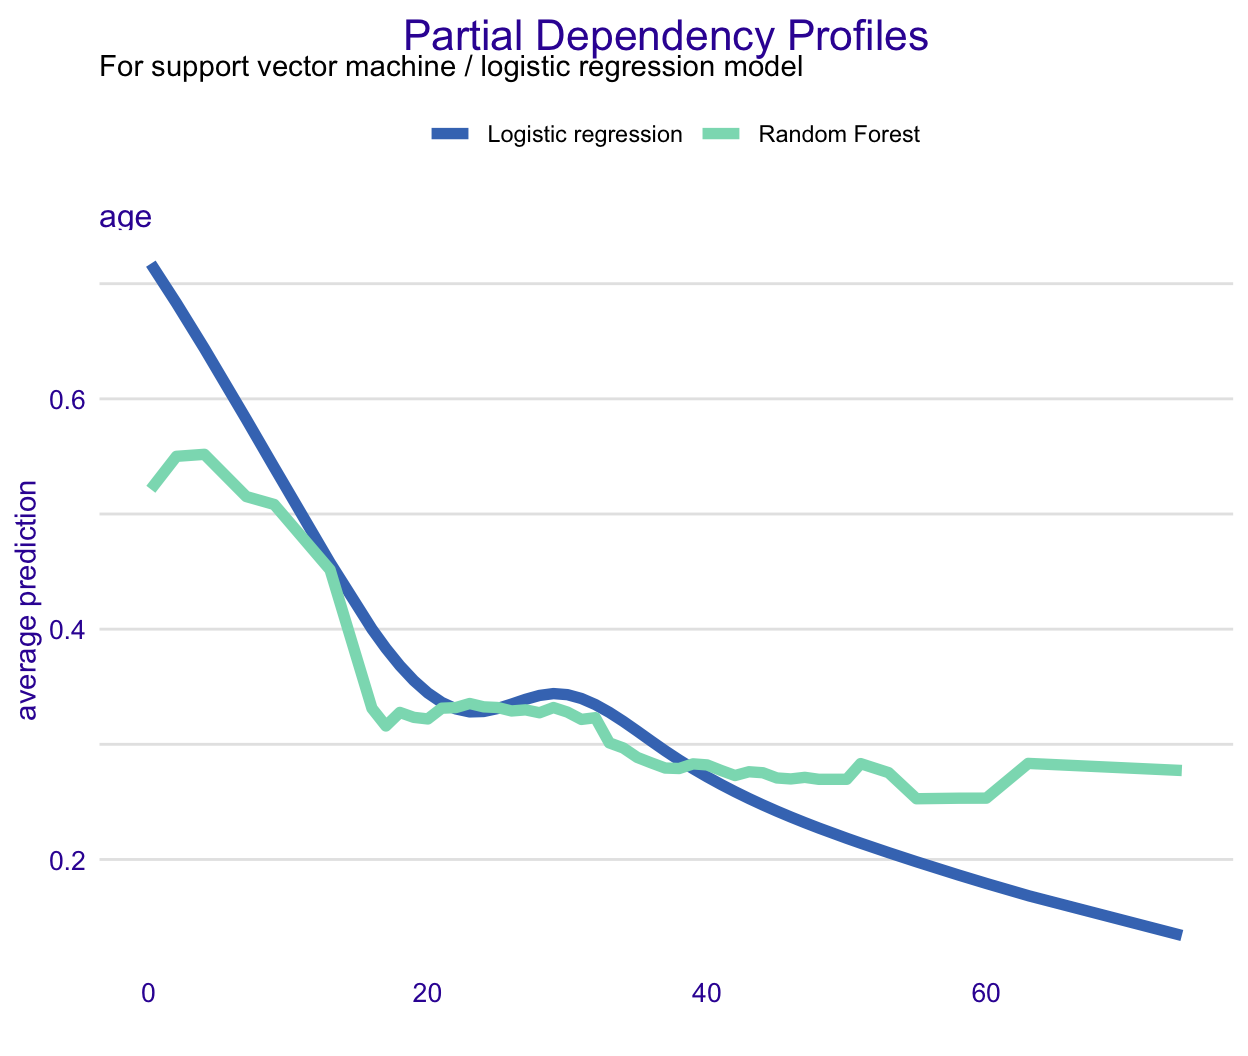
\includegraphics{PM_VEE_files/figure-latex/pdp_part_7-1.pdf}
\caption{(\#fig:pdp\_part\_7)Comparison on three predictive models with
different structures.}
\end{figure}

\hypertarget{correlation-between-features}{%
\subsubsection{Correlation between
features}\label{correlation-between-features}}

One of the largest advantages of the Partial Dependency Profiles is that
they are easy to explain, as they are just an average across Ceteris
Paribus profiles. But one of the largest disadvantages lies in
assumptions of CPs. Profiles are created based on assumption that it
makes sense to change variable \(x^i\) independently from all other
variables \(x^{-i}\).

But this may not have sense at all. Features like \(surface\) and
\(number.or.rooms\) are strongly correlated as apartments with larger
number of rooms usually have larger surface. It may makes no sense to
consider an apartment with 10 rooms and 20 square meters, so it may be
misleading to change \(x^{surface}\) independently from
\(x^{number.of.rooms}\).

There are several attempts to fix this problem. One of the most known
are Accumulated Local Effects Plots (ALEPlots) \citep{R-ALEPlot} or
Local Conditional Expectation Profiles (LCE) {[}TODO: referencja do
pracy Rafala{]}?

\hypertarget{merging-path-plots}{%
\subsection{Merging Path Plots}\label{merging-path-plots}}

\citep{demsar2018}

\citep{RJ2017016} \citep{MAGIX}

\citep{R-factorMerger}

\citep{Strobl2007} \citep{Strobl2008} - variable importance

\citep{2018arXiv180101489F}

Beware Default Random Forest Importances

Terence Parr, Kerem Turgutlu, Christopher Csiszar, and Jeremy Howard
March 26, 2018.

\url{http://explained.ai/rf-importance/index.html}

\citep{R-factorMerger}

\begin{Shaded}
\begin{Highlighting}[]
\KeywordTok{library}\NormalTok{(factorMerger)}
\end{Highlighting}
\end{Shaded}

\hypertarget{other-topics}{%
\section{Other topics}\label{other-topics}}

\citep{R-randomForestExplainer} \citep{R-ICEbox} \citep{R-ALEPlot}

\citep{R-modelDown}

\hypertarget{modelComparisons}{%
\section{Performance Diagnostic}\label{modelComparisons}}

Goal: how good is the model, which is better

Model selection

\begin{itemize}
\tightlist
\item
  ROC / RROC / LIFT
\end{itemize}

\begin{Shaded}
\begin{Highlighting}[]
\KeywordTok{library}\NormalTok{(}\StringTok{"auditor"}\NormalTok{)}
\KeywordTok{library}\NormalTok{(}\StringTok{"DALEX2"}\NormalTok{)}
\KeywordTok{library}\NormalTok{(}\StringTok{"ranger"}\NormalTok{)}
\KeywordTok{library}\NormalTok{(}\StringTok{"e1071"}\NormalTok{)}

\NormalTok{rf_model <-}\StringTok{ }\KeywordTok{ranger}\NormalTok{(life_length }\OperatorTok{~}\StringTok{ }\NormalTok{., }\DataTypeTok{data =}\NormalTok{ dragons)}
\NormalTok{lm_model <-}\StringTok{ }\KeywordTok{lm}\NormalTok{(life_length }\OperatorTok{~}\StringTok{ }\NormalTok{., }\DataTypeTok{data =}\NormalTok{ dragons)}
\NormalTok{svm_model <-}\StringTok{ }\KeywordTok{svm}\NormalTok{(life_length }\OperatorTok{~}\StringTok{ }\NormalTok{., }\DataTypeTok{data =}\NormalTok{ dragons)}

\NormalTok{predict_function <-}\StringTok{ }\ControlFlowTok{function}\NormalTok{(m,x,...) }\KeywordTok{predict}\NormalTok{(m, x, ...)}\OperatorTok{$}\NormalTok{predictions}
\NormalTok{rf_au <-}\StringTok{ }\KeywordTok{audit}\NormalTok{(rf_model, }\DataTypeTok{data =}\NormalTok{ dragons, }\DataTypeTok{y =}\NormalTok{ dragons}\OperatorTok{$}\NormalTok{life_length,}
           \DataTypeTok{predict.function =}\NormalTok{ predict_function)}
\NormalTok{lm_au <-}\StringTok{ }\KeywordTok{audit}\NormalTok{(lm_model, }\DataTypeTok{data =}\NormalTok{ dragons, }\DataTypeTok{y =}\NormalTok{ dragons}\OperatorTok{$}\NormalTok{life_length)}
\NormalTok{svm_au <-}\StringTok{ }\KeywordTok{audit}\NormalTok{(svm_model, }\DataTypeTok{data =}\NormalTok{ dragons, }\DataTypeTok{y =}\NormalTok{ dragons}\OperatorTok{$}\NormalTok{life_length)}

\KeywordTok{plotResidualBoxplot}\NormalTok{(rf_au, lm_au, svm_au)}
\end{Highlighting}
\end{Shaded}

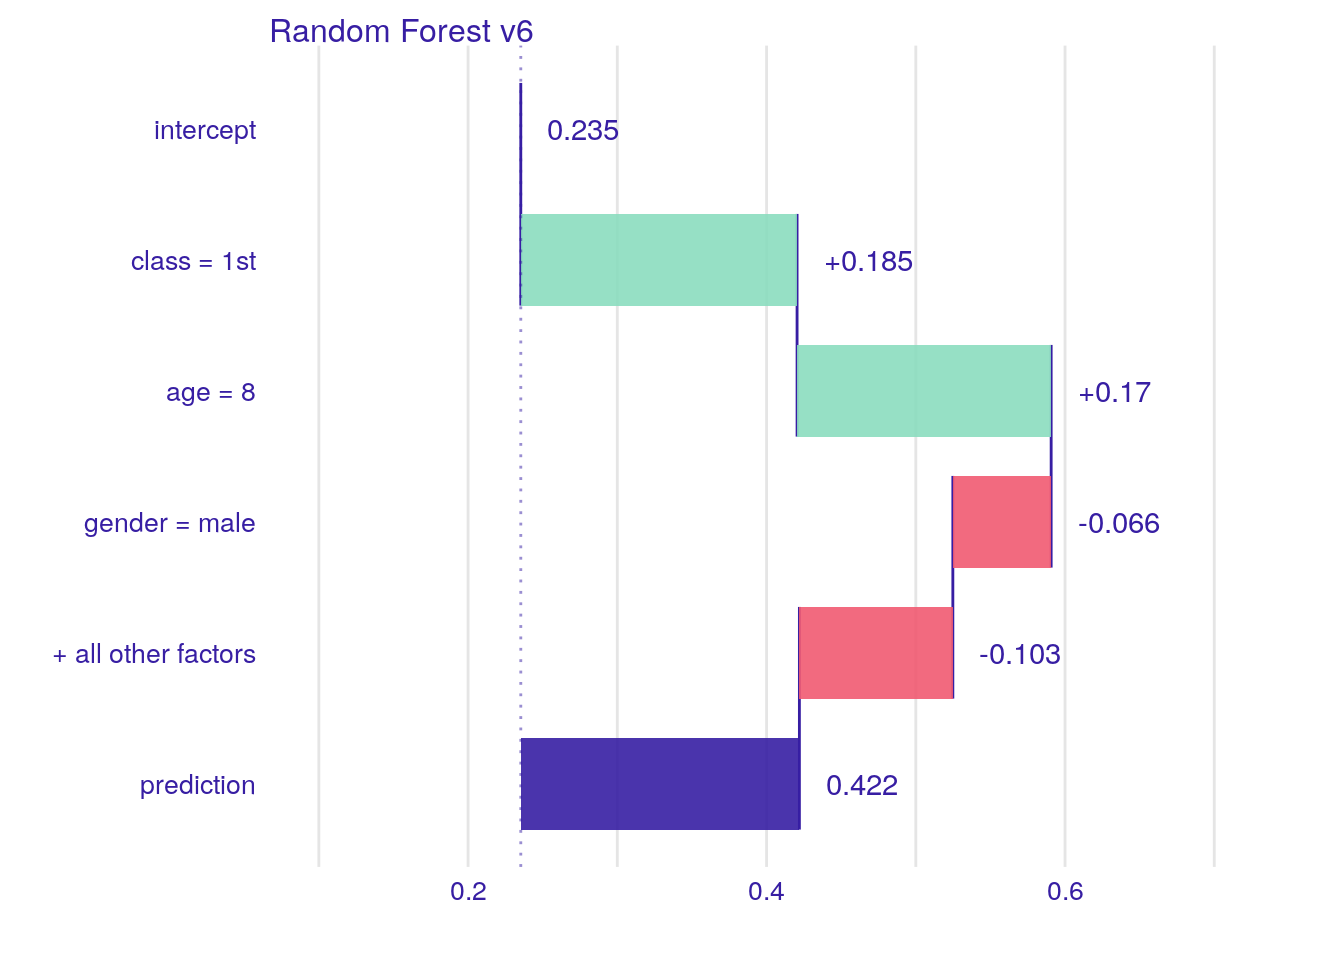
\includegraphics{PM_VEE_files/figure-latex/unnamed-chunk-54-1.pdf}

\begin{Shaded}
\begin{Highlighting}[]
\KeywordTok{plotRROC}\NormalTok{(rf_au, lm_au, svm_au)}
\end{Highlighting}
\end{Shaded}

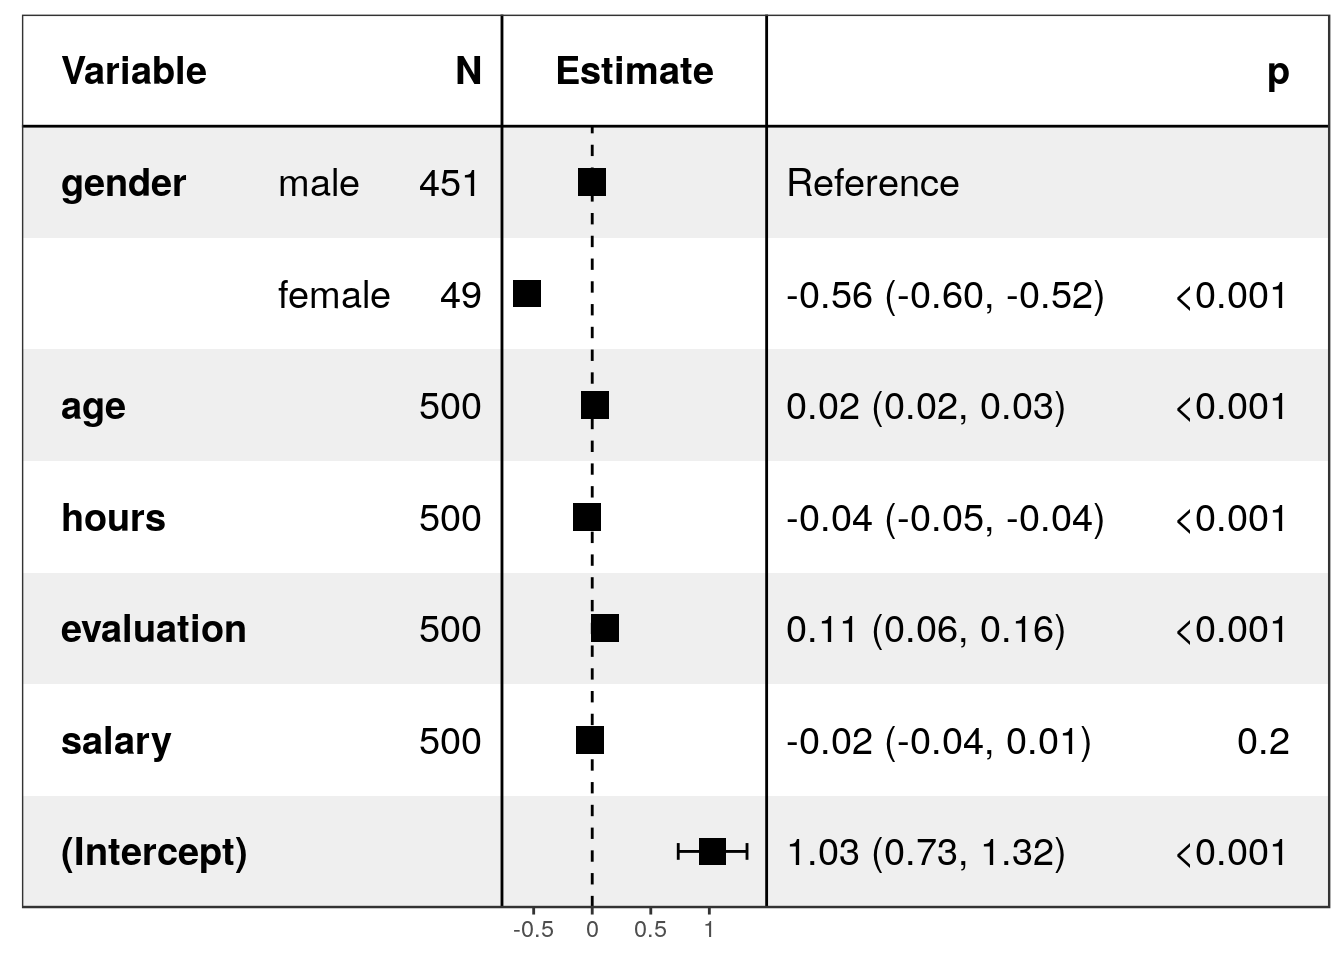
\includegraphics{PM_VEE_files/figure-latex/unnamed-chunk-54-2.pdf}

\hypertarget{modelAuditing}{%
\section{Residual Diagnostic}\label{modelAuditing}}

Goal: verify if model is ok

\citep{R-auditor}

\begin{Shaded}
\begin{Highlighting}[]
\KeywordTok{library}\NormalTok{(}\StringTok{"auditor"}\NormalTok{)}
\KeywordTok{library}\NormalTok{(}\StringTok{"DALEX2"}\NormalTok{)}
\KeywordTok{library}\NormalTok{(}\StringTok{"ranger"}\NormalTok{)}

\NormalTok{rf_model <-}\StringTok{ }\KeywordTok{ranger}\NormalTok{(life_length }\OperatorTok{~}\StringTok{ }\NormalTok{., }\DataTypeTok{data =}\NormalTok{ dragons)}
\NormalTok{predict_function <-}\StringTok{ }\ControlFlowTok{function}\NormalTok{(m,x,...) }\KeywordTok{predict}\NormalTok{(m, x, ...)}\OperatorTok{$}\NormalTok{predictions}
\NormalTok{rf_au <-}\StringTok{ }\KeywordTok{audit}\NormalTok{(rf_model, }\DataTypeTok{data =}\NormalTok{ dragons, }\DataTypeTok{y =}\NormalTok{ dragons}\OperatorTok{$}\NormalTok{life_length,}
           \DataTypeTok{predict.function =}\NormalTok{ predict_function)}
\KeywordTok{check_residuals}\NormalTok{(rf_au)}
\end{Highlighting}
\end{Shaded}

\begin{verbatim}
##   -----------------------------------------------
##    Checks for autocorrelation
##   -----------------------------------------------
##     Model name:  ranger 
##     Autocorrelation in target:     +0.01      
##     Autocorrelation in residuals:  +0.01      
##   -----------------------------------------------
##    Checks for outliers
##   -----------------------------------------------
##     Model name:  ranger 
##     Shift > 1:  20 ( 1 %) 
##     Shift > 2:  14 ( 0.7 %) 
##     Top lowest standardised residuals: 
##      -2.5534 (1888), -2.4594 (920), -2.4588 (1388), -2.4019 (1508), -2.2377 (1829) 
##     Top highest standardised residuals: 
##      15.242 (1914), 11.256 (1745), 9.7175 (1532), 9.6979 (1111), 8.391 (1051) 
##   -----------------------------------------------
##    Checks for trend in residuals
##   -----------------------------------------------
##     Model name:  ranger 
##     Standardised loess fit:  +76.75     ***
\end{verbatim}

\begin{Shaded}
\begin{Highlighting}[]
\KeywordTok{plotResidualBoxplot}\NormalTok{(rf_au)}
\end{Highlighting}
\end{Shaded}

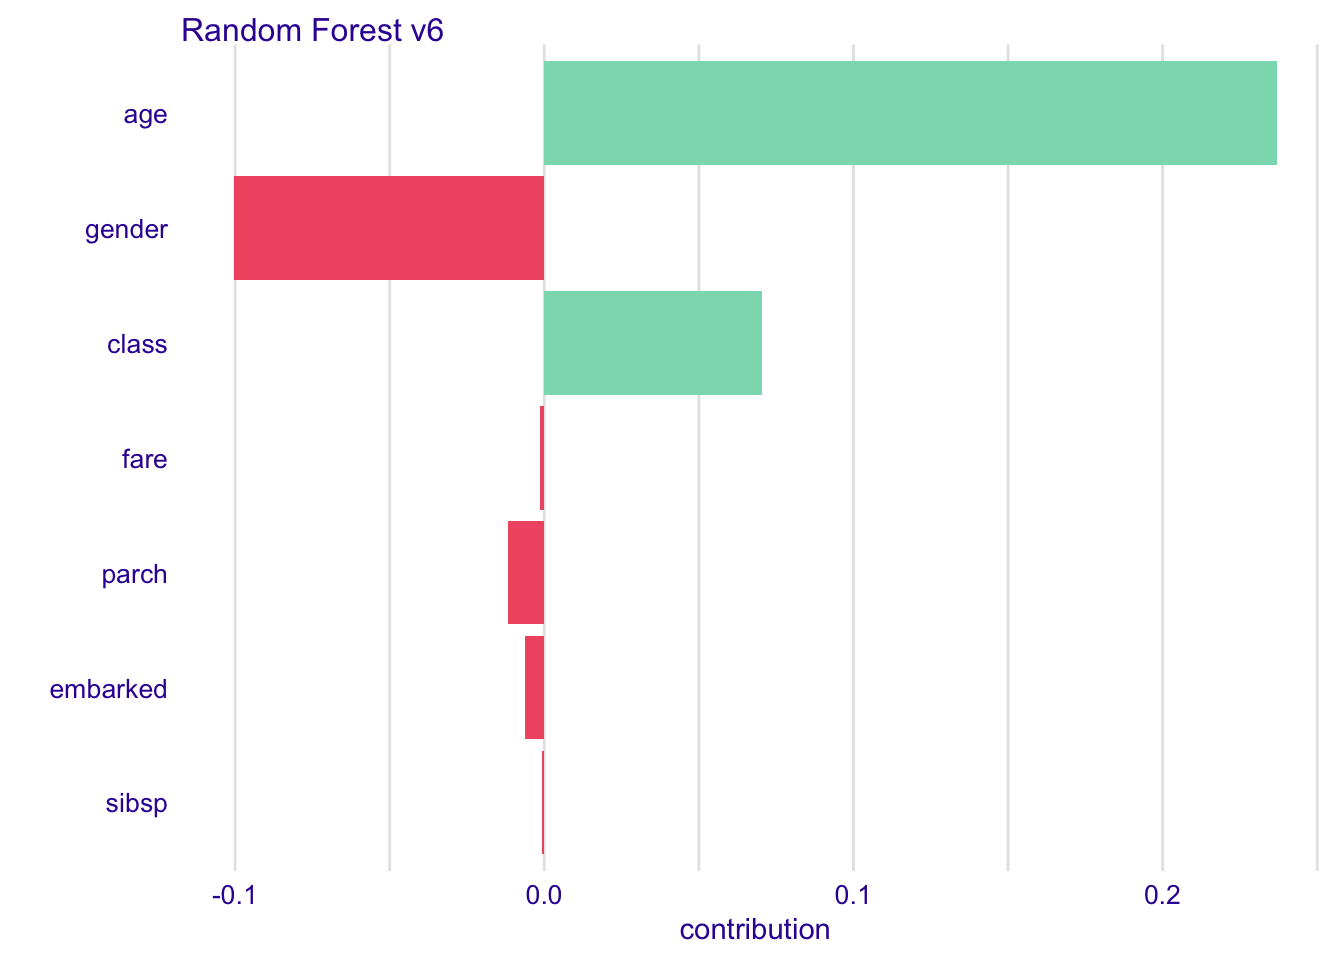
\includegraphics{PM_VEE_files/figure-latex/unnamed-chunk-55-1.pdf}

\begin{Shaded}
\begin{Highlighting}[]
\KeywordTok{plotResidual}\NormalTok{(rf_au, }\DataTypeTok{variable =} \StringTok{"Observed response"}\NormalTok{)}
\end{Highlighting}
\end{Shaded}

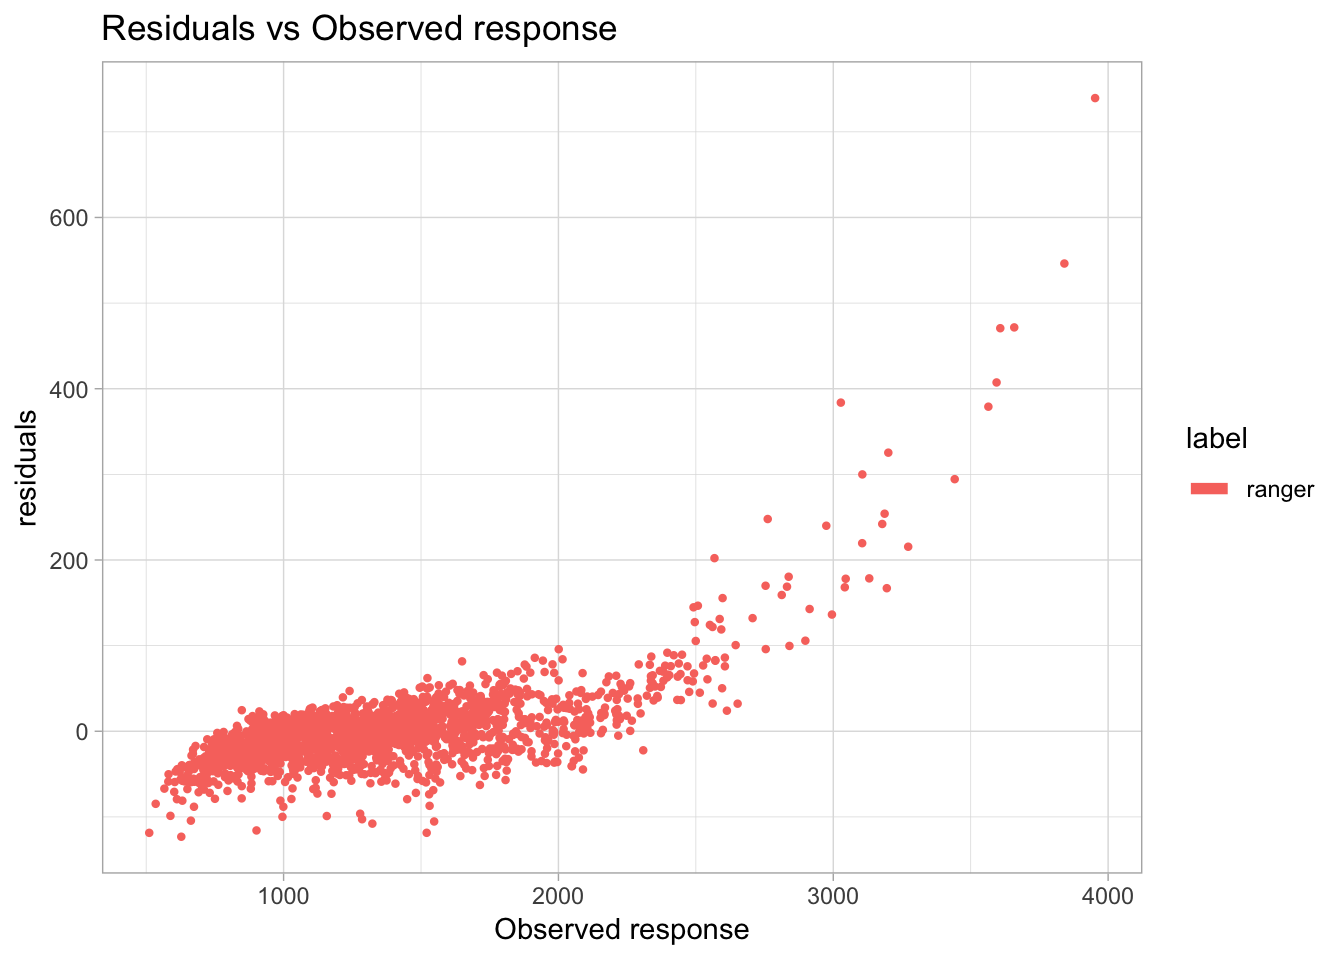
\includegraphics{PM_VEE_files/figure-latex/unnamed-chunk-55-2.pdf}

\begin{Shaded}
\begin{Highlighting}[]
\KeywordTok{plotScaleLocation}\NormalTok{(rf_au)}
\end{Highlighting}
\end{Shaded}

\includegraphics{PM_VEE_files/figure-latex/unnamed-chunk-55-3.pdf}

\begin{Shaded}
\begin{Highlighting}[]
\KeywordTok{plotRROC}\NormalTok{(rf_au)}
\end{Highlighting}
\end{Shaded}

\includegraphics{PM_VEE_files/figure-latex/unnamed-chunk-55-4.pdf}

\begin{Shaded}
\begin{Highlighting}[]
\KeywordTok{plotAutocorrelation}\NormalTok{(rf_au)}
\end{Highlighting}
\end{Shaded}

\includegraphics{PM_VEE_files/figure-latex/unnamed-chunk-55-5.pdf}

\hypertarget{concept-drift}{%
\section{Concept Drift}\label{concept-drift}}

Machine learning models are often fitted and validated on historical
data under silent assumption that data are stationary. The most popular
techniques for validation (k-fold cross-validation, repeated
cross-validation, and so on) test models on data with the same
distribution as training data.

Yet, in many practical applications, deployed models are working in a
changing environment. After some time, due to changes in the
environment, model performance may degenerate, as model may be less
reliable.

Concept drift refers to the change in the data distribution or in the
relationships between variables over time. Think about model for energy
consumption for a school, over time the school may be equipped with
larger number of devices of with more power-efficient devices that may
affect the model performance.

In this chapter we define basic ideas behind concept drift and propose
some solutions.

\hypertarget{introduction-3}{%
\subsection{Introduction}\label{introduction-3}}

In general, concept drift means that some statistical properties of
variables used in the model change over time. This may result in
degenerated performance. Thus the early detection of concept drift is
very important, as it is needed to adapt quickly to these changes.

The term \texttt{concept} usually refers to target variable, but
generally, it can also refer to model input of relations between
variables.

The most general formulation of a concept drift refers to changes in
joint distribution of \(p(X, y)\). It is useful to define also following
measures.

\begin{itemize}
\tightlist
\item
  Conditional Covariate Drift as change in \(p(X | y)\)
\item
  Conditional Class Drift as change in \(p(y | X)\)
\item
  Covariate Drift or Concept Shift as changes in \(p(X)\)
\end{itemize}

Once the drift is detected one may re-fit the model on newer data or
update the model.

\hypertarget{covariate-drift}{%
\subsection{Covariate Drift}\label{covariate-drift}}

Covariate Drift is a change in distribution of input, change in the
distribution of \(p(X)\). The input is a \(p\)-dimensional vector with
variables of possible mixed types and distributions.

Here we propose a simple one-dimensional method, that can be applied to
each variable separately despite of its type. We do not rely on any
formal statistical test, as the power of the test depends on sample size
and for large samples the test will detect even small differences.

We also consider an use-case for two samples. One sample gathers
historical ,,old'' data, this may be data available during the model
development (part of it may be used as training and part as test data).
Second sample is the current ,,new'' data, and we want to know is the
distribution of \(X_{old}\) differs from the distribution of
\(X_{new}\).

There is a lot of distances between probability measures that can be
used here (as for example Wasserstein, Total Variation and so on). We
are using the Non-Intersection Distance due to its easy interpretation.

For categorical variables \(P\) and \(Q\) non-intersection distance is
defined as \[
d(P,Q) = 1 - \sum_{i\in \mathcal X} \min(p_i, q_i)
\] where \(\mathcal X\) is a set of all possible values while \(p_i\)
and \(q_i\) are probabilities for these values in distribution \(P\) and
\(Q\) respectively. An intuition behind this distance is that it's
amount of the distribution \(P\) that is not shared with \(Q\) (it's
symmetric). The smaller the value the closes are these distributions.

For continuous variables we discretize their distribution in the spirit
of \(\chi^2\) test.

\hypertarget{code-snippets-2}{%
\subsection{Code snippets}\label{code-snippets-2}}

Here we are going to use the \texttt{drifter} package that implements
some tools for concept drift detection.

As an illustration we use two datasets from the \texttt{DALEX2} package,
namely \texttt{apartments} (here we do not have drift) and
\texttt{dragons} (here we do have drift).

\begin{Shaded}
\begin{Highlighting}[]
\KeywordTok{library}\NormalTok{(}\StringTok{"DALEX2"}\NormalTok{)}
\KeywordTok{library}\NormalTok{(}\StringTok{"drifter"}\NormalTok{)}

\CommentTok{# here we do not have any drift}
\KeywordTok{head}\NormalTok{(apartments, }\DecValTok{2}\NormalTok{)}
\end{Highlighting}
\end{Shaded}

\begin{verbatim}
##   m2.price construction.year surface floor no.rooms    district
## 1     5897              1953      25     3        1 Srodmiescie
## 2     1818              1992     143     9        5     Bielany
\end{verbatim}

\begin{Shaded}
\begin{Highlighting}[]
\NormalTok{d <-}\StringTok{ }\KeywordTok{calculate_covariate_drift}\NormalTok{(apartments, apartments_test)}
\NormalTok{d}
\end{Highlighting}
\end{Shaded}

\begin{verbatim}
##                   Variable  Shift
##   -------------------------------------
##                   m2.price    4.9  
##          construction.year    6.0  
##                    surface    6.8  
##                      floor    4.9  
##                   no.rooms    2.8  
##                   district    2.8
\end{verbatim}

\begin{Shaded}
\begin{Highlighting}[]
\CommentTok{# here we do have drift}
\KeywordTok{head}\NormalTok{(dragons, }\DecValTok{2}\NormalTok{)}
\end{Highlighting}
\end{Shaded}

\begin{verbatim}
##   year_of_birth   height   weight scars colour year_of_discovery
## 1         -1291 59.40365 15.32391     7    red              1700
## 2          1589 46.21374 11.80819     5    red              1700
##   number_of_lost_teeth life_length
## 1                   25    1368.433
## 2                   28    1377.047
\end{verbatim}

\begin{Shaded}
\begin{Highlighting}[]
\NormalTok{d <-}\StringTok{ }\KeywordTok{calculate_covariate_drift}\NormalTok{(dragons, dragons_test)}
\NormalTok{d}
\end{Highlighting}
\end{Shaded}

\begin{verbatim}
##                   Variable  Shift
##   -------------------------------------
##              year_of_birth    8.9  
##                     height   15.3  .
##                     weight   14.7  .
##                      scars    4.6  
##                     colour   17.9  .
##          year_of_discovery   97.5  ***
##       number_of_lost_teeth    6.3  
##                life_length    8.6
\end{verbatim}

\hypertarget{residual-drift}{%
\subsection{Residual Drift}\label{residual-drift}}

Perhaps the most obvious negative effect of the concept drift is that
the model performance degrades over time.

But this is also something that is straightforward to verify. One can
calculate distribution of residuals on new data and compare this
distribution with residuals obtained on old data.

Again, we have two samples, residuals calculated on the old dataset

\[
r_{old} = y_{old} - \hat y_{old} = y_{old} - f_{old}(X_{old})
\] versus residuals calculated on the new dataset \[
r_{new} = y_{new} - \hat y_{new} = y_{new} - f_{old}(X_{new})
\]

We can use any distance between distributions to compare \(r_{new}\) and
\(r_{old}\), for example the non-intersection distance.

\hypertarget{code-snippets-3}{%
\subsection{Code snippets}\label{code-snippets-3}}

Here we are going to use the \texttt{drifter} package.

\begin{Shaded}
\begin{Highlighting}[]
\KeywordTok{library}\NormalTok{(}\StringTok{"DALEX2"}\NormalTok{)}
\KeywordTok{library}\NormalTok{(}\StringTok{"drifter"}\NormalTok{)}
\KeywordTok{library}\NormalTok{(}\StringTok{"ranger"}\NormalTok{)}

\NormalTok{data_old <-}\StringTok{ }\NormalTok{apartments_test[}\DecValTok{1}\OperatorTok{:}\DecValTok{4000}\NormalTok{,]}
\NormalTok{data_new <-}\StringTok{ }\NormalTok{apartments_test[}\DecValTok{4001}\OperatorTok{:}\DecValTok{8000}\NormalTok{,]}

\NormalTok{predict_function <-}\StringTok{ }\ControlFlowTok{function}\NormalTok{(m,x,...) }\KeywordTok{predict}\NormalTok{(m, x, ...)}\OperatorTok{$}\NormalTok{predictions}
\NormalTok{model_old <-}\StringTok{ }\KeywordTok{ranger}\NormalTok{(m2.price }\OperatorTok{~}\StringTok{ }\NormalTok{., }\DataTypeTok{data =}\NormalTok{ apartments)}
\KeywordTok{calculate_residuals_drift}\NormalTok{(model_old,}
\NormalTok{                      data_old, data_new,}
\NormalTok{                      data_old}\OperatorTok{$}\NormalTok{m2.price, }
\NormalTok{                      data_new}\OperatorTok{$}\NormalTok{m2.price,}
                      \DataTypeTok{predict_function =}\NormalTok{ predict_function)}
\end{Highlighting}
\end{Shaded}

\begin{verbatim}
##                   Variable  Shift
##   -------------------------------------
##                  Residuals    3.4
\end{verbatim}

\hypertarget{model-drift}{%
\subsection{Model Drift}\label{model-drift}}

Model Drift is a change in the relation between target variable and
input variables, change in \(p(y|X)\). The input is a \(p\)-dimensional
vector with variables of possible mixed types and distributions.

Here we propose a simple one-dimensional method based on Partial
Dependency Plots introduced in the Chapter \ref{partialDependence}. PDP
profiles summaries marginal relation between \(\hat y\) and variable
\(x_i\). The idea behind concept drift is to compare two models, the old
model \(f_{old}\) and model refitted on the new data \(f_{new}\) and
compare these models through PDP profiles.

For each variable we can obtain scores for drift calculated as \(L_2\)
distance between PDP profiles for both models.

\[
drift_{i} = \frac 1 {|Z_i|}\int_{z\in Z_i} (PDP_i(f_{old}) - PDP_i(f_{new}))^2 dz
\] where \(Z_i\) is the set of values for variable \(x_i\) (for
simplicity we assume that it's an interval) while \(PDP_i(f_{new})\) is
the PDP profile for variable \(i\) calculated for the model \(f_{new}\).

\hypertarget{code-snippets-4}{%
\subsection{Code snippets}\label{code-snippets-4}}

Here we are going to use the \texttt{drifter} package. Instead of using
\texttt{old} and \texttt{new} data here we compare model trained on data
with males versus new dataset that contain data for females.

But, because of the interaction of gender and age, models created on
these two datasets are different.

\begin{Shaded}
\begin{Highlighting}[]
\KeywordTok{library}\NormalTok{(}\StringTok{"DALEX2"}\NormalTok{)}
\KeywordTok{library}\NormalTok{(}\StringTok{"drifter"}\NormalTok{)}
\KeywordTok{library}\NormalTok{(}\StringTok{"ranger"}\NormalTok{)}

\NormalTok{predict_function <-}\StringTok{ }\ControlFlowTok{function}\NormalTok{(m,x,...) }\KeywordTok{predict}\NormalTok{(m, x, ..., }\DataTypeTok{probability=}\OtherTok{TRUE}\NormalTok{)}\OperatorTok{$}\NormalTok{predictions[,}\DecValTok{1}\NormalTok{]}
\NormalTok{data_old =}\StringTok{ }\NormalTok{HR[HR}\OperatorTok{$}\NormalTok{gender }\OperatorTok{==}\StringTok{ "male"}\NormalTok{, }\DecValTok{-1}\NormalTok{]}
\NormalTok{data_new =}\StringTok{ }\NormalTok{HR[HR}\OperatorTok{$}\NormalTok{gender }\OperatorTok{==}\StringTok{ "female"}\NormalTok{, }\DecValTok{-1}\NormalTok{]}
\NormalTok{model_old <-}\StringTok{ }\KeywordTok{ranger}\NormalTok{(status }\OperatorTok{~}\StringTok{ }\NormalTok{., }\DataTypeTok{data =}\NormalTok{ data_old, }\DataTypeTok{probability =} \OtherTok{TRUE}\NormalTok{)}
\NormalTok{model_new <-}\StringTok{ }\KeywordTok{ranger}\NormalTok{(status }\OperatorTok{~}\StringTok{ }\NormalTok{., }\DataTypeTok{data =}\NormalTok{ data_new, }\DataTypeTok{probability =} \OtherTok{TRUE}\NormalTok{)}
\KeywordTok{calculate_model_drift}\NormalTok{(model_old, model_new,}
\NormalTok{                 HR_test,}
\NormalTok{                 HR_test}\OperatorTok{$}\NormalTok{status }\OperatorTok{==}\StringTok{ "fired"}\NormalTok{,}
                 \DataTypeTok{max_obs =} \DecValTok{1000}\NormalTok{,}
                 \DataTypeTok{predict_function =}\NormalTok{ predict_function)}
\end{Highlighting}
\end{Shaded}

\begin{verbatim}
##                   Variable    Shift  Scaled
##   -----------------------------------------------
##                     gender     0.00     0.9  
##                        age     0.26    54.7  ***
##                      hours     0.04     8.3  
##                 evaluation     0.01     2.6  
##                     salary     0.02     3.4  
##                     status     0.00     0.9
\end{verbatim}

\begin{Shaded}
\begin{Highlighting}[]
\KeywordTok{library}\NormalTok{(}\StringTok{"ceterisParibus2"}\NormalTok{)}
\NormalTok{prof_old <-}\StringTok{ }\KeywordTok{individual_variable_profile}\NormalTok{(model_old,}
                 \DataTypeTok{data =}\NormalTok{ data_new,}
                 \DataTypeTok{new_observation =}\NormalTok{ data_new[}\DecValTok{1}\OperatorTok{:}\DecValTok{1000}\NormalTok{,],}
                 \DataTypeTok{label =} \StringTok{"model_old"}\NormalTok{,}
                 \DataTypeTok{predict_function =}\NormalTok{ predict_function)}
\NormalTok{prof_new <-}\StringTok{ }\KeywordTok{individual_variable_profile}\NormalTok{(model_new,}
                 \DataTypeTok{data =}\NormalTok{ data_new,}
                 \DataTypeTok{new_observation =}\NormalTok{ data_new[}\DecValTok{1}\OperatorTok{:}\DecValTok{1000}\NormalTok{,],}
                 \DataTypeTok{label =} \StringTok{"model_new"}\NormalTok{,}
                 \DataTypeTok{predict_function =}\NormalTok{ predict_function)}
\KeywordTok{plot}\NormalTok{(prof_old, prof_new,}
     \DataTypeTok{selected_variables =} \StringTok{"age"}\NormalTok{, }\DataTypeTok{aggregate_profiles =}\NormalTok{ mean,}
     \DataTypeTok{show_observations =} \OtherTok{FALSE}\NormalTok{, }\DataTypeTok{color =} \StringTok{"_label_"}\NormalTok{, }\DataTypeTok{alpha =} \DecValTok{1}\NormalTok{)}
\end{Highlighting}
\end{Shaded}

\includegraphics{PM_VEE_files/figure-latex/unnamed-chunk-58-1.pdf}

\hypertarget{appendixes}{%
\section*{Appendixes}\label{appendixes}}
\addcontentsline{toc}{section}{Appendixes}

\hypertarget{DataSets}{%
\section{Data Sets}\label{DataSets}}

\hypertarget{TitanicDataset}{%
\subsection{Predict survival on the Titanic}\label{TitanicDataset}}

Sinking of the RMS Titanic is one of the deadliest maritime disasters in
history (during peacetime). Over 1500 people died as a consequence of
collision with an iceberg. Thanks to projects like \emph{Encyclopedia
titanica} \texttt{https://www.encyclopedia-titanica.org/} we have a very
rich and precise data about passagers. This dataset is avaliable in the
\texttt{titanic} dataset.

\begin{Shaded}
\begin{Highlighting}[]
\KeywordTok{library}\NormalTok{(}\StringTok{"titanic"}\NormalTok{)}
\KeywordTok{head}\NormalTok{(titanic_train)}
\end{Highlighting}
\end{Shaded}

\begin{verbatim}
##   PassengerId Survived Pclass
## 1           1        0      3
## 2           2        1      1
## 3           3        1      3
## 4           4        1      1
## 5           5        0      3
## 6           6        0      3
##                                                  Name    Sex Age SibSp
## 1                             Braund, Mr. Owen Harris   male  22     1
## 2 Cumings, Mrs. John Bradley (Florence Briggs Thayer) female  38     1
## 3                              Heikkinen, Miss. Laina female  26     0
## 4        Futrelle, Mrs. Jacques Heath (Lily May Peel) female  35     1
## 5                            Allen, Mr. William Henry   male  35     0
## 6                                    Moran, Mr. James   male  NA     0
##   Parch           Ticket    Fare Cabin Embarked
## 1     0        A/5 21171  7.2500              S
## 2     0         PC 17599 71.2833   C85        C
## 3     0 STON/O2. 3101282  7.9250              S
## 4     0           113803 53.1000  C123        S
## 5     0           373450  8.0500              S
## 6     0           330877  8.4583              Q
\end{verbatim}

Feature of interest is the binary variable \texttt{Survived}. Let's
build some predictive models for this variable.

First we need to do some data preprocessing.

\begin{Shaded}
\begin{Highlighting}[]
\NormalTok{titanic_small <-}\StringTok{ }\NormalTok{titanic_train[,}\KeywordTok{c}\NormalTok{(}\StringTok{"Survived"}\NormalTok{, }\StringTok{"Pclass"}\NormalTok{, }\StringTok{"Sex"}\NormalTok{, }\StringTok{"Age"}\NormalTok{, }\StringTok{"SibSp"}\NormalTok{, }\StringTok{"Parch"}\NormalTok{, }\StringTok{"Fare"}\NormalTok{, }\StringTok{"Embarked"}\NormalTok{)]}
\NormalTok{titanic_small}\OperatorTok{$}\NormalTok{Survived <-}\StringTok{ }\KeywordTok{factor}\NormalTok{(titanic_small}\OperatorTok{$}\NormalTok{Survived)}
\NormalTok{titanic_small}\OperatorTok{$}\NormalTok{Sex <-}\StringTok{ }\KeywordTok{factor}\NormalTok{(titanic_small}\OperatorTok{$}\NormalTok{Sex)}
\NormalTok{titanic_small}\OperatorTok{$}\NormalTok{Embarked <-}\StringTok{ }\KeywordTok{factor}\NormalTok{(titanic_small}\OperatorTok{$}\NormalTok{Embarked)}
\NormalTok{titanic_small <-}\StringTok{ }\KeywordTok{na.omit}\NormalTok{(titanic_small)}

\NormalTok{titanic_train[}\DecValTok{760}\NormalTok{,]}
\end{Highlighting}
\end{Shaded}

\begin{verbatim}
##     PassengerId Survived Pclass
## 760         760        1      1
##                                                         Name    Sex Age
## 760 Rothes, the Countess. of (Lucy Noel Martha Dyer-Edwards) female  33
##     SibSp Parch Ticket Fare Cabin Embarked
## 760     0     0 110152 86.5   B77        S
\end{verbatim}

\begin{Shaded}
\begin{Highlighting}[]
\NormalTok{titanic_small[}\DecValTok{760}\NormalTok{,]}
\end{Highlighting}
\end{Shaded}

\begin{verbatim}
##    Survived Pclass  Sex Age SibSp Parch Fare Embarked
## NA     <NA>     NA <NA>  NA    NA    NA   NA     <NA>
\end{verbatim}

\hypertarget{random-forest}{%
\subsubsection{Random Forest}\label{random-forest}}

Now we can create models. Let's start with Random Forest

\begin{Shaded}
\begin{Highlighting}[]
\KeywordTok{library}\NormalTok{(}\StringTok{"randomForest"}\NormalTok{)}
\NormalTok{rf_model <-}\StringTok{ }\KeywordTok{randomForest}\NormalTok{(Survived }\OperatorTok{~}\StringTok{ }\NormalTok{Pclass }\OperatorTok{+}\StringTok{ }\NormalTok{Sex }\OperatorTok{+}\StringTok{ }\NormalTok{Age }\OperatorTok{+}\StringTok{ }\NormalTok{SibSp }\OperatorTok{+}\StringTok{ }
\StringTok{                           }\NormalTok{Parch }\OperatorTok{+}\StringTok{ }\NormalTok{Fare }\OperatorTok{+}\StringTok{ }\NormalTok{Embarked, }
                           \DataTypeTok{data =}\NormalTok{ titanic_small)}
\NormalTok{rf_model}
\end{Highlighting}
\end{Shaded}

\begin{verbatim}
## 
## Call:
##  randomForest(formula = Survived ~ Pclass + Sex + Age + SibSp +      Parch + Fare + Embarked, data = titanic_small) 
##                Type of random forest: classification
##                      Number of trees: 500
## No. of variables tried at each split: 2
## 
##         OOB estimate of  error rate: 19.19%
## Confusion matrix:
##     0   1 class.error
## 0 379  45   0.1061321
## 1  92 198   0.3172414
\end{verbatim}

\hypertarget{logistic-regression}{%
\subsubsection{Logistic regression}\label{logistic-regression}}

Logistic model is a generalized linear moedl with binomial family and
logit link function.

\begin{Shaded}
\begin{Highlighting}[]
\NormalTok{glm_model <-}\StringTok{ }\KeywordTok{glm}\NormalTok{(Survived }\OperatorTok{~}\StringTok{ }\NormalTok{Pclass }\OperatorTok{+}\StringTok{ }\NormalTok{Sex }\OperatorTok{+}\StringTok{ }\NormalTok{Age }\OperatorTok{+}\StringTok{ }\NormalTok{SibSp }\OperatorTok{+}\StringTok{ }\NormalTok{Parch }\OperatorTok{+}\StringTok{ }\NormalTok{Fare }\OperatorTok{+}\StringTok{ }\NormalTok{Embarked,}
                         \DataTypeTok{data =}\NormalTok{ titanic_small, }\DataTypeTok{family =} \StringTok{"binomial"}\NormalTok{)}
\KeywordTok{summary}\NormalTok{(glm_model)}
\end{Highlighting}
\end{Shaded}

\begin{verbatim}
## 
## Call:
## glm(formula = Survived ~ Pclass + Sex + Age + SibSp + Parch + 
##     Fare + Embarked, family = "binomial", data = titanic_small)
## 
## Deviance Residuals: 
##     Min       1Q   Median       3Q      Max  
## -2.7233  -0.6439  -0.3772   0.6288   2.4457  
## 
## Coefficients:
##               Estimate Std. Error z value Pr(>|z|)    
## (Intercept)  17.894850 607.855474   0.029  0.97651    
## Pclass       -1.199251   0.164619  -7.285 3.22e-13 ***
## Sexmale      -2.638476   0.222256 -11.871  < 2e-16 ***
## Age          -0.043350   0.008232  -5.266 1.39e-07 ***
## SibSp        -0.363208   0.129017  -2.815  0.00487 ** 
## Parch        -0.060270   0.123900  -0.486  0.62666    
## Fare          0.001432   0.002531   0.566  0.57165    
## EmbarkedC   -12.257443 607.855250  -0.020  0.98391    
## EmbarkedQ   -13.080988 607.855452  -0.022  0.98283    
## EmbarkedS   -12.658656 607.855228  -0.021  0.98339    
## ---
## Signif. codes:  0 '***' 0.001 '**' 0.01 '*' 0.05 '.' 0.1 ' ' 1
## 
## (Dispersion parameter for binomial family taken to be 1)
## 
##     Null deviance: 964.52  on 713  degrees of freedom
## Residual deviance: 632.34  on 704  degrees of freedom
## AIC: 652.34
## 
## Number of Fisher Scoring iterations: 13
\end{verbatim}

\hypertarget{splines-with-rms}{%
\subsubsection{Splines with RMS}\label{splines-with-rms}}

\begin{Shaded}
\begin{Highlighting}[]
\KeywordTok{library}\NormalTok{(}\StringTok{"rms"}\NormalTok{)}
\NormalTok{rms_model <-}\StringTok{ }\KeywordTok{lrm}\NormalTok{(Survived }\OperatorTok{==}\StringTok{ "1"} \OperatorTok{~}\StringTok{ }\NormalTok{Pclass }\OperatorTok{+}\StringTok{ }\NormalTok{Sex }\OperatorTok{+}\StringTok{ }\KeywordTok{rcs}\NormalTok{(Age) }\OperatorTok{+}\StringTok{ }\NormalTok{SibSp }\OperatorTok{+}
\StringTok{                   }\NormalTok{Parch }\OperatorTok{+}\StringTok{ }\NormalTok{Fare }\OperatorTok{+}\StringTok{ }\NormalTok{Embarked, titanic_small)}
\NormalTok{rms_model}
\end{Highlighting}
\end{Shaded}

\begin{verbatim}
## Logistic Regression Model
##  
##  lrm(formula = Survived == "1" ~ Pclass + Sex + rcs(Age) + SibSp + 
##      Parch + Fare + Embarked, data = titanic_small)
##  
##                      Model Likelihood     Discrimination    Rank Discrim.    
##                         Ratio Test           Indexes           Indexes       
##  Obs         714    LR chi2     353.20    R2       0.527    C       0.874    
##   FALSE      424    d.f.            12    g        2.192    Dxy     0.748    
##   TRUE       290    Pr(> chi2) <0.0001    gr       8.957    gamma   0.749    
##  max |deriv| 0.1                          gp       0.363    tau-a   0.361    
##                                           Brier    0.134                     
##  
##             Coef    S.E.    Wald Z Pr(>|Z|)
##  Intercept  12.1530 26.3889   0.46 0.6451  
##  Pclass     -1.0822  0.1693  -6.39 <0.0001 
##  Sex=male   -2.7848  0.2317 -12.02 <0.0001 
##  Age        -0.2382  0.0472  -5.04 <0.0001 
##  Age'        0.7961  0.2138   3.72 0.0002  
##  Age''      -4.3833  1.5123  -2.90 0.0038  
##  Age'''      5.1859  2.2693   2.29 0.0223  
##  SibSp      -0.5292  0.1449  -3.65 0.0003  
##  Parch      -0.1990  0.1344  -1.48 0.1387  
##  Fare        0.0032  0.0029   1.11 0.2670  
##  Embarked=C -4.6054 26.3806  -0.17 0.8614  
##  Embarked=Q -5.3341 26.3853  -0.20 0.8398  
##  Embarked=S -4.9968 26.3802  -0.19 0.8498  
## 
\end{verbatim}

\hypertarget{gradient-boosting}{%
\subsubsection{Gradient boosting}\label{gradient-boosting}}

\begin{Shaded}
\begin{Highlighting}[]
\KeywordTok{library}\NormalTok{(}\StringTok{"gbm"}\NormalTok{)}
\NormalTok{titanic_gbm <-}\StringTok{ }\KeywordTok{gbm}\NormalTok{(Survived }\OperatorTok{==}\StringTok{ "1"} \OperatorTok{~}\StringTok{ }\NormalTok{Pclass }\OperatorTok{+}\StringTok{ }\NormalTok{Sex }\OperatorTok{+}\StringTok{ }\NormalTok{Age }\OperatorTok{+}\StringTok{ }\NormalTok{SibSp }\OperatorTok{+}
\StringTok{                     }\NormalTok{Parch }\OperatorTok{+}\StringTok{ }\NormalTok{Fare }\OperatorTok{+}\StringTok{ }\NormalTok{Embarked, }\DataTypeTok{data =}\NormalTok{ titanic_small, }\DataTypeTok{n.trees =} \DecValTok{15000}\NormalTok{)}
\end{Highlighting}
\end{Shaded}

\begin{verbatim}
## Distribution not specified, assuming bernoulli ...
\end{verbatim}

\begin{Shaded}
\begin{Highlighting}[]
\NormalTok{titanic_gbm}
\end{Highlighting}
\end{Shaded}

\begin{verbatim}
## gbm(formula = Survived == "1" ~ Pclass + Sex + Age + SibSp + 
##     Parch + Fare + Embarked, data = titanic_small, n.trees = 15000)
## A gradient boosted model with bernoulli loss function.
## 15000 iterations were performed.
## There were 7 predictors of which 7 had non-zero influence.
\end{verbatim}

\hypertarget{HRdataset}{%
\subsection{Hire or Fire? HR in Call Center}\label{HRdataset}}

In this chapter we present an artificial dataset from Human Resources
department in a Call Center.

The dataset is available in the \texttt{DALEX} package \citep{R-DALEX}.
Each row corresponds to a single employee in a call center. Features
like gender, age, average number of working hours per week, grade from
the last evaluation and level of salary are used as predictive features.

The goal here is to first build a model, that will guess when to fire
and when to promote an employer, so it's a classification problem with
three classes.

Why we need such model? We want to have objective decisions. That will
not be subject to personal preferences of a manager. But is it possible
to have an objective model? Would it be fair or it will just replicate
some unfairness?

We will use this example to show how to use prediction level explainers
to better understand how the model works for selected cases.

\begin{Shaded}
\begin{Highlighting}[]
\KeywordTok{library}\NormalTok{(}\StringTok{"DALEX"}\NormalTok{)}
\KeywordTok{head}\NormalTok{(HR)}
\end{Highlighting}
\end{Shaded}

\begin{verbatim}
##   gender      age    hours evaluation salary   status
## 1   male 32.58267 41.88626          3      1    fired
## 2 female 41.21104 36.34339          2      5    fired
## 3   male 37.70516 36.81718          3      0    fired
## 4 female 30.06051 38.96032          3      2    fired
## 5   male 21.10283 62.15464          5      3 promoted
## 6   male 40.11812 69.53973          2      0    fired
\end{verbatim}

In this book we are focused on model exploration rather than model
building, thus for sake ok simplicity we will use two default models
created with random forest \citep{R-randomForest} and generalized linear
model \citep{R-nnet}.

\begin{Shaded}
\begin{Highlighting}[]
\KeywordTok{set.seed}\NormalTok{(}\DecValTok{59}\NormalTok{)}
\KeywordTok{library}\NormalTok{(}\StringTok{"randomForest"}\NormalTok{)}
\NormalTok{model_rf <-}\StringTok{ }\KeywordTok{randomForest}\NormalTok{(status }\OperatorTok{~}\StringTok{ }\NormalTok{gender }\OperatorTok{+}\StringTok{ }\NormalTok{age }\OperatorTok{+}\StringTok{ }\NormalTok{hours }\OperatorTok{+}\StringTok{ }\NormalTok{evaluation }\OperatorTok{+}\StringTok{ }\NormalTok{salary, }\DataTypeTok{data =}\NormalTok{ HR)}

\KeywordTok{library}\NormalTok{(}\StringTok{"nnet"}\NormalTok{)}
\NormalTok{model_glm <-}\StringTok{ }\KeywordTok{multinom}\NormalTok{(status }\OperatorTok{~}\StringTok{ }\NormalTok{gender }\OperatorTok{+}\StringTok{ }\NormalTok{age }\OperatorTok{+}\StringTok{ }\NormalTok{hours }\OperatorTok{+}\StringTok{ }\NormalTok{evaluation }\OperatorTok{+}\StringTok{ }\NormalTok{salary, }\DataTypeTok{data =}\NormalTok{ HR)}
\end{Highlighting}
\end{Shaded}

\begin{verbatim}
## # weights:  21 (12 variable)
## initial  value 8620.810629 
## iter  10 value 7002.127738
## iter  20 value 6239.478146
## iter  20 value 6239.478126
## iter  20 value 6239.478124
## final  value 6239.478124 
## converged
\end{verbatim}

\hypertarget{apartmentsDataset}{%
\subsection{How much does it cost? Price prediction for a square
meter}\label{apartmentsDataset}}

In this chapter we present an artificial dataset related to prediction
of prices for appartments in Warsaw. This dataset wil be used to discuss
pros and cons for different techniques of model level explainers.

The dataset is available in the \texttt{DALEX} package \citep{R-DALEX}.
Each row corresponds to a single apartment. Features like surface,
number of rooms, district or floor are used as predictive features.

The problem here is to predict price of a square meter for an
appartment, so it's a regression problem with continouse outcome.

\begin{Shaded}
\begin{Highlighting}[]
\KeywordTok{library}\NormalTok{(}\StringTok{"DALEX"}\NormalTok{)}
\KeywordTok{head}\NormalTok{(apartments)}
\end{Highlighting}
\end{Shaded}

\begin{verbatim}
##   m2.price construction.year surface floor no.rooms    district
## 1     5897              1953      25     3        1 Srodmiescie
## 2     1818              1992     143     9        5     Bielany
## 3     3643              1937      56     1        2       Praga
## 4     3517              1995      93     7        3      Ochota
## 5     3013              1992     144     6        5     Mokotow
## 6     5795              1926      61     6        2 Srodmiescie
\end{verbatim}

The goal here is to predict average price for square meter for an
apartment. Let's build a random forest model with \texttt{randomForest}
package \citep{R-randomForest}.

\begin{Shaded}
\begin{Highlighting}[]
\KeywordTok{library}\NormalTok{(}\StringTok{"randomForest"}\NormalTok{)}
\NormalTok{model_rf <-}\StringTok{ }\KeywordTok{randomForest}\NormalTok{(m2.price }\OperatorTok{~}\StringTok{ }\NormalTok{construction.year }\OperatorTok{+}\StringTok{ }\NormalTok{surface }\OperatorTok{+}\StringTok{ }\NormalTok{floor }\OperatorTok{+}\StringTok{ }\NormalTok{no.rooms }\OperatorTok{+}\StringTok{ }\NormalTok{district, }\DataTypeTok{data =}\NormalTok{ apartments)}
\NormalTok{model_rf}
\end{Highlighting}
\end{Shaded}

\begin{verbatim}
## 
## Call:
##  randomForest(formula = m2.price ~ construction.year + surface +      floor + no.rooms + district, data = apartments) 
##                Type of random forest: regression
##                      Number of trees: 500
## No. of variables tried at each split: 1
## 
##           Mean of squared residuals: 82079.37
##                     % Var explained: 90.01
\end{verbatim}

And a linear model.

\begin{Shaded}
\begin{Highlighting}[]
\NormalTok{model_lm <-}\StringTok{ }\KeywordTok{lm}\NormalTok{(m2.price }\OperatorTok{~}\StringTok{ }\NormalTok{construction.year }\OperatorTok{+}\StringTok{ }\NormalTok{surface }\OperatorTok{+}\StringTok{ }\NormalTok{floor }\OperatorTok{+}\StringTok{ }\NormalTok{no.rooms }\OperatorTok{+}\StringTok{ }\NormalTok{district, }\DataTypeTok{data =}\NormalTok{ apartments)}
\NormalTok{model_lm}
\end{Highlighting}
\end{Shaded}

\begin{verbatim}
## 
## Call:
## lm(formula = m2.price ~ construction.year + surface + floor + 
##     no.rooms + district, data = apartments)
## 
## Coefficients:
##         (Intercept)    construction.year              surface  
##            5020.139               -0.229              -10.238  
##               floor             no.rooms      districtBielany  
##             -99.482              -37.730               17.214  
##     districtMokotow       districtOchota        districtPraga  
##             918.380              926.254              -37.105  
## districtSrodmiescie        districtUrsus      districtUrsynow  
##            2080.611               29.942              -18.865  
##        districtWola     districtZoliborz  
##             -16.891              889.973
\end{verbatim}

\hypertarget{Packages}{%
\section{Packages}\label{Packages}}

\hypertarget{arguments}{%
\subsection{Arguments}\label{arguments}}

Here we present list of arguments in explainers from \texttt{DrWhy}. All
explainers use unified set of arguments. All of them are generic with
two specific implementations \texttt{*.explainer} and
\texttt{*.default}. The first one is working for objects created with
\texttt{DALEX2::explain()} function.

Common core of arguments

\begin{itemize}
\tightlist
\item
  \texttt{x} a model to be explained, or an explainer created with
  function \texttt{DALEX2::explain()}.
\item
  \texttt{data} validation dataset. Used to determine univariate
  distributions, calculation of quantiles, correlations and so on. It
  will be extracted from \texttt{x} if it's an explainer.
\item
  \texttt{predict\_function} predict function that operates on the model
  \texttt{x}. Since the model is a black box, the
  \texttt{predict\_function} is the only interface to access values from
  the model. It should be a function that takes at least a model
  \texttt{x} and \texttt{data} and returns vector of predictions. If
  model response has more than a single number (like multiclass models)
  then this function should return a marix/data.frame of the size
  \texttt{m} x \texttt{d}, where \texttt{m} is the number of
  observations while \texttt{d} is the dimensionality of model response.
  It will be extracted from \texttt{x} if it's an explainer.
\item
  \texttt{new\_observation} an observation/observations to be explained.
  Required for local/instance level explainers. Columns in should
  correspond to columns in the \texttt{data} argument.
\item
  \texttt{...} other parameters.
\item
  \texttt{label} name of the model. By default it's extracted from the
  \texttt{class} attribute of the model
\end{itemize}

Function specific arguments

\begin{itemize}
\tightlist
\item
  \texttt{keep\_distributions} if \texttt{TRUE}, then distributions of
  partial predictions is stored and can be plotted with the generic
  \texttt{plot()}.
\end{itemize}

\bibliography{book.bib,packages.bib}


\end{document}
